\documentclass[twocolumn]{aastex631}
\bibliographystyle{aasjournal}
\usepackage{amsmath}
\usepackage{amssymb}
\usepackage{amsfonts}
\usepackage{mathtools}
\usepackage{url}
\usepackage{booktabs} 
\usepackage{algorithm2e}
\usepackage{array}
\newcommand{\done}{{\tt d1}}
\newcommand{\dnine}{{\tt d9}}
\newcommand{\deleven}{{\tt d11}}

\usepackage{color}
\newcommand{\bsh}[1]{\textcolor{red}{(BSH: #1)}}
\newcommand{\giuse}[1]{\textcolor{orange}{(GP: #1)}}
\newcommand{\sg}[1]{\textcolor{teal}{(SG: #1)}}
\newcommand{\mr}[1]{\textcolor{magenta}{#1}}
\newcommand{\jd}[1]{\textcolor{green}{#1}}
\providecommand{\sorthelp}[1]{}

\begin{document}

\title{Improved Full-Sky Models of Galactic Microwave Emission and Polarization}
\author{PanEx PySM Team}
\date{\today}

\begin{abstract}
\giuse{We present in this work a new version of the Python Sky Model package to simulate maps of microwave Galactic emission both in intensity and polarization, to serve the design of forthcoming  cosmic microwave background experiments and the Galactic science that can be inferred with observations in the sub-mm regime. The package  provides  an updated interface and relies on  the latest publicly available observations  from the Planck and WMAP surveys. In particular, we focus on including new models of thermal dust and molecular line emissions, given the latest releases from the Planck satellite.  We further provide the user several levels of model complexities related to spectral changes along and/or at different lines of sight. We further  present a novel algorithm for synthesizing the  emission at small angular scales,  allowing us to go beyond the intrinsic resolution of the latest templates which are mostly contaminated by  instrumental noise at these scales. We also  present a  suite of tests employed to validate and verify the new models before publicly releasing them. } 

\end{abstract}

\section{Introduction}
One of the principal challenges for current and future cosmic microwave background (CMB) polarization experiments is mitigating contaminating emission from the Galaxy. Polarized Galactic emission is brighter than current upper limits on a primordial B-mode signal at all frequencies, even in particularly clean patches of the high Galactic latitude sky \citep{planck2016-l11A}. Many future surveys such as the Simons Observatory \citep{Ade:2019}, CMB-S4 \citep{Abazajian:2022}, and LiteBIRD \citep{LiteBIRDCollaboration:2023} will target large sky fractions ($f_{\rm sky} \gtrsim 10\%$) and will need to mitigate foreground emission potentially many times brighter than the targeted cosmological signals. Understanding potential complexities of Galactic emission and designing analyses robust to these complexities is of paramount importance for constraining the physics of the early Universe.

Foreground emission models are needed to ensure that cosmological analyses are robust. Galactic emission is constrained by current data across the full sky over a range of angular scales and frequencies. However, it is not known perfectly, and a primary role of modeling is to provide a suite of possible extrapolations to unmeasured scales and frequencies that reflect the current level of uncertainties in the spatial distribution and frequency dependence of each contributing emission mechanism. At the same time, all simulations should accord with observational constraints as closely as possible.

To this end, tools have been developed to simulate full-sky, multi-frequency realizations of Galactic emission drawing both on data-driven constraints and theoretical models. The Planck Sky Model \citep[PSM;][]{delabrouille2012} was originally put together to develop data analysis tools for the Planck mission, using pre-existing data sets. It evolved throughout the Planck mission timeline to include Planck observations and adjust to Planck data analysis requirements, and has been widely used in various data challenges and/or for planning future CMB experiments \citep[e.g.,][]{2022JCAP...10..063G,2022A&A...664A..18F}. Building on the PSM, the Python Sky Model \citep[PySM;][]{Thorne:2017} provides a Python interface to expanded classes of foreground models. PySM has been widely used for both forecasting \citep[e.g.,][]{Abazajian:2022,Hensley:2022,CCAT-PrimeCollaboration:2023,Wolz:2023} and data analysis \citep{Vacher:2023}.

In this work, we develop techniques to overcome a number of limitations of previous generations of models. We first introduce the polarization fraction tensor formalism as a physically-motivated way to model Galactic polarization at small angular scales in a relatively spatially isotropic way. We demonstrate the use of this framework in generating ensembles of sky realizations up to arbitrarily small angular scales while retaining the well-measured large-scale features of the Galaxy. In addition to algorithmic development, we update our models to accord with the latest analyses of microwave emission and polarization data. Finally, we implement a number of additional models of dust and CO emission from the literature. All models are validated and assessed on their relative strengths both in capturing various physical effects and in according with available data-driven constraints.

%\giuse{In this work, we present new framework for simulating stochastic realizations of small-scale emission, allowing users to generate many realizations of the Galactic microwave sky with the same statistical properties but different small-scale morphologies. We employ this framework to include small scale fluctuations in maps of both foreground amplitudes as well as spectral parameters, such as dust temperature.} 

%\giuse{Finally, we introduce several important improvements to the PySM software. First, we update foreground emission templates at large angular scales to agree with current best determinations. }

%\giuse{Moreover, evidence for variation of Galactic foreground emission laws as a function of frequency across the sky implies that emission laws must vary along the line of sight. As a consequence, we anticipate that dust emission, if locally matching a modified blackbody, is seen by an observer as several modified black-bodies integrated along the line of sight, which do  not correspond to a modified blackbody. In addition, if along the line of sight different line elements emit polarized radiation with different polarization angles, the frequency scaling should vary between $I$, $Q$ and $U$ \citep{Tassis:2015}. 
%Therefore, we include the possibility to import  new additional models, e.g.   the ``layer model'' of \citet{Martinez-Solaeche:2018} (henceforth the ``MKD'' model) for dust.  The  emission is modeled from the sum of  six discrete layers along the line of sight. This results in sky simulations having non-zero line-of-sight \emph{decorrelation}, a phenomenon recently detected in Planck data in which the dust polarization angle can change with frequency \citep{Pelgrims:2021}.}

%\giuse{We further present in this work  several models to account for carbon monoxide (CO) rotational line emission from our own Galaxy, from the Planck  templates \citep{planckXIII}.  The model includes polarized emission exploiting the correlation between dust and CO, and high-Galactic latitude molecular clouds as prescribed by \citet{Puglisi:2017}.}

%The models developed here follow several general principles, in line with the ethos of previous generations of Galactic emission models. The models are explicitly data-based on scales and frequencies where the Galactic emission is well-measured: we use the best available data to the extent possible. Where we do not have high-fidelity measurements, we have some freedom on the ultimate characteristics of our synthetic Galactic emission. We strive to be guided by two principles: first, we take a \giuse{``physics-driven" approach to the problem wherever possible, preferring to be guided by our current understanding of ISM physics. Second, we consider follow an ``data-driven'' approach so that the new models rely on the  state of art of  latest datasets. }

Synthesizing the suite of models implemented in this work and elsewhere, we define three sets of Galactic foreground models that are both driven by the existing data where they are unambiguous and span a range of complexities (labeled low, medium, and high) in their approach to modeling emission in the parameter space where it is not well-constrained by data. This suite will enable individual experiments to optimize their designs over our current understanding of the Galactic foreground sky, and will also support self-consistent comparative and especially joint analyses of multiple experiments. 
%, for example analyzing CMB-S4 data together with that of the precursor South Pole and/or Simons Observatories, or using CMB-S4 high resolution data to help delens LiteBIRD and LiteBIRD high frequency data to help remove dust from CMB-S4.

We organize the paper as follows: in Section~\ref{sec:methods}, we give an overview of how Galactic emission models are implemented in PySM; in Section~\ref{sec:small_scales}, we present our methodology for generating stochastic simulations of small-scale emission using the polarization fraction tensor formalism; in Section~\ref{sec:other_models}, we describe our implementation of an alternative dust model and of a suite of CO emission models; in Section~\ref{sec:validation}, we present a collection of validation metrics for the new models; in Section \ref{sec:modelsuite}, we present our proposed triplet of models that span a range of complexity; in Section~\ref{sec:discussion}, we discuss current limitations and future directions for development; and we conclude in Section~\ref{sec:summary}.

\section{Methods Overview} \label{sec:methods}

\subsection{The PySM Software}
% BSH: Not sure we're there yet on motivation / outlining aims of this work, but maybe that all should be done in the Introduction anyway. Keeping the below comment for now
%\begin{enumerate}
%    \item Recap of PySM code at more technical level than Introduction: objectives, methods
%    \item Motivate aims of this paper: improved templates, generating small scales on the fly, ability to do arbitrarily high Nside, incorporating 3D effects, etc.
%\end{enumerate}

The PySM software provides a convenient interface for generating full-sky maps of total and polarized emission at far-infrared through radio frequencies. Users can select one or more emission mechanisms to simulate, including the CMB, dust, synchrotron radiation, free-free emission, and CO line emission. Most emission mechanisms have more than one model to select from, where here a model refers both to the spatial morphology and frequency dependence of the emission. Stokes $I$, $Q$, and $U$ maps are provided in HEALPix \citep{Gorski:2005} format at the requested $N_{\rm side}$ at a user-specified frequency or integrated over a user-specified bandpass.

One of the aims of this work is to extend the highest resolution maps able to be generated with PySM. The first and most stringent requirement of such high resolutions is the sheer size of the templates: maps at a pixel size of 0.4\arcmin ($N_{\rm side}=8192$) occupy ~3\,GB per component in single precision and are 256 times larger than the original PySM~2 maps. The groundwork that allowed the implementation of this new generation of Galactic models started in 2019 with the rewrite of PySM and its release as PySM~3 \citep[see][for details]{Zonca:2021}. The problem of distribution has been solved by hosting all the input templates at NERSC \footnote{\url{https://portal.nersc.gov/project/cmb/pysm-data}}, with templates downloaded and cached by PySM as needed using the facilities included in \texttt{astropy.data} \citep{AstropyCollaboration:2013, AstropyCollaboration:2018}. Moreover, all the members of the CMB community using NERSC for computing are able to directly access the same folders locally.

The second issue is memory usage. PySM~3 leverages \texttt{numba} \citep{Lam:2015} to compile Python on-the-fly to machine code so that the evaluation and bandpass integration of each model avoids the temporary arrays allocated by \texttt{numpy} and reduces memory consumption at least by a factor of two. Moreover, \texttt{numba} supports multi-threading so it can make use of all the cores available in the system. Thanks to these improvements, foreground models with a resolution up to $N_{side}=8192$ can be generated while keeping the disk, memory, and CPU requirements manageable. We defer to Section~\ref{sec:small_scales} a discussion of the algorithmic improvements that enable models to be constructed at these small angular scales.

In this work, we develop new models of dust and synchrotron emission that we then implement in PySM. In addition to these new models, we implement one existing dust model and three CO models from the literature. All of these models are added to the suite of existing PySM models. Finally, we define three sets of models that provide ``low,'' ``medium,'' and ``high'' complexity realizations of the microwave sky based on current constraints from data and modeling uncertainties. As these model suites involve both old and new PySM models, we provide an overview of Galactic emission models in the following subsection before detailing the new models in Sections~\ref{sec:small_scales} and \ref{sec:other_models}.

\subsection{Overview of Galactic Emission Mechanisms}
The Galactic interstellar medium (ISM) consists of matter and radiation in various forms. At the microwave wavelengths relevant for CMB observations, there are several relevant emission mechanisms each with their own frequency dependence and spatial distribution on the sky. 

Cold ($\sim$10--30~K) grains of interstellar dust emit thermal vibrational radiation with a spectrum that peaks at $\sim$2~THz. The dust emission spectrum shows an excess over expectations from thermal vibrational emission below $\nu=100$~GHz: this excess is dubbed anomalous microwave emission (AME). AME is thought to be electric dipole radiation from rapidly spinning, sub-nanometer dust grains \citep{Draine:1998}. Relativistic cosmic ray electrons spiraling in the Galactic magnetic field emit synchrotron radiation, while warm ionized gas emits free-free (or \emph{Brehmsstrahlung}) radiation through the interaction of free electrons with ions. Synchrotron and free-free emission typically dominate the Galactic ISM emission at frequencies $\sim$10--100~GHz. Finally, atoms and molecules in the Galactic ISM, through vibrational and rotational shifts in energy levels, emit radiation in the form of a rich spectrum of discrete lines. Most notable among these is a bright comb of carbon monoxide (CO) emission lines at integer multiples of the $J=1$--$0$ $\nu \simeq 115$~GHz rotational transition.

Here we describe our approach to modeling each of these components. Note that we express all Stokes parameters in specific intensity units (e.g., MJy\,sr$^{-1}$).

\subsubsection{Dust Emission}
In all dust models developed in this work, the frequency dependence of the dust emission is described by a modified blackbody emission law:

\begin{equation} \label{eq:dust-emission-law}
    S_\nu = A_d^S \left(\frac{\nu}{\nu_0}\right)^{\beta_d} \, B_\nu(T_d)
    ~~~,
\end{equation}
where $S$ is any of $I$, $Q$, or $U$. The parameter $A_d^S$ is the dust intensity $S_\nu$ at the reference frequency $\nu_0$, here taken to be 353\,GHz. We refer the $A_d$ as ``amplitude'' parameters. The parameters $\beta_d$ and dust temperature $T_d$ describe the frequency dependence of the emission. We refer to them as ``spectral'' parameters. Typical values of the spectral parameters for dust emission in both total intensity and polarization are $\beta_d = 1.5$ and $T_d = 20$\,K \citep{planck2016-l11A}, with variations of order 10\% observed in total intensity in the high Galactic latitude sky \citep[e.g.,][]{planck2014-a12, planck2016-XLVIII}.

In PySM, dust models are indicated with the letter ``d'' plus a model number. In this work, we present the new dust models ``d9,'' ``d10,'' ``d11'' (all described in Section~\ref{sec:small_scales}) and ``d12'' (Section~\ref{sec:layers}). We employ previous dust models only for purposes of comparison.

\subsubsection{Synchrotron Emission}
In all synchrotron models developed in this work, the frequency dependence of the synchrotron emission is described by a power law with possible curvature:

\begin{equation} \label{eq:dust-emission-law}
    S_\nu = A_s^S \left(\frac{\nu}{\nu_0}\right)^{\beta_s + c_s \ln\left(\nu/\nu_c\right)}
    ~~~,
\end{equation}
where $S$ is any of $I$, $Q$, or $U$. The parameter $A_s^S$ is the synchrotron intensity $S_\nu$ at the reference frequency $\nu_0$, here taken to be 23\,GHz. As with dust, we refer the $A_s$ as ``amplitude'' parameters. The parameters $\beta_s$, $c_s$, and $\nu_c$ describe the frequency dependence of the emission. We refer to them as ``spectral'' parameters. In all models, we take $\nu_c = 23$\,GHz. When expressing $S$ in specific intensity units, $\beta_s \simeq -1$.

In PySM, synchrotron models are indicated with the letter ``s'' plus a model number. In this work, we present the new synchrotron models ``s5,'' ``s6,'' and ``s7'' (Section~\ref{sec:small_scales}). We employ previous synchrotron models only for purposes of comparison.

\subsubsection{Free-free Emission}
Regions  of ionized molecular  HII gas emit both H$\alpha$ and free–free continuum emission.  The brightness of the latter  emission is directly related  on the density of free electrons and ions. In particular, in HII regions, the density of free electron, $n_e$  produced from hydrogen ionization  is  expected to equal the hydrogen one  $n_H$. Moreover, free-free emission also   depend on the electron temperature of the region,  typically $T_e \approx 10^4$K and show a spectral index of $\beta\approx -2.1$ (flatter than the synchrotron one) and it is the brightest emission in intensity in the range between 10 and 100 GHz.
In the pysm package  free-free is modeled  using the analytic model assumed in the Commander fit to the Planck 2015 data \citep{Draine:2011}. The model generate a degree-scale map of free-free emission at 30 GHz with small scales added with the procedure outlined by \citet{Thorne:2017}. Maps at the other frequencies are obtained by assuming a spatially constant power law index of -2.14.

\subsubsection{Anomalous Microwave Emission (AME)}
AME is modelled as  a sum of two spinning dust populations based on the Commander code \citep{planck2014-a11} each one parameterized by a degree-scale emission template and a peak frequency of the emission law.  The nominal pysm  model is unpolarized. As the template resolution is at around the degree, we add small scales with the methodology outlined in \citet{Thorne:2017}.
To date, it remains unknown whether AME is polarized (see \citet{Dickinson:2018} for a review), though searches are currently ongoing. 

PySM provides a model of polarized AME encoding  2\% polarization fraction,  maps are  simulated with thermal dust angles and nominal AME and intensity scaled globally by the assumed  polarization fraction.

%In the past decades,  a dust-correlated   emission near 30 GHz has been detected  as an excess correlating both with the dust   (at higher frequencies) and free-free emission (at lower frequencies) \citep{1996AAS...189.1702K}. This is commonly known as the Anomalous Microwave Emission (AME). It has since been established that AME is ubiquitous in the ISM, found wherever far-infrared dust emission is observed \cite{2018NewAR..80....1D}. Electric dipole emission from rapidly-spinning dust grains could explain both its observed strength and frequency dependence \citep{1998ApJ...508..157D}. For grains to spin at frequencies of  30 GHz, they must be ~1nm in radius and therefore the smallest components of the ISM grains \citep{1998ApJ...508..157D}.

\subsubsection{CO Emission}


\subsubsection{Other Emission Mechanisms} % BH: Not sure if this is useful, or if it goes here vs discussion
The current suite of PySM models encompasses most of the emission and polarization mechanism observed from the diffuse ISM of the Milky Way. However, it is not exhaustive, and we identify here a few potential targets for future work. 

Other isotopologues of CO emit at frequencies near the $^{12}C^{18}O$ lines. However, these species produce much weaker emission and reside in even denser gas than does $^{12}C^{18}O$, and so have a more minor role as a CMB foreground. Likewise, HCN has been identified as a potential contributor to the \texttt{Commander} sky model, but mostly toward the Galactic Center. \ion{C}{2} emission at 158\,$\mu$m in the diffuse ISM was mapped by FIRAS, but there are currently no CMB experiments operating at such high frequencies. Lastly, Galactic point sources are included in PySM models only insofar as they appear in the data products employed. Dedicated effort to include models of Galactic cold clumps, planetary nebulae, and stars that have been detected at microwave wavelengths is a potential avenue for future work. 

Our focus in this work is on emission from the ISM of the Milky Way, but PySM includes models of extragalactic emission (e.g., the cosmic infrared background, the CMB). Given the tight coupling between extragalactic signals through mechanisms like CMB lensing, the thermal Sunyaev-Zeldovich effect, and the kinetic Sunyaev-Zeldovich effect, extragalagtic modeling requires a separate, dedicated effort beyond our scope.

Finally, emission from the Solar System is also detected at microwave wavelengths in the form of Zodiacal light as well as thermal emission from planets. Solar System signals are necessarily time-dependent and thus are not suited for the map-based framework employed by PySM. We therefore do not consider them here.

\subsection{Summary of New Models}

Reference Table~\ref{table:summarydust} for Dust and Table~\ref{table:summarysynchroco} for Synchrotron and CO.
% BH: We need this, but not sure yet where it goes

\begin{table*}[t]
\caption{Summary of the PySM 3.4 models - Dust}
\begin{center}
\begin{tabular}{ | m{1cm} | m{0.5cm}| m{2cm} | m{2.2cm} | m{2cm}| m{2.2cm} | m{2cm} | m{2cm}| m{.7cm} | } 

  \toprule
Comp & Tag & Templates at large scale & Templates at small scales & Frequency scaling & Frequency scaling at small scales & Stochasticity & Modelling properties & Up to Nside \\
\midrule
Dust & d9 & I: Planck 2015 (PR2) GNILC at 353 GHz. QU: Planck 2018 (PR3) GNILC at 353 GHz & Random fluctuations based on extrapolated spectrum in polarization fraction formalism and modulated by a temperature-based template & Uniform spectral index and dust temperature &  & Deterministic & Modified black body & 8192 \\
\hline
Dust & d10 & same as above & same as above & Planck GNILC spectral index and dust temperature & Random fluctuations based on extrapolated spectrum and modulated by a temperature-based template & Deterministic & same as above & 8192 \\
\hline

Dust & d11 & same as above & same as above & same as above & same as above & Stochastic small scales in IQU templates, spectral index and dust temperature & same as above & 8192 \\
\hline

Dust & d12 & I from PR2 GNILC. QU from an early version of Planck PR3 polarization maps. & Random fluctuations based on extrapolated spectrum in I. Power laws in ell in polarization, with alpha\_s=-2.41 for E and -2.52 for B. & Random realization for each layer & Random realization for each layer & Deterministic & 6 layers each modelled as a different modified black body & 2048 \\
\bottomrule
\end{tabular}
\end{center}
\label{table:summarydust}
\end{table*}

\begin{table*}[t]
\caption{Summary of the PySM 3.4 models - Synchrotron and Carbon Monoxide}
\begin{center}
\begin{tabular}{ | m{1cm} | m{0.5cm}| m{2cm} | m{2.2cm} | m{2cm}| m{2.2cm} | m{2cm} | m{2cm}| m{.7cm} | } 

  \toprule
Comp & Tag & Templates at large scale & Templates at small scales & Frequency scaling & Frequency scaling at small scales & Stochasticity & Modelling properties & Up to Nside \\
\midrule
Synch & s4 & I Haslam at 408 MHz (Remazeilles2014), QU WMAP 23 GHz & Random fluctuations based on extrapolated spectrum in polarization fraction formalism and modulated by a temperature-based template & uniform spectral index &  & Deterministic & Power law & 8192 \\
\hline

Synch & s5 & same as above & same as above & Haslam/WMAP spectral index corrected with S-PASS & Random fluctuations based on extrapolated spectrum and modulated by a temperature-based template & Deterministic & Power law & 8192 \\
\hline

Synch & s6 & same as above & same as above & same as above & same as above & Stochastic small scales in IQU templates and spectral index & Power law & 8192 \\
\hline

Synch & s7 & same as above & same as above & same + power law curvature term based on ARCADE & same + fluctuations in the curvature term & Deterministic & Curved power law & 8192 \\
\hline

CO & co1 & Planck 2013 MILCA smoothed to 1 deg &  &  &  & Deterministic & Single line emissions at 115, 230 and 346 GHz & 2048 \\
\hline

CO & co2 & same as above &  &  &  & Deterministic & same as above + polarized .1\% & 2048 \\
\hline

CO & co3 & same as above & Simulated High Galactic clouds &  &  & Deterministic & same as above & 2048 \\
\bottomrule
\end{tabular}
\end{center}
\label{table:summarysynchroco}
\end{table*}


\section{Dust and Synchrotron Models: Stochastic Emission at Small Angular Scales} \label{sec:small_scales}
The methods presented here aim to preserve the well-measured large-scale information in our various data-driven templates, filter out the noisy small-scale emission in those templates, and replace those small scales with a stochastic realization that has a reasonable correspondence with the large scale emission. Specifically, the synthetic small-scale structure should have a power spectrum that connects smoothly to the power spectrum of the real data at large scales and should inherit some of the information from the large-scale data. Our approach is to generate stochastic realizations of small-scale emission that we then modulate by the large-scale signal.

\subsection{Small-Scale Fluctuations in Amplitude Parameters}

\subsubsection{Methods Overview}\label{subsec:methodology}
A principal challenge for generating realizations of Galactic emission at small angular scales over the full sky is that amplitude of the fluctuations is strongly dependent on proximity to the Galactic plane. Further, Gaussian random fluctuations are a poor representation of the typically filamentary structure of the Galactic ISM \citep[e.g.,][]{Hacar:2023}. We address each of these challenges through use of the polarization fraction tensor framework.

While the mathematical model of this framework can be applied to any emission mechanism, it is motivated by a simple model of dust emission. In this picture, the morphology of the dust polarized intensity $P$ at large angular scales is set primarily by the density structure of the dust, probed in projection by the total intensity $I$, and then secondarily by the large-scale morphology of the Galactic magnetic field, which modulates the polarization fraction of the dust, $p \equiv P/I$. Random fluctuations of the turbulent component of the Galactic magnetic field lead to fluctuations on top of this smooth, large-scale polarized intensity distribution. The amplitude of these fluctuations are much more spatially isotropic than fluctuations in the $P$ map itself. Further, total and polarized dust emission are coupled through the angle between the local magnetic field and the line of sight $\gamma$, such that the sum $I+P$ is independent of $\gamma$. This suggests the following transformations between $I$, $Q$, and $U$ and their polarization fraction tensor framework analogues $i$, $q$, and $u$:

\begin{align}\label{eq:real2pt}
    i &\equiv \frac{1}{2} \ln (I^2 - P^2)\nonumber  \\
    q &\equiv  \frac{Q}{2P} \ln \frac{I+P}{I-P} \\
    u &\equiv  \frac{U}{2P} \ln \frac{I+P}{I-P}\nonumber 
    ~~~,
\end{align}
where $P \equiv \sqrt{Q^2 + U^2}$. Through the normalization of $Q$ and $U$ by $P$, maps of $q$ and $u$ are designed to have fluctuations roughly independent of proximity to the Galactic plane. % BH: I have not fully captured the physical/mathematical raison d'être here, probably need to coordinate with Andrei 

The inverse transformations are:

\begin{align}\label{eq:pt2real}
    I &= e^i \cosh \xi \nonumber \\
    Q &= \frac{q}{\xi}e^i\sinh \xi  \\
    U &= \frac{u}{\xi}e^i\sinh \xi \nonumber
    ~~~,
\end{align}
where $\xi \equiv \sqrt{q^2 + u^2}$. The transformations are non-linear, and thus Gaussian fluctuations introduced in $i$, $q$, and $u$ maps will necessarily become non-Gaussian when transformed back to $I$, $Q$, and $U$.

% Paragraph describing overall plan here?

Here we summarize the method for generating small-scale emission, with further details below: 
\begin{enumerate}
    \item We first transform the $I$, $Q$, and $U$ templates into $i$, $q$, and $u$ templates via Equation~\eqref{eq:real2pt}.
    \item We then compute the $tt$, $te$, $ee$, and $bb$ full-sky power spectra from the $i$, $q$, and $u$ maps in analogy with how $TT$, $TE$, $EE$, and $BB$ spectra are computed from $I$, $Q$, and $U$ maps.
    \item We model the $\ell$-dependence of each spectrum as a broken power law in $\ell$. To estimate the power spectrum at scales smaller than some scale $\ell_1$, we first fit the spectrum over the range $\ell < \ell_1$ with a free amplitude and a fixed power law index from the literature (Table~\ref{tab:smallscale_par}). We then extrapolate from $\ell_1$ to a second pivot scale $\ell_2$ using the fit power law. Finally, the spectrum at $\ell > \ell_2$ is constructed with the power law index of the $tt$ spectrum. The $tb$ and $eb$ spectra are assumed to be 0 for $\ell > \ell_1$.
    \item  We then synthesize $i$, $q$, and $u$ maps using the constructed $tt$, $te$, $ee$, and $bb$ spectra. These maps are then high-pass filtered at cut-off multipole $\ell_1$.
    \item We construct modulation maps $m_i$ and $m_p$ for intensity and polarization, respectively (see Figure~\ref{fig:modulation_maps}). The synthesized maps are then multiplied by the modulation maps.
    \item We low-pass filter the template $i$, $q$, and $u$ maps with cut-off multipole $\ell_1$.
    \item Finally, we sum the small-scale and large-scale maps and then transform back to $I$, $Q$, and $U$ maps via Equation~\eqref{eq:pt2real}.
\end{enumerate}

This prescription has several free parameters that require tuning. The pivot scale $\ell_1$ governs up to which multipole information is taken from the input template maps versus what is generated randomly. The pivot scale $\ell_2$ prevents the $TE$, $EE$, or $BB$ spectra from exceeding the $TT$ spectrum at any scale. While such power spectra are not necessarily unphysical, maps synthesized from them can produce pixels with polarization fractions in excess of unity unless other constraints are imposed, and we wish to avoid this complication here. Finally, the modulation maps $m_i$ and $m_p$ ensure that fluctuations are larger in bright regions (e.g., at low Galactic latitude) and smaller in faint regions (e.g., at high Galactic latitude).

%The algorithm followed to inject small angular scales into the models is summarized in Alg. \ref{alg:small_scales}.
%\begin{algorithm}
%\caption{Procedure to inject small angular scales\footnote{See Appendix\ref{} for further details.}.}\label{alg:small_scales}
%$tqu_{in}  =$ \texttt {real2logpoltens(}$TQU_{in}$\texttt{)} \;

%$ tqu^{\mathcal{T}} =$ \texttt {alm2map(map2alm($tqu_{in}$)} $* \sigma_\ell $)  \;

% $ tqu^{ ss} = $\texttt {synfast}$(C_\ell^{xy,ss}\left(1-\sigma_\ell\right) ) * m_k $ \;
 
% $ tqu_{out} = tqu^{\mathcal{T}}+ tqu^{ss} $ \;

% $ TQU_{out} = $ \texttt {logpoltens2real(}$ tqu_{out}$ \texttt{)} \;
%\end{algorithm}

 
Maps of the models are obtained as follows: 
\begin{equation}
    a_{\ell m }^{x, out}=  a_{\ell m }^{x, \mathcal{T}} \left(1-\sigma_\ell\right)^{0.2} + a_{\ell m }^{x, ss} \sigma_\ell. \label{eq:filter}
\end{equation}
where $a_{\ell m }^{x, \mathcal{T}}$ are the coefficients of the large-scale templates, with $x$ any of $t$, $e$, and $b$, and $a_{\ell m }^{x, ss}$ is derived from the synthesized small-scale fluctuation maps. The filter $\sigma_\ell$ is given by
%Thus, the power spectra are described by
%\begin{equation} \label{eq:filter}
%    C_\ell^{xy} = C_\ell^{xy, \mathcal{T}}\left(1-\sigma_\ell\right)^{0.4} + C_\ell^{xy, ss} \sigma_\ell 
%\end{equation}
%where $C_\ell^{xy, \mathcal{T}}$ are the power spectra of the data-driven templates (Section~\ref{sec:templates}), $xy$ is any of $tt$, $te$, $ee$, and $bb$. The filter $\sigma_\ell$ is given by

\begin{equation}
\sigma_\ell  = \left[1+  e^{ -c_1 (\ell/ \ell_1  -c_2 )}\right]^{-1}  
~~~,
\end{equation}
where the parameters $c_1$ and $c_2$ govern the width of the filter in multipoles. We adopt $c_1=40$ and $c_2=0.9$ throughout this work. The exponent of $0.2$ on the $\left(1-\sigma_\ell\right)$ term in Equation~\ref{eq:filter} is chosen empirically to smooth the transition between our data-driven templates and the generated small scales. We found that this choice minimizes artifacts at $\ell \simeq \ell_1$ in power spectra computed over large sky areas while maintaining the correct asymptotic behavior.

\begin{table*}[]
    \centering
    \footnotesize
    \begin{tabular}{lccccccc}
    \toprule 
   &   $ \ell_1  $&$\ell_2$   &$\ell_* $& $\alpha_{tt}$  & $\alpha_{ee}$ &$\alpha_{te}$ &$\alpha_{bb}$ \\
   \midrule  
   Dust & 100 & 2000 & 80 & -0.80 & -0.42& -0.50 & -0.54 \\ 
   Synchrotron & 38 & 400 & 36 & -1.00& -0.84 & -1.00 & -0.76 \\
   \bottomrule
    \end{tabular}
    \caption{Spectral indices adopted for synthesizing  small scales. The dust spectral index $\alpha_{TT}$ is taken from \citet{Miville-Deschenes:2016}, whereas the other dust  indices have been fitted in \citet{planck2016-l11A}. \giuse{We fitted the synchrotron spectral indices  assuming the following functional form $D_{\ell}= \ell^2 C_{\ell } = A \ell^{\alpha}$ in the range $\ell<\ell_1$. }}
    \label{tab:smallscale_par}
\end{table*}

Since the generation of the small scales depends only upon a fixed input power spectrum, we can generate a different map realization on the fly each time a sky is simulated. Thus, the methodology presented here enables generation of an ensemble of sky realizations having the same well-measured large scales but stochastic realizations of the poorly-measured small scales. Further, the small-scale fluctuations can be generated at arbitrarily small scales set only by the resolution of the map since all power spectra can be extended indefinitely in $\ell$. In practice, small scales are generated up to an $\ell_{\rm max} = 3N_{\rm side}-1$.

%\subsubsection{Modulation of Small-Scale Amplitude Parameters} \label{subsec:modulation}
%\giuse{In this section we describe the procedure to generate the modulation templates  for the  amplitudes of the small-scale foreground emission, as described in Section~\ref{sec:small_scales}. This modulation introduces   amplitude variation over the sky, accordingly with the large-scale templates.}

Once we have generated small-scale amplitude fluctuation maps, we smoothly connect them to the large-scale amplitudes that are well-measured on the sky. To do this, we need to modulate the amplitude of our small-scale fluctuation maps so that they inherit information about the large-scale synchrotron or dust intensity.

To construct the modulation maps $m_i$ and $m_p$, we generally follow the method outlined in \citet{Thorne:2017}. For each pixel at the location $\hat{x} $ in an $N_{\rm side} = 8$ HEALPix map, we define a circular mask centered on $\hat{x} $ of radius $11^\circ$  and apodize it with a $2^\circ$ Gaussian profile. We then compute the $tt$ and $ee$ power spectra within that mask via the NaMaster estimator \citep{Alonso:2019}. The modulation maps are constructed from the ratios 

\begin{align}
    m_i\left(\hat{x} \right) &= \left(\frac{C^{tt}_{\ell_*,circ}}{C^{tt}_{\ell_*,full}}\right)^{1/2} \\
    m_p\left(\hat{x}\right) &= \left(\frac{C^{ee}_{\ell_*,circ}}{C^{ee}_{\ell_*,full}}\right)^{1/2}
\end{align}
where $C^{tt}_{\ell_*,full}$ and $C^{ee}_{\ell_*,full}$ are the full-sky $tt$ and $ee$ power spectrum at $\ell = \ell_*$, respectively. We choose $\ell_* \lesssim \ell_1$ in order to have reliable estimates of the power spectrum at $\ell_*$. Finally, we smooth $m_i$ and $m_p$ with a kernel equivalent to the apodized mask described above. 
 
 \begin{figure*}
     \centering
     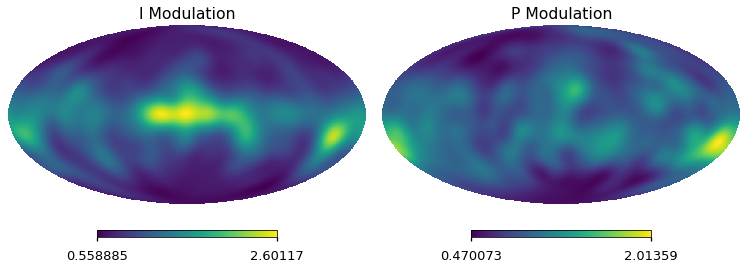
\includegraphics[width=2\columnwidth]{figures/mod_dust.png}\\
      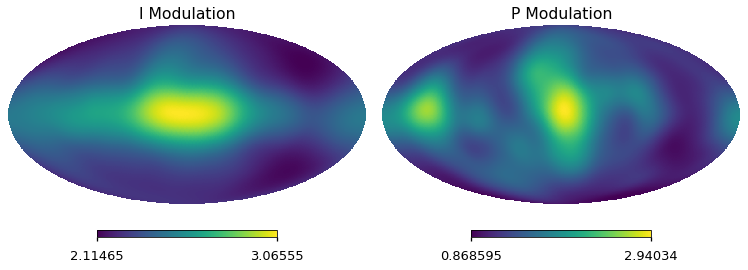
\includegraphics[width=2\columnwidth]{figures/mod_synch.png}\\
     \caption{Modulation maps $m_i$ and $m_p$ for (top) dust and  (bottom) synchrotron. }
     \label{fig:modulation_maps}
 \end{figure*}
 
\giuse{Table~\ref{tab:smallscale_par} presents the model parameters used to construct the modulation maps for dust and synchrotron emission, the chosen values are driven by  the angular resolution of the available templates.  For dust amplitude we consider  $\ell_1=100$ and $\ell_*=80$, whereas for synchrotron   $\ell_1=38$ and $\ell_*=36$. The second multipole scale, $\ell_2 =2000 (400)$ for dust (synchrotron) is chosen to be  in a range of scales where observations are currently lacking for both emissions.  } The modulation maps are illustrated in Figure~\ref{fig:modulation_maps}.

%Given that the intensity template has been estimated in a different way to the Q and U templates, we employ two different multipole scale cut-offs: $\ell=400$ and $100$, respectively. This further prevents the mixing of scales due to variable resolutions.

%\giuse{increasing at $\ell>40$ in the K-band spectra estimated by masking 80\% of the sky.  Therefore, we  adopt $\ell = 36$ as  cut-off multipole scale  for synchrotron.}

%The chosen cut-off multipole for $\beta_d$ and $T_d$ is the same as the one adopted for the intensity amplitude template, i.e., $\ell=400 $.

We do not intend for the above procedure to be useful for the inner Galactic plane, which has been imaged at high signal-to-noise ratio at relatively small scales. We thus do not apply the small-scale amplitude extrapolation to the $3\%$ of the sky in the Galactic plane as defined by the Planck \texttt{GAL097} mask\footnote{\texttt{HFI\_Mask\_GalPlane-apo2\_2048\_R2.00.fits}}.\giuse{ Instead we simply return the input data templates for the amplitudes in those regions. To ensure a smooth transition between template and synthesized small scales in the Galactic plane, we ensure the transition to be apodized  using a $5^\circ$ Gaussian taper.} This reflects our expectation that these maps are most useful for making physically motivated synthetic realizations of diffuse Galactic emission at high Galactic latitudes. %Moreover, the synthesis of small scales involves regions far from the Galactic plane, essentially outside in a region encoding 97\% of the sky. This is because, inside this area, the dust signal presents a very high SNR that small angular scales (e.g. $\sim20 $ arcmin ) are less affected by noise. We therefore decide to optimally exploit the state-of-art data on dust emission by employing the real small scales from observations nearby the Galactic plane.

% BH: To go through and ensure all is captured in the text above
%We first compute the $tt$, $ee$, and $bb$ power spectra from the dust template $i$, $q$, and $u$ maps and fit each with a power law $A\ell^{\gamma}$ in different multipole ranges depending on the native resolution of the map. Given that the intensity template has been estimated in a different way to the Q and U templates, we employ two different multipole scale cut-offs: $\ell=400$ and $100$, respectively. This further prevents the mixing of scales due to variable resolutions. Specifically, we employ $100 < \ell < 400$ for $tt$ and $30 < \ell < 110$ for $ee$ and $bb$. The spectral indices estimated from the fit are $\gamma = -1.29$, $-0.33$, and $-0.40$ for $tt$, $ee$, and $bb$, respectively.Adopting these values of $\gamma$ directly would lead to the $ee$ and $bb$ power exceeding $tt$ for large enough $\ell$ given the steeper index of the latter. {\bf Some words on why this is ok in principle but gives problems with polarization fraction in practice} We prevent this by adopting a common spectral index $\gamma = -1.29$ to extrapolate all three spectra to higher $\ell$. This choice is further motivated by the fact that the dust intensity template is provided at a higher resolution than the polarization ones, allowing to observe the dust specifics at higher detail with respect to the polarization data being more affected by noise and systematics. Although we are assuming that small scale polarized dust emission to be the same spectral index as the intensity one, this  is something that is physically intuitive and expected   from magneto-hydro dynamic simulations \citep[][]{Kim:2019}. We then generate $iqu$ maps encoding only small scales generated from the fit power law spectra and ranging from the pivot $\ell$-scale up to the multipole related to the desired pixel resolution scale of the dust map we want to simulate.  
%Since we want the small scales to be modulated by the amplitude of the dust emission at large scales, we apply two different modulations for the $i$ and for the $qu$ maps as they are convolved with different beam resolutions. We adopt  the $i$  map   smoothed at 5 deg as a template for both modulation maps.  We then identify a region encoding  low and intermediate Galactic latitudes by masking  all the pixels in the smoothed $i$ map  whose  value is $>4.5 \log ( \mu K )$.  The  intensity modulation is then constructed by performing two different normalization in the regions defined outside and inside  the mask. We use the \emph{MinMax} rescaling ranging   between $1$ and $2$ for the low-intermediate latitudes and between $0.1$ and $1$ for the high latitudes. For the polarization modulation map, we rescale similarly outside the mask between $0.1$ and $1$ but we saturate to   $1$  all the pixels  inside the low latitude region. Once the small scale maps are modulated, they are then co-added to the  low-pass filtered  $iqu$ maps (given the $\ell$-pivot scale) that encode  large scales only. Finally, the $iqu$ maps are transformed   back to the real $IQU$ maps  to perform the validation steps required to assess the quality of the maps. 

%\section{Dust and Synchrotron Model Templates} \label{sec:templates}
% In this section, we describe the data-driven templates used in the new models. %and comment on differences with previous PySM models.

\subsubsection{Dust Amplitude}\label{sec:dustamplitude}
The Planck~2015 component separation results in total intensity remain state of the art despite updates in polarization in the 2018 data release \citep{planck2016-l04}. Previous PySM models, e.g., \texttt{d0} and \texttt{d1}, employed the dust templates from the \texttt{Commander} component separation analysis \citep{planck2014-a11}. However, the model fitting employed in \citet{planck2014-a11} did not differentiate between Galactic dust emission and the Cosmic Infrared Background (CIB), and so the component separated dust maps retain CIB signal that should not be included in simulations of Galactic emission (see Section~\ref{sec:CIBcontamination} for detailed discussion). To address this issue, we instead use dust templates from analyses that separated Galactic dust emission from the CIB using the Generalized Needlet Internal Linear Combination (GNILC) algorithm \citep{Remazeilles:2011}. 

In total intensity we employ the Planck GNILC 2015 component separated map at $353$\,GHz \citep{planck2016-XLVIII}\footnote{\texttt{COM\_CompMap\_Dust-GNILC-F353\_2048\_R2.00.fits}}. This map has variable angular resolution, ranging from $21.8\arcmin$ up to $5\arcmin$ depending on the sky regions, which complicates its use in our analysis. Therefore, we reprocess the map as follows to a spatially uniform resolution of 21.8\arcmin. To do so, we first note that the map was synthesized from ten needlet (wavelet) maps of different, but spatially-uniform, resolution \citep[][Figure~A.2]{planck2016-l04}. We produce a map of uniform resolution by retaining only the first six needlet maps, which probe the dust intensity from the largest scales down to $21.8\arcmin$. This yields an $N_{\rm side} = 2048$ that reproduces the Planck GNILC 2015 dust intensity template at all scales $\geq 21.8$\arcmin. Finally, we subtract the CIB monopole of $0.13\, \text{MJy}\,\text{sr}^{-1}$ present in the map %\citep[][Section~2.2]{planck2016-l04}.
\citep[][Section~2.2]{planck2016-l11B}.

For the dust $Q$ and $U$ maps we employ the dust maps\footnote{\texttt{COM\_CompMap\_IQU-thermaldust-gnilc-varres\_2048\_R3.00.fits}} produced by the GNILC component separation from the third Planck release \citep{planck2016-l04,planck2016-l11B}. Unlike for the $I$ maps, we make use of the variable resolution maps to retain as much information as possible in the maps. The variable resolution $Q$ and $U$ maps have a resolution that varies much more smoothly across the sky than in the $I$ map [cite paper], making it more amenable to our methodology for adding small-scale fluctuations. The resolution of these maps ranges from $21.8\arcmin$ in the Galactic plane to $80\arcmin$ at high Galactic latitudes. The maps are pixellated at $N_{\rm side} = 2048$. 

To produce dust emission templates at a monochromatic frequency of 353\,GHz, we divide each of the $I$, $Q$, and $U$ maps by a factor of 1.098 to correct for the Planck bandpass \citep[][Table~2]{planck2016-l11A}.

\subsubsection{Synchrotron Amplitude}
Deriving a full-sky template for synchrotron emission in total intensity is challenging both for the paucity of low frequency surveys with full sky coverage and the difficulty in disentangling synchrotron emission from free-free emission and AME at frequencies above $\sim$10\,GHz. We follow \citet{Thorne:2017} in basing our template on the Haslam 408\,MHz survey with reprocessing \citep{Remazeilles:2015}. We rescale the 408\,MHz map of \cite{Remazeilles:2015} to 23\,GHz assuming a sky-constant power law $I_\nu \propto \nu^{-3.1}$. Finally, we smooth the resulting map to a resolution of $2^\circ$.

Constructing a synchrotron template in polarization is somewhat easier than total intensity because both free-free emission and AME have very low levels of polarization. Thus, we employ the WMAP K-band (23\,GHz) $Q$ and $U$ maps directly as our templates. As with the $I$ map, we smooth the $Q$ and $U$ templates to a resolution of $2^\circ$.

% BH: Did we do anything about bandpasses?

\subsection{Small Scale Fluctuations in Spectral Parameters}

\subsubsection{Methods Overview}
\begin{table}
    \centering
    \begin{tabular}{lcc}
    \toprule 
   &   $ \ell_1   $    &$\alpha$  \\
   \midrule  
   $\beta_d$ & 400 & 0.04 \\ 
   $T_d$  &  400  & -0.47\\
    \midrule 
    $\beta_s$ & 38 & -0.61\\
    $c_s$ & 38 &  -0.61  \\ 
   \bottomrule
    \end{tabular}
    \caption{Spectral indices adopted for synthesizing  small scales in the spectral parameters of dust and synchrotron models. }
    \label{tab:smallscale_specpar}
\end{table}

Just as a map of Galactic emission at a single frequency is expected to have fluctuations at smaller angular scales than have been measured, maps of parameters governing its frequency dependence should also have small-scale fluctuations. We therefore introduce small scale fluctuations to our spectral parameter template maps in a way analogous to the amplitude template maps. This more realistically captures the complexity of small-scale Galactic emission.
%\giuse{ Indeed most of the previous models  did not include fluctuations beyond what was already captured by the templates \citep{Thorne:2017}.}

As there is no sense of polarization in the spectral parameter maps, we do not work within the polarization fraction tensor framework but rather with standard power spectra. Given a template map $\mathcal{T}$ of some spectral parameter $\beta$, we first fit the power spectrum of $\mathcal{T}$ with a power law $C_\ell \propto \ell^\alpha$ over a range of scales where it is well measured, up to some multipole $\ell_1$. We then generate a map of small scale fluctuations using the power law fit. We multiply the resulting map by a modulation map in analogy with the amplitude modulations described in Section~X. Finally, we combine the template map with the synthesized small scales using the filter function in Equation~X.

The application of this procedure to the dust and synchrotron spectral parameters is described in the following sections. The adopted fit parameters for each spectral parameter are listed in Table~\ref{tab:smallscale_specpar}.

\subsubsection{Dust Spectral Parameters}\label{subsec:dust_spec_params}
As described in Section~\ref{sec:dustamplitude}, the dust emission in all models developed here is governed by the spectral parameters $\beta_d$ and $T_d$. For the $\beta_d$ and $T_d$ template maps, we employ the $\beta_d$ and $T_d$ maps\footnote{ \texttt{COM\_CompMap\_Dust-GNILC-Model-Spectral-Index\_2048\_R2.00.fits}, \texttt{COM\_CompMap\_Dust-GNILC-Model-Temperature\_2048\_R2.00.fits}} derived from 2015 Planck GNILC component separation analysis. These maps benefit from lower CIB residuals than the \texttt{Commander} $\beta_d$ and $T_d$ as the methodology employed both spatial and spectral information to disentangle the CIB contribution to the total emission.
%However, the estimate of $\beta_d$ and $T_d$ is highly degenerate making the maps at small angular scales ($<21.8^\prime$) are contaminated by artifacts due to noise and calibration errors. 

We fit the power spectra of the $\beta_d$ and $T_d$ template maps over the multipole ranges $200 < \ell < 400$ and $100 < \ell < 400$, respectively. We find that $\alpha_{\beta_d}= 0.04$ and $\alpha_{T_d} = -0.47$ over this range, both flatter than the $\alpha_{tt} = -0.80$ found for the dust amplitude. The adopted pivot multipole $\ell_1$ is larger than that used for dust amplitudes (see Table~\ref{tab:smallscale_par}) since the template maps employed here are derived from intensity-only data rather than a combination of total and polarized intensity. Thus, they remain signal-dominated at $\sim$4 times smaller angular scales.

We construct the modulation map from the GNILC $I$ map smoothed to a resolution of $5^\circ$. We apply a linear renormalization such that the (now dimensionless) pixel values in the map range from 0.1 to 2. %BH The text below makes me think that pixels in the I map above and below a certain threshold were ignored in this process rather than taking the literal min and max values of the map

%\giuse{ Also in this case, we   employ a modulation map for the $\beta_d$ and $T_d$ synthetic small scales.   The modulation template is derived from $I$ GNILC amplitude map, smoothed  at 5 deg and \emph{min-max} normalized   from $0.1$ and $2$. The latter step is needed as we expect the modulation map to be dimensionless and  the extreme values have been  empirically identified as the best choice to preserve the range of variation observed in   $\beta_d$ and $T_d$ at both low and intermediate Galactic latitudes. } 

% BH: This is potentially important, but probably belongs in the validation section
%However,  we do not expect small scales generated with the spectral parameter maps  to dominate when rescaling maps at frequencies other than the reference one (353 GHz). \giuse{This is mainly granted by the fact that amplitude small scales are few orders of magnitude larger than the ones injected in the  spectral parameter, in the whole range of reliability of the PySM models, e.g. 10-1000 GHz.}
 
\subsubsection{Synchrotron Spectral Parameters}\label{sec:beta_s}
As described in Section~X, the synchrotron emission in all models developed here is governed by the spectral parameters $\beta_s$ and $c_s$. To build the large scale template for the spatial variation of the synchrotron spectral index $\beta_s$, we begin with the full-sky $\beta_s$ map obtained by combining the Haslam map in total intensity at 408\,MHz \citep{Remazeilles:2015} and WMAP K-band data \citep{Miville-Deschenes:2008}. The map has an angular resolution of about $7^{\circ}$ and was employed by previous PySM synchrotron models \citep{Thorne:2017}.

Incorporating newer constraints on synchrotron emission at 2.3\,GHz from S-PASS, \citet{Krachmalnicoff:2018} determined that this $\beta_s$ map underestimates the true level of spatial variations in $\beta_s$ across the Southern Galactic Hemisphere. Thus, we follow \citet{Krachmalnicoff:2018} and rescale the $\beta_s$ map by first subtracting its mean value, multiplying the resulting map by a factor of $1.572$, and then adding back the mean value.

We next fit a power-law to the power spectrum of this new template map over the multipole range $2<\ell<38$, finding $\alpha_{\beta_s}=-0.61$ then construct a map from this power spectrum extrapolated to high multipoles. We next construct a modulation map by taking the Haslam 408\,GHz $I$ map, smoothing to $5^\circ$ resolution, then renormalizing the map through a linear transformation such that the (dimensionless) pixel values range from 0.1--2. As with the dust spectral parameter maps (see Section~\ref{subsec:beta_d}), we combine this high-$\ell$ map with the low-$\ell$ template following the filter function of Equation~X. %BH: I don't understand the following sentence: Even in this case, the extreme of rescaling ensure the excursion range  of observed synchrotron spectral index.
 
For the synchrotron curvature parameter $c_s$, there are no readily available template maps. The existing \texttt{s3} model implements curvature as a sky-constant $c_s = -0.052$, consistent with the measurements from ARCADE \citep[$c_s=-0.052 \pm 0.005$][]{Kogut:2012}. As an attempt to model a reasonable range of spatial variability, we assume that fluctuations in the value of $c_s$ follow the synchrotron intensity at large angular scales. Specifically, we start from the Haslam map 408\,MHz $I$ map smoothed to a resolution of $5 \deg$, which we then rescale with a linear transformation such that the minimum and maximum pixel values are  $-0.0517$ and $0.0054$, respectively, corresponding to the range of $c_s$ measurements from ARCADE \citep{Kogut:2012}. The resulting $c_s$ map has a mean and standard deviation of $-0.0517$ and $0.0054$, respectively. 

% BH: If this was done, it needs to be described quantitatively with reference to the relevant equations
%Finally, both the $\beta_s$ and the $c_s$ templates are low pass filtered with $\ell=36$ to minimize artifacts from noise and the large beamsize.

To extend our $c_s$ map to smaller angular scales $\ell > 36$, we first generate a map of Gaussian random fluctuations with the same power law index as the $\beta_s$ map, i.e., $\alpha _{c_s}=\alpha _{\beta_s} = -0.61$. We modulate the resulting map with the same modulation map as used for $\beta_s$ and combine this high-$\ell$ map with the low-$\ell$ template following the filter function of Equation~X.
%Small  scales at multipoles $\ell>36$  are therefore  included   assuming them to follow  the same power law as  the $\beta_s$ ones,  i.e. $\alpha _{c_s}=\alpha _{\beta_s} = -0.61$, and that are  modulated with the exact same modulation map as the one we  adopted for $\beta_s$.

\subsection{New Model Summary}
Explain d9, d10, d11, s5, s6, s7 here

\section{Other Models Implemented in PySM} \label{sec:other_models}

\subsection{Dust Layer Model} \label{sec:layers}
%Evidence for variation of Galactic foreground emission laws as a function of frequency across the sky implies that emission laws must vary along the line of sight. As a consequence, we anticipate that dust emission, if locally matching a modified blackbody in the form of Equation~\ref{eq:dust-emission-law}, is seen by an observer as a superposition (an integral along the line of sight) of modified blackbodies -- which is not a modified blackbody. In addition, if along the line of sight different line elements emit polarized radiation with different polarization angles, the frequency scaling should vary between $I$, $Q$ and $U$ \citep{2015MNRAS.451L..90T}.
\giuse{To model the complexity of multiple layers of dust along the line of sight, we based our  PySM~3 implementation  on the approach of \cite{Martinez-Solaeche:2018} in the PSM software\footnote{See version 2.3.3 \url{https://apc.u-paris.fr/~delabrou/PSM/psm.html}.}. }

The PSM has been run to produce six maps of dust emission at 353~GHz (intensity and polarization, for a total of 18 HEALPix maps at {\tt nside=2048}), and six maps of dust spectral index $\beta_d$ and dust temperature $T_d$, also at {\tt nside=2048}, following the approach described in \cite{Martinez-Solaeche:2018}. The PySM software uses these maps as inputs, and generates the dust Stokes parameters maps as:
\begin{equation}
    S_\nu(p) = \sum_{k=1}^6 S^{(k)}_{\nu_{\rm ref}}(p)
    \left( \frac{\nu}{\nu_{\rm ref}} \right)^{\beta^{(k)}_d(p)}
    \frac{B_\nu(T^{(k)}_d(p))}{B_{\nu_{\rm ref}}(T^{(k)}_d(p))},
\end{equation}
where $S_\nu(p)$ stands for any of the three Stokes parameters of interest, $I$, $Q$ and $U$, at frequency $\nu$ and in pixel $p$, and superscripts ${(k)}$ indicate the layer, from 1 to 6.

\giuse{ We remark, that in the implementation used here , the 353~GHz templates for the six emission layers are slightly different from those of \cite{Martinez-Solaeche:2018} as we employ more recent Planck data products. Large scale polarized emission maps are the GNILC maps obtained in \cite{planck2016-l04} using the method developed by \cite{Remazeilles:2011}. These are complemented by small scale realizations with scale dependence matching the $T$, $E$ and $B$ dust spectra measured in \cite{planck2016-l11A}, modulated by the large scale local intensity and polarized intensity level. This results into effectively  filter out  some of the real small scale power in  intensity and polarization dust maps, and it replaces it with random fluctuations. Thus we expect departures on the non-Gaussian and non-stationary properties of real dust emission.  We devote a future work the improvement of statistical properties of the generated of small scale fluctuations. }

% \item Methodology, especially the connection between MKD and what we implement in PySM. What capabilities of PySM can we exploit to extend MKD?
%  \item Comments on any numerical trickiness, e.g., p > 1

\subsection{CO Emission}

PySM3 employs models of Carbon Monoxide (CO) emission  of  the first three CO rotational lines: $J = 1\rightarrow0, 2\rightarrow1$, and $3\rightarrow2$ transitions at 115.3, 230.6, and 345.8\,GHz, respectively. We adopted  the CO $J = 1\rightarrow0$ \texttt{Type-1} map\footnote{\url{HFI_CompMap_CO-Type1_2048_R2.00.fits}} released by \citet{2014A&A...571A..13P}.  This CO map is obtained exploiting the mismatches in the detector bandpass to recover the CO from the CMB and the other Galactic foregrounds, with the MILCA component separation algorithm.  
 
%Although the \texttt{Type-1} maps suffer of a lower SNR with respect to the other maps they are less affected by Galactic foreground residuals, as they encode information coming solely from the 100 GHz \emph{Planck} detectors. 
Moreover, being the  CO map has been released at the nominal resolution (10\arcmin) we convolve it with a 1$^\circ$ gaussian beam to further lower the noise contamination  especially at intermediate and high Galactic latitudes.

CO line emission can be linearly polarized via the Goldreich-Kylafis effect \citep{Goldreich:1981, Crutcher:2012}.  As CO polarization surveys are hard to be realized,  mainly due to the intrinsically low degree of polarization and the long integration time required to achieve a significant detection,  so far the approach has been to model it assuming an, albeit small, degree of polarization. \citet{Puglisi:2017} presented a model to simulate the polarized emission of CO lines in molecular clouds at high Galactic latitudes by considering the 3D spatial distribution of CO in the Galaxy. The model   successfully reproduced not only the angular power spectrum of the observed Planck  CO intensity maps \citep{planck2013-p03a},  but also the intensity profile  in longitude bins at low Galactic latitudes.  Given the lack of observational constraints, the model assumed a strong correlation between the CO polarization and the polarized galactic dust emission to forecast the amplitude of CO polarized emission. 

 We, thus,  propose  3  models of CO emission defined as follows: 
\begin{itemize}
    \item {\bf\texttt{co1}:} unpolarized emission using  the Planck templates derived from  CO $J:1\rightarrow0$ Type 1 intensity   maps \citep{planck2013-p03a}. To reduce noise contamination, we downgrade the resolution of the maps at 1 deg and repixelized to Healpix \texttt{nside=512}. 
      \item {\bf\texttt{co2}:} model for both unpolarized and polarized emission, with fractional polarization a free parameter set by the user (default $\Pi = 0.1 \%$). This model employs the same intensity templates used in  {\bf\texttt{co1}}.  Stokes $Q$ and $U$ CO maps are modeled following \citet[eqs. (12) and (13) of]{Puglisi:2017}, employing  depolarization  and polarization angle  templates derived from   Planck thermal dust maps \citep{planck2014-a12}. 
        \item {\bf\texttt{co3}:}  model for both unpolarized and polarized emission, as defined in {\bf\texttt{co2}}. This model further accounts for the emission from high-Galactic latitude clouds simulated with the procedure outlined in \citet{Puglisi:2017}.
\end{itemize}
 


\section{Validation and Characterization of Models} \label{sec:validation}

In this section, we validate the foreground models developed in Section~\ref{sec:small_scales}.
%
%\giuse{We firstly show a comparison in Section~\ref{subsec:maps} at the map level of the new models, to visually appreciate the differences between with the templates and the previous PySM models.} 
\jd{In Section~\ref{subsec:maps}, we show map comparisons to visually appreciate the differences between the various PySM models and real-sky observations.}
%
In Section~\ref{sec:dust_validation} we demonstrate that the two-point statistics of the stochastic small scales are properly modulated for different regions of sky defined by Galactic masks of varying size. We also assess the properties of our dust model in the small patch of sky observed by the BICEP / Keck telescopes and the South Pole Telescope.  
%
%\sg{In Section~\ref{sec:sync_validation} we compare the power spectra of different synchrotron models with BeyondPlanck synchrotron map for temperature, and LFI 30 GHz for polarization. We find a reasonable agreement between the data and our models for different fraction of the Galactic synchrotron signal masked.} 
\jd{In Section~\ref{sec:sync_validation}, we compare the power spectra of different PySM synchrotron models with the synchrotron map from the BeyondPlanck analysis for Intensity, and with the LFI 30 GHz observations for polarization. We find a reasonable agreement between the data and our models for different fraction of the Galactic synchrotron signal masked.}
%
\giuse{/bf describe also section on decorrelation}. In Section~\ref{sec:nongaussianity}, we assess the level of non-Gaussianity introduced by the log polarization tensor formalism, and compare this to the case of a purely Gaussian small scale model which has been modulated by a Galactic template. 


\subsection{Maps}\label{subsec:maps}

\jd{PySM models are based on noisy observations of Galactic foreground amplitude maps, complemented in some cases by randomly generated small-scale features (sec.~\ref{sec:small_scales}). Maps of frequency scaling parameters also comprise randomly generated fluctuations, the generation of which is different for the various models. It is important to check to which extent model maps match with observations in the frequency range of interest. In this first step of validation of the PySM foreground models, we compare, for the different foreground models considered here, maps generated using the PySM and actual observations in the frequency range of interest.}\textcolor{red}{[What frequencies do we want to cover? I suggest at least 23~GHz--353~GHz, but this does not fully cover the frequency range of CMB-S4 and LiteBIRD]}
Specifically, we compare observations the Planck third data release PR3 \cite{planck2016-l03} and PySM dust models \dnine{}, {\tt d11}, {\tt d12} models at the map level. We study how the modeled intensity $I$ and polarized intensity $P = \sqrt{U^2 + Q^2}$ compare to the observations on three selected $16.7^\circ \times 16.7^\circ$ patches of the sky, at 353~GHz. Here, we focus on two local patches: close to the Galactic plane ($[l,b] =[180^\circ,-10^\circ]$) and, centered on the Bicep / Keck field ($[l,b] =[318^\circ,-61^\circ]$).
We integrate the dust models within the Planck passband (\cite{planck2013-p03d})\footnote{\url{http://pla.esac.esa.int/pla/aio/product-action?MAP.MAP_ID=HFI_RIMO_R3.00.fits}}, to enable a more straightforward comparison. For the comparison of dust intensity maps, we subtract a Wiener-filtered CMB temperature anisotropies map from SMICA and also adjust (setting to zero) the zero level of the PR3 data and of the simulated maps over a small region of very low dust emission, totaling a sky fraction of 2.5\%.
%to that of the simulated map over regions of faint dust intensity on the sky.
\jd{This readjustment is slightly different for the three dust models and the data considered (i.e. the zero level is not exactly the same in all the maps).} We compute the mean of the intensity in the regions considered for the three dust models and data and then subtract this quantity from the dust intensity of each model and data. The mask used to adjust the zero levels is shown in figure \ref{fig:mask_zero_lvl_int}. 
These corrections are not required for comparing polarization data. 
%PR3: 13.97uKcmb
%d9: 14.46uKcmb
%d11: 14.59uKcmb
%d12: 6.41uKcmb
%note: JD - there is considerable uncertainty on the zero level of the maps (if I got my calculations right, the CIB monopole at 353GHz is of the order of 300uKcmb, and is not known with 5% accuracy -- the difference between models based on FIRAS is more like 10-20%)


\begin{figure}[ht!]
    \centering
    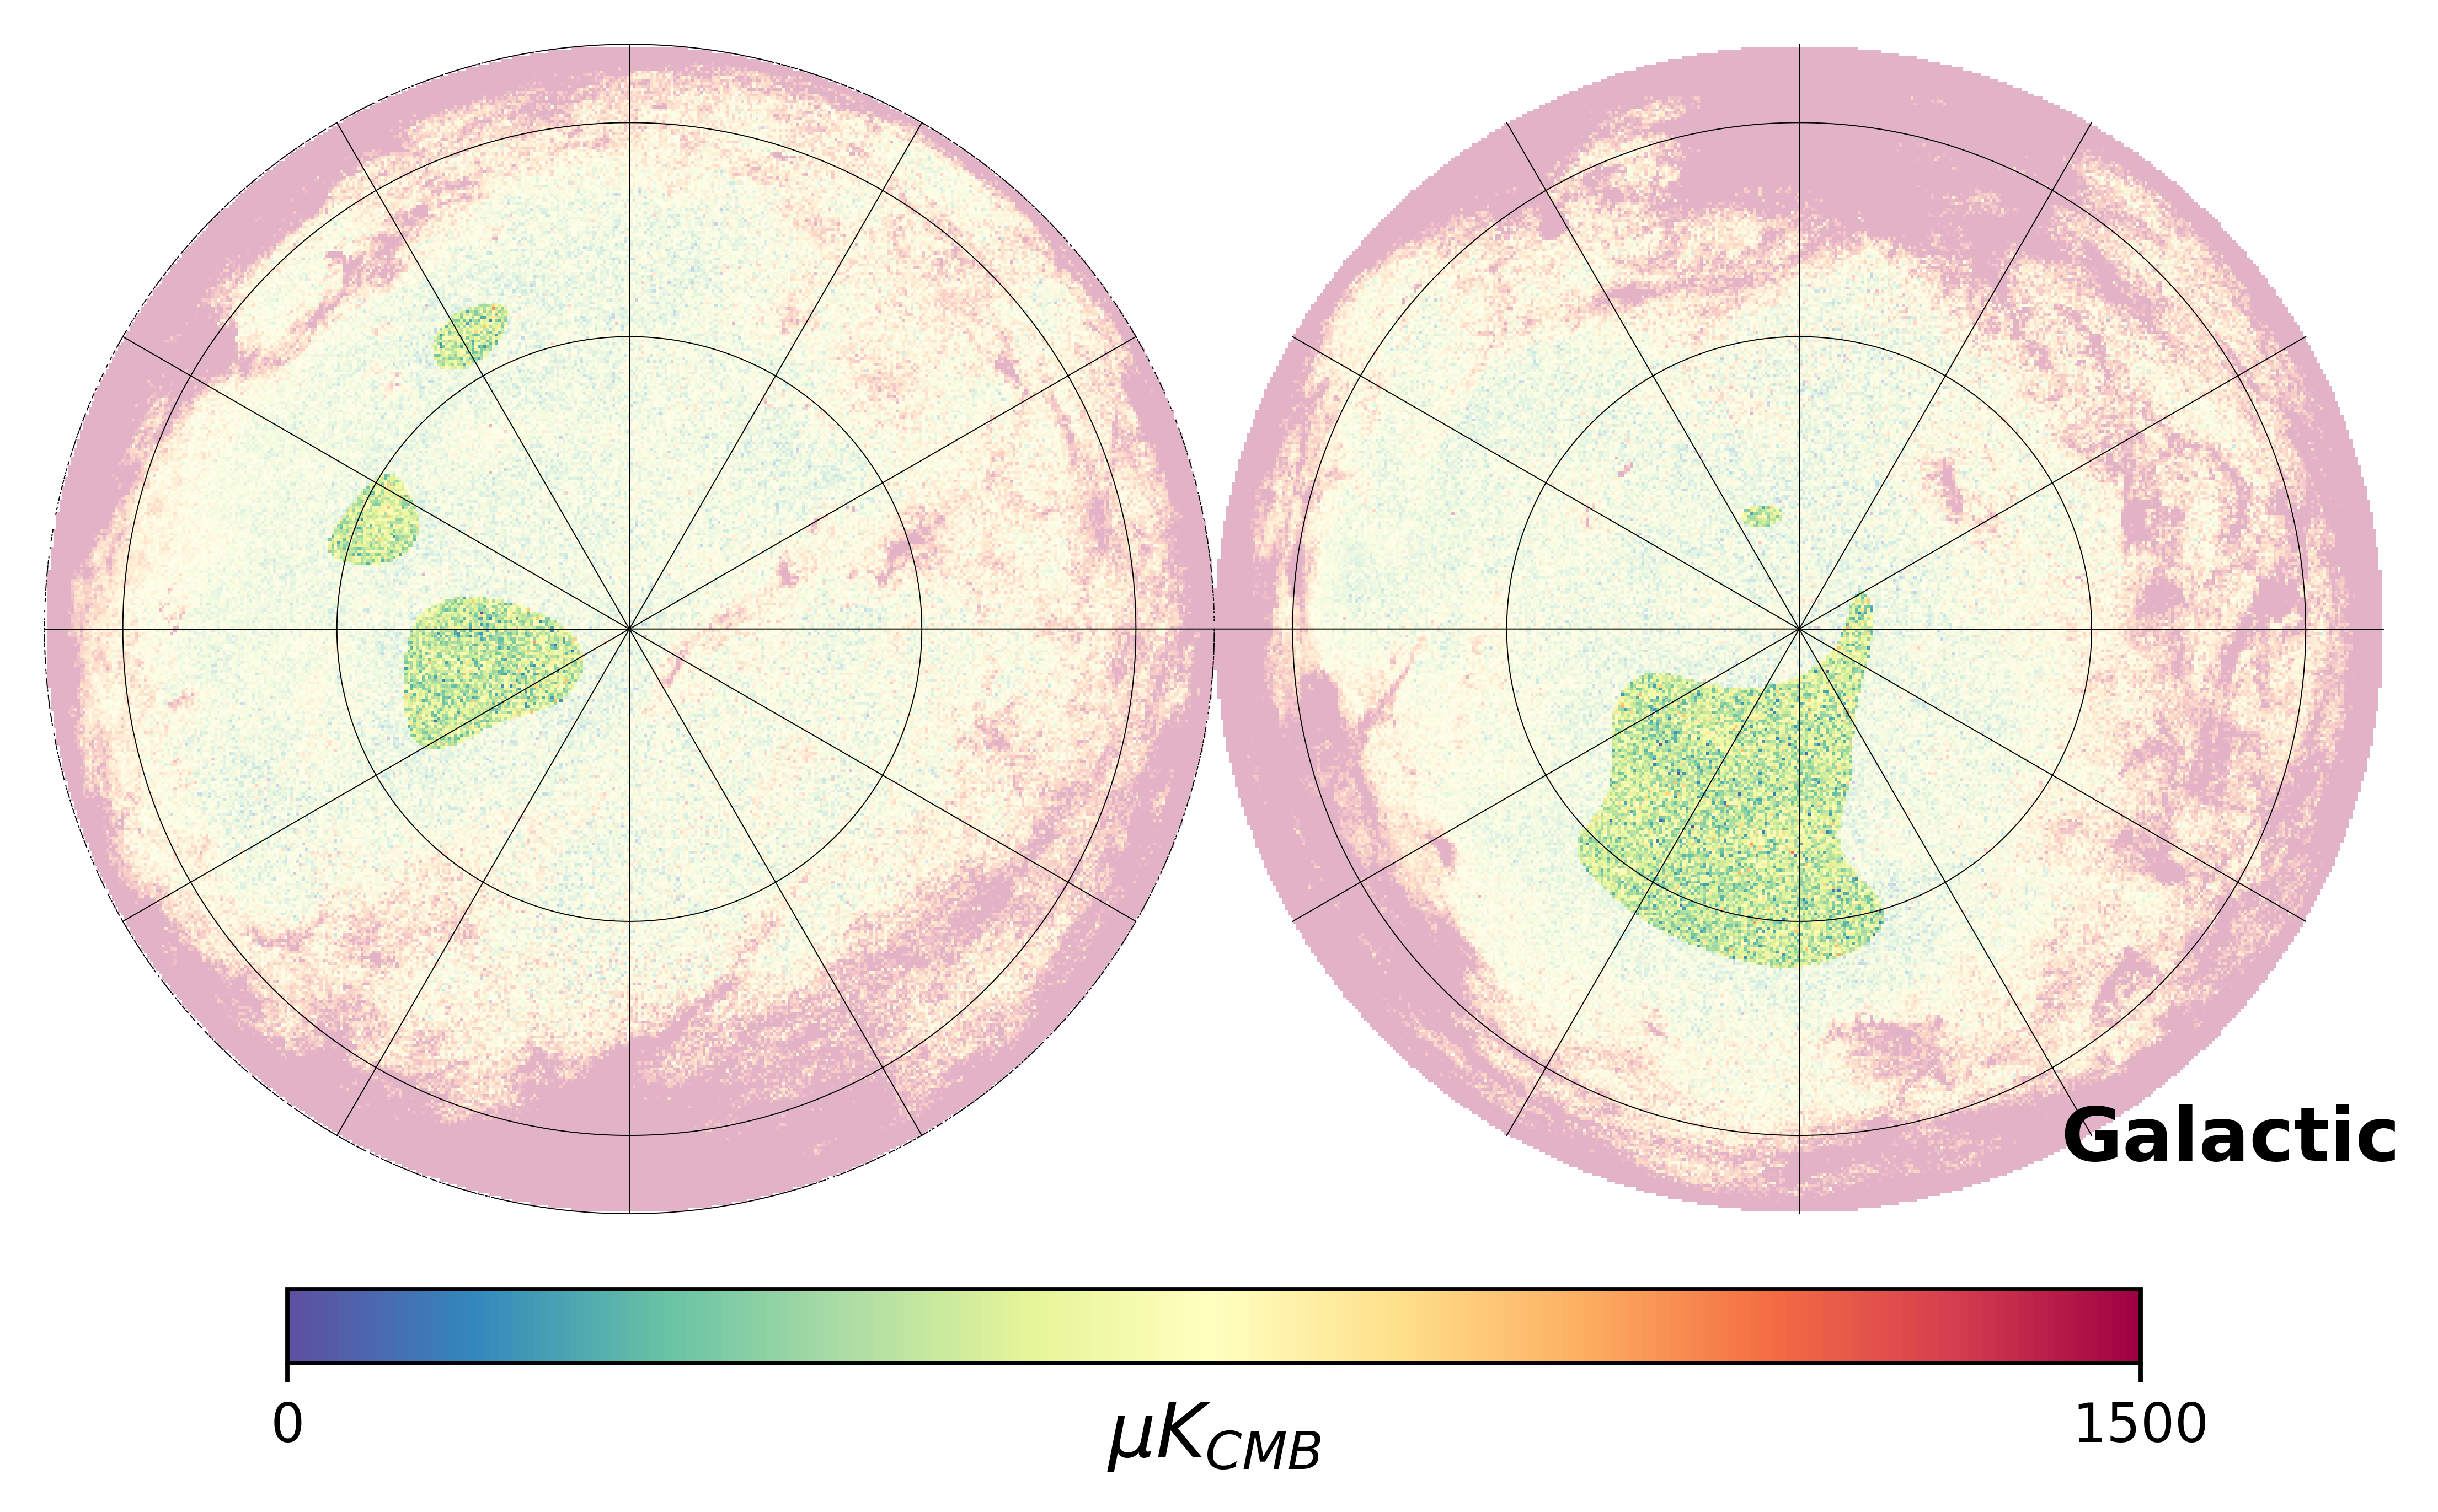
\includegraphics[width=0.48\textwidth]{figures/mask_intxPR3_zero_lvl.png}
    \caption{Mask $\times$ PR3 intensity used to estimate the zero level of PR3 intensity. This mask is obtained by thresholding the intensity of the smoothed PR3 intensity to preserve only the regions where the dust is very low, to estimate the zero-level of the data and models.}
    \label{fig:mask_zero_lvl_int}
\end{figure}

\begin{figure}[ht!]
    \centering
    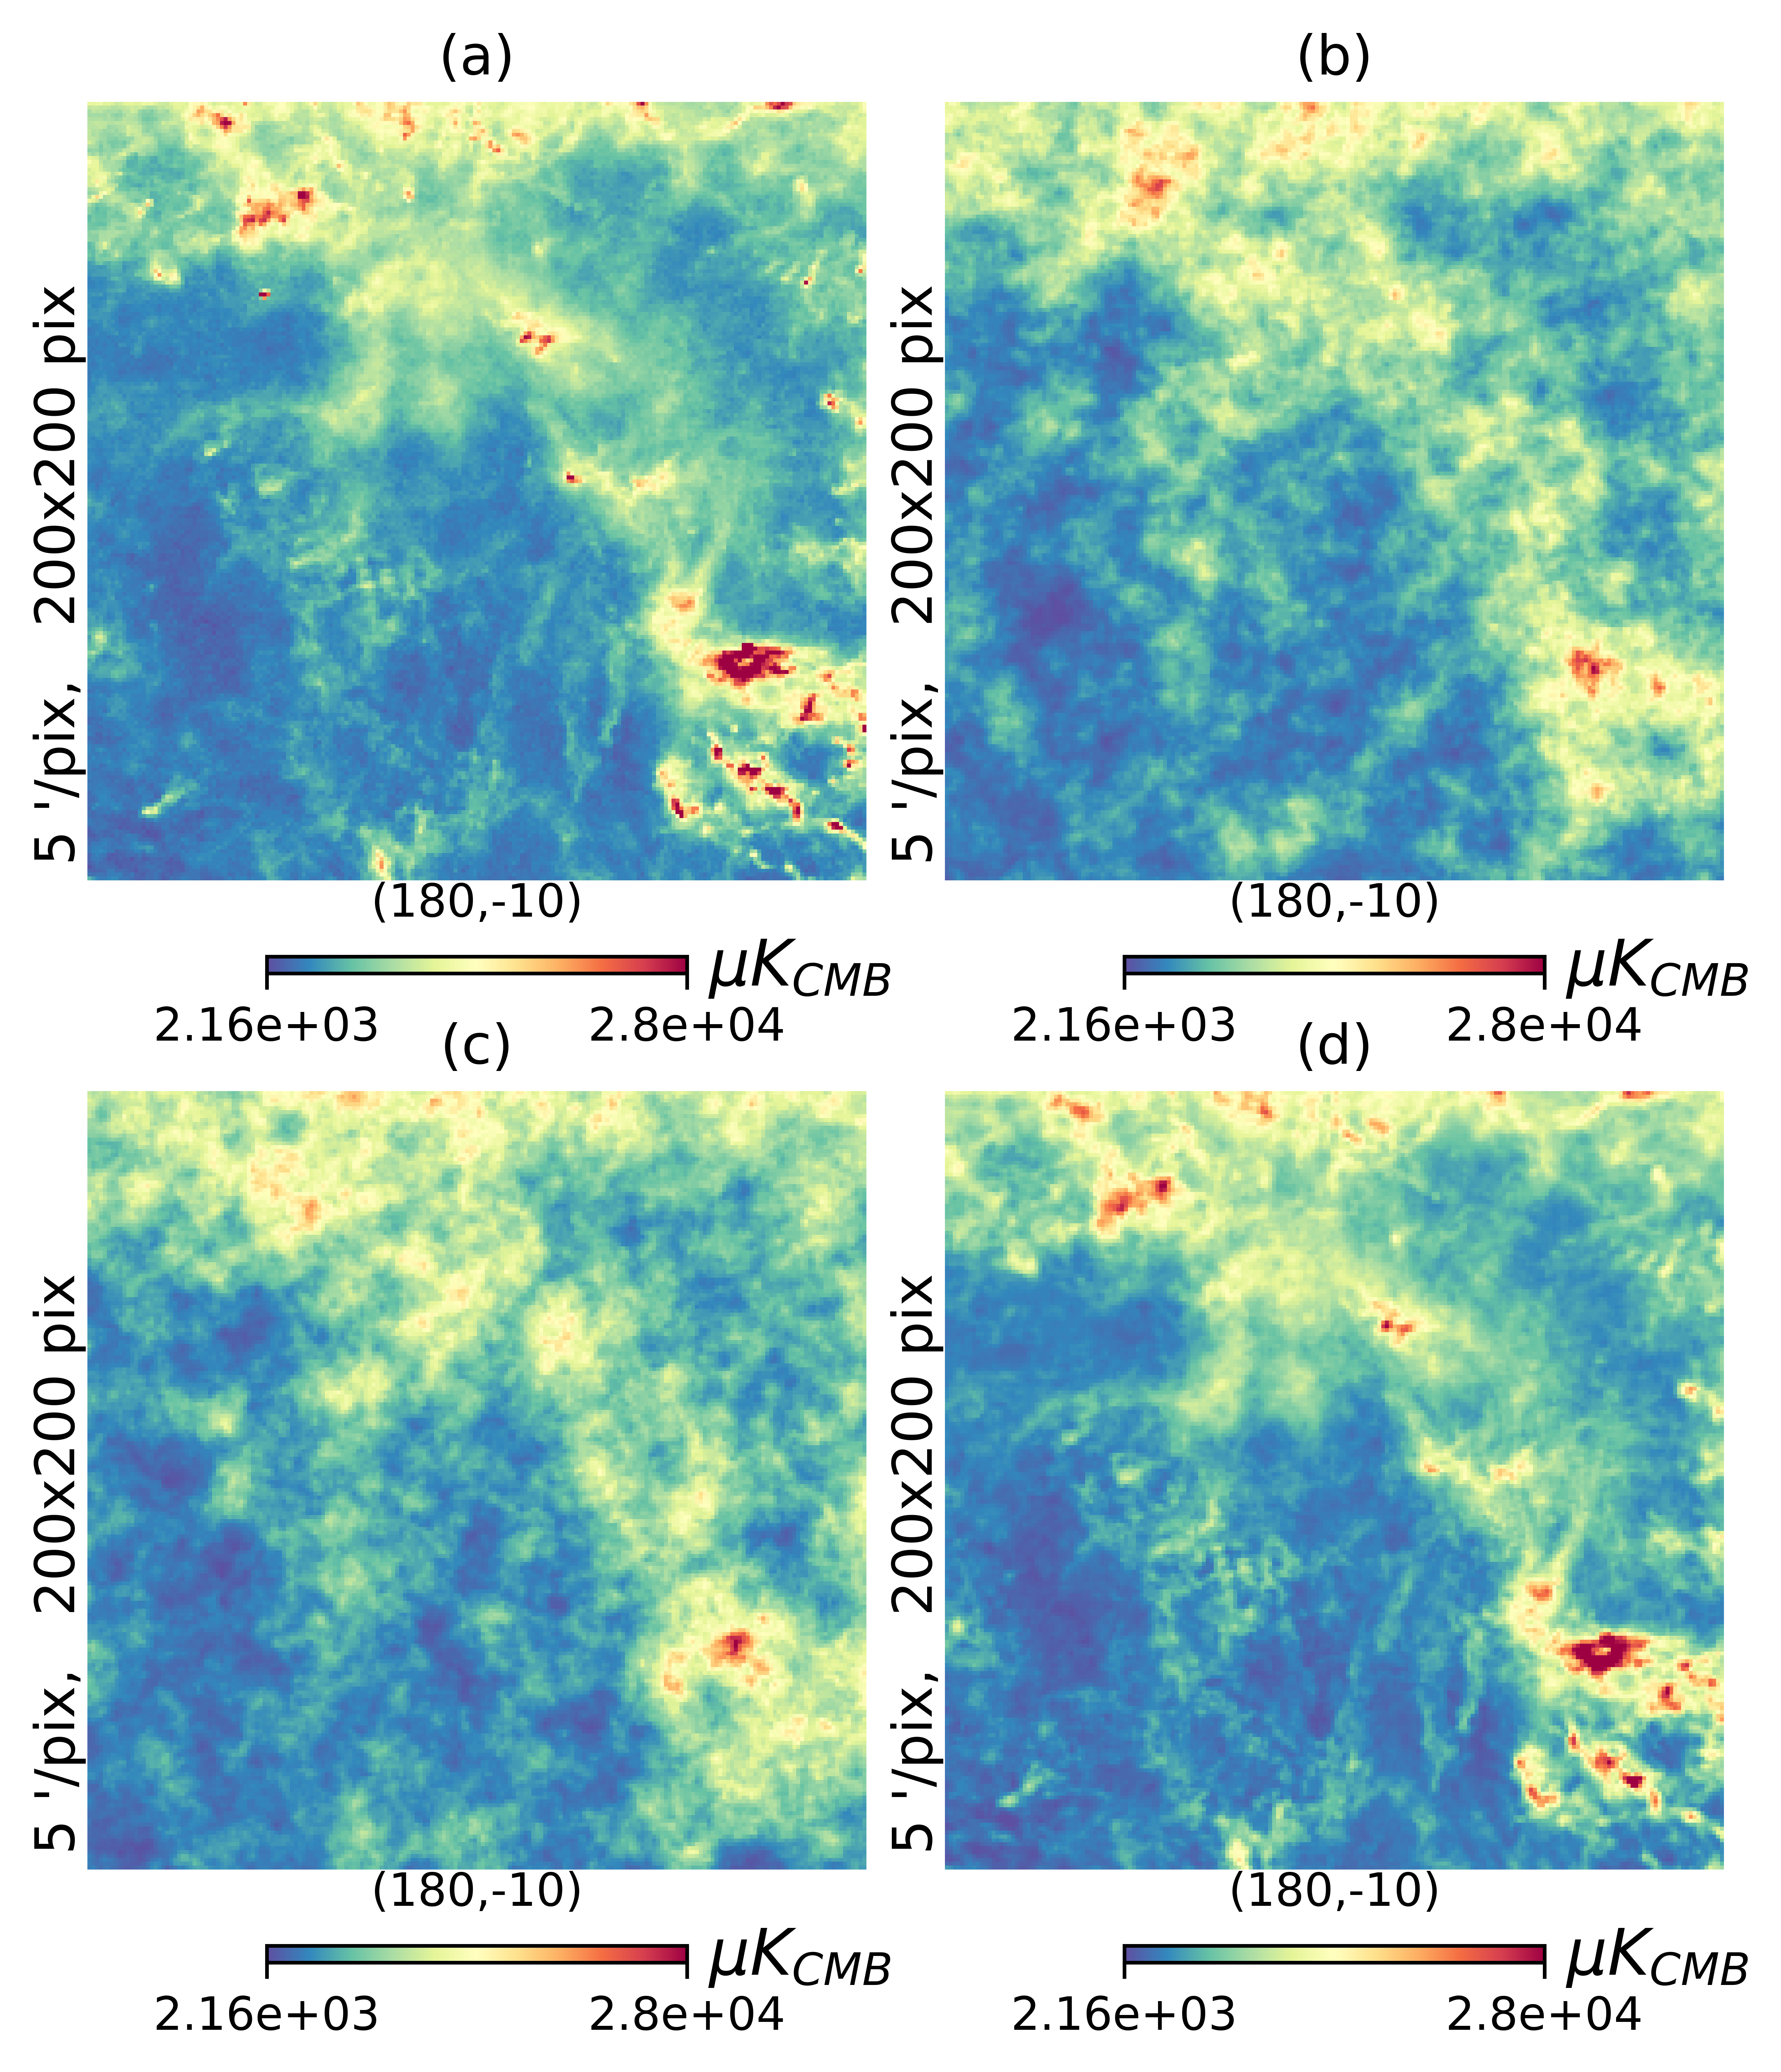
\includegraphics[width=0.48\textwidth]{figures/gal_plane_non_smooth_wo_zero_lvl.png}
\caption{Dust intensity at 353GHz at [l = 180, b = -10] with an angular resolution of $4.94\arcmin$: (a) PR3 (b) d9 (c) d11 (d) d12. The gap between the white lines represents $4^{\circ}$. }    
\label{fig:353_int_gal_plane}
\end{figure}
% \begin{figure}
%     \centering
%     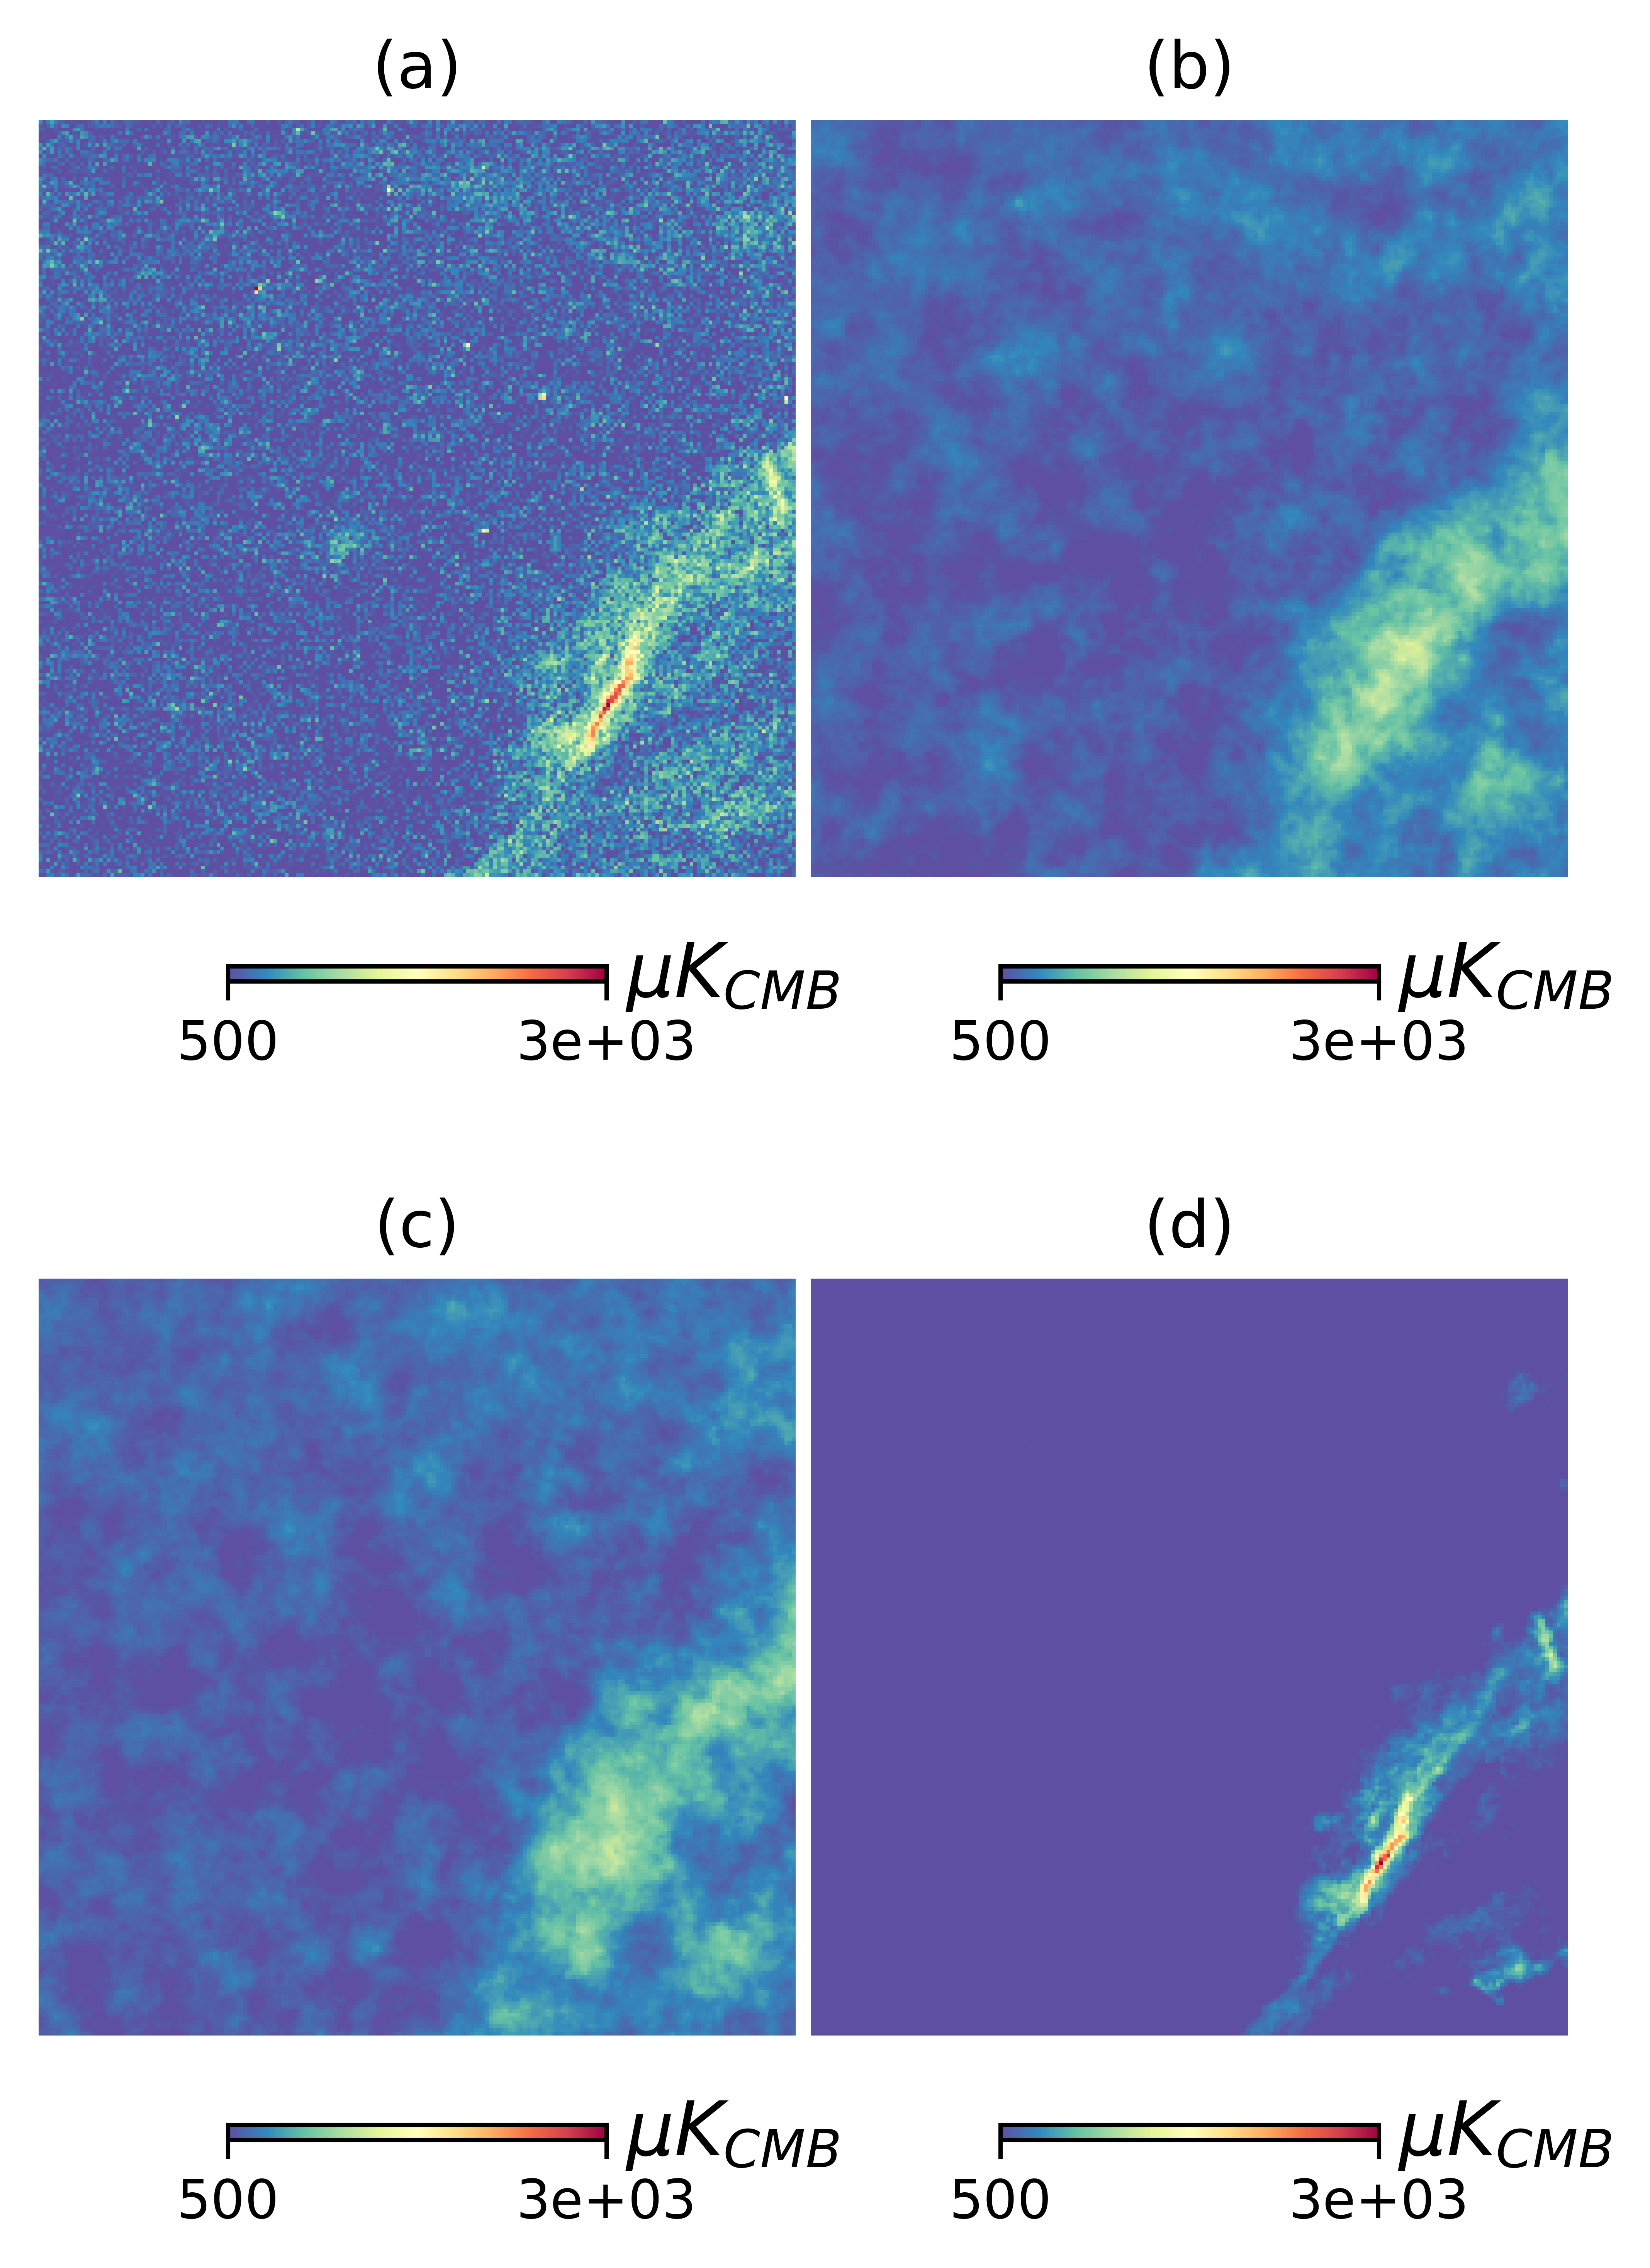
\includegraphics[scale = 0.6]{figures/NGP_non_smooth_wo_zero_lvl.png}
%     \caption{Dust intensity at 353GHz centered at [l = 0, b = 90]: (a) PR3 (b) d9 (c) d11 (d) d12}
%     \label{fig:353_int_NP}
% \end{figure}
\begin{figure}[ht!]
    \centering
    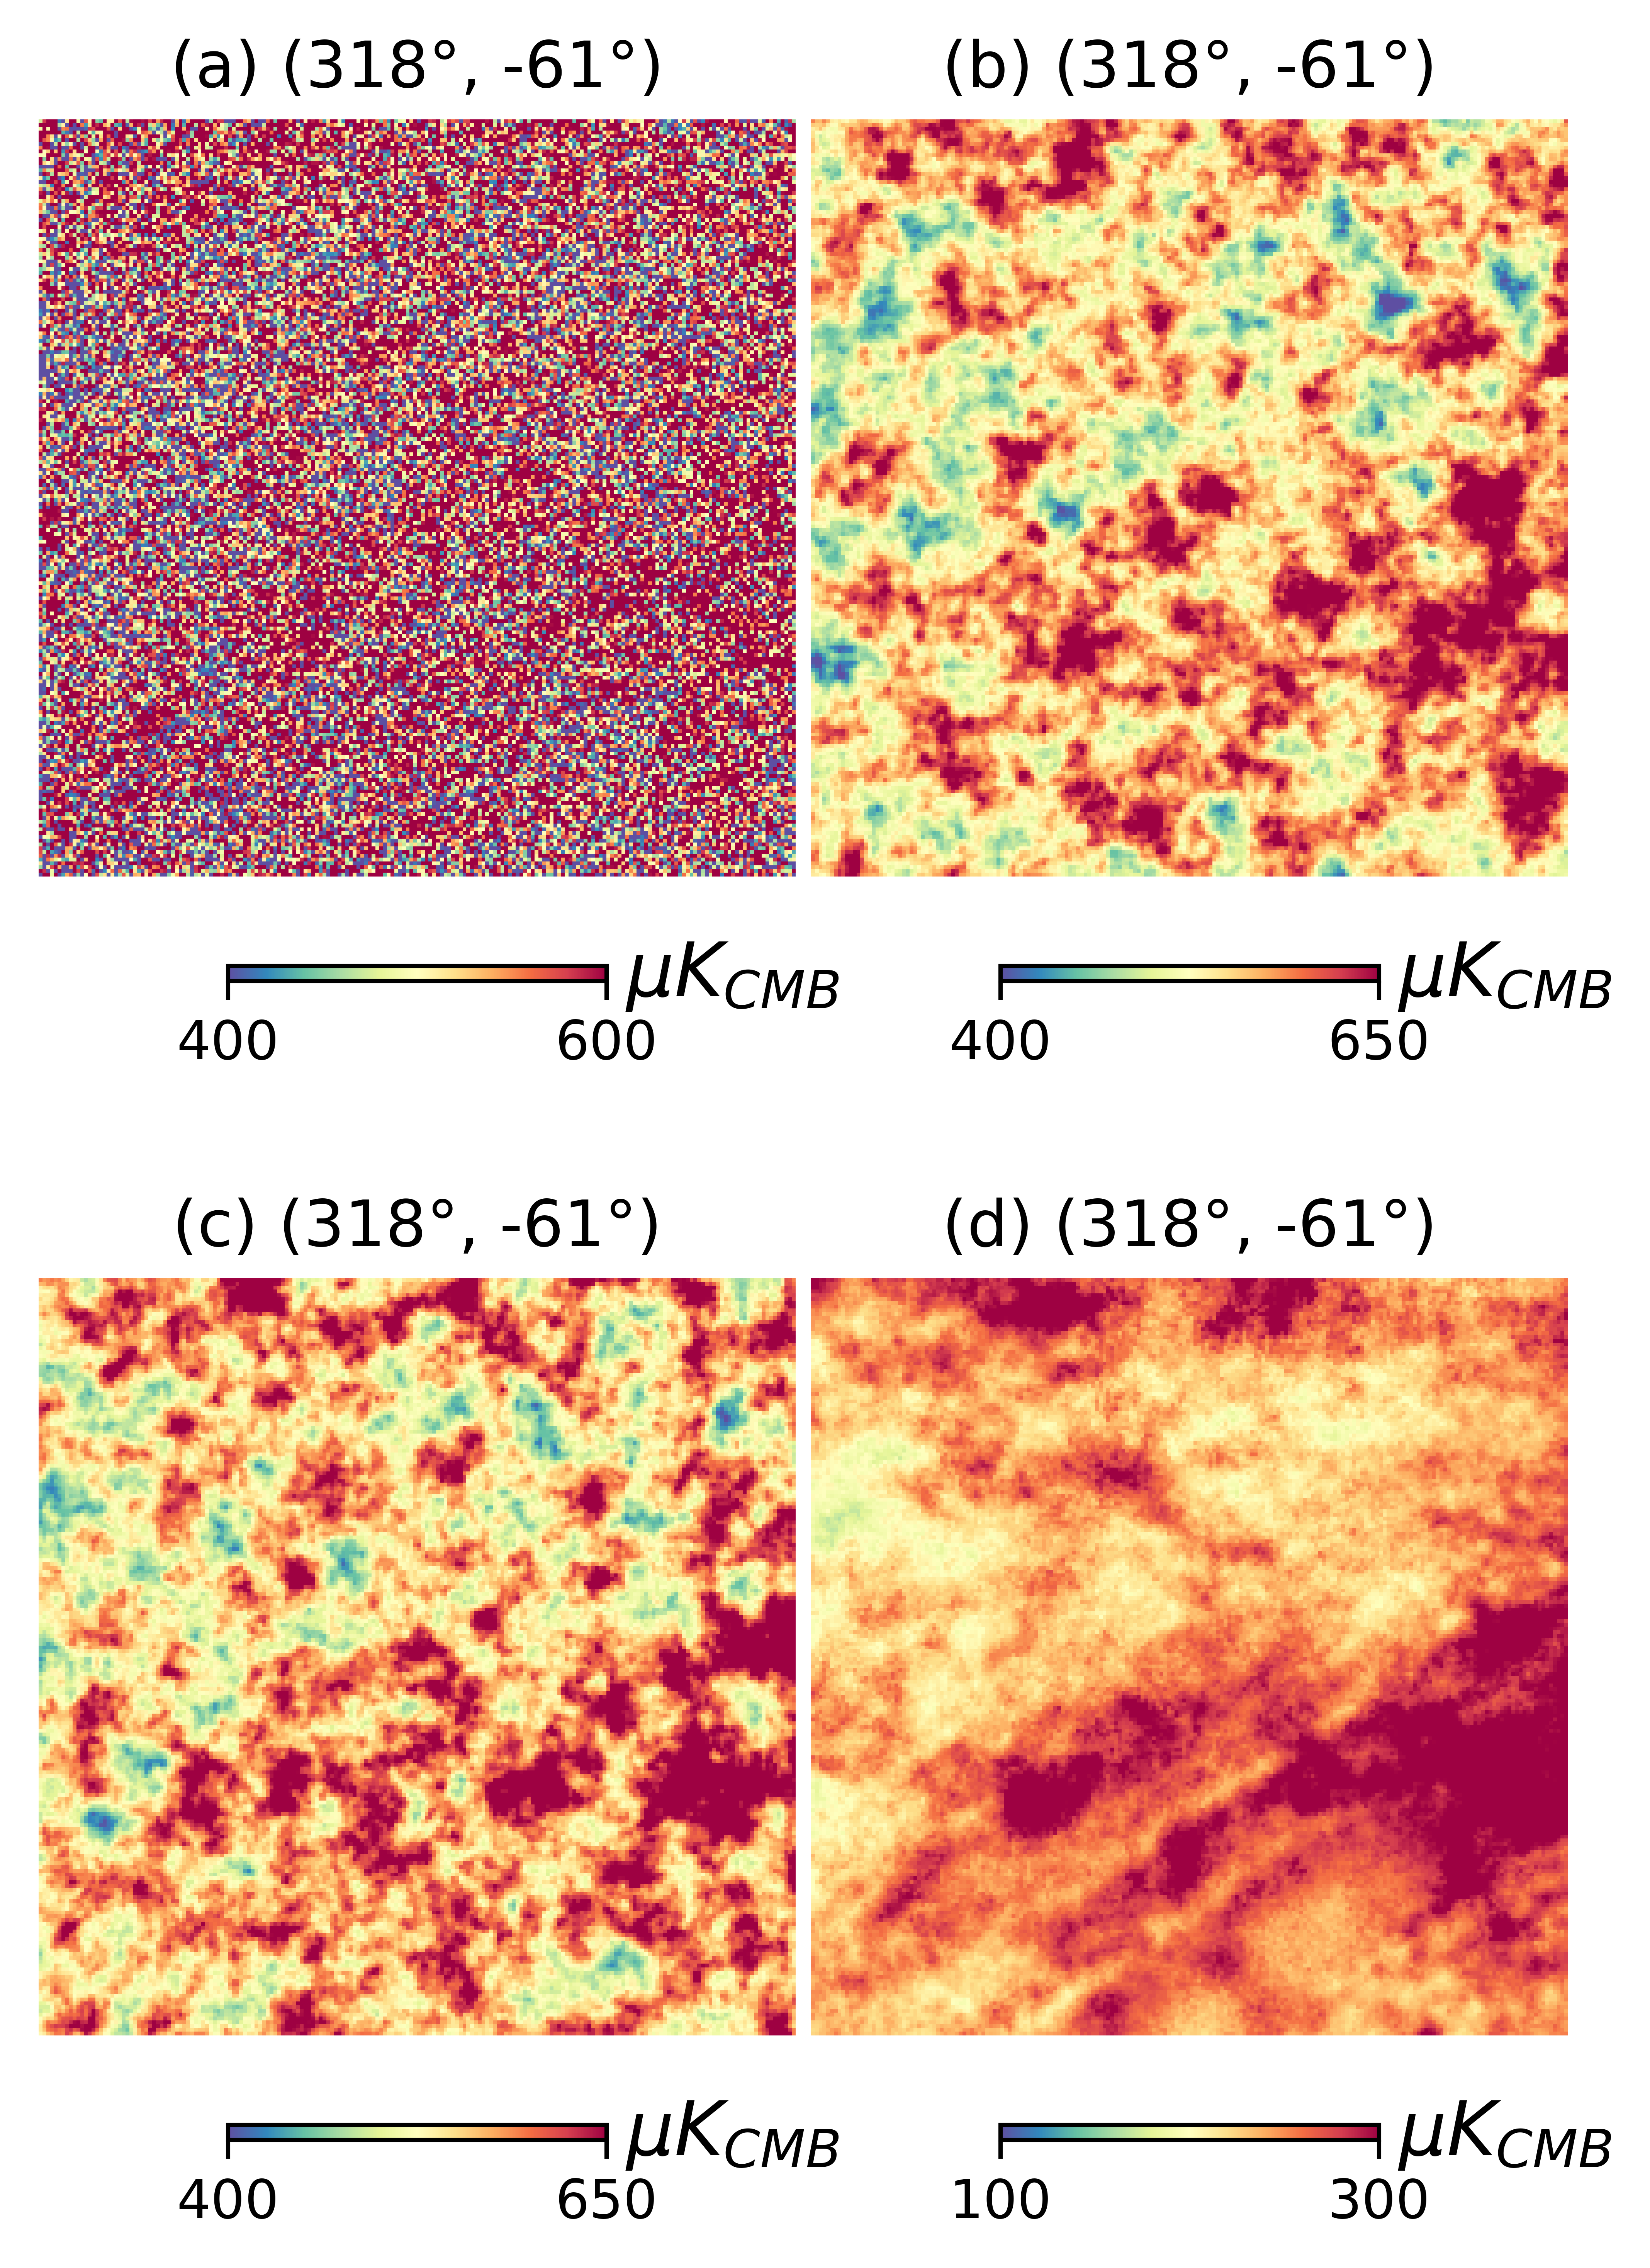
\includegraphics[width=0.48\textwidth]{figures/BK_non_smooth_wo_zero_lvl.png}
    \caption{Dust intensity at 353GHz at [l = 318, b = -61] with an angular resolution of $30\arcmin$: (a) PR3 (b) d9 (c) d11 (d) d12. Here, PR3 is contaminated by CIB and extragalactic sources.}
    \label{fig:353_int_BK}
\end{figure}

\begin{figure}[ht!]
    \centering
    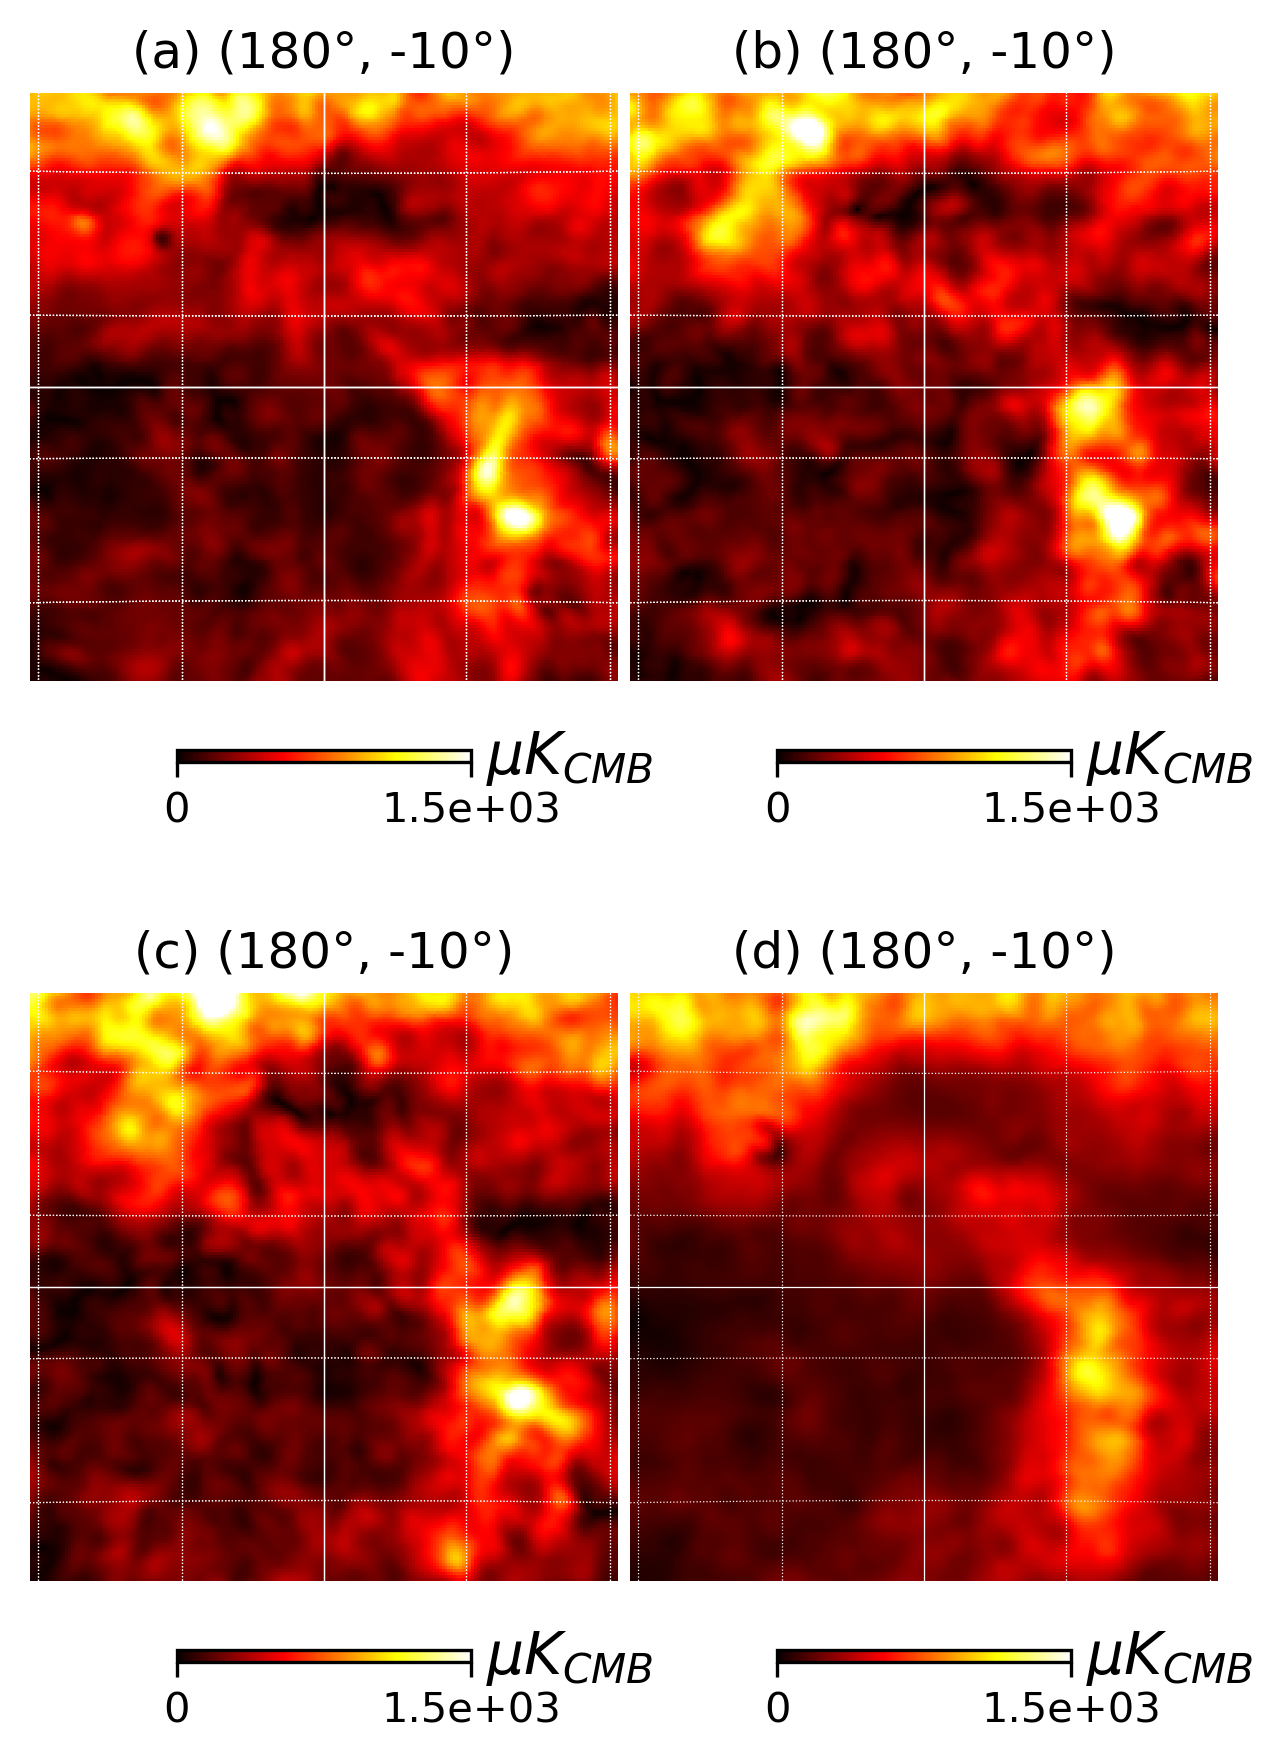
\includegraphics[width=0.48\textwidth]{figures/pol_gal_plane_smooth_30'.png}
    \caption{Polarized dust intensity at 353GHz centered at [l = 180, b = -10], smoothed to $30\arcmin$: (a) PR3 (b) d9 (c) d11 (d) d12.}
    \label{fig:353_pol_int_gal_plane}
\end{figure}
% \begin{figure}
%     \centering
%     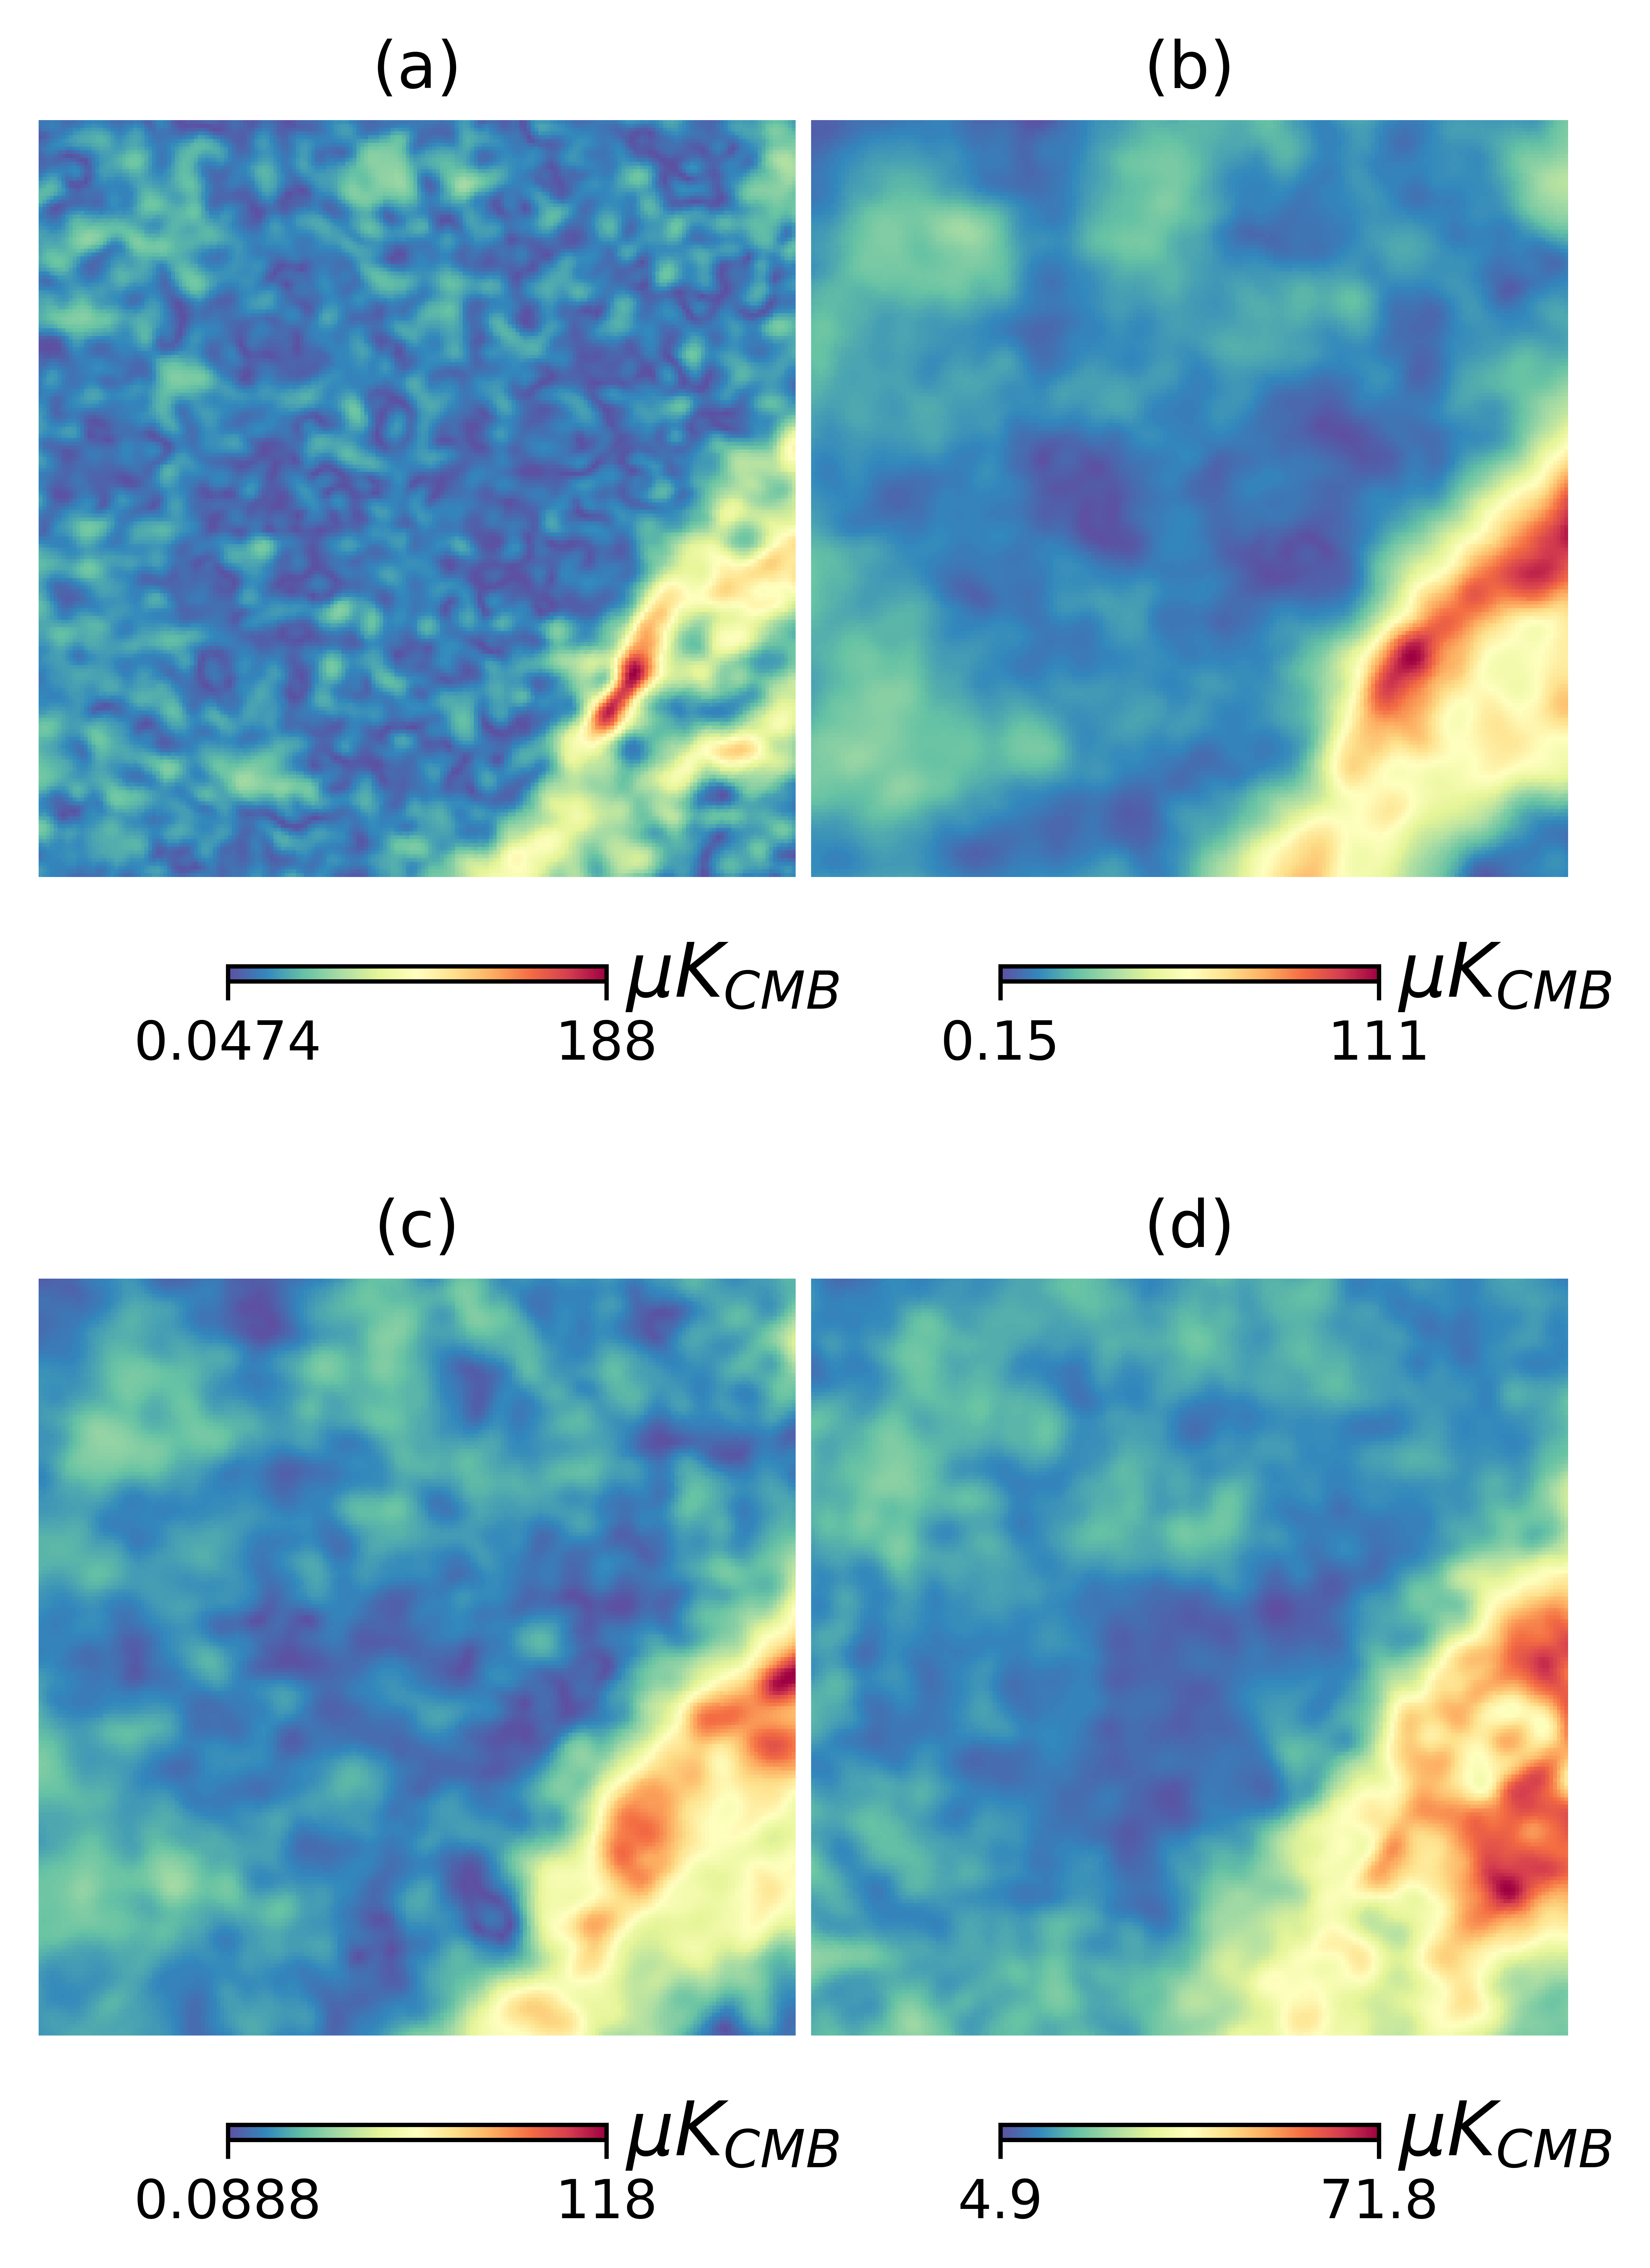
\includegraphics[scale = 0.6]{figures/pol_NGP_smooth_30'.png}
%     \caption{Polarized dust intensity at 353GHz centered at [l = 0, b = 90].}
%     \label{fig:353_pol_int_NGP}
% \end{figure}

\begin{figure}[ht!]
    \centering
    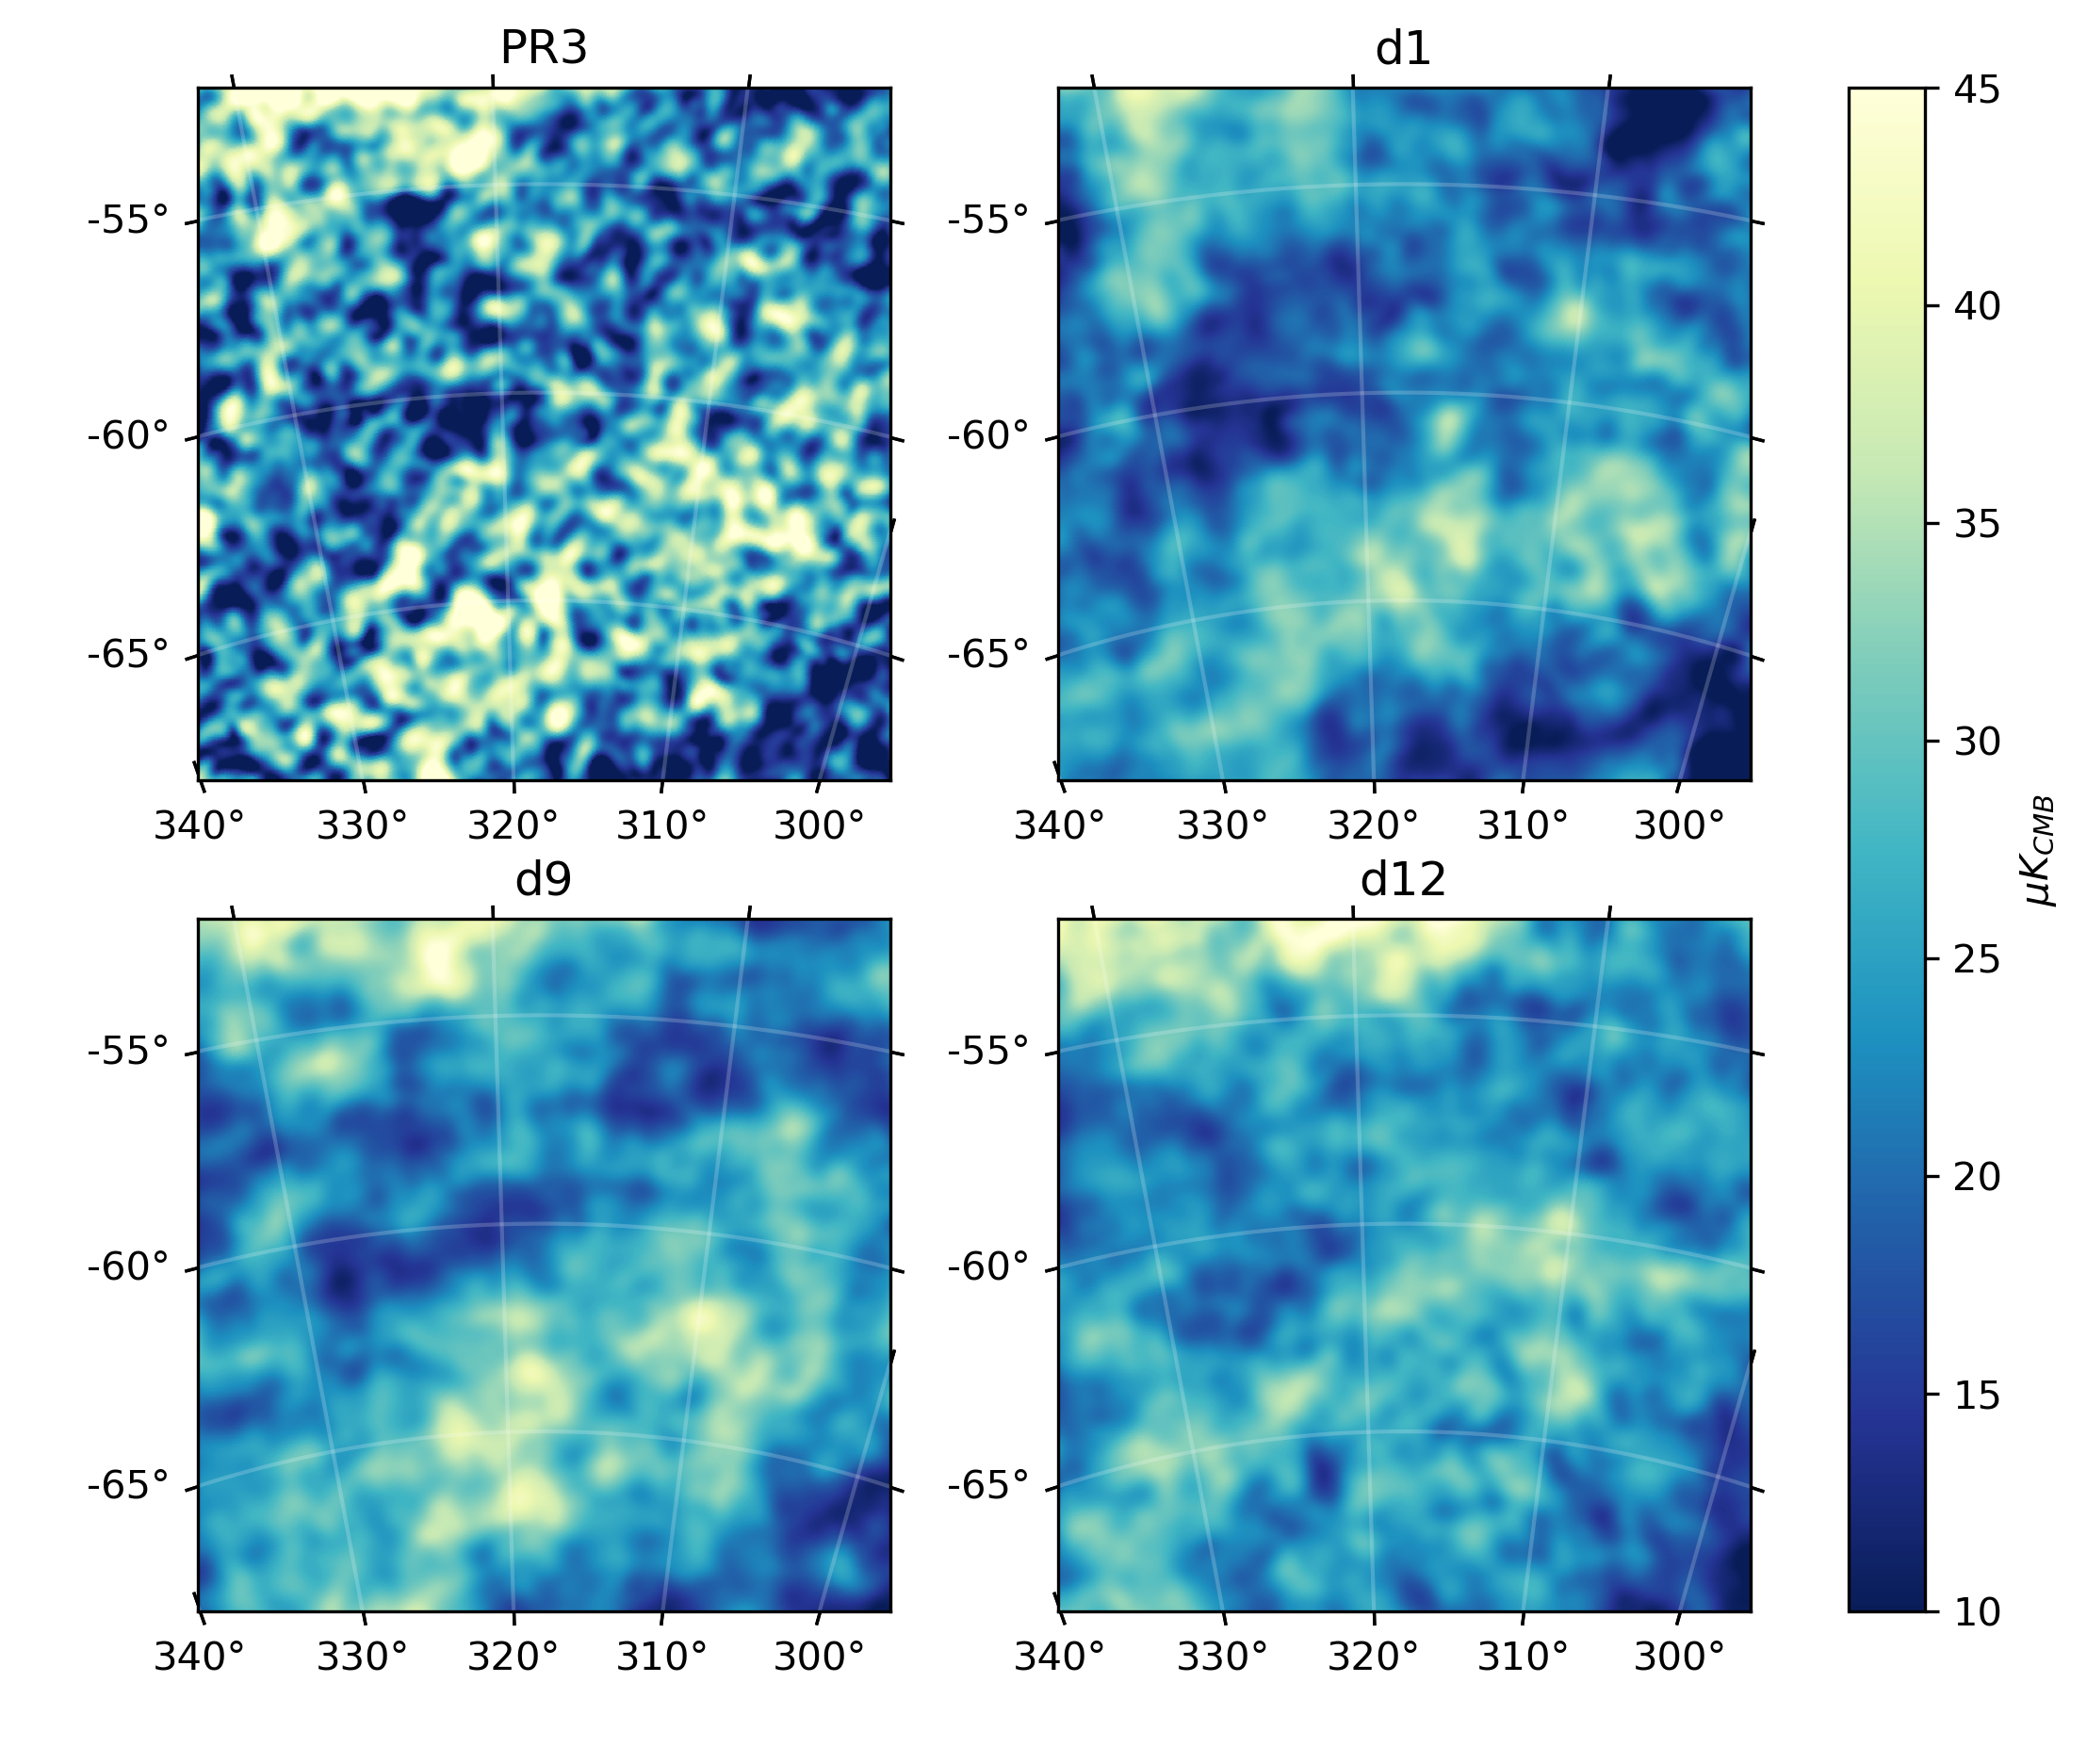
\includegraphics[width=0.48\textwidth]{figures/pol_BK_smooth_30'.png}
    \caption{Polarized dust intensity at 353GHz centered at [l = 318, b = -61], smoothed to $30\arcmin$: (a) PR3 (b) d9 (c) d11 (d) d12.}
    \label{fig:353_pol_int_BK}
\end{figure}

Intensity and polarization at 353~GHz are displayed in Figures~\ref{fig:353_int_gal_plane} to \ref{fig:353_pol_int_BK}. 
%Varying choices for filtering the real data and generation of random small scales result in varying dust emission properties. 
In total intensity, d9 and d11 are very similar (with small differences due to the fact that different seeds are used to generate small scale structures). Real structures are replaced by random realizations as described in section \ref{sec:small_scales}, while for intensity d12 is more similar to the actual data by construction at small scales, and more filamentary. 
% Around the BICEP/Keck patch center (Figure~\ref{fig:353_int_BK}), the PR3 data are contaminated by the CIB, which masks out dust emission. 

For the polarized intensity, close to the Galactic plane (Figure \ref{fig:353_pol_int_gal_plane}), we see a resemblance between the data and the three models. Near the Galactic poles, the signal is fainter, but there is a visual general agreement between the models and the data. 
%After smoothing with a Gaussian beam of 30 arcmin, we discern dust structures.
\subsection{Power spectra}
\label{sec:PS-validation}

\subsubsection{Dust Emission}

To compare the performance of the latest PySM dust models \texttt{d9}, \texttt{d10} and \texttt{d12} with real data over a broad range of scales, we present their power spectra computed on both large-area and small-area masks. We first apply the defined masks to the mean-subtracted PySM dust models and NPIPE ``A''/``B'' detector-split maps at delta 353~GHz. We then use \texttt{anafast} to compute the cross-spectra of the masked NPIPE data split maps to minimize noise correlation, bin the spectra with a dynamic $\ell$ interval optimized for map noise, and scale the results into the full-sky $\mathcal{D}_\ell$, accounting properly for the $f_{\mathrm{sky}}$ of the mask. The error bars associated to these cross-spectra are given by the method stated in \cite{Tristram:2005}. The same method is applied to calculate the auto-spectra of the masked model maps. 

%We define a set of Galactic masks starting from the unapodized Galactic masks\footnote{\texttt{HFI\_Mask\_GalPlane-apo0\_2048\_R2.00.fits} distributed \url{https://pla.esac.esa.int}} by the Planck collaboration via the Planck Legacy Archive. There are eight masks in total, leaving between 20\% and 99\% of the sky available for analysis. We apodize each mask with a cosine taper of characteristic length $2^\circ$ resulting in nine masks: \texttt{GAL015}, \texttt{GAL034}, \texttt{GAL052}, \texttt{GAL062}, \texttt{GAL072}, \texttt{GAL082}, \texttt{GAL092}, \texttt{GAL096}, where the number indicates the percentage of the sky left for analysis, i.e., $100 f_{\rm sky}$.  

For our large-area comparison, we use a set of $2^\circ$-apodized Galactic masks\footnote{\texttt{HFI\_Mask\_GalPlane-apo2\_2048\_R2.00.fits} distributed \url{https://pla.esac.esa.int}} by the Planck collaboration via the Planck Legacy Archive. There are eight masks in total, leaving between 20\% and 99\% of the sky available, in which we take four representative ones for our analysis. It results in masks \texttt{GAL020}, \texttt{GAL040}, \texttt{GAL060} and \texttt{GAL080}, where the number indicates the percentage of the sky left for analysis, i.e., $100 f_{\rm sky}$. In Figure~\ref{fig:largefield_power} we show the $TT$, $EE$, and $BB$ power spectra of the \dnine{} model, and of the GNILC maps from which the \dnine{} model was derived, computed on four of the Galactic masks described above. ... 

%We present power spectra computed on large-area Galactic masks. We define a set of Galactic masks starting from the unapodized Galactic masks\footnote{\texttt{HFI\_Mask\_GalPlane-apo0\_2048\_R2.00.fits} distributed \url{https://pla.esac.esa.int}} by the Planck collaboration via the Planck Legacy Archive. There are eight masks in total, leaving between 20\% and 99\% of the sky available for analysis. We apodize each mask with a cosine taper of characteristic length $2^\circ$ resulting in nine masks: \texttt{GAL015}, \texttt{GAL034}, \texttt{GAL052}, \texttt{GAL062}, \texttt{GAL072}, \texttt{GAL082}, \texttt{GAL092}, \texttt{GAL096}, where the number indicates the percentage of the sky left for analysis, i.e., $100 f_{\rm sky}$.  

%In Figure~\ref{fig:spectra_by_field} we show the $TT$, $EE$, and $BB$ power spectra of the \dnine{} model, and of the GNILC maps from which the \dnine{} model was derived, computed on four of the Galactic masks described above.

\begin{figure}
    \centering
    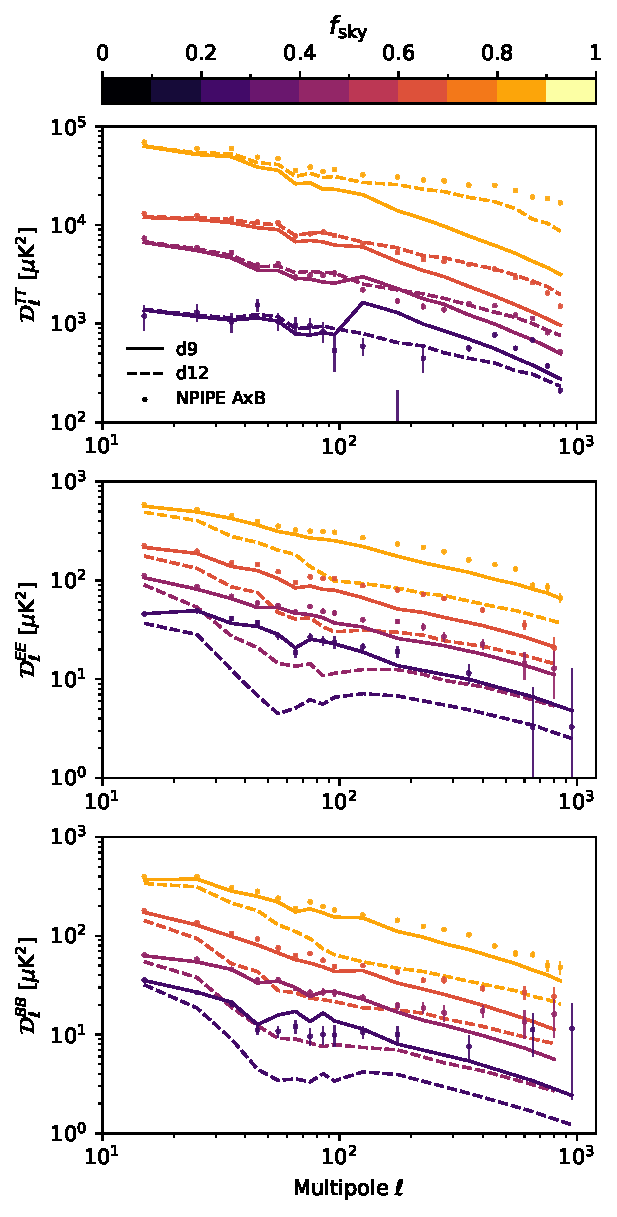
\includegraphics[width=\columnwidth]{figures/largefield_power_all_TEB_pub.pdf}
    \caption{$TT$, $EE$ and $BB$ power spectra of the \texttt{d9} model (solid lines), the \texttt{d12} model (dashed lines) and the NPIPE detector-split maps (circle scatters) when computed on the \texttt{GAL020}, \texttt{GAL040}, \texttt{GAL060} and \texttt{GAL080} Galactic masks. Each set of comparisons is colored in the same color representing their sky fraction $f_{\mathrm{sky}}$. Note that we do not show the \texttt{d10} results as this model is identical to \texttt{d9} at 353~GHz.}
    \label{fig:largefield_power}
\end{figure}

%\begin{figure*}
%    \centering
%    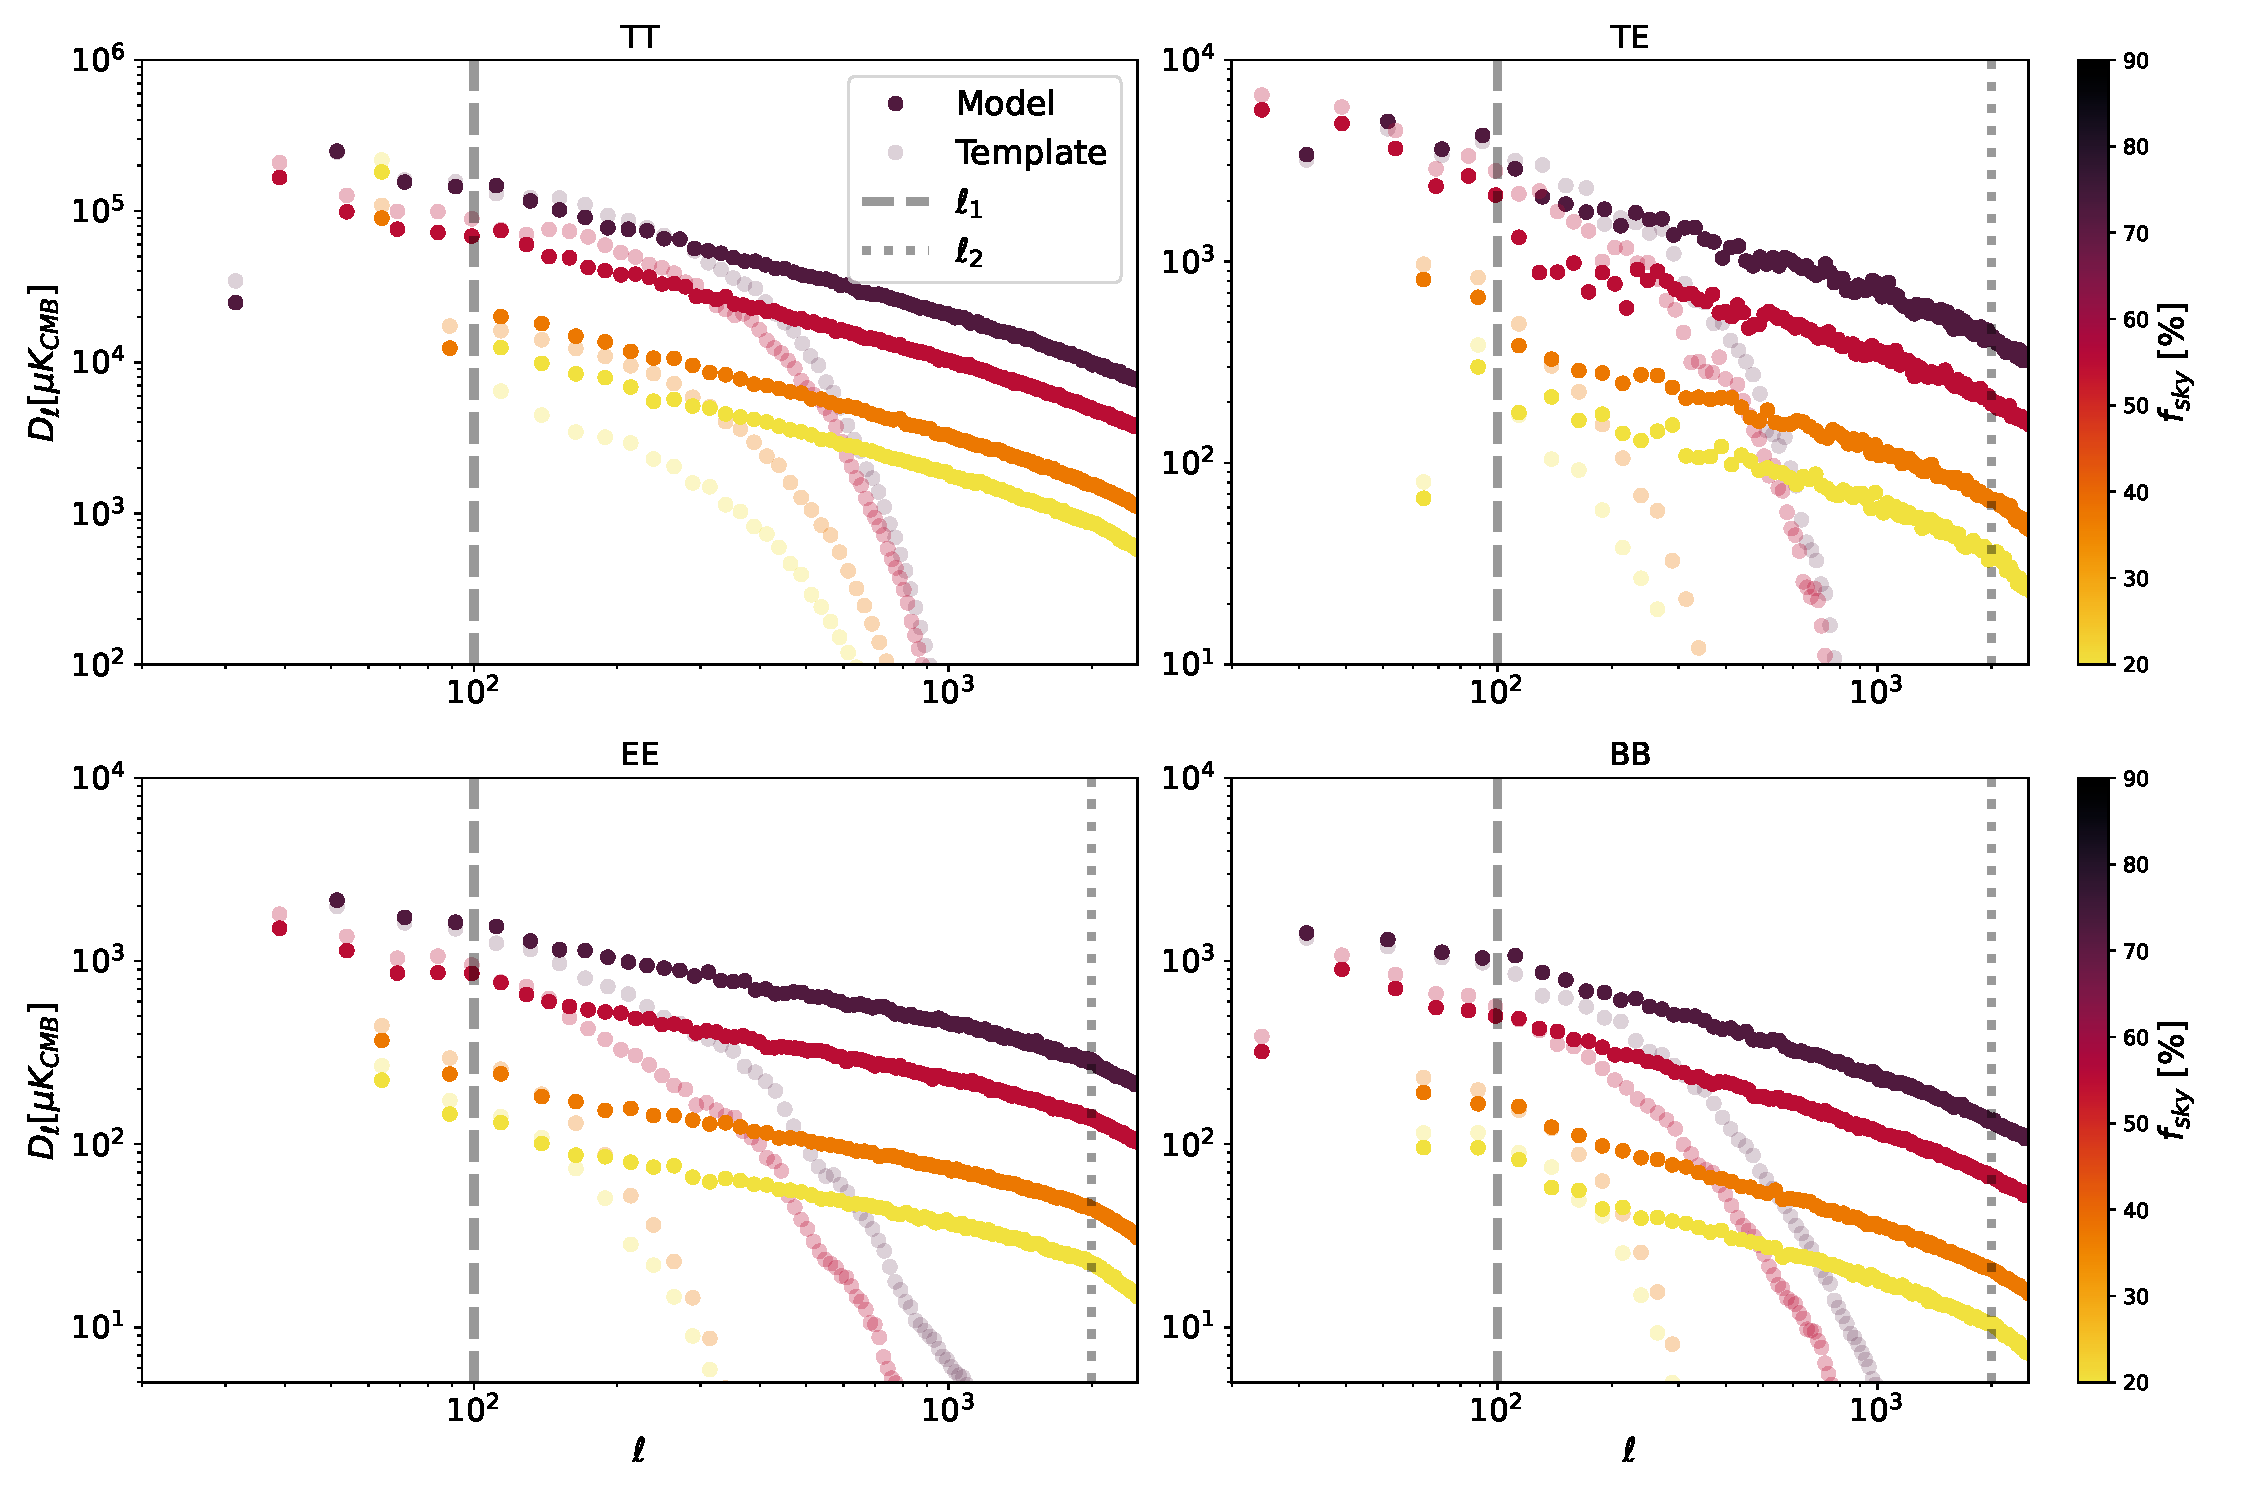
\includegraphics[width=2.\columnwidth]{figures/dust_valspectra.pdf}
%    \caption{This figure compares the power spectra of the \dnine{} model (dark circles) and the input GNILC map (light circles) when computed on the \texttt{GAL090}, \texttt{GAL070}, \texttt{GAL040}, and \texttt{GAL020} Galactic masks.}
%    \label{fig:spectra_by_field}
%\end{figure*}

\begin{figure}
    \centering
    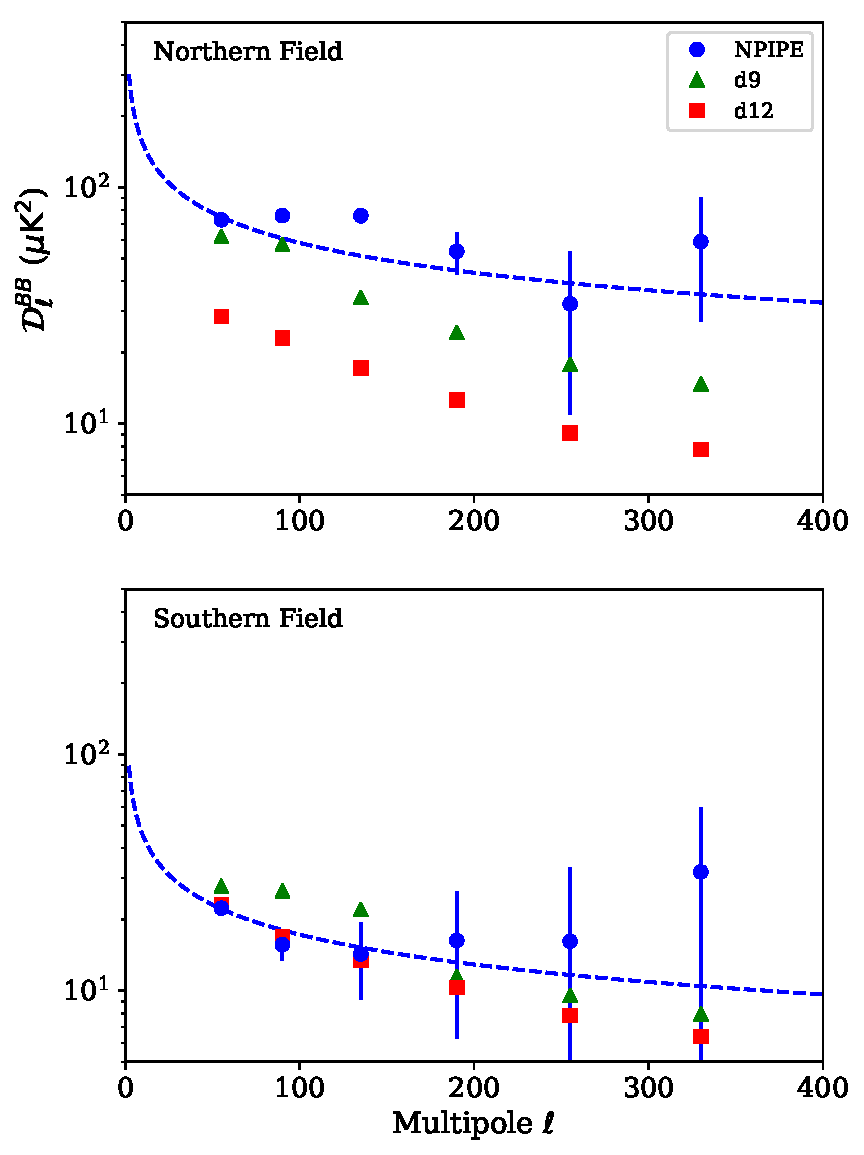
\includegraphics[width=0.48\textwidth]{figures/smallfield_power.pdf}
    \caption{The binned $BB$ power spectra from the 353~GHz NPIPE half-ring split maps and dust model maps \texttt{d9} and \texttt{d12}. The model maps are integrated with a 353~GHz delta bandpass and the NPIPE data maps are color-corrected (i.e. scaled by a factor of 0.92) to the same single frequency. The dashed lines indicate the best-fit of the fixed-index power law ($\mathcal{D}_\ell^{BB} = A^{BB} \big( l/80 \big)^{\alpha^{BB}+2}$ where $\alpha^{BB} = -2.42$) to the NPIPE data points, which is largely driven by the first two band powers.}
    \label{fig:smallfield_power}
\end{figure}

In our small-area case, we mainly follow the analysis method described in \cite{planck2014-XXX} to define the masks for spectra computation. We first use a HEALPix grid with $\texttt{nside} = 8$ to divide the full sky into 768 patches. At the center of each patch, we create a 400-square-degree circular mask with its edge tapered by a $2^\circ$ FWHM Gaussian, resulting in $f_{\rm sky} \approx 0.008$. We then compute the $BB$ auto-spectra of the masked model maps at bin centers $\ell = 55,90,135,190,255,330$ with a dynamic top-hat binning $\Delta \ell = 30,40,50,60,70,80$, and scale them to be the full-sky $\mathcal{D}_\ell^{BB}$. The representative results from two selected circular fields at $|b| > 30^\circ$ of the northern and southern Galactic hemispheres are shown in Fig.~\ref{fig:smallfield_power}. 

%To compare the small-scale performances of the latest PySM dust models \texttt{d9}, \texttt{d10} and \texttt{d12} with real data, we mainly follow the analysis method described in \cite{planck2014-XXX} to examine the model behaviors. We first use a HEALPix grid with $\texttt{nside} = 8$ to divide the full sky into 768 patches. At the center of each patch, we create a 400-square-degree circular mask with its edge tapered by a $2^\circ$ FWHM Gaussian (resulting in $f_{\rm sky} \approx 0.008$), and apply such a mask to the mean-subtracted dust model and NPIPE half-ring split maps at 353~GHz. We then use \texttt{anafast} to compute the $BB$ auto-spectra of the masked model maps at bin centers $\ell = 55,90,135,190,255,330$ with a dynamic top-hat binning $\Delta \ell = 30,40,50,60,70,80$, and scale them to be the full-sky $\mathcal{D}_\ell^{BB}$, accounting properly for the $f_{\mathrm{sky}}$ of the circular mask. For the masked NPIPE data maps, we instead compute cross-spectrum from the two split maps to minimize the noise correlation. The representative results from two selected circular fields at $|b| > 30^\circ$ of the northern and southern Galactic hemispheres are shown in Fig.~\ref{fig:smallfield_power}. 

As one of the major science missions of CMB experiments is to acquire high precision primordial B-mode polarization measurements from a small sky patch, we would like to explore whether the PySM models can reproduce the dust $BB$ power spectrum's amplitude and steepness over $\ell$ in reality, especially in those high Galactic latitude small fields which could be part of future observation fields. We therefore compute the low-$\ell$ averaged $\mathcal{D}_\ell^{BB}$ (over $\ell = 55, 90$) and the high-$\ell$ averaged $\mathcal{D}_\ell^{BB}$ (over $\ell = 135, 190, 255, 330$) of each small field for the model and NPIPE maps, and we present the results in scatter plots in Fig.~\ref{fig:smallfield_power_all}. It turns out that the amplitude of the \texttt{d12} model is in general smaller than the preference of NPIPE data, as a large fraction of the d12 data points cluster around the lower-left corner of the plot. The wider span of the \texttt{d12} data points along the vertical direction also implies the model spectrum steepness varies more over the sky. In contrast, the \texttt{d9}/\texttt{d10} data points are fairly compatible with the NPIPE results, although they predict slightly steeper power spectra. If we define the ratio of the low-$\ell$ mean value to the high-$\ell$ mean value as a proxy for describing the spatial power change across the modulation scale, while the perfect fixed-index power law $\mathcal{D}_\ell^{BB} \propto \ell^{-0.42}$ yields a value of $\approx 1.60$, the NPIPE maps give $1.86 \pm 0.93$ and the \texttt{d9}/\texttt{d10} (\texttt{d12}) model map gives $2.37 \pm 0.77$ ($2.24 \pm 0.87$) over sky patches with $|b| > 30^\circ$.

\begin{figure}
    \centering
    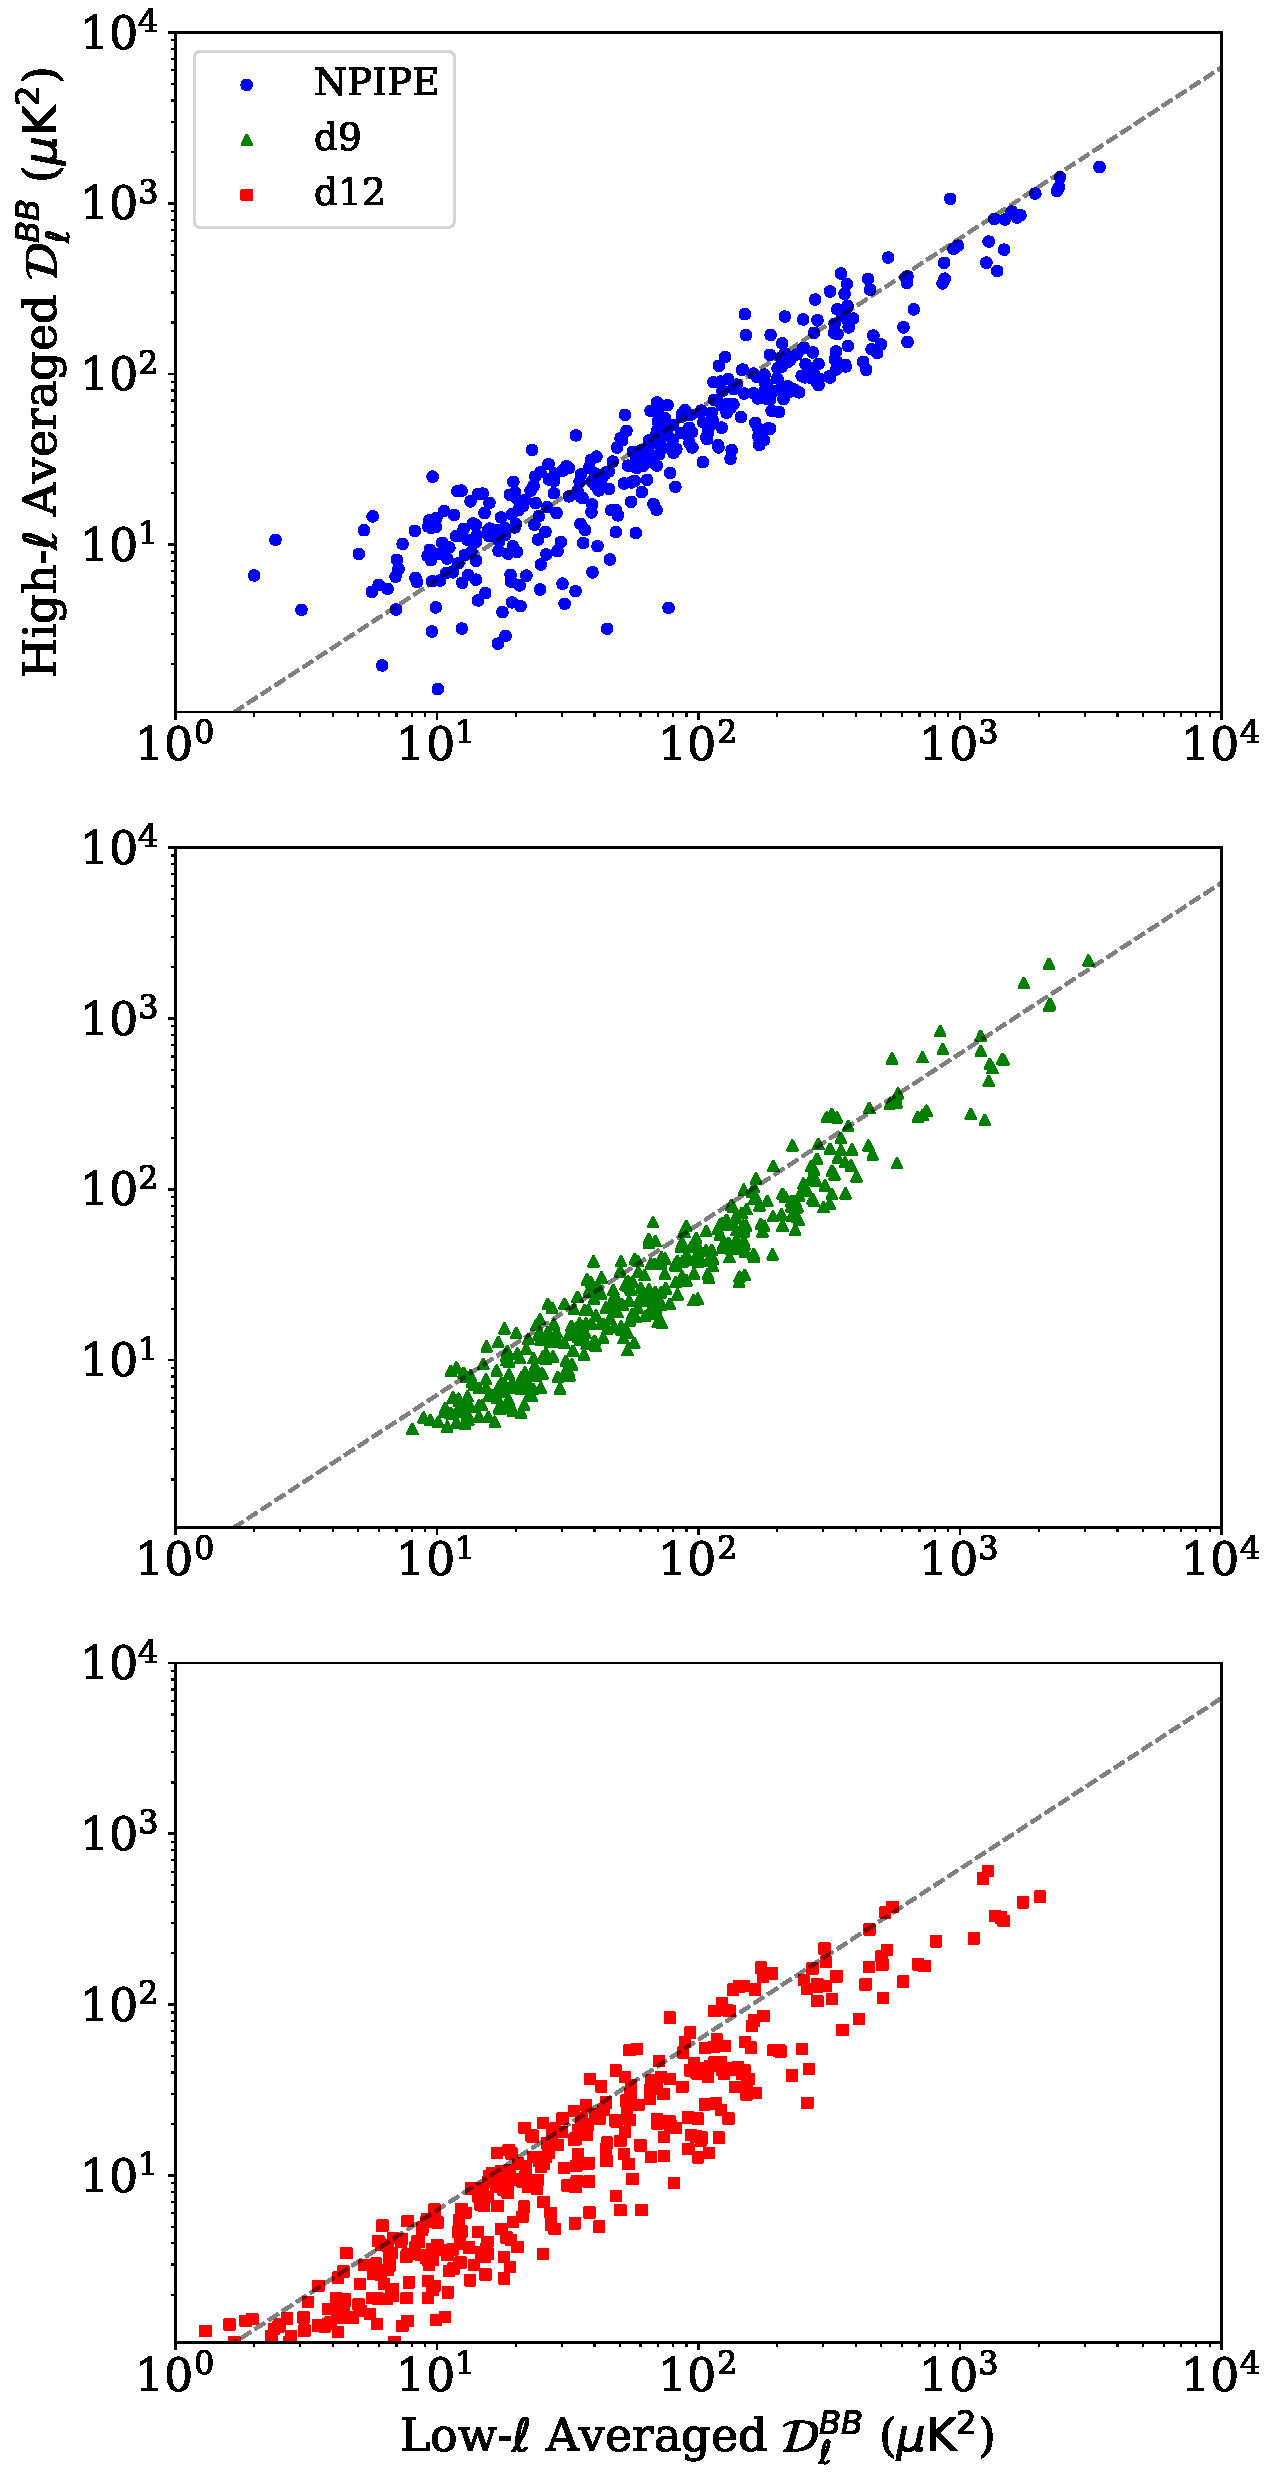
\includegraphics[width=0.48\textwidth]{figures/all2_lhmean.pdf}
    \caption{Scatter plots of the mean of the first two $BB$ band powers versus the mean of the last four $BB$ band powers shown in Fig.~\ref{fig:smallfield_power}. Each data point represents the results from a circular sky patches with $|b| > 30^\circ$. Dashed reference lines indicating $\mathcal{D}_\ell^{BB} \propto \ell^{-0.42}$ are added to the plots. This power law in fact comes from the analysis of several larger sky regions ($f_\text{sky} = 0.3 \; \text{to} \; 0.8$) by \cite{planck2014-XXX}, but the small-field NPIPE data points, which spread out when the dust amplitude is small presumably due to map noise, are consistent with it as well. Another important feature is that the trends of the \texttt{d9} and \texttt{d12} data points are lower than that of the NPIPE in these log-log plots, implying that the model spectra are steeper.}
    \label{fig:smallfield_power_all}
\end{figure}

\subsubsection{Synchrotron Emission}

\begin{figure*}
    \centering
    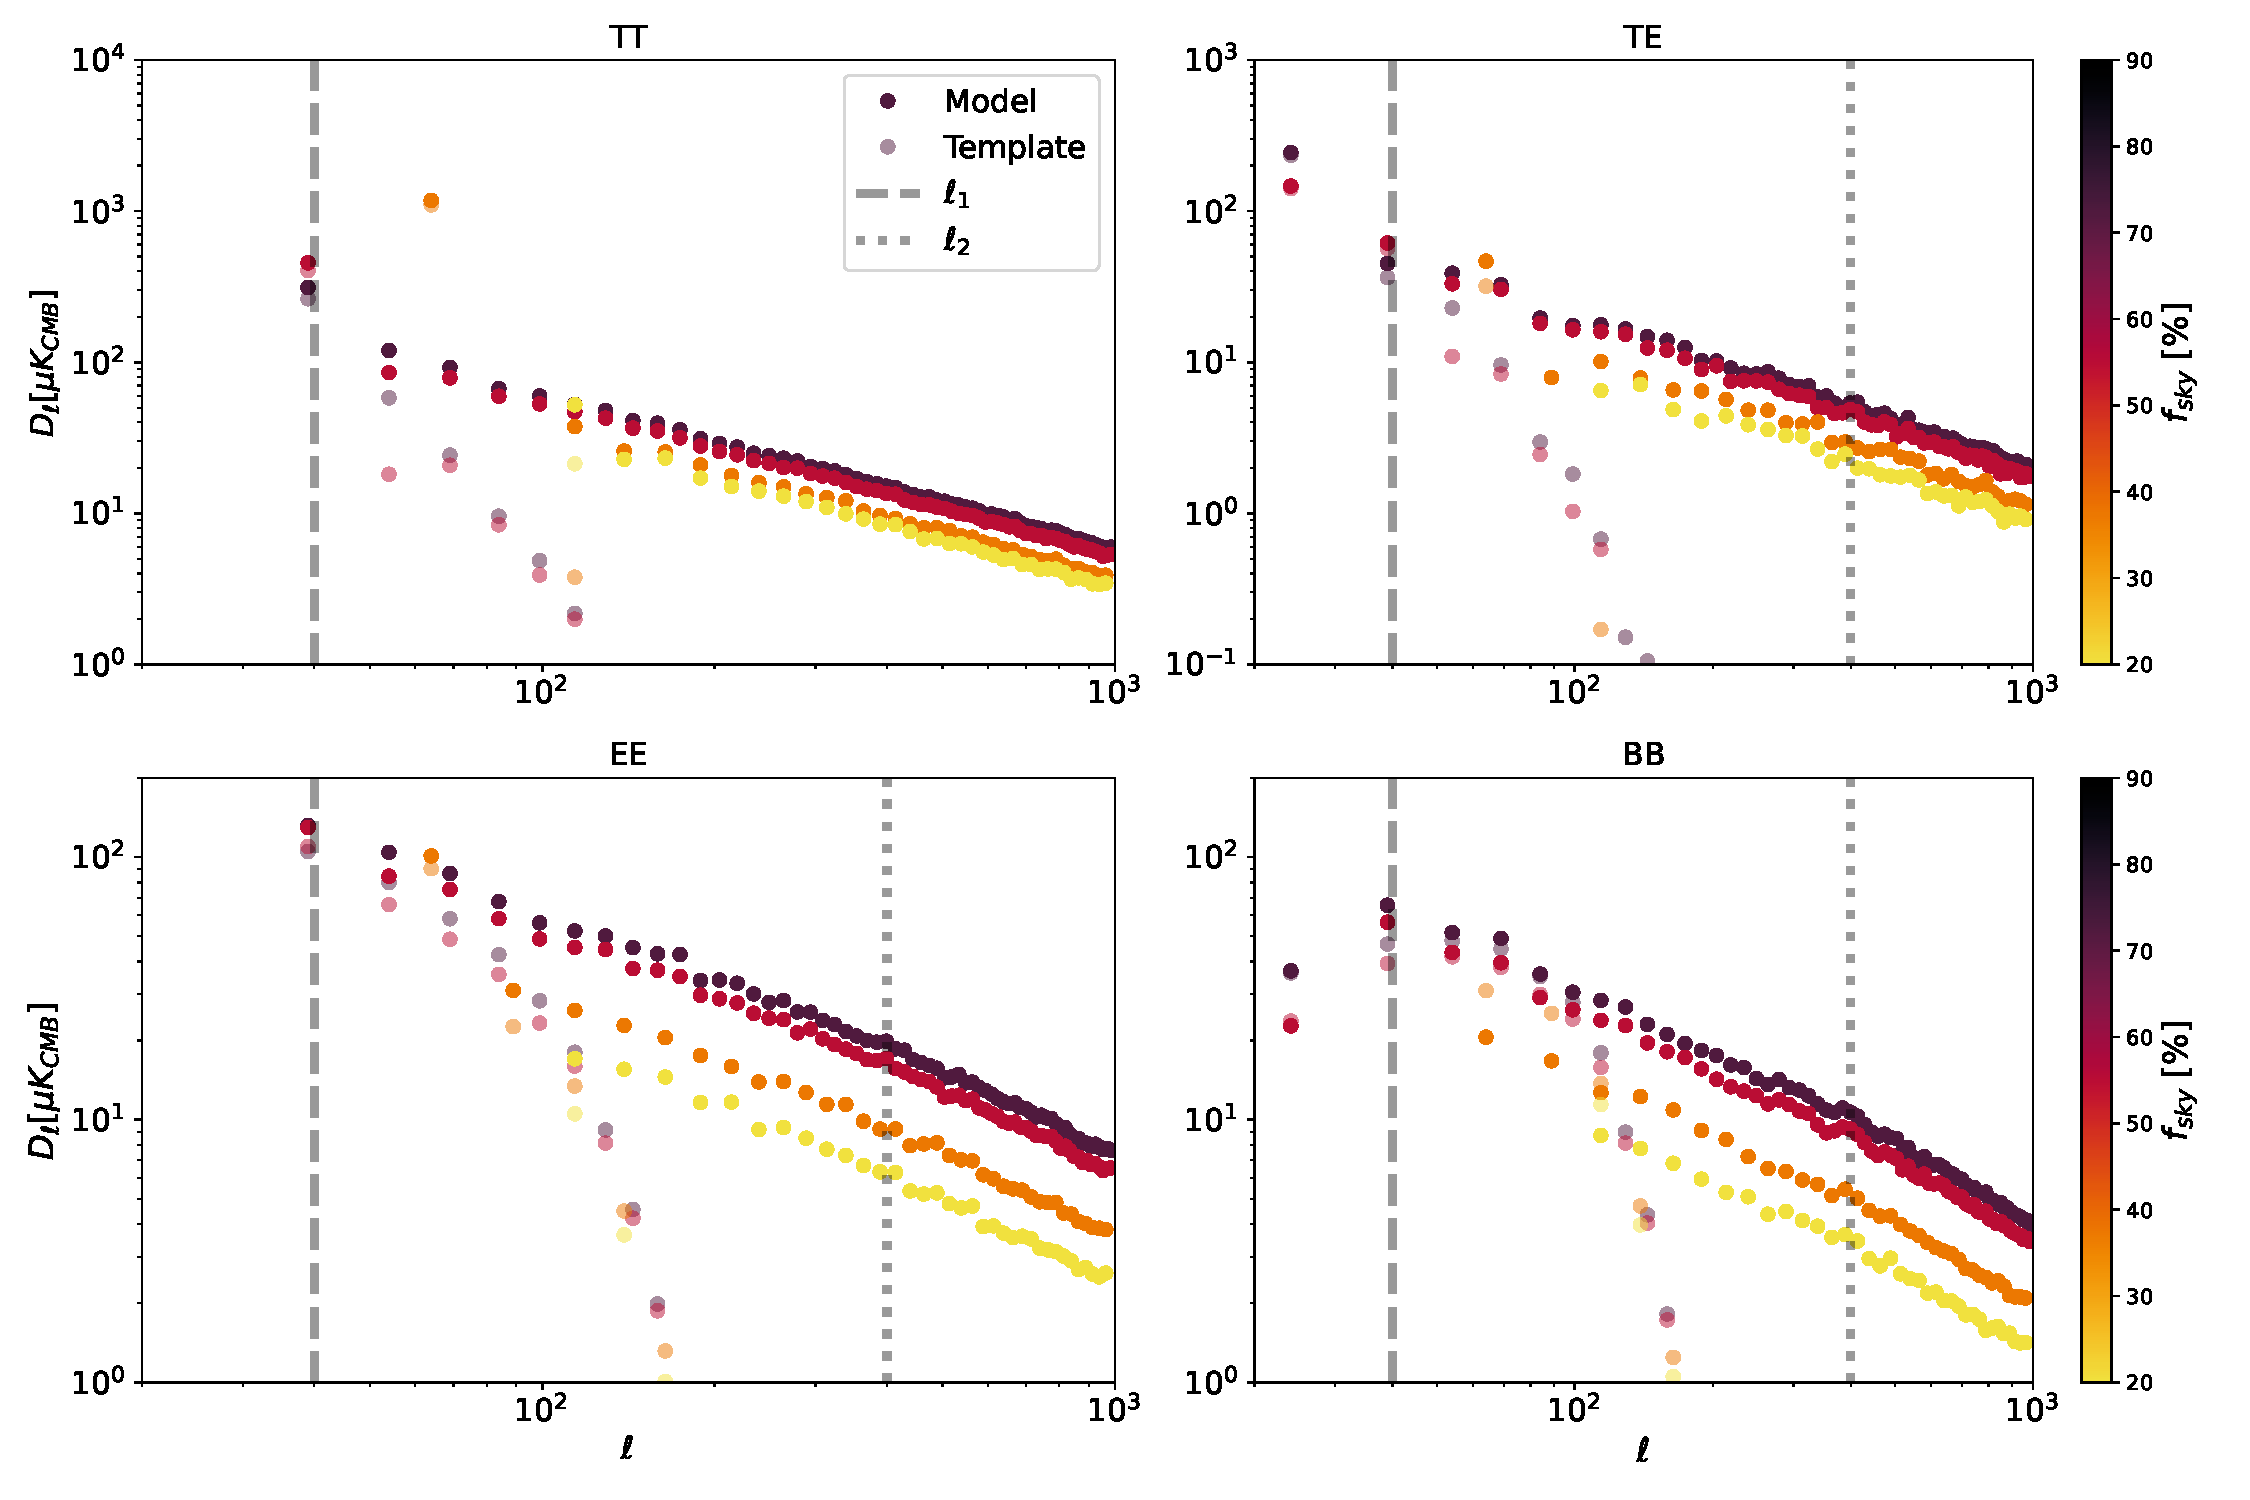
\includegraphics[width=2.\columnwidth]{figures/synch_valspectra.pdf}
    \caption{This figure compares the power spectra of the \texttt{s4} model (dark circles) and the input HASLAM/WMAP K-band  map (light circles) when computed on the \texttt{GAL090}, \texttt{GAL070}, \texttt{GAL040}, and \texttt{GAL020} Galactic masks.}
    \label{fig:spectra_by_field}
\end{figure*}
In this section we detail the validation of the new synchrotron models by comparing the power spectra with observations. For validating the PySM synchrotron temperature models, we use the synchrotron map from the BeyondPlanck re-analysis of Planck LFI data \citep{BeyondPlanck23}. BeyondPlanck released a synchrotron map\footnote{\url{https://beyondplanck.science/products/files\_v1}} at a reference frequency of 30\,GHz and at $2^\circ$ angular resolution. We produce single frequency temperature maps for the different synchrotron models at 30\,GHz and smoothed with a Gaussian beam with FWHM = $2^\circ$.

We have purposefully chosen an earlier release of BeyondPlanck for our analysis. Later versions of BeyondPlanck, or its successor, CosmoGlobe produce synchrotron intensity maps at 408 MHz. The PySM synchrotron models s5 and s7 are not suitable for producing synchrotron simulations at 408 MHz. This is a consequence of scaling the Haslam map from 408 GHz to 30 GHz for constructing the template for synchrotron intensity. When this template is rescaled to 408 MHz, with scaling that varies over the the sky, the model fails. We do not recommend use of the s5 and s7 models below 10 GHz. Therefore, we validate our models with the synchrotron intensity map at 30 GHz.

% \giuse{In case of the synchrotron polarization, we  compare the models with band integrated observations. So, we compute bandpass integrated maps  with PySM~3 routines and for  the different synchrotron models. For the sake of fair comparison with Planck data, we adopt the average LFI 30\,GHz RIMO transmission \citep{planck2014-a03}.} The bandpass integrated maps are further smoothed with Gaussian beams of 33.1\arcmin beams to produce model maps at native resolutions of the LFI 30\,GHz data. Finally, the observed power spectra are computed by taking the cross-spectrum between independent detector splits, e.g. A and B, of the NPIPE \footnote{Publicly available through NERSC at \\ /global/cfs/cdirs/cmb/data/planck2020} (PR4) 30\,GHz maps \citep{planck2020-LVII}. 

For synchrotron polarization validation, we compare the models with Planck Revisited synchrotron polarization maps\footnote{\url{https://portal.nersc.gov/project/cmb/Planck\_Revisited}} \citep{Delabrouille2024}. These are the cleanest full sky maps of polarized synchrotron at 30 GHz, at $1^\circ$ resolution, at the time of analysis. We convert the Planck Revisited synchrotron maps from $\mu {\rm K_{RJ}}$ to $\mu {\rm K_{CMB}}$. 

The synchrotron power spectra is computed for four sky fractions, 80\%, 60\%, 40\% and 20 \%, like for the dust validation. However, we do not use the Planck Galactic masks for this. The Planck Galactic masks capture the shape of the Galactic dust signal, as it is the brightest foreground at CMB frequencies. The shape of the Galactic synchrotron signal differs significantly from the shape of the Galactic masks. Therefore, we construct masks for the synchrotron by thresholding the synchrotron polarized intensity smoothed with a $8.5^\circ$ beam. We additionally mask out a portion of the Galactic plane with a narrow band mask. This ensures that we are always excluding the Galactic plane. In Figure~\ref{fig:sync_masks} we show the regions of these masks. 

We also use the Planck Revisited point source mask to mask out the brightest point sources for the polarization analysis. The combined mask is apodized with a $2^\circ$-$6^\circ$ cosine taper. The apodization length increasing with decreasing sky fraction. The power spectrum is estimated with HEALPix \texttt{anafast} in the same way as for the dust. For the $EE$ and $BB$ spectra, we compute the noise bias and standard deviation from 200 noise realizations. The polarization power spectra are corrected for the noise bias. 

% \giuse{We estimated the synchrotron power spectra considering three choices of masks:  full sky  (100\%), 70\% and 50\% sky fractions. To produce the synchrotron  masks, we use the LFI 30\,GHz map of polarized intensity, smoothed with a Gaussian beam of $2^\circ$ FWHM, and masking all the pixels larger than  17 and 10 $\mu{\rm K}_{\rm CMB}$, as shown in Figure \ref{fig:sync_masks}.  Masks are tapered  with a $2^\circ$ cosine apodization.  For the polarization analysis, polarized point sources are also masked using the Planck-LFI DR2 mask\footnote{\bf @shamik could you add the filename reference?}. }
\begin{figure}
    \centering
    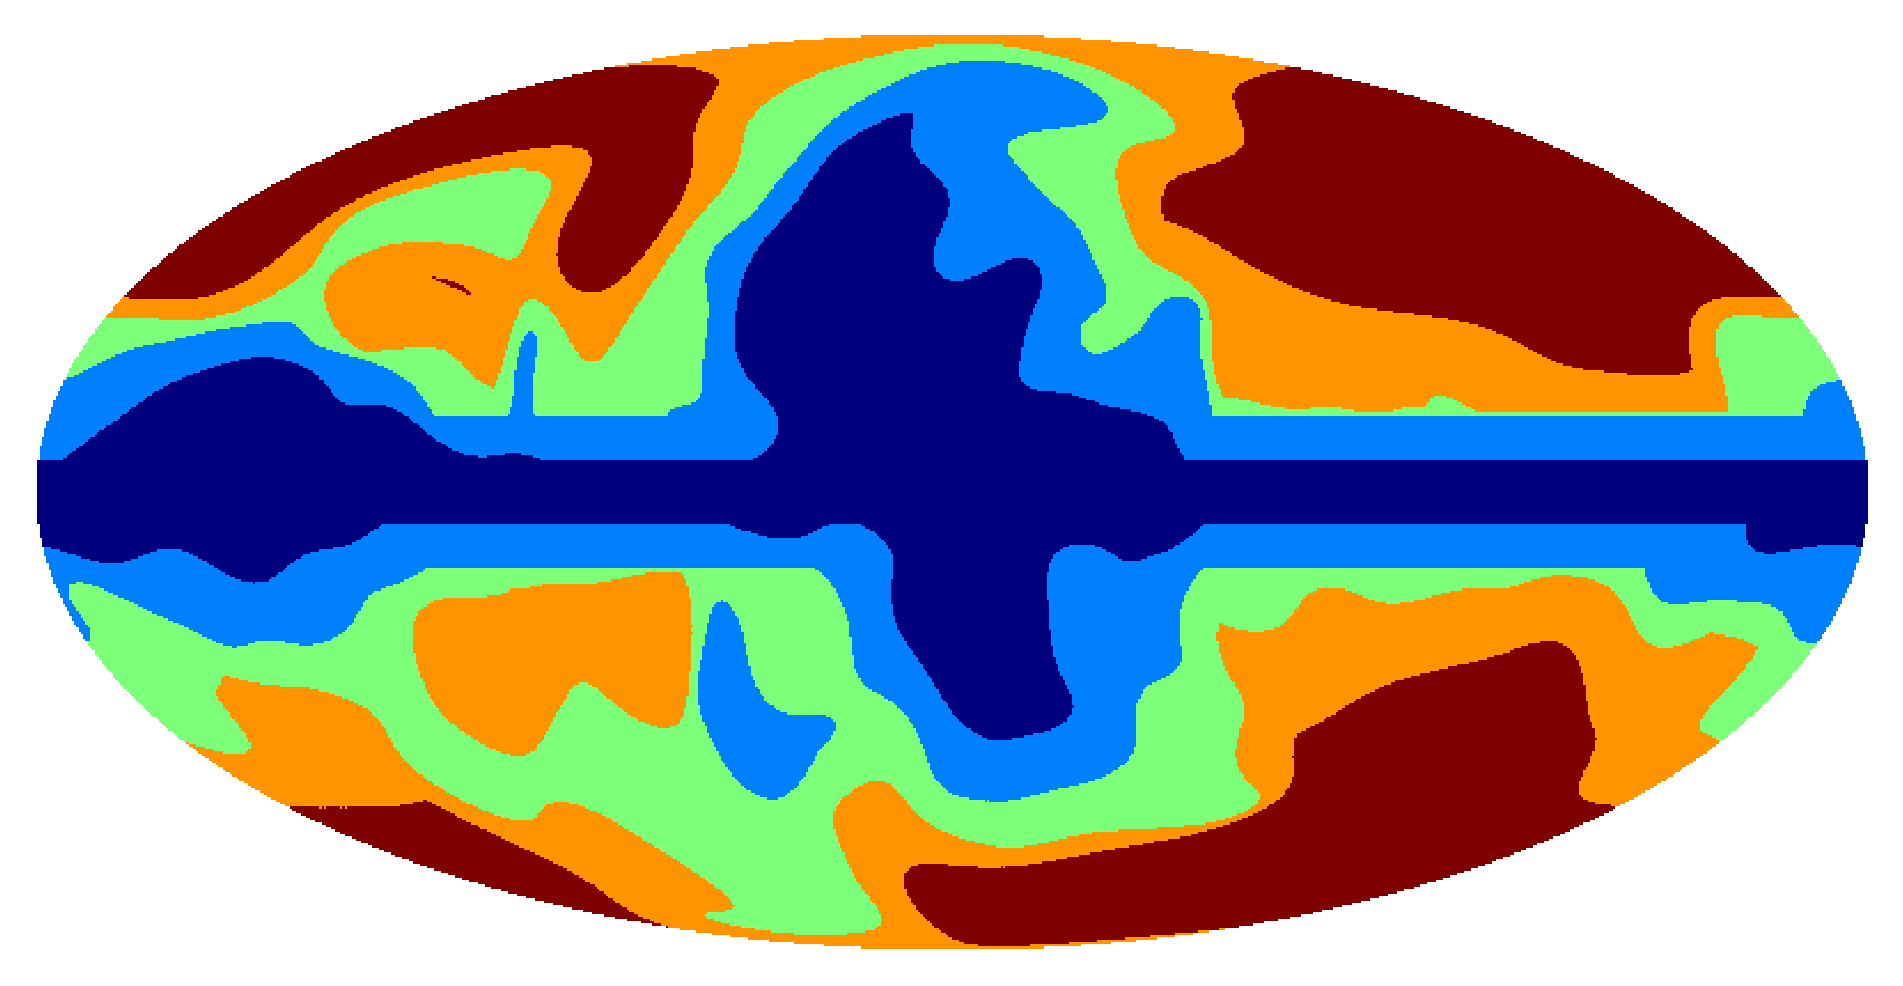
\includegraphics[width=0.46\textwidth]{figures/SYNC_mask_stack.png}
    \caption{Figure showing the four different Galactic masks used for the synchrotron validation. The red region is the 20 \% mask; the orange region shows the additional sky coverage for 40 \% mask; the yellow region shows the added coverage for 60 \%; the green region is the added sky patch of 80 \% mask. The purple region is excluded in all masks. }
    \label{fig:sync_masks}
\end{figure}

% We use HEALPix \footnote{https://healpix.sourceforge.io} \texttt{anafast} function \citep{Gorski:2005, Zonca:2019}  to compute the power spectra for the model and observation maps,  accounting for the partial sky coverage by dividing by an $f_{\rm sky}$ factor.
% For this validation test, 
%do not use a pseudo-$C_\ell$ estimator as the synchrotron signal is not statistically isotropic, and we correct for the partial sky by naively dividing by an $f_{\rm sky}$ factor.

\begin{figure}
   \centering
   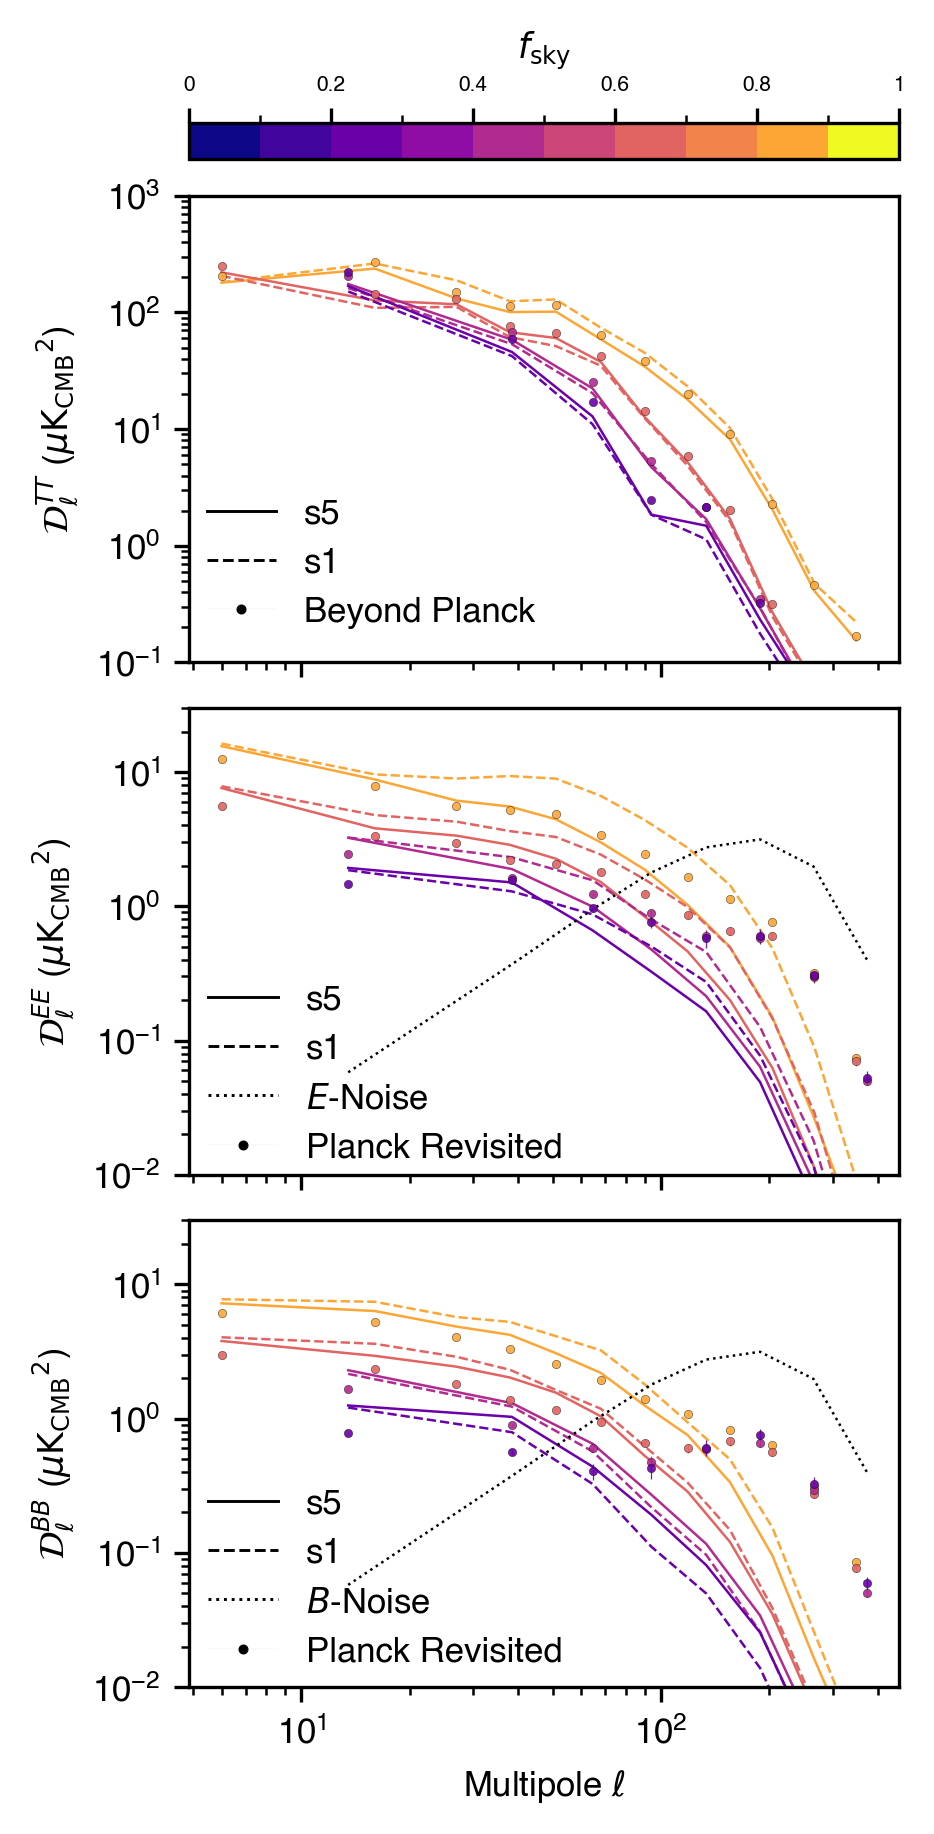
\includegraphics[width=0.48\textwidth]{figures/Dlcomp_PySM3-4_s5_vs_BPPR_SYNC.png}
    \caption{Figure showing comparison of power spectra of the PySM s5 model with observation on different sky fractions. The spectra obtained for models s4, s6 and s7 are similar so we don't show them here. The $TT$ power spectrum comparison is done with synchrotron intensity map from BeyondPlanck release 1 \citep{BeyondPlanck23} at 30 GHz with $2^\circ$ beam. The $EE$ and $BB$ power spectra is compared with Planck Revisited \citep{Delabrouille2024} polarized synchrotron map at 30\,GHz with $1^\circ$ beam. The EE and BB spectra for observations are debiased for noise, computed from 200 simulations.}
   \label{fig:Dl_sync_galmask}
\end{figure}

The $TT$, $EE$ and $BB$ power spectra comparisons, for model \texttt{s5}, are shown in Figure~\ref{fig:Dl_sync_galmask}. The comparison for models \texttt{s4}, \texttt{s6} and \texttt{s7} have nearly identical results. The $TT$ power spectra for all sky fractions show excellent agreement with the BeyondPlanck synchrotron temperature power spectra. For polarization $E$ modes, we find a good agreement with observations for all but the 20 \% sky fraction. 
% So, it is reasonable to argue that for synchrotron temperature there is excellent agreement for all but the brightest parts of the sky, where the comparison is harder to make at 30\,GHz. 
For BB spectrum, the PySM model has slightly higher power, for $\ell < 100$. The difference increases at smaller sky fractions. 
\giuse{However, such a divergence is somewhat expected as we are considering multipoles far from the injection one ($\ell\sim36$).} 
% In fact, some of the features observed in the LFI 30 GHz spectra are not found in the pysm spectra as they are by construction generated to have a power law shape.
For $\ell > 100$, we find a bump in spectrum for the observation. This is probably a combined effect of residual point sources, incorrect masking choice in $B$-mode polarization, and perhaps some residual noise.

\giuse{Moreover, an important caveat of the current synchrotron templates is that despite the point source masking, we find and excess due to Galactic point sources at low   latitudes around the Galactic center. We thus remark here that the \texttt{s4}, \texttt{s5},\texttt{s6} and \texttt{s7} models  are reliable at $\ell \lesssim 3000 $ and outside the Galactic plane. We devote to a future release the treatment of small scale structure in bright regions. }


\subsubsection{BICEP/Keck Patch}

\begin{figure*}
    \centering
    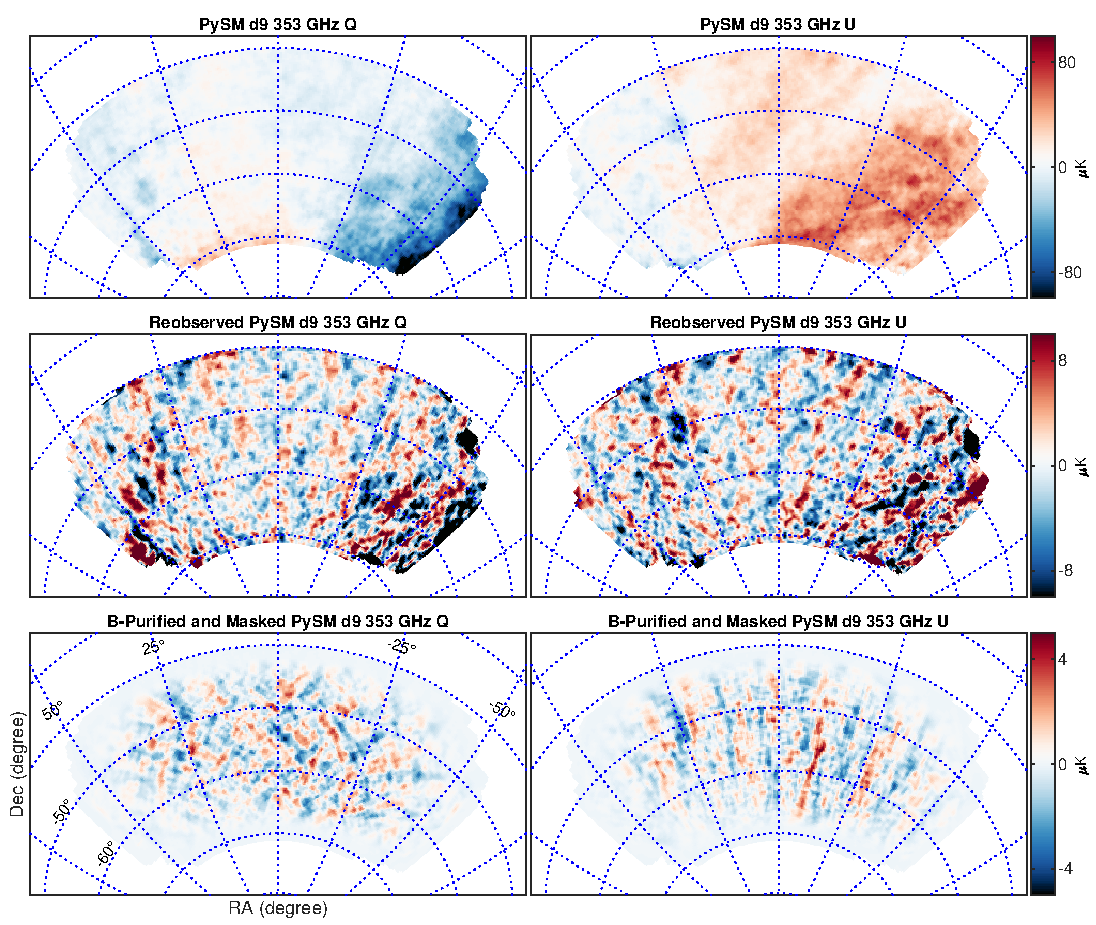
\includegraphics[width=2.\columnwidth]{figures/pysm_d9_353_delta_reobs_B_pub.pdf}
    \caption{The PySM \texttt{d9} maps, reobserved maps and purified maps in the BICEP/Keck sky patch at delta 353 GHz. Each panel shows the
    PySM $Q$/$U$ maps reprocessed by the BK18 BICEP3 beam profile, observation matrix and purification matrix respectively.}
    \label{fig:psym_BKmatrix}
\end{figure*}

The cleanest patch of sky in the southern hemisphere is particularly important for ongoing and future CMB experiments that target the primordial B-mode polarization. The strongest constraints on the tensor-to-scalar ratio to date, with an experimental uncertainty $\sigma(r) = 0.009$ and an upper limit of $r < 0.036~(95\%)$, are set by the BICEP/Keck (BK) experiment using their science data up to the 2018 season~\citep[``BK18'';][]{Ade:2021}. The constraints are derived from a combination of BK, Planck and WMAP 23--353~GHz data observed from the $\approx 600$ square degree sky patch centering at RA 0h, Dec. $-57.5^{\circ}$. Over the next few years, a collaborative effort between the South Pole Telescope (SPT) and BICEP/Keck will combine high-resolution SPT-3G observations with BICEP3 and BICEP Array observations in order to ``delens'' the observed CMB B-modes to further constrain $r$, yielding $\sigma(r) \lesssim 0.003$~\citep{2022arXiv220316556B}. As this observation field will also overlap with the tentative sky patch of the CMB-S4 experiment for their primordial B-mode search \citep{Abazajian:2022}, there will be continued interest in simulating its Galactic foregrounds, meriting a more comprehensive analysis. 

As demonstrated in Fig.~\ref{fig:psym_BKmatrix}, we apply a new method to compute the $BB$ power spectra of the PySM models in the BK sky patch before comparing them to the best measurement available. In the first panel, the PySM \texttt{d9} $Q$/$U$ maps integrated with a delta 353~GHz bandpass are masked to the BICEP3 observation region and convolved with the BICEP3 beam profile to include the beam-smoothing effect. The next panel shows the results after multiplying the BK18 BICEP3 observation matrix to these smoothed maps. As part of standard data products in the BK analysis \citep{Ade:2016}, this matrix accurately captures various timestream processing (for example the third-order polynomial filtering applied along RA scans) and beam deprojection in the linear map-making process, turning the input maps as if they are observed and analyzed through the BICEP3 telescope. These maps hence lose their large-scale structures and their color scale is decreased by 10 times. In the third panel, the intermediate maps are further multiplied by the corresponding purification matrix and the inverse noise-variance apodization mask to remove pure E-modes and ambiguous modes arising from a
filtered small-field observation, yielding two B-mode dominated $Q$ and $U$ maps with clear ``cross-like'' and ``plus-like'' pattern respectively. 

With the same process applied to other PySM models at frequencies of interest, we acquire a set of filtered and purified foreground polarization maps which represent the foreground outcomes from realistic B-mode measurements of the sky patch. We then proceed to calculate their $BB$ auto power spectra using the BK binning. In Fig.~\ref{fig:BKfield_power}, we show the \texttt{d9} and \texttt{d12} $BB$ band power at 353~GHz and the \texttt{s4}, \texttt{s5} and \texttt{s7} band power at 30~GHz. These PySM power spectra are compared with the BK18 maximum likelihood foreground model comprises a modified blackbody power spectrum ($T_d$ fixed at $19.6~\text{K}$) with parameter $A_d = 4.4 \mu\text{K}^2$ , $\beta_d = 1.5$ and $\alpha_d = -0.66$ for dust, and a square-law power spectrum with parameter $A_s = 0.6 \mu\text{K}^2$, $\beta_s = -3.0$ and $\alpha_s = 0.00$ for synchrotron\footnote{These $A_s$ and $A_d$ values are evaluated at 23~GHz and 353~GHz ($\ell = 80$) respectively.}. These BK18 model lines are suppressed by its band power window function to account for the mode loss and mode coupling induced by the observation matrix, purification matrix and binning as well. 

\begin{figure}
    \centering
    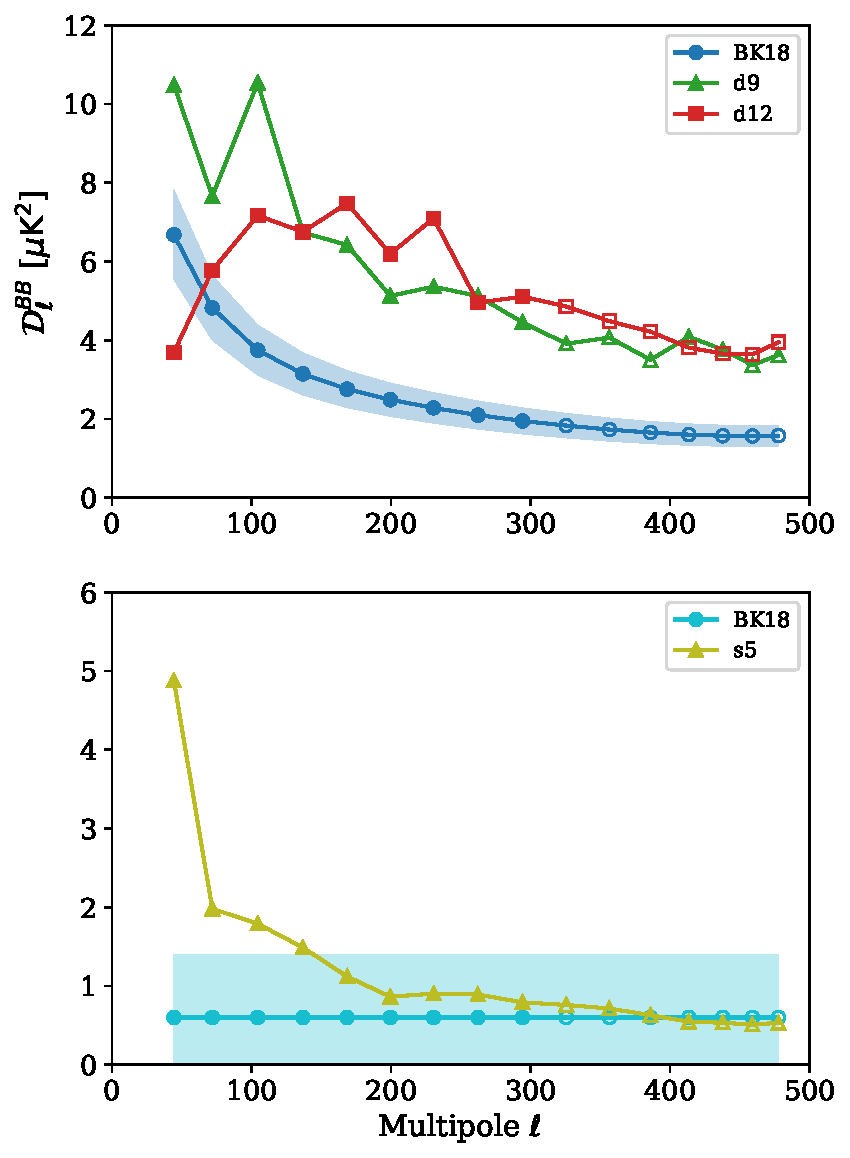
\includegraphics[width=0.48\textwidth]{figures/BKfield_power.pdf}
    \caption{Comparison between PySM $BB$ power spectra of the BK patch and the BK18 maximum likelihood models. All band power are converted to full-sky $D_\ell$ by a division of the integral of band power window function. The shaded area represents an uncertainity in foreground amplitudes ($\pm 0.75~\mu\text{K}^2$ for dust and a 95\% upper limit $1.2~\mu\text{K}^2$ synchrotron) extracted from BK18 MCMC constraints.}
    \label{fig:BKfield_power}
\end{figure}

%The current upper limit on the tensor-to-scalar ratio is set by a combination of BICEP / Keck (BK), Planck, and WMAP data: $r < 0.036~(95\%)$ \citep{Ade:2021}. Over the next few years, a collaborative effort between the South Pole Telescope (SPT) and BICEP / Keck will combine high-resolution SPT-3G observations with BK observations in order to ``delens'' the observed CMB B-modes, and further constrain $r$. Therefore, there will be continued interest in simulating Galactic foregrounds on this particular patch of sky.

... table~\ref{tab:BB_dustratio} ... 
In this comparison, 

model \texttt{d9} and \texttt{d12} clearly 

In Figure~\ref{fig:d1d9_bkpatch} we compare the BB power spectrum of the new \dnine{} model with the original PySM \done{} model, the GNILC input map, and the maximum likelihood dust model in this patch of sky determined from a combination of BK, Planck and WMAP data \citep{Ade:2021}. Model \done{} clearly has excess dust BB power compared to the measured amplitude in this patch of sky, which has been known for some time. This is somewhat ameliorated in model \dnine{}, primarily due to the steeper spectral tilt of the \dnine{} model leading to a factor of $\sim 10$ decrease in power relative to \done{} by multipoles of $\ell \gtrsim 300$. At larger scales of $\ell \lesssim 50$ both the \done{} and \dnine{} models are dominated by the underlying GNILC template, rather than the simulated small scale realizations, and so the mismatch in amplitude between the BK maximum likelihood model and our templates is most likely due to residual noise in the GNILC template. Indeed, most of the constraining power on dust BB power in Ref~\cite{Ade:2021} is driven by BK observations at 220\,GHz, which are not used to inform our model. 

%In Figure~\ref{fig:d1d9_bkpatch} we compare the BB power spectrum of the new \dnine{} model with the original PySM \done{} model, the GNILC input map, and the maximum likelihood dust model in this patch of sky determined from a combination of BK, Planck and WMAP data \citep{Ade:2021}. Model \done{} clearly has excess dust BB power compared to the measured amplitude in this patch of sky, which has been known for some time. This is somewhat ameliorated in model \dnine{}, primarily due to the steeper spectral tilt of the \dnine{} model leading to a factor of $\sim 10$ decrease in power relative to \done{} by multipoles of $\ell \gtrsim 300$. At larger scales of $\ell \lesssim 50$ both the \done{} and \dnine{} models are dominated by the underlying GNILC template, rather than the simulated small scale realizations, and so the mismatch in amplitude between the BK maximum likelihood model and our templates is most likely due to residual noise in the GNILC template. Indeed, most of the constraining power on dust BB power in Ref~\cite{Ade:2021} is driven by BK observations at 220\,GHz, which are not used to inform our model. 

\begin{table}[]
    \centering
    \begin{tabular}{lccccc}
    \toprule 
     & 85~GHz & 150~GHz & 220~GHz & 270~GHz & 353~GHz \\
    \midrule
    \texttt{d9}  & 2.17 & 2.12 & 2.08 & 2.06 & 2.03 \\
    \texttt{d10} & 0.96 & 1.30 & 1.59 & 1.77 & 2.03 \\
    \texttt{d12} & 2.76	& 2.27 & 2.08 & 2.02 & 1.96 \\
   \bottomrule
    \end{tabular}
    \caption{The deviation ratio of the reobserved PySM dust $BB$ spectrum to the BK18 best-fit modified blackbody spectrum at each delta frequency.}
    \label{tab:BB_dustratio}
\end{table}

One may argue that the amplitude of the \texttt{d9}, \texttt{d10} and \texttt{d12} model disagree with existing observations in the BK patch of sky. While this is true, it is beyond the scope of this work to provide full sky simulations that guarantee consistency with all sets of full sky and partial sky observations. Indeed, the use of power spectrum-based techniques requires a certain amount of global averaging of power spectrum parameters that are in fact known to vary across the sky \cite{planck2016-l04}. For example, while the dust amplitude can be modulated by the use of a large scale template, the spectral tilt has to be fixed to a single value for the full sky, which is not realistic. 

%One may argue that the amplitude of the \texttt{d9} and \texttt{d10} model disagree with existing observations in the BK patch of sky. While this is true, it is beyond the scope of this work to provide full sky simulations that guarantee consistency with all sets of full sky and partial sky observations. Indeed, the use of power spectrum-based techniques requires a certain amount of global averaging of power spectrum parameters that are in fact known to vary across the sky \cite{planck2016-l04}. For example, while the dust amplitude can be modulated by the use of a large scale template, the spectral tilt has to be fixed to a single value for the full sky, which is not realistic. 

%One may argue that the amplitude and spectral tilt of the \dnine{} model clearly disagree with existing observations in the BK patch of sky. While this is true, it is beyond the scope of this work to provide full sky simulations that guarantee consistency with all sets of full sky and partial sky observations. Indeed, the use of power spectrum-based techniques requires a certain amount of global averaging of power spectrum parameters that are in fact known to vary across the sky \cite{planck2016-l04}. For example, while the dust amplitude can be modulated by the use of a large scale template, the spectral tilt has to be fixed to a single value for the full sky, which is not realistic.

%\begin{table}[]
%    \centering
%    \begin{tabular}{lccc}
%    \toprule 
%     & 20~GHz & 30~GHz & 40~GHz\\
%    \midrule
%    \texttt{s4} & & & \\
%    \texttt{s5} & & & \\
%    \texttt{s7} & & & \\
%   \bottomrule
%    \end{tabular}
%    \caption{Same as table~\ref{tab:BB_dustratio} but for PySM synchrotron models.}
%    \label{tab:BB_syncratio}
%\end{table}
% 1. All models behave similarly? 
% 2. No ratio to 0 of BK18...

%\begin{figure}[ht]
%    \centering
%    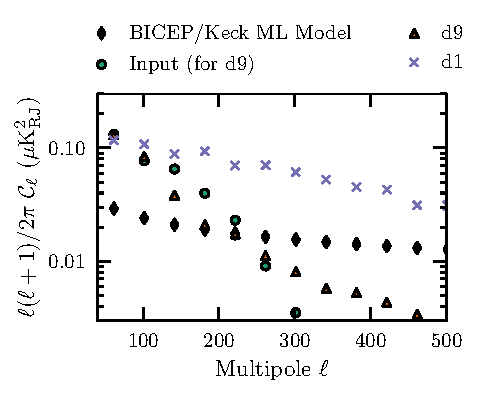
\includegraphics{paper_BK_patch.pdf}
%    \caption{This figure shows the BB power spectra of the \done{} (crosses), \dnine{} (triangles), and varres GNILC map (circles), compared to the maximum likelihood BK dust model (black diamonds) derived from a combination of WMAP and Planck with BICEP / Keck data up to the 2018 observing season. Note that in order to make a meaningful comparison between the bandpowers calculated from maps and the theory curve, we first convolve the theory spectrum with the mode-coupling matrix and then compute the decoupled bandpowers by applying the inverted binned coupling matrix.}
%    \label{fig:d1d9_bkpatch}
%\end{figure}

%The cleanest patch of sky in the southern hemisphere is particularly important for ongoing and future CMB experiments that target measurement of the primordial CMB B-modes. We focus on the small clean patch of sky that is targeted for the BICEP/Keck experiment for their constraints on the tensor-to-scalar ratio. This overlaps with the tentative sky patch that will be targeted by the CMB-S4 experiment for their primordial B-mode search \citep{Abazajian:2022}. In their 2021 analysis the BICEP/Keck team placed a upper limit of $A_s<1.4 \mu{\rm K}^2$ at a pivot frequency of 23\,GHz with $\beta_s=-3.1$ after marginalizing over the range $-1<\alpha_s<0$ \citep{Ade:2021}. The BICEP/Keck maximum likelihood model for the synchrotron spectrum is parameterized by $A_s=0.6 \mu{\rm K}^2$, $\beta_s=-3.0$ and $\alpha_s=0$. 
% In Figure~\ref{fig:Dl_sync_BK}, we compare these two sets of constraints from the BICEP/Keck 2018 results with the new PySM synchrotron models s4, s5 and s7. We also plot the old PySM s1 synchrotron model to show how the synchrotron model has changed in this patch of interest.

The new synchrotron models, s4, s5 and s7, have more power in the BICEP/Keck patch when compared to the old s1 synchrotron model. The latest BICEP/Keck results only has weak detection of synchrotron. We find that both the old and new PySM models are consistent with the BICEP/Keck upper limit on the synchrotron power. However, the BICEP/Keck maximum likelihood model for synchrotron has a better agreement with the new synchrotron models s4, s5 and s7 than with the old s1 synchrotron model. Thus, the new small scale generation in the synchrotron models s4, s5, and s7 increases the synchrotron power in the BICEP/Keck patch and is in better agreement with the constraints from the latest BICEP/Keck results.

\subsection{Decorrelation}

In this section, we compare the decorrelation properties of various models, computed on the Galactic masks of the previous Section. The decorrelation parameter

\begin{equation}
    \mathcal{R}^{XY}_\ell(\nu_1\times\nu_2) = \frac{\mathcal{D}_\ell^{XY}(\nu_1\times\nu_2)}{\sqrt{\mathcal{D}_\ell^{XY}(\nu_1\times\nu_1)\mathcal{D}_\ell^{XY}(\nu_2\times\nu_2)}}
\end{equation}
\giuse{\bf We need to complete this section !  }
Myra Norton's decorrelation plot to go here. Github: https://github.com/galsci/pysm/issues/123

\subsection{Extragalactic contamination}

\label{sec:CIBcontamination}

%[Stanford student Monica Hicks is working with Susan on cross-correlating our models with galaxy surveys a la Chiang \& Menard.] 

\begin{figure}[h!]
    \centering
    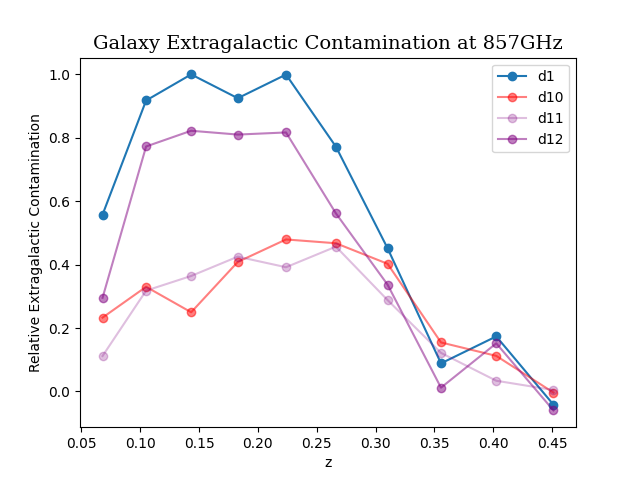
\includegraphics[width=\columnwidth]{figures/EGC_galaxy@857Part_0-1.png}
    \caption{Relative extragalactic contamination in three of the new dust templates (\texttt{d10, d11, d12}), compared to the \texttt{d1} model. Contamination is quantified as the excess 857 GHz emission within $11'$ of galaxies from the GLADE+ catalog, normalized to the maximum excess and plotted as a function of redshift (z). All three new dust templates contain less extragalactic contamination than older dust models because they are based on GNILC-processed Planck data. The improvement is most significant for \texttt{d10} and \texttt{d11}.  }
    \label{fig:extragal_contamination}
\end{figure}


%Our Galactic dust templates are based on measurements of the 
We quantify the extragalactic contamination present in our dust models using a tomographic redshift-clustering technique \citep{Schmidt:2015, Chiang:2019}. Our intensity-based Galactic dust templates inevitably contain emission from both Galactic dust and external galaxies. As described in Section \ref{sec:dustamplitude}, the new \texttt{d9} and \texttt{d10} dust templates are derived from GNILC-processed Planck data, while older PySM dust templates used \texttt{Commander} data products. We thus expect that the new Galactic dust models are significantly less affected by CIB contamination than previous models. Here we quantify this contamination by measuring the angular cross-correlation between our dust models and the clustering of galaxies as a function of redshift in spectroscopic survey data. A perfect Galactic dust template would be uncorrelated with such clustering; the signature of CIB contamination is excess template emission correlated with galaxy clustering. 

Following the procedure in \citet{Chiang:2019}, we compute the cross-correlation between local fluctuations in the Galactic emission maps and the galaxy density as a function of redshift, using galaxies from the GLADE+ catalog \citep{Dalya:2022}. We compute this cross-correlation for each of the \texttt{d1, d10, d11}, and \texttt{d12} dust emission templates at 857 GHz, at high Galactic latitudes ($\left|b\right| > 30\deg$). Figure \ref{fig:extragal_contamination} shows that while each of the new GNILC-based maps contain less extragalactic contamination than \texttt{d1}, the decreased contamination is more marked in \texttt{d10} and \texttt{d11} than in \texttt{d12}. This is likely due to [FILTERING CHOICES? TO DISCUSS WITH JACQUES]


\subsection{Non-Gaussianity} \label{sec:nongaussianity}

In this section, we quantify the level of non-Gaussianity in the small-scale dust emission generated through the polarization fraction tensor transformation using the simulations from PySM dust model \deleven. Since small-scale fluctuations in the new synchrotron emission maps were constructed following the same algorithm (Section~\ref{sec:small_scales}), we expect those maps to show similar levels of non-Gaussianity. To measure the non-Gaussianity in the maps we use the Minkowski Functionals \citep[MFs][]{Minkowski1903}, which are regularly used to quantify map-space non-Gaussianity in the cosmology literature \citep{Martire:2023, Carones:2024}. Hadwiger’s theorem \citep{hadwigerVorlesungenUeberInhalt1957} implies that, for any $n$-dimensional excursion set defined with a threshold value $\rho$, there exist $n+1$ MFs that geometrically and topologically describe the morphology of the set. In our case, for two-dimensional maps, we have three kinds of MFs, $\mathcal{V}_0$, $\mathcal{V}_1$ and $\mathcal{V}_2$ which correspond to the area, the perimeter and the connectivity of the excursion set, respectively.

We use these MFs to compare the small-scale structure in \deleven\ to synthesized Gaussian random fields with the same power spectra as the \deleven\ maps.
%By comparing the MFs of the small-scale structures from \deleven\ with those of Gaussian realizations from extrapolated power law, which is fitted from the power spectra of the maps from \deleven{}, in standard $IQU$ domain, we can have a qualitative estimation of non-Gaussianity in \deleven{} introduced by going into $iqu$ domain.
As mentioned in Section~\ref{subsec:methodology}, the generated small scales in the \deleven\ model are modulated before they are added to the large scale template. Anisotropy in the large-scale templates might therefore introduce small-scale non-Gaussianity to the maps via this modulation. %To study the potential effect of anisotropy on the non-Gaussianity, we also generate Gaussian realizations with modulation so that we can compare the non-Gaussianity directly, without the influence of anisotropy.
To isolate the non-Gaussianity of the small-scales, we also generate Gaussian random realizations that are modulated to have the same anisotropy as the small-scale \dnine\ and \deleven\ maps. The two reference sets made of pure Gaussian small scales and modulated Gaussian small scales are built as follows:

\begin{enumerate}

\item We first fit power laws to the $TT$, $EE$, $BB$ power spectra in the multipole range $[800, 2000]$ calculated from the \deleven\ maps with the \texttt{GAL097} mask, and we synthesize Gaussian random fields that have the fitted power law out to ell = $\ell_{\rm max}=4096$. 

\item To obtain only the small scales, we apply a high-pass filter to the fitted power law with $\ell_{cut} = 200$ for intensity and polarization maps, and then generate full sky small scales realizations from the truncated power law using \texttt{synfast} routine provided by HEALPix. 

\item For modulated Gaussian maps, the full-sky small-scale structure realizations are then multiplied with modulation maps to have similar anisotropies with the small scales from \deleven{}. %We do not modulate the pure Gaussian maps. 

%\item Meanwhile, the small scales with multipoles larger than 200 in the observed data are filtered out and the large scales remain untouched.

\item Finally, the two sets of generated Gaussian small scales (modulated and unmodulated) are added to the large-scale dust template to form the final set of maps.
\end{enumerate}

Now we have three sets of maps with different small scales co-added: model \deleven, a map with purely Gaussian small-scale structure, and a map with modulated Gaussian small-scale structure. %and the last from modulated Gaussian realization in the $IQU$ domain.
We apply a high-pass filter to retain only the small scales of these maps, which we will refer to as \texttt{poltens-ss}, \texttt{Gaussian-mod-ss}, and \texttt{Gaussian-ss}, respectively. We calculate the MFs both on the sphere and in several select regions of the sky projected into a Cartesian projection. Note that the design of the modulation maps is to ensure the final \texttt{Gaussian-mod-ss} maps have the same anisotropy as \texttt{poltens-ss}, which is done by tuning the modulation maps to let \texttt{Gaussian-mod-ss} have the same power spectra behavior as \texttt{poltens-ss} on different masks that exclude the inner part of the Galactic plane. \texttt{Gaussian-ss} are fully Gaussian and isotropic since they are built from texttt{synfast} routine without any further processing . 

%Below we show the MFs calculated for these three sets of small scales on the sphere and also for a selected flat patch.

\subsubsection{Minkowski Functionals on the sphere}

Following the algorithm in \cite{Grewal:2022}, we calculate the MFs for the three $Q$ maps on the sphere, i.e., HEALPix format, with a \texttt{GAL080} mask \footnote{\url{http://pla.esac.esa.int/pla/aio/product-action?MAP.MAP_ID=HFI_Mask_GalPlane-apo2_2048_R2.00.fits}}, which masks out the Galactic plane. We first normalize the maps by dividing each map by its standard deviation and retain only pixels with values $[-3, 3]$ over which to calculate the MFs. Results are shown in Figure~\ref{fig:MF:sphere}. The MFs of the corresponding $U$ maps look very similar to $Q$ maps and are not shown here.

Figure~\ref{fig:MF:sphere} shows that when averaging over a large sky area, the MFs of \texttt{Gaussian-mod-ss} and \texttt{poltens-ss} are almost identical, while the MFs of \texttt{Gaussian-ss} differ substantially. The difference in MFs between \texttt{poltens-ss} and \texttt{Gaussian-ss} implies the existence of non-Gaussianity in \texttt{poltens-ss}, but the similarity between \texttt{poltens-ss} and \texttt{Gaussian-mod-ss} demonstrates that the non-Gaussianity in \texttt{poltens-ss} comes from the anisotropy in the maps, which originates from the modulation, rather than from the polarization fraction tensor transformation.

\begin{figure*}[hbt!]
    \centering
    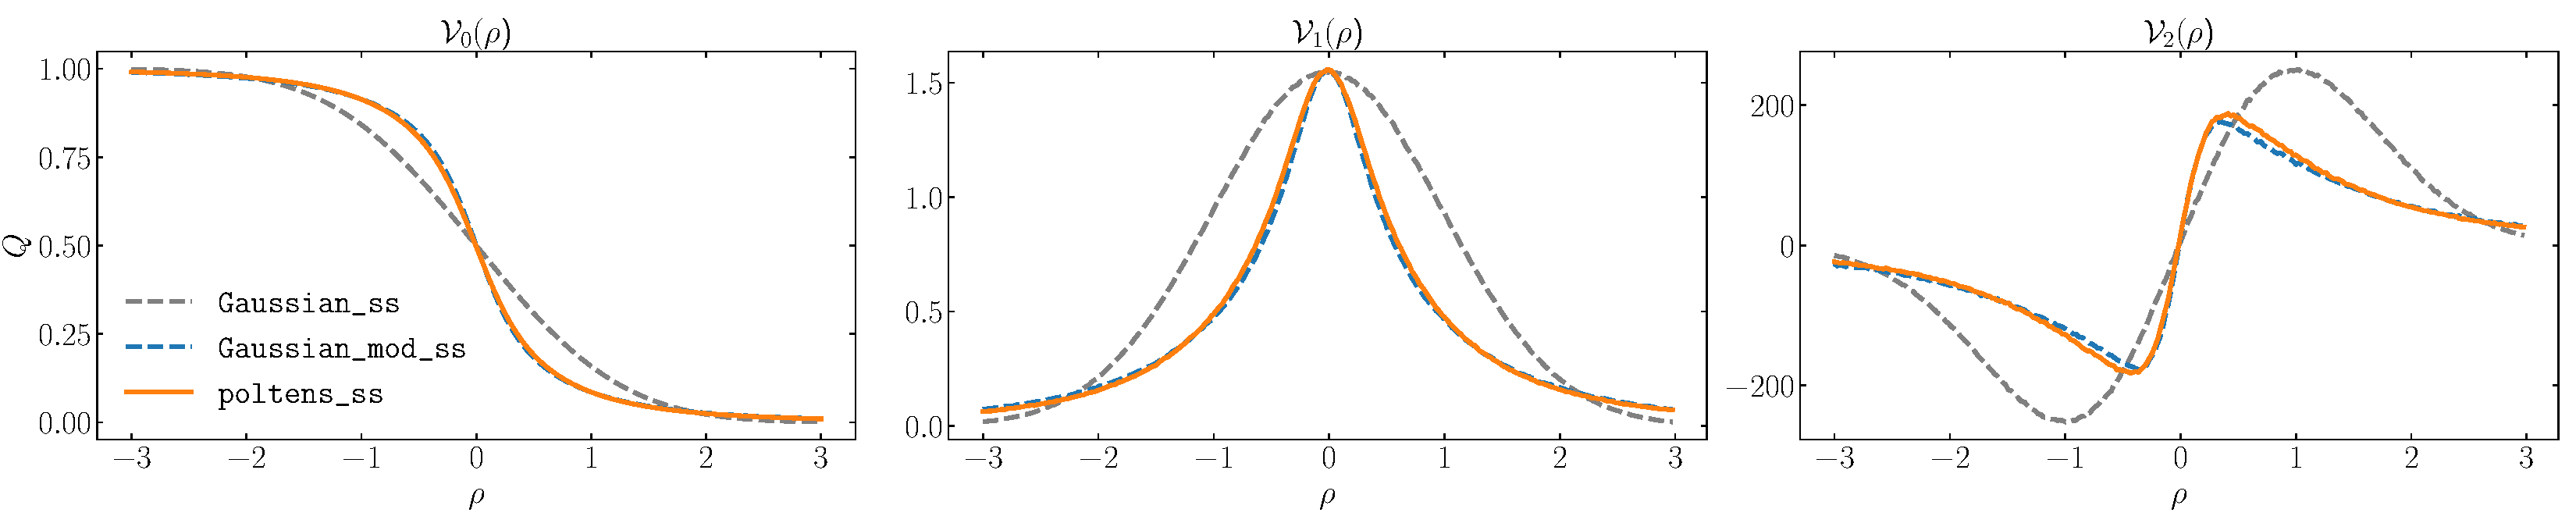
\includegraphics[width=180mm]{figures/MFs_80p_sky_Q.pdf}
    \caption{MFs for the small scales of three sets of maps on the sphere with Planck HFI 80\% mask. The small scales are filtered out by excluding multipoles $\ell < 200$ in the maps, and we choose $lmax = 2048$ when obtaining the small scales. We show the MFs as a function of threshold $\rho$, for \texttt{Gaussian-mod-ss} in blue, \texttt{poltens-ss} in orange and \texttt{Gaussian-ss} in dashed gray.}
    \label{fig:MF:sphere}
\end{figure*}

\subsubsection{Minkowski Functionals on small regions}
We consider a region centered at $(l, b) = (-15^{\circ}$, $45^{\circ})$ with dimension of $20^{\circ}\times20^{\circ}$ to determine whether significant differences in the MFs between \texttt{Gaussian-mod-ss} and \texttt{poltens-ss} sets of maps exist in small regions of sky. Those maps are shown in Figure~\ref{fig:maps:patch2}. We can see by eye that \texttt{poltens-ss} contains structure that is not present in the \texttt{Gaussian-mod-ss} maps. We calculate the MFs of these small-scale maps, following \cite{Mantz:2008} for the calculation of MFs for a square patch. Before the calculation, we also rescale all the small scales to be in the range [-1, 1].

Figure~\ref{fig:MF:patch2} shows the MFs of the \texttt{Gaussian-mod-ss} and \texttt{poltens-ss} maps presented in Figure~\ref{fig:maps:patch2}. In contrast with the large-area results presented in Figure~\ref{fig:MF:sphere}, in this case we do measure a departure of the \texttt{poltens-ss} MFs from the \texttt{Gaussian-mod-ss} ones. %This points towards the fact that the polarization fraction tensor transformation may indeed have induced some level of non-Gaussianity, distinct from pure modulation effects, that are detectable on small sky regions. 
This means that the polarization fraction tensor transformation introduced non-Gaussian small-scale structure, distinct from pure modulation effects, that is detectable on small sky regions. 
We conclude that the level of induced non-Gaussianity differs from one region to the other and does not significantly impact the statistical properties when averaged over large sky fractions.

\begin{figure*}[hbt]
    \centering
    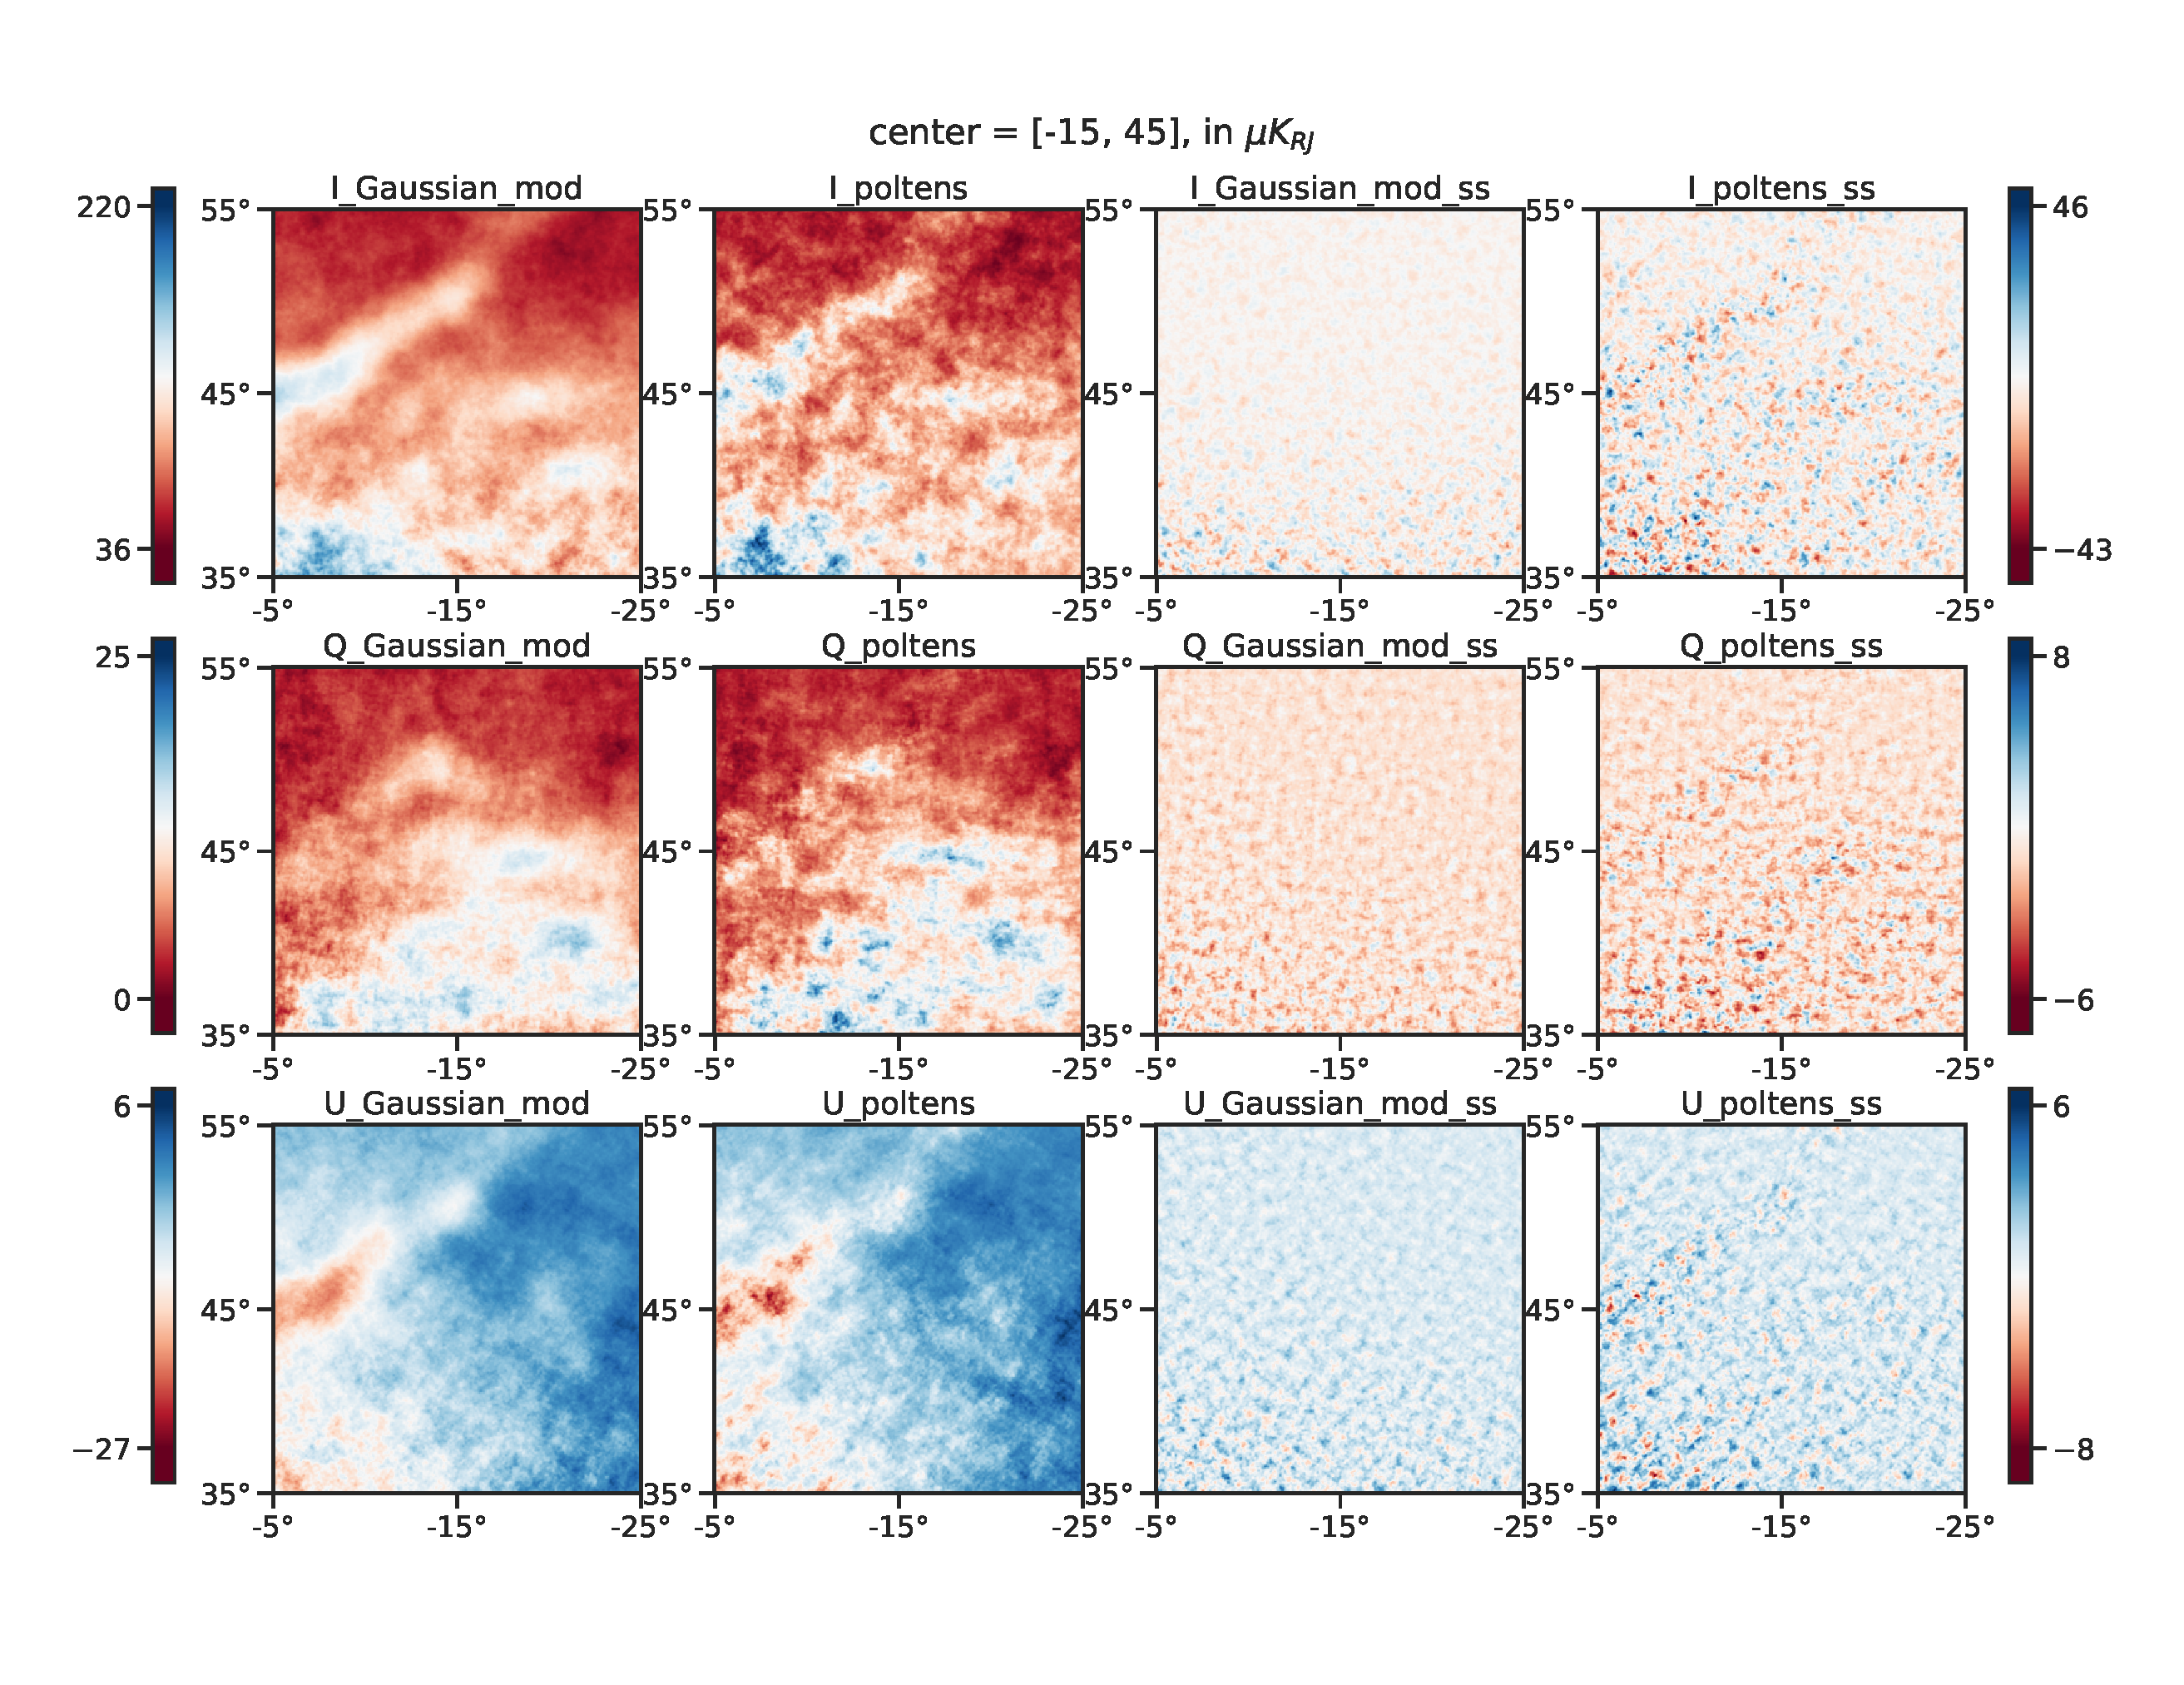
\includegraphics[width=180mm]{figures/maps_patch_345_35.pdf}
    \caption{The zoom-in plot of the maps, in the selected patch with center [$-15^{\circ}$ , $45^{\circ} $]. From left to right, we show the final map with \texttt{Gaussian-mod-ss}, final map with \texttt{poltens-ss}, \texttt{Gaussian-mod-ss} only map and \texttt{poltens-ss} only map. From top to bottom is for I, Q and U respectively. The colorbar on the left indicates the pixel values in the left-most two columns in the units of $\mu K_{RJ}$ and the colorbar on the right is for the last two columns. }
    \label{fig:maps:patch2}
\end{figure*}
\begin{figure*}[hbt]
    \centering
    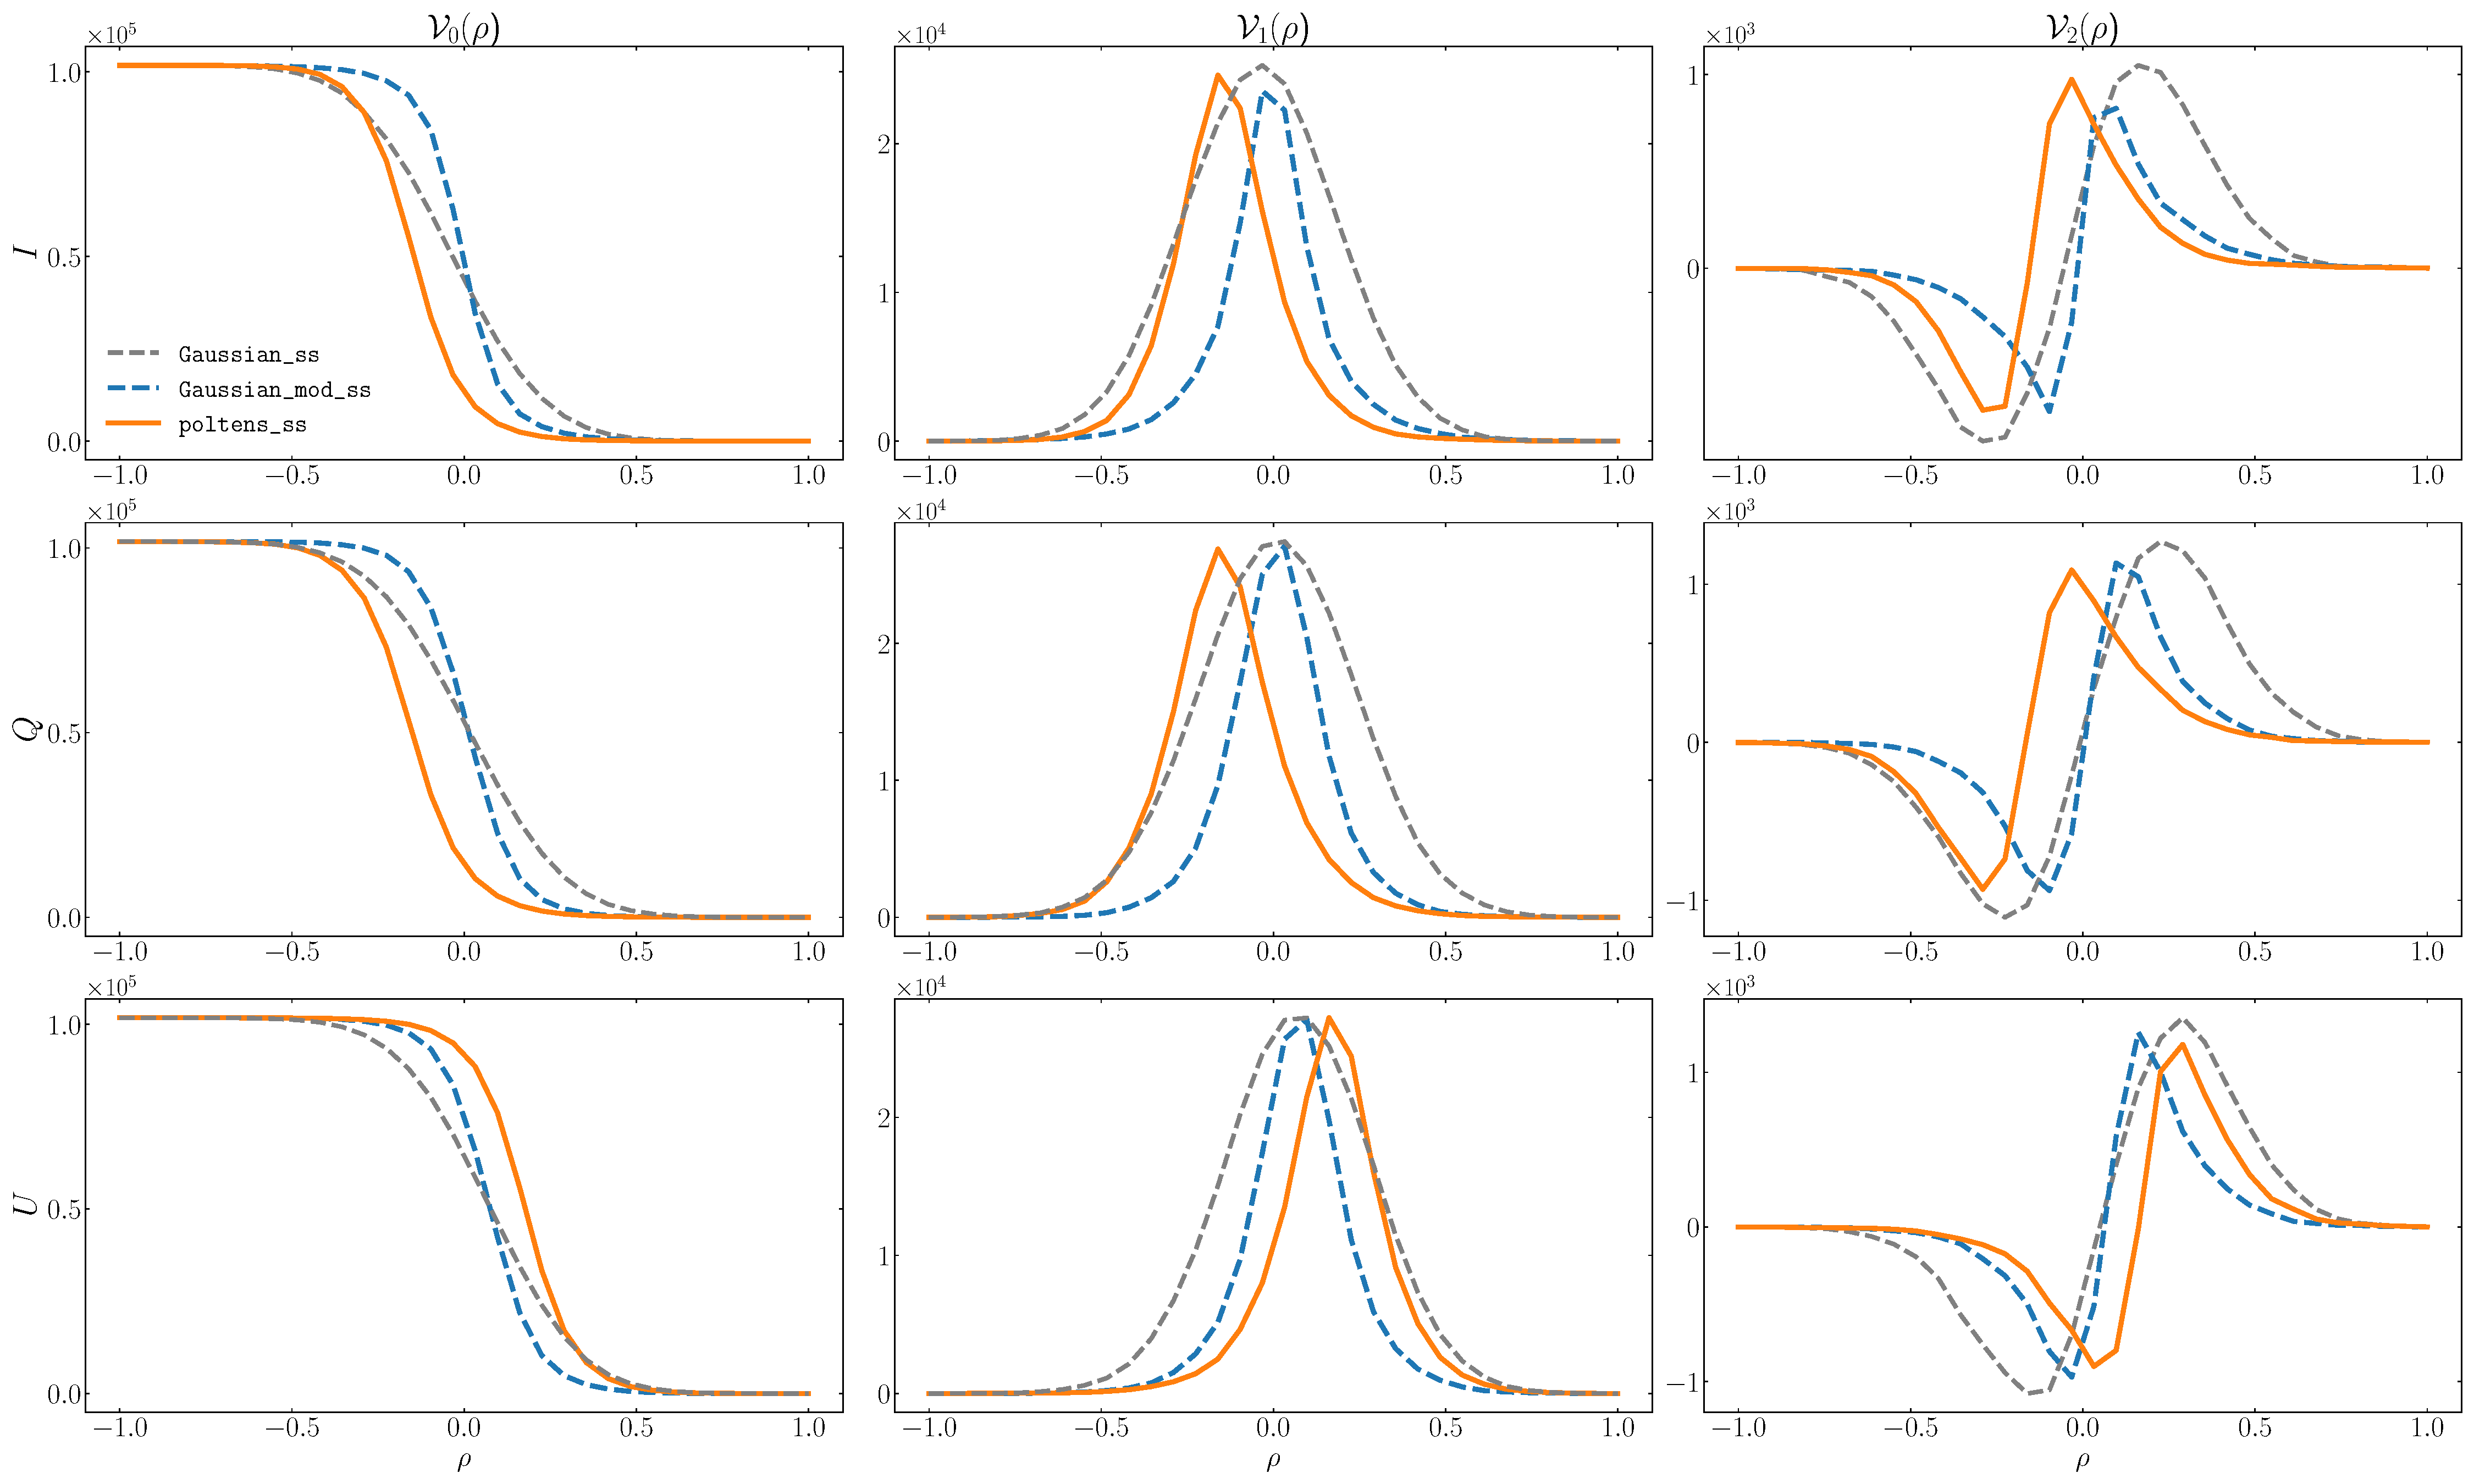
\includegraphics[width=180mm]{figures/MFs_345_45_with_G_rescaled.pdf}
    \caption{Minkowski Functionals as a function of the threshold $\rho$ for the one realization of I, Q and U small scales in the patch with center of [$-15^{\circ}$ , $45^{\circ} $] in Galactic coordinates. Each row shows three kinds of Minkowski Functionals. The blue dotted one is for \texttt{Gaussian-mod-ss} while the orange solid one is from \texttt{poltens-ss}. We also show the \texttt{Gaussian-ss} in dashed gray line as a comparison.}
    \label{fig:MF:patch2}
\end{figure*}

% BH: The commented text below has been moved, but retained here for reference + original comments
% \subsection{Synchrotron validation} \label{sec:sync_validation}
% \textbf{Shamik:} \giuse{\sout{In this section we detail the validation of the new synchrotron models by comparing them with BeyondPlanck synchrotron map for temperature, and LFI 30\,GHz observations for polarization.}}  We compare the model with data at both  map and power spectrum  levels. For validating the PySM synchrotron temperature models, we use the synchrotron map from the BeyondPlanck re-analysis of Planck LFI data \citep{Anderson2023}. BeyondPlanck released a synchrotron map\footnote{https://beyondplanck.science/products/files\_v1} at a reference frequency of 30\,GHz and at $2^\circ$ angular resolution. We produce single frequency temperature maps for the different synchrotron models at 30\,GHz and smoothed with a Gaussian beam with FWHM = $2^\circ$.

% \giuse{In case of the synchrotron polarization, we  compare the models with band integrated observations. So, we compute bandpass integrated maps  with PySM~3 routines and for  the different synchrotron models. For the sake of fair comparison with \emph{Planck} data, we adopt the average LFI 30\,GHz RIMO transmission \citep{planck2014-a03}.} The bandpass integrated maps are further smoothed with Gaussian beams of 33.1 arcmin beams to produce model maps at native resolutions of the LFI 30 GHz data. Finally, the observed power spectra are computed by taking the cross-spectrum between independent detector splits, e.g. A and B, of the NPIPE \footnote{Publicly available through NERSC at \\ /global/cfs/cdirs/cmb/data/planck2020} (PR4) 30\,GHz maps \citep{planck2020-LVII}. 

% %\subsubsection{Galactic masks}
% \giuse{We estimated the synchrotron power spectra considering three choices of masks:  full sky  (100\%), 70\% and 50\% sky fractions. To produce the masks for the latter cases, we use the LFI 30\,GHz map of polarized intensity, smoothed with a Gaussian beam of $2^\circ$ FWHM, and masked all the pixels larger than  17 and 10 $\mu{\rm K}_{\rm CMB}$, and they are shown in Figure \ref{fig:sync_masks}.  Masks are apodized  with a $2^\circ$ cosine apodization.}
% \begin{figure}
%     \centering
%     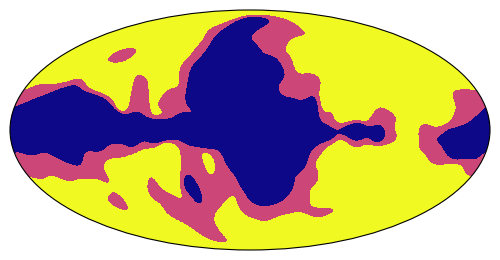
\includegraphics[width=0.46\textwidth]{figures/sync_galactic_mask.png}
%     \caption{Figure showing the two different Galactic masks used for the synchrotron validation. The yellow region is included by the 50\% sky mask, while the 70\% mask additionally includes the pink region.}
%     \label{fig:sync_masks}
% \end{figure}

% We use HEALPix \footnote{https://healpix.sourceforge.io} \texttt{anafast} function \citep{2005ApJ...622..759G, 2019JOSS....4.1298Z}  to compute the power spectra for the model and observation maps. For the polarization analysis, both the model and the LFI maps are additionally masked with the apodized LFI DR2 polarized point source mask. 
% For this validation test, we
% do not use a pseudo-$C_\ell$ estimator as the synchrotron signal is not statistically isotropic, and we correct for the partial sky by naively dividing by an $f_{\rm sky}$ factor.

% \begin{figure}
%     \centering
%     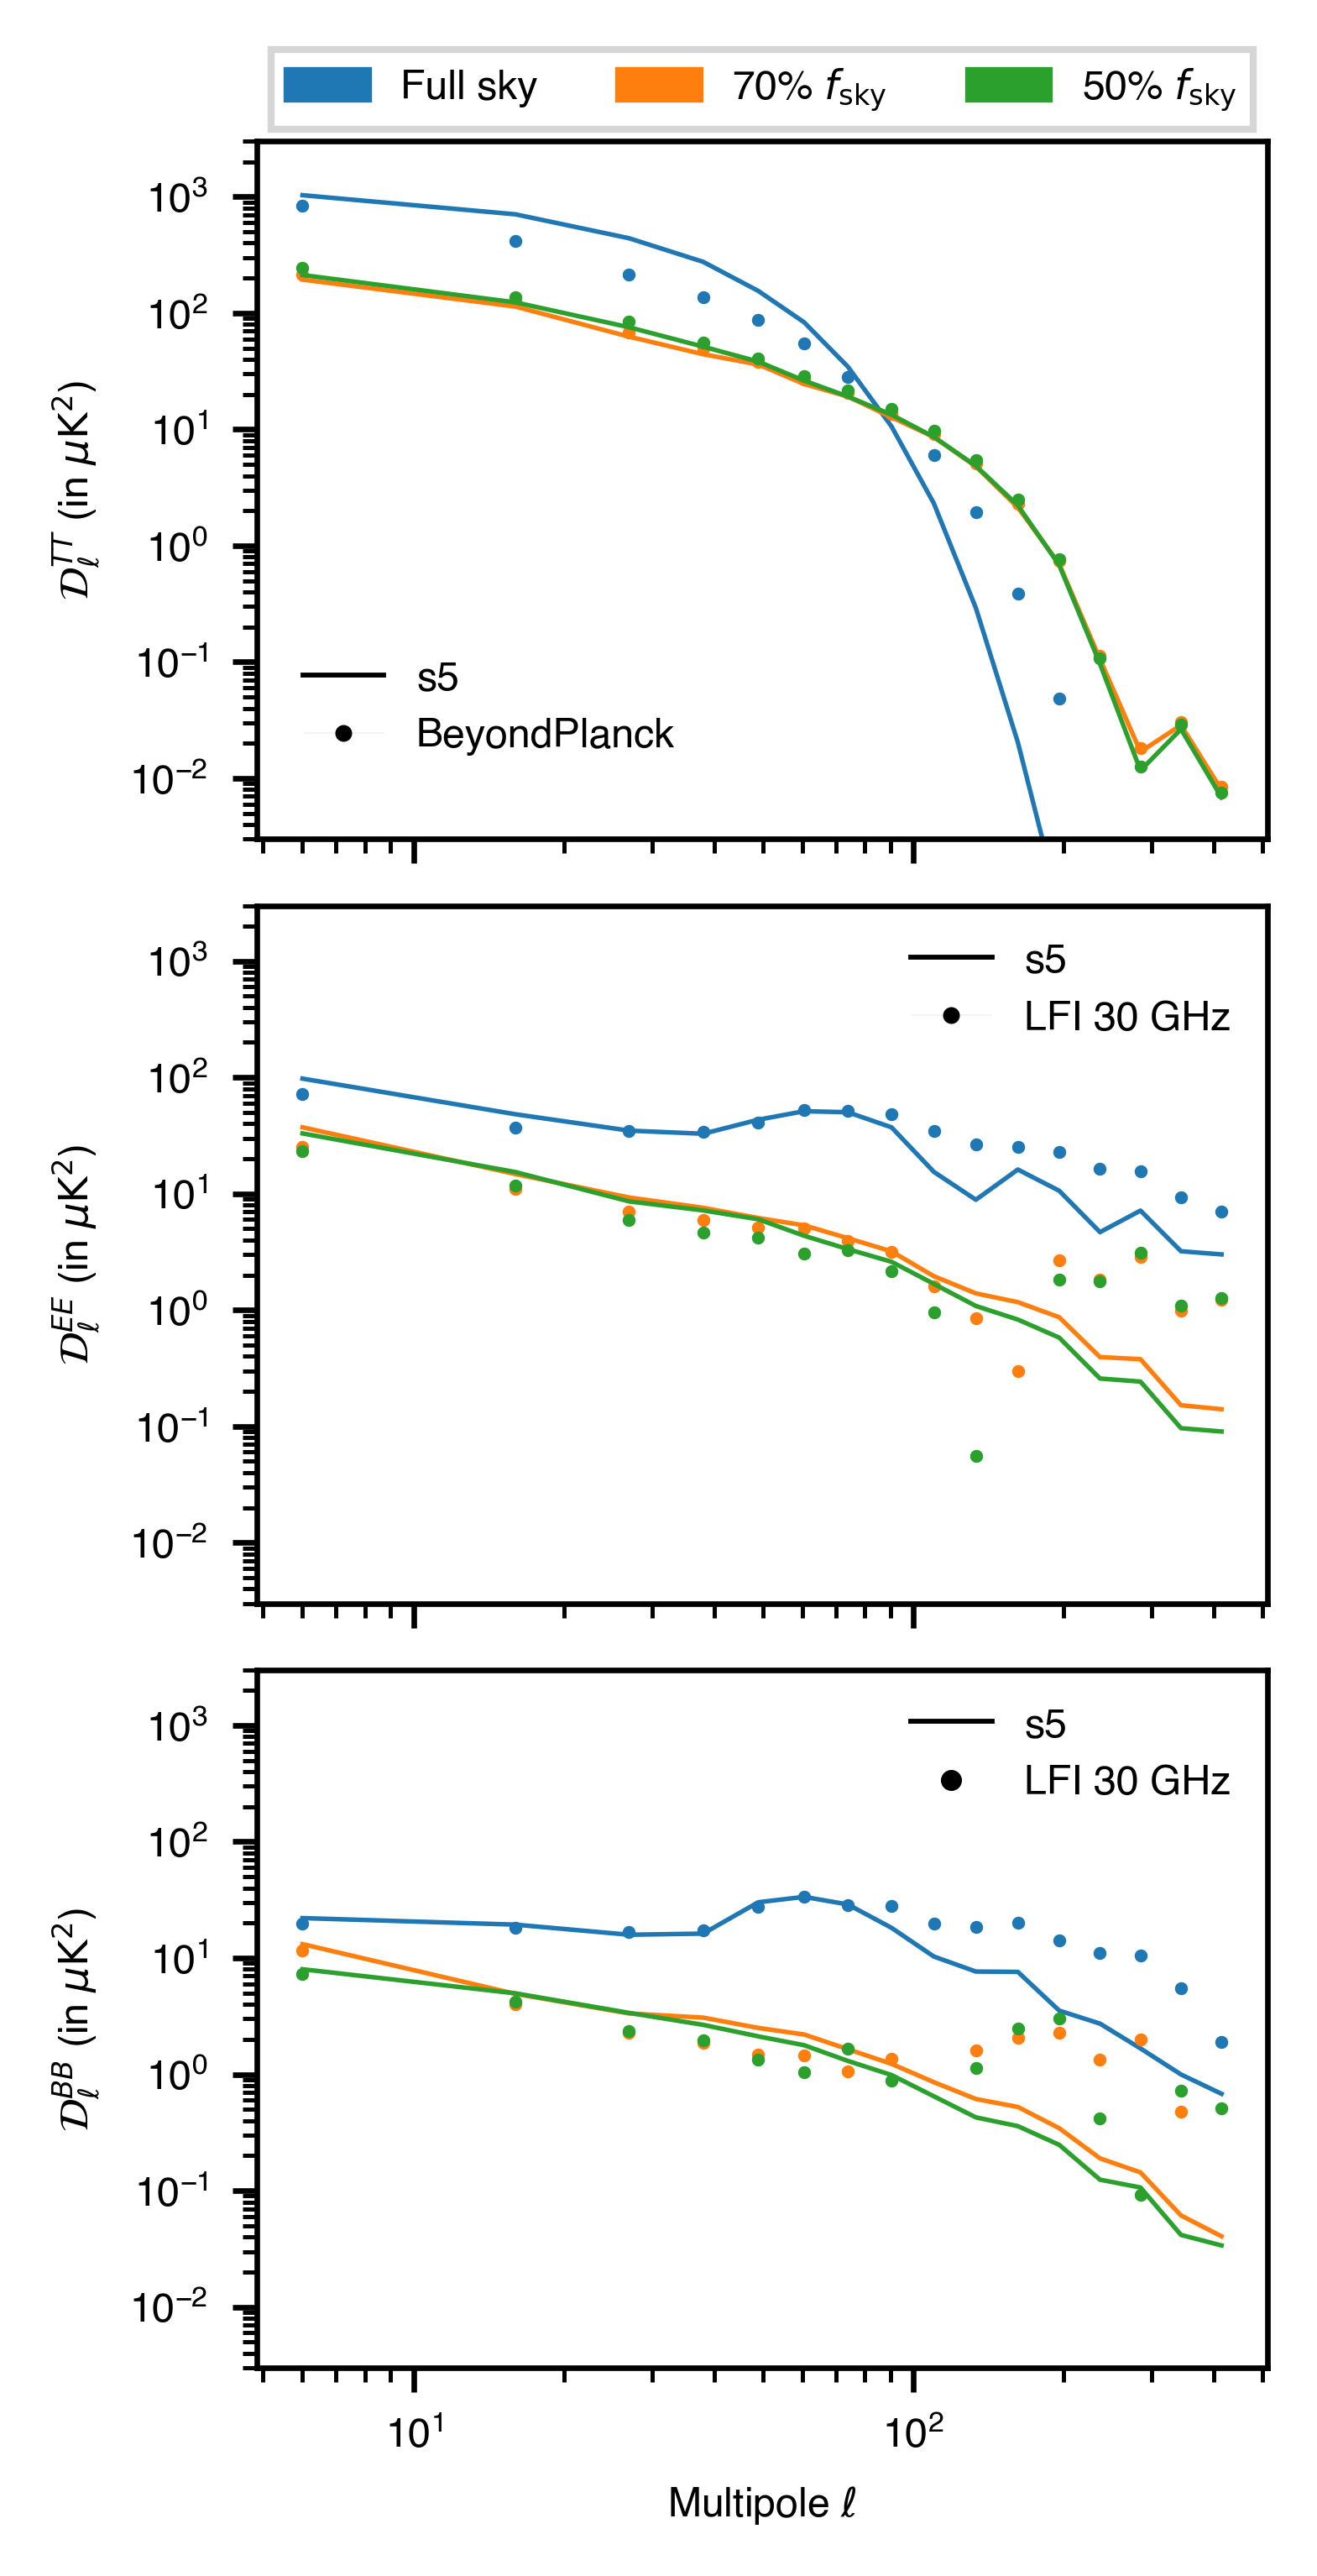
\includegraphics[width=0.48\textwidth]{figures/Dlcomp_PySM3-4b7_s5_vs_BPnLFI30_BPI.png}
%     \caption{Figure showing comparison of power spectra of the PySM s5 model with observation on different sky fractions. The spectra obtained for models s4, s6 and s7 are similar so we don't show them here. The $TT$ power spectrum comparison is done with synchrotron maps from BeyondPlanck release 1 \citep{Anderson2023}. The $EE$ and $BB$ power spectra is compared with NPIPE LFI 30\,GHz map \citep{planck2020-LVII}. The LFI 30\,GHz spectra are computed as a cross spectra between the NPIPE splits A and B.}
%     \label{fig:Dl_sync_galmask}
% \end{figure}

% The $TT$, $EE$ and $BB$ power spectra comparisons, for model s5, are shown in Figure~\ref{fig:Dl_sync_galmask}. The comparison for models s4, s6 and s7 have nearly identical results. The $TT$ power spectra for masked skies show excellent agreement with the BeyondPlanck synchrotron temperature power spectra. However, there is poor agreement for the full sky power spectra. On the full sky most of the spectra is dominated by what happens in the Galactic plane, which for observational data is contaminated by free-free and AME. Even with the BeyondPlanck component separation, the synchrotron power in the brightest sky regions is likely to have some residual contamination and associated uncertainty. The new PySM synchrotron models are difficult to assess in the regions of brightest galactic synchrotron emission and we caution users against using the synchrotron models in the brightest parts of the galaxy. However, going away from the galactic plane, we find excellent agreement with observations at power spectrum level.
% % So, it is reasonable to argue that for synchrotron temperature there is excellent agreement for all but the brightest parts of the sky, where the comparison is harder to make at 30\,GHz. 
% For polarization we find reasonable agreement at $\ell \lesssim 100$. For $\ell > 100$ the PySM synchrotron models typically have less power than the data. However, an important caveat is that despite the point source masking, there is some residual radio point source contribution to this power in the LFI maps.

% \begin{figure}
%     \centering
%     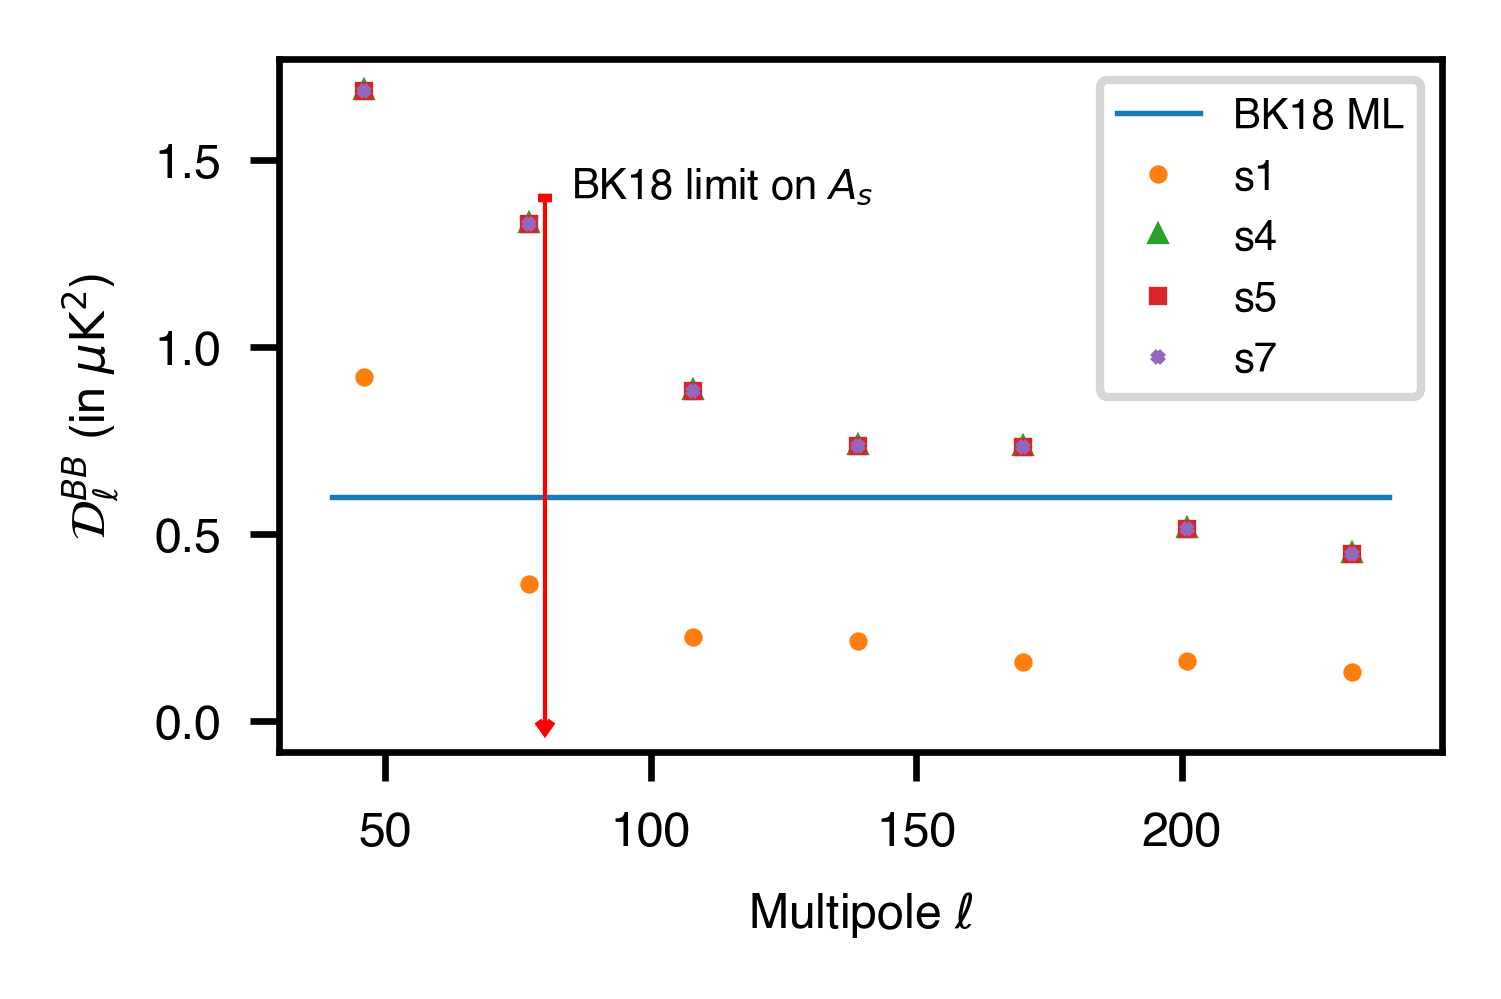
\includegraphics[width=0.49\textwidth]{figures/Dlcomp_PySM3-4b8_BKpatch.png}
%     \caption{Comparison of power spectra in the BICEP/Keck patch for the new PySM synchrotron models s4, s5 and s7 with old synchrotron model s1 and the limits on the synchrotron power obtained in BICEP/Keck 2018 \citep{Ade:2021} at the reference frequency of 23\,GHz. The blue line is the BICEP/Keck 2018 maximum likelihood model for synchrotron with $A_s=0.6 \mu {\rm K}^2$, $\alpha_s=0$. The red arrow indicates the BICEP/Keck 95\% confidence upper limit on $A_s<1.4 \mu {\rm K}^2$ after marginalizing over $-1<\alpha_s<0$ at $\ell=80$. The PySM synchrotron models s4, s5 and s7 have identical power spectra at 23\,GHz.}
%     \label{fig:Dl_sync_BK}
% \end{figure}

% \subsubsection{BICEP / Keck patch}
% The cleanest patch of sky in the southern hemisphere is particularly important for ongoing and future CMB experiments that target measurement of the primordial CMB B-modes. We focus on the small clean patch of sky that is targeted for the BICEP/Keck experiment for their constraints on the tensor-to-scalar ratio. This overlaps with the tentative sky patch that will be targeted by the CMB-S4 experiment for their primordial B-mode search \citep{CMB-S4:2020}. In their 2021 analysis the BICEP/Keck team placed a upper limit of $A_s<1.4 \mu{\rm K}^2$ at a pivot frequency of 23\,GHz with $\beta_s=-3.1$ after marginalizing over the range $-1<\alpha_s<0$ \citep{Ade:2021}. The BICEP/Keck maximum likelihood model for the synchrotron spectrum is parameterized by $A_s=0.6 \mu{\rm K}^2$, $\beta_s=-3.0$ and $\alpha_s=0$. In Figure~\ref{fig:Dl_sync_BK}, we compare these two sets of constraints from the BICEP/Keck 2018 results with the new PySM synchrotron models s4, s5 and s7. We also plot the old PySM s1 synchrotron model to show how the synchrotron model has changed in this patch of interest.

% The new synchrotron models, s4, s5 and s7, have more power in the BICEP/Keck patch when compared to the old s1 synchrotron model. The latest BICEP/Keck results only has weak detection of synchrotron. We find that both the old and new PySM models are consistent with the BICEP/Keck upper limit on the synchrotron power. However, the BICEP/Keck maximum likelihood model for synchrotron has a better agreement with the new synchrotron models s4, s5 and s7 than with the old s1 synchrotron model. Thus, the new small scale generation in the synchrotron models s4, s5, and s7 increases the synchrotron power in the BICEP/Keck patch and is in better agreement with the constraints from the latest BICEP/Keck results.

% \subsection{Dust validation} \label{sec:dust_validation}

% \textbf{Ben:} In this section we calculate the power spectra of the dust template described in Section~\ref{sec:small_scales} using a variety of Galactic masks derived for the analysis of Planck data. We also present power spectra calculated on the region of sky observed by the BICEP Array and SPT-3G experiments. This latter case will assess how the small scale model performs in small areas of high latitude sky, which are vital for future constraints on the tensor-to-scalar ratio. Primarily, we will demonstrate that the spatial modulation of the small-scale realizations does not add too much foreground power in areas of high latitude sky, which has been a criticism of previous PySM models. 

% All power spectra in this section are computed using the {\tt NaMaster} code \citep{Alonso:2019}. 

% \subsubsection{Planck Galactic masks} \label{sec:galactic_spectra}

% \textbf{Ben:} In this section we present power spectra computed on Galactic masks of varying sizes. We define a set of Galactic masks starting from the unapodized Galactic masks\footnote{\texttt{HFI\_Mask\_GalPlane-apo0\_2048\_R2.00.fits} distributed \url{https://pla.esac.esa.int}} by the Planck collaboration via the Planck Legacy Archive. There are eight masks in total, leaving between 20\% and 99\% of the sky available for analysis. We apodize each mask with a cosine taper of characteristic length $2^\circ$ resulting in nine masks: \texttt{GAL015}, \texttt{GAL034}, \texttt{GAL052}, \texttt{GAL062}, \texttt{GAL072}, \texttt{GAL082}, \texttt{GAL092}, \texttt{GAL096}, where the number indicates the percentage of the sky left for analysis, i.e., $100 f_{\rm sky}$.  

% In Figure~\ref{fig:spectra_by_field} we show the $TT$, $EE$, and $BB$ power spectra of the \dnine{} model, and of the GNILC maps from which the \dnine{} model was derived, computed on four of the Galactic masks described above.

% \begin{figure}
%     \centering
%     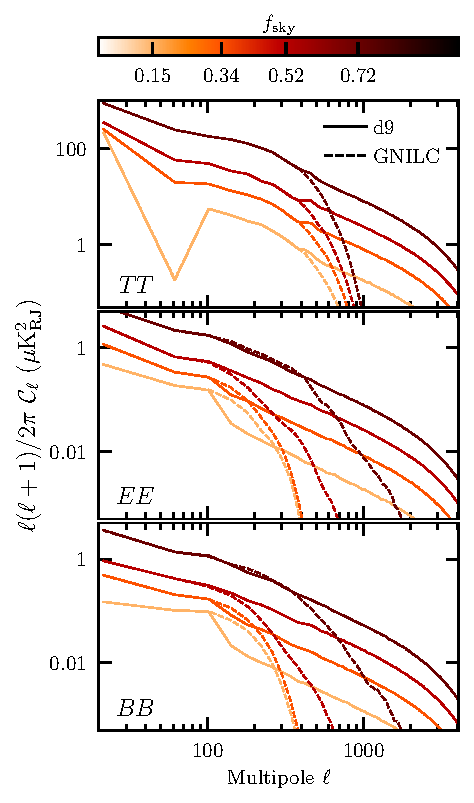
\includegraphics{paper_spectra_by_field_NSIDE2048.pdf}
%     \caption{This figure compares the power spectra of the \dnine{} model (solid lines) and the input GNILC map (dashed lines) when computed on the \texttt{GAL015}, \texttt{GAL034}, \texttt{GAL052}, and \texttt{GAL072} Galactic masks.}
%     \label{fig:spectra_by_field}
% \end{figure}

% \begin{figure}
%     \centering
%     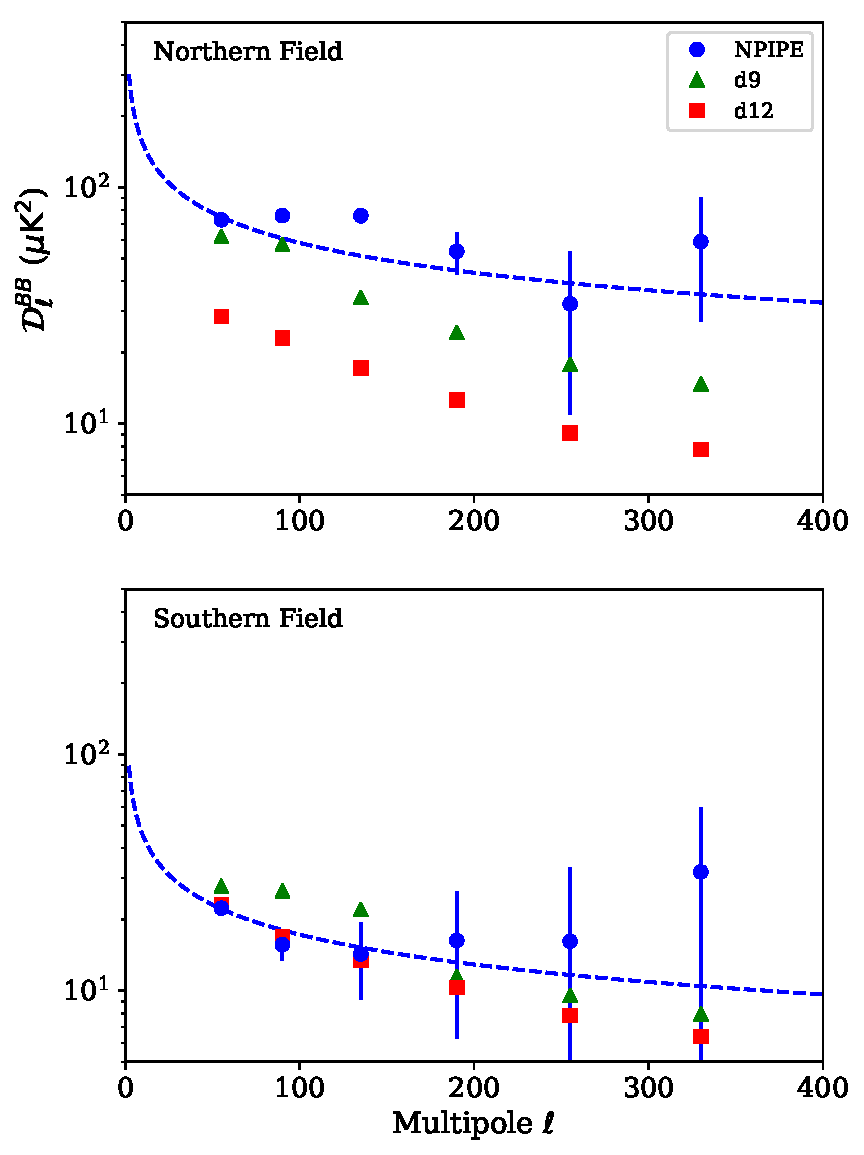
\includegraphics[width=0.48\textwidth]{figures/smallfield_power.pdf}
%     \caption{The binned $BB$ power spectra from the 353~GHz NPIPE half-ring split maps and dust model maps \texttt{d9} and \texttt{d12}. The model maps are integrated with a 353~GHz delta bandpass and the NPIPE data maps are color-corrected (i.e. scaled by a factor of 0.92) to the same single frequency. The dashed lines indicate the best-fit of the fixed-index power law ($\mathcal{D}_\ell^{BB} = A^{BB} \big( l/80 \big)^{\alpha^{BB}+2}$ where $\alpha^{BB} = -2.42$) to the NPIPE data points, which is largely driven by the first two band powers. Note that we only show the \texttt{d9} results as this model is identical to \texttt{d10} at 353~GHz.}
%     \label{fig:smallfield_power}
% \end{figure}

% \subsubsection{Small Field Power Analysis} 

% \textbf{Kenny:} To compare the small-scale performances of the latest PySM dust models \texttt{d9}, \texttt{d10} and \texttt{d12} with real data, we mainly follow the analysis method described in \cite{planck2014-XXX} to examine the model behaviors. We first use a HEALPix grid with $\texttt{nside} = 8$ to divide the full sky into 768 patches. At the center of each patch, we create a 400-square-degree circular mask with its edge tapered by a $2^\circ$ FWHM Gaussian (resulting in $f_{\rm sky} \approx 0.008$), and apply such a mask to the mean-subtracted dust model and NPIPE half-ring split maps at 353~GHz. We then use \texttt{anafast} to compute the binned $BB$ auto-spectra of the masked model maps at $\ell = 55,90,135,190,255,330$ with $\Delta \ell = 30$, and scale them to be the full-sky $\mathcal{D}_\ell^{BB}$ by dividing the apodization mask integral squared. For the masked NPIPE data maps, we instead compute cross-spectrum from the two split maps to minimize the noise correlation. The representative results from two selected circular fields at $|b| > 30^\circ$ of the northern and southern Galactic hemispheres are shown in Fig.~\ref{fig:smallfield_power}. (\textbf{Kenny:} this analysis uses anafast - contradicts with the NaMaster stated above?)

% We would like to explore whether the PySM models can reproduce the dust $BB$ power spectrum's amplitude and steepness over $\ell$ in reality, especially in those high Galactic latitude small fields. We therefore compute the low-$\ell$ averaged $\mathcal{D}_\ell^{BB}$ (over $\ell = 55, 90$) and the high-$\ell$ averaged $\mathcal{D}_\ell^{BB}$ (over $\ell = 135, 190, 255, 330$) of each small field for the model and NPIPE maps, and we present the results in scatter plots in Fig.~\ref{fig:smallfield_power_all}. It turns out that the amplitude of the \texttt{d12} model is in general smaller than the preference of NPIPE data, as a large fraction of the d12 data points cluster around the lower-left corner of the plot. The wider span of the \texttt{d12} data points along the vertical direction also implies the model spectrum steepness varies more over the sky. In contrast, the \texttt{d9}/\texttt{d10} data points are fairly compatible with the NPIPE results, although they predict slightly steeper power spectra. If we define the ratio of the low-$\ell$ mean value to the high-$\ell$ mean value as a proxy for describing the spatial power change across the modulation scale, while the perfect fixed-index power law $\mathcal{D}_\ell^{BB} \propto \ell^{-0.42}$ yields a value of $\approx 1.60$, the NPIPE maps give $1.65 \pm 0.68$ and the \texttt{d9}/\texttt{d10} (\texttt{d12}) model map gives $2.37 \pm 0.77$ ($2.24 \pm 0.87$) over sky patches with $|b| > 30^\circ$.

% \begin{figure}
%     \centering
%     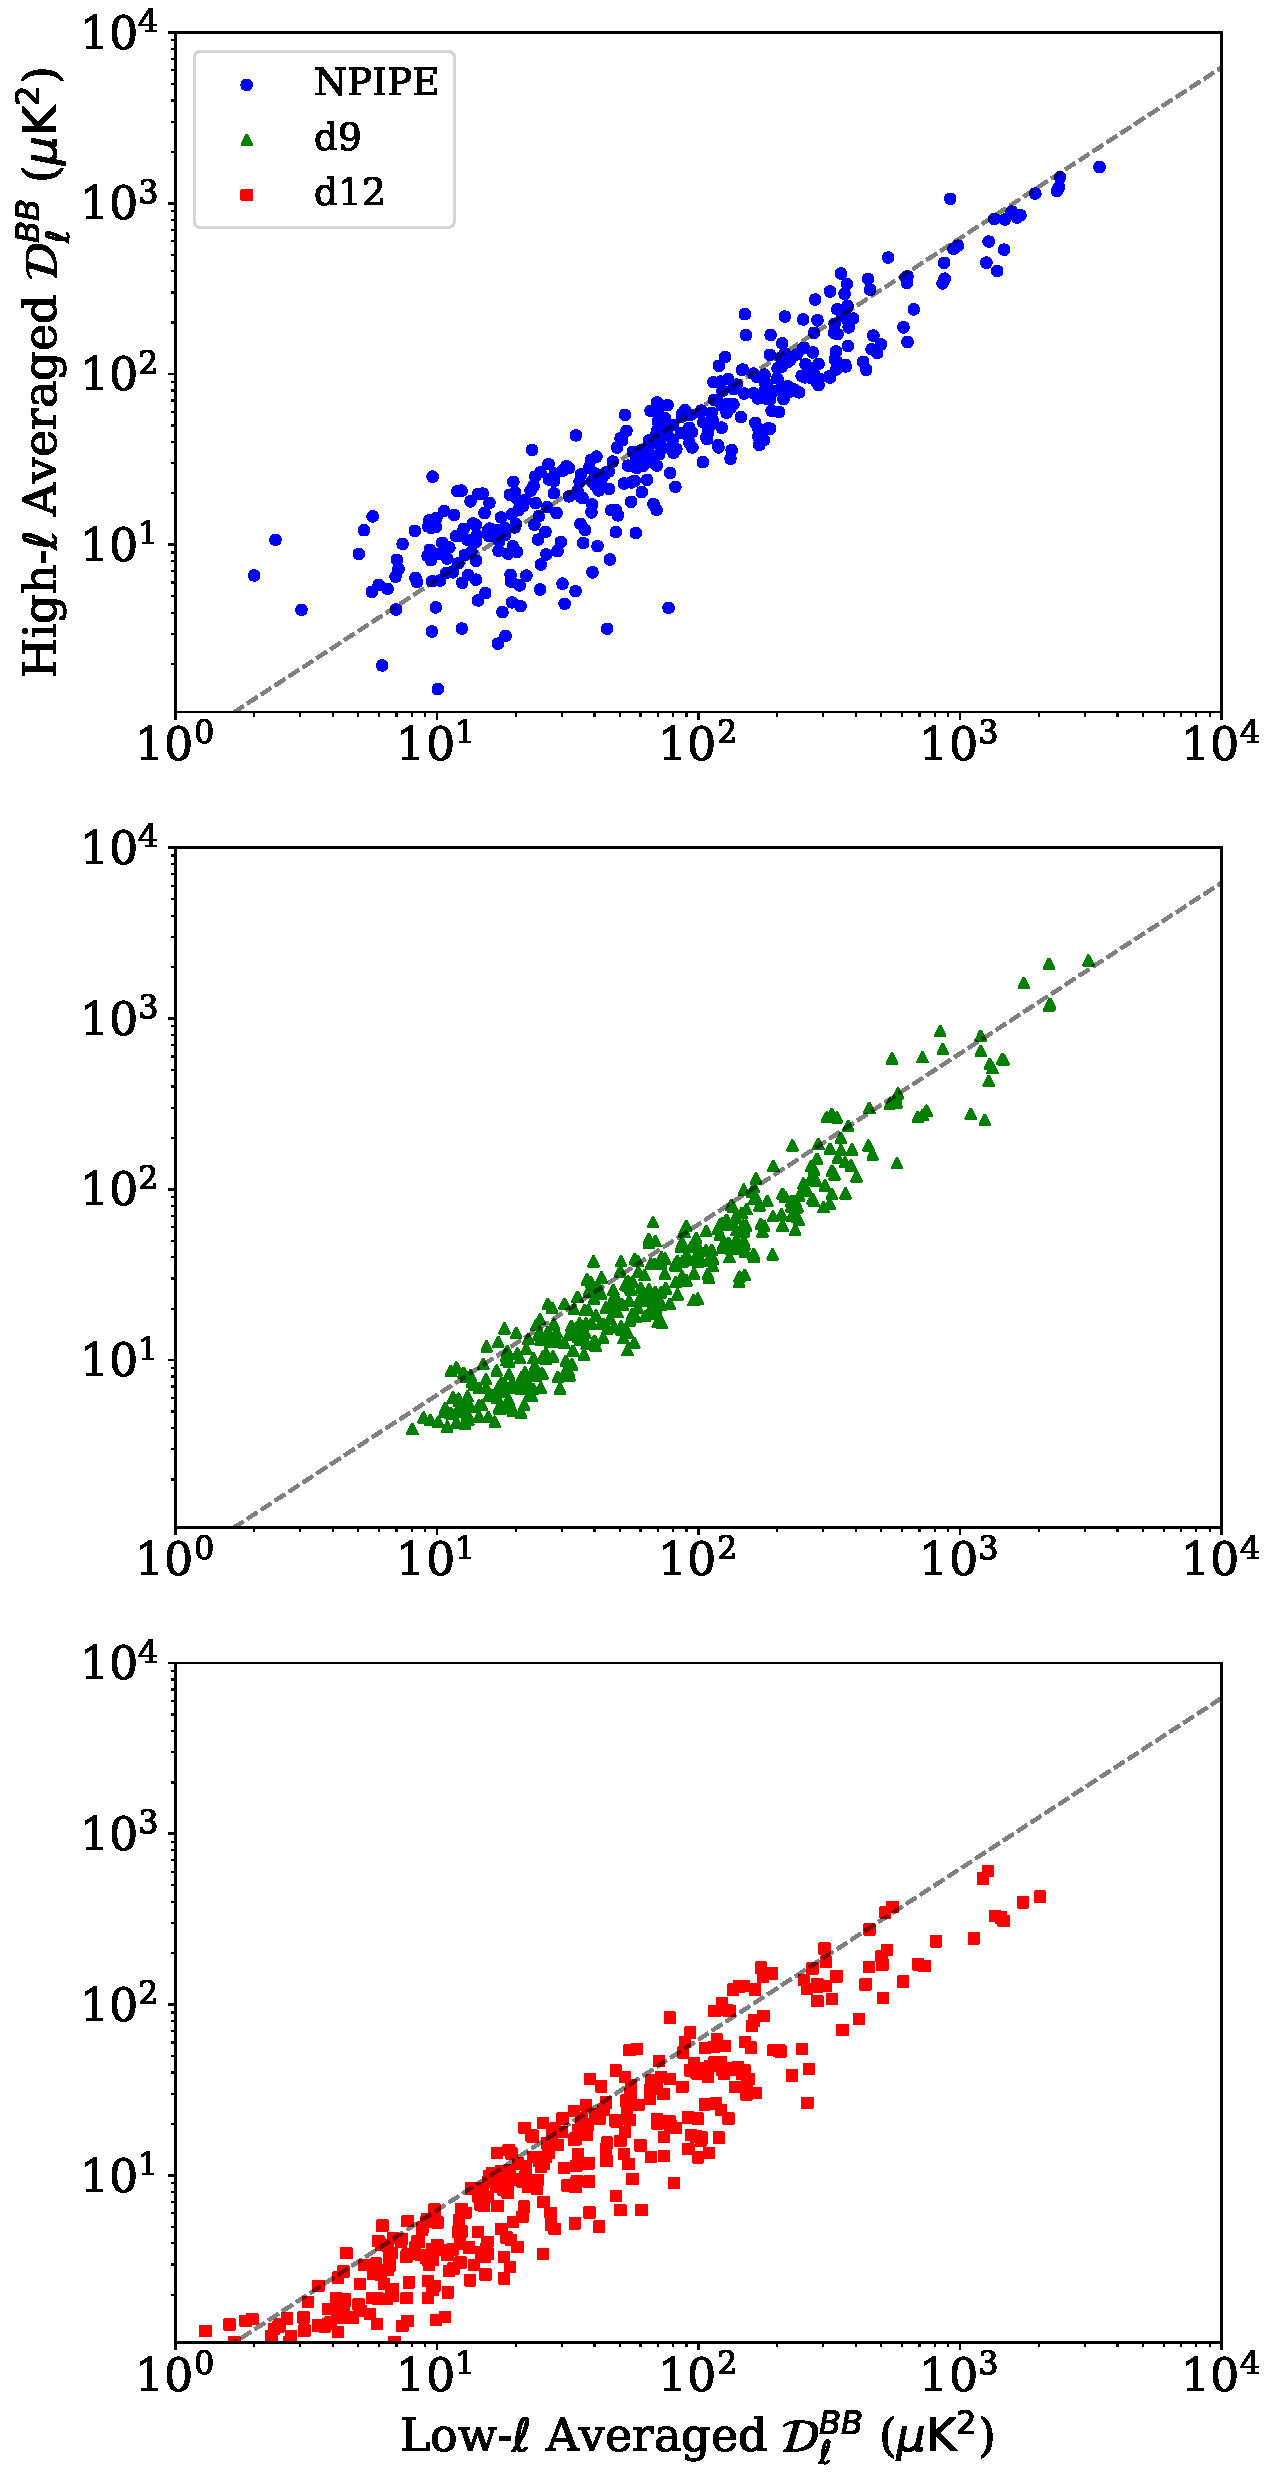
\includegraphics[width=0.48\textwidth]{figures/all2_lhmean.pdf}
%     \caption{Scatter plots of the mean of the first two $BB$ band powers versus the mean of the last four $BB$ band powers shown in Fig.~\ref{fig:smallfield_power}. Each data point represents the results from a circular sky patches with $|b| > 30^\circ$. Dashed reference lines indicating $\mathcal{D}_\ell^{BB} \propto \ell^{-0.42}$ are added to the plots. This power law in fact comes from the analysis of several larger sky regions ($f_\text{sky} = 0.3 \; \text{to} \; 0.8$) by \cite{planck2014-XXX}, but the small-field NPIPE data points, which spread out when the dust amplitude is small presumably due to map noise, are consistent with it as well. Another important feature is that the trends of the \texttt{d9} and \texttt{d12} data points are lower than that of the NPIPE in these log-log plots, implying that the model spectra are steeper.}
%     \label{fig:smallfield_power_all}
% \end{figure}

% \subsubsection{BICEP / Keck} \label{sec:bkspt_spectra}

% \textbf{Ben:} The current upper limit on the tensor-to-scalar ratio is set by a combination of BICEP / Keck (BK), Planck, and WMAP data: $r < 0.036~(95\%)$ \citep{Ade:2021}. Over the next few years, a collaborative effort between the South Pole Telescope (SPT) and BICEP / Keck will combine high-resolution SPT-3G observations with BK observations in order to ``delens'' the observed CMB B-modes, and further constrain $r$. Therefore, there will be continued interest in simulating Galactic foregrounds on this particular patch of sky.

% In Figure~\ref{fig:d1d9_bkpatch} we compare the BB power spectrum of the new \dnine{} model with the original PySM \done{} model, the GNILC input map, and the maximum likelihood dust model in this patch of sky determined from a combination of BK, Planck and WMAP data \citep{Ade:2021}. Model \done{} clearly has excess dust BB power compared to the measured amplitude in this patch of sky, which has been known for some time. This is somewhat ameliorated in model \dnine{}, primarily due to the steeper spectral tilt of the \dnine{} model leading to a factor of $\sim 10$ decrease in power relative to \done{} by multipoles of $\ell \gtrsim 300$. At larger scales of $\ell \lesssim 50$ both the \done{} and \dnine{} models are dominated by the underlying GNILC template, rather than the simulated small scale realizations, and so the mismatch in amplitude between the BK maximum likelihood model and our templates is most likely due to residual noise in the GNILC template. Indeed, most of the constraining power on dust BB power in Ref~\cite{Ade:2021} is driven by BK observations at 220\,GHz, which are not used to inform our model. 

% One may argue that the amplitude and spectral tilt of the \dnine{} model clearly disagree with existing observations in the BK patch of sky. While this is true, it is beyond the scope of this work to provide full sky simulations that guarantee consistency with all sets of full sky and partial sky observations. Indeed, the use of power spectrum-based techniques requires a certain amount of global averaging of power spectrum parameters that are in fact known to vary across the sky \cite{planck2016-l04}. For example, while the dust amplitude can be modulated by the use of a large scale template, the spectral tilt has to be fixed to a single value for the full sky, which is not realistic. 

% \begin{figure}[ht]
%     \centering
%     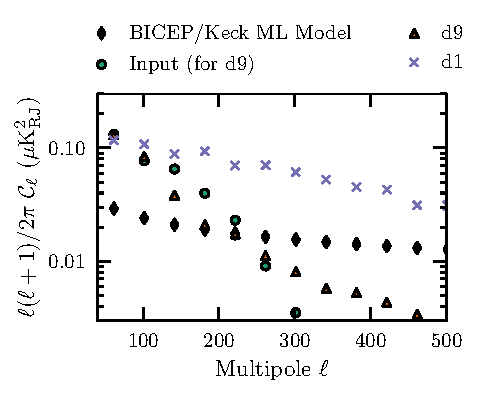
\includegraphics{paper_BK_patch.pdf}
%     \caption{This figure shows the BB power spectra of the \done{} (crosses), \dnine{} (triangles), and varres GNILC map (circles), compared to the maximum likelihood BK dust model (black diamonds) derived from a combination of WMAP and Planck with BICEP / Keck data up to the 2018 observing season. Note that in order to make a meaningful comparison between the bandpowers calculated from maps and the theory curve, we first convolve the theory spectrum with the mode-coupling matrix and then compute the decoupled bandpowers by applying the inverted binned coupling matrix.}
%     \label{fig:d1d9_bkpatch}
% \end{figure}

% \subsubsection{Map level validation}
% %In this section, we present a map-level validation of the PySM dust models \dnine{}, {\tt d11}, {\tt d12} models against the Planck third data release (PR3) \cite{}.
% \textbf{Elisa}: In this section, we compare at the map level, Planck third data release PR3 \cite{planck2016-l03}) and PySM dust models \dnine{}, {\tt d11}, {\tt d12} models. We study how well the modeled intensity $I$ and polarized intensity $P = \sqrt{U^2 + Q^2}$ match the observations on three selected $16.7^\circ \times 16.7^\circ$ patches of the sky, at 353~GHz. Here, we focus on two local patches: close to the Galactic plane ($[l,b] =[180^\circ,-10^\circ]$) and, centered on the Bicep / Keck field ($[l,b] =[318^\circ,-61^\circ]$).
% Similar to Section~\ref{sec:sync_validation}, we integrate the dust models within the Planck passbands to enable direct comparison. For comparison of intensity maps, we subtract a Wiener-filtered CMB temperature anisotropies map from SMICA and adjust the zero level of the PR3 data to that of the simulated map over regions of faint dust intensity on the sky.
% The mask used to adjust the zero levels is shown in figure \ref{fig:mask_zero_lvl_int}. These corrections are not required for comparing polarization data.
% \begin{figure}[ht!]
%     \centering
%     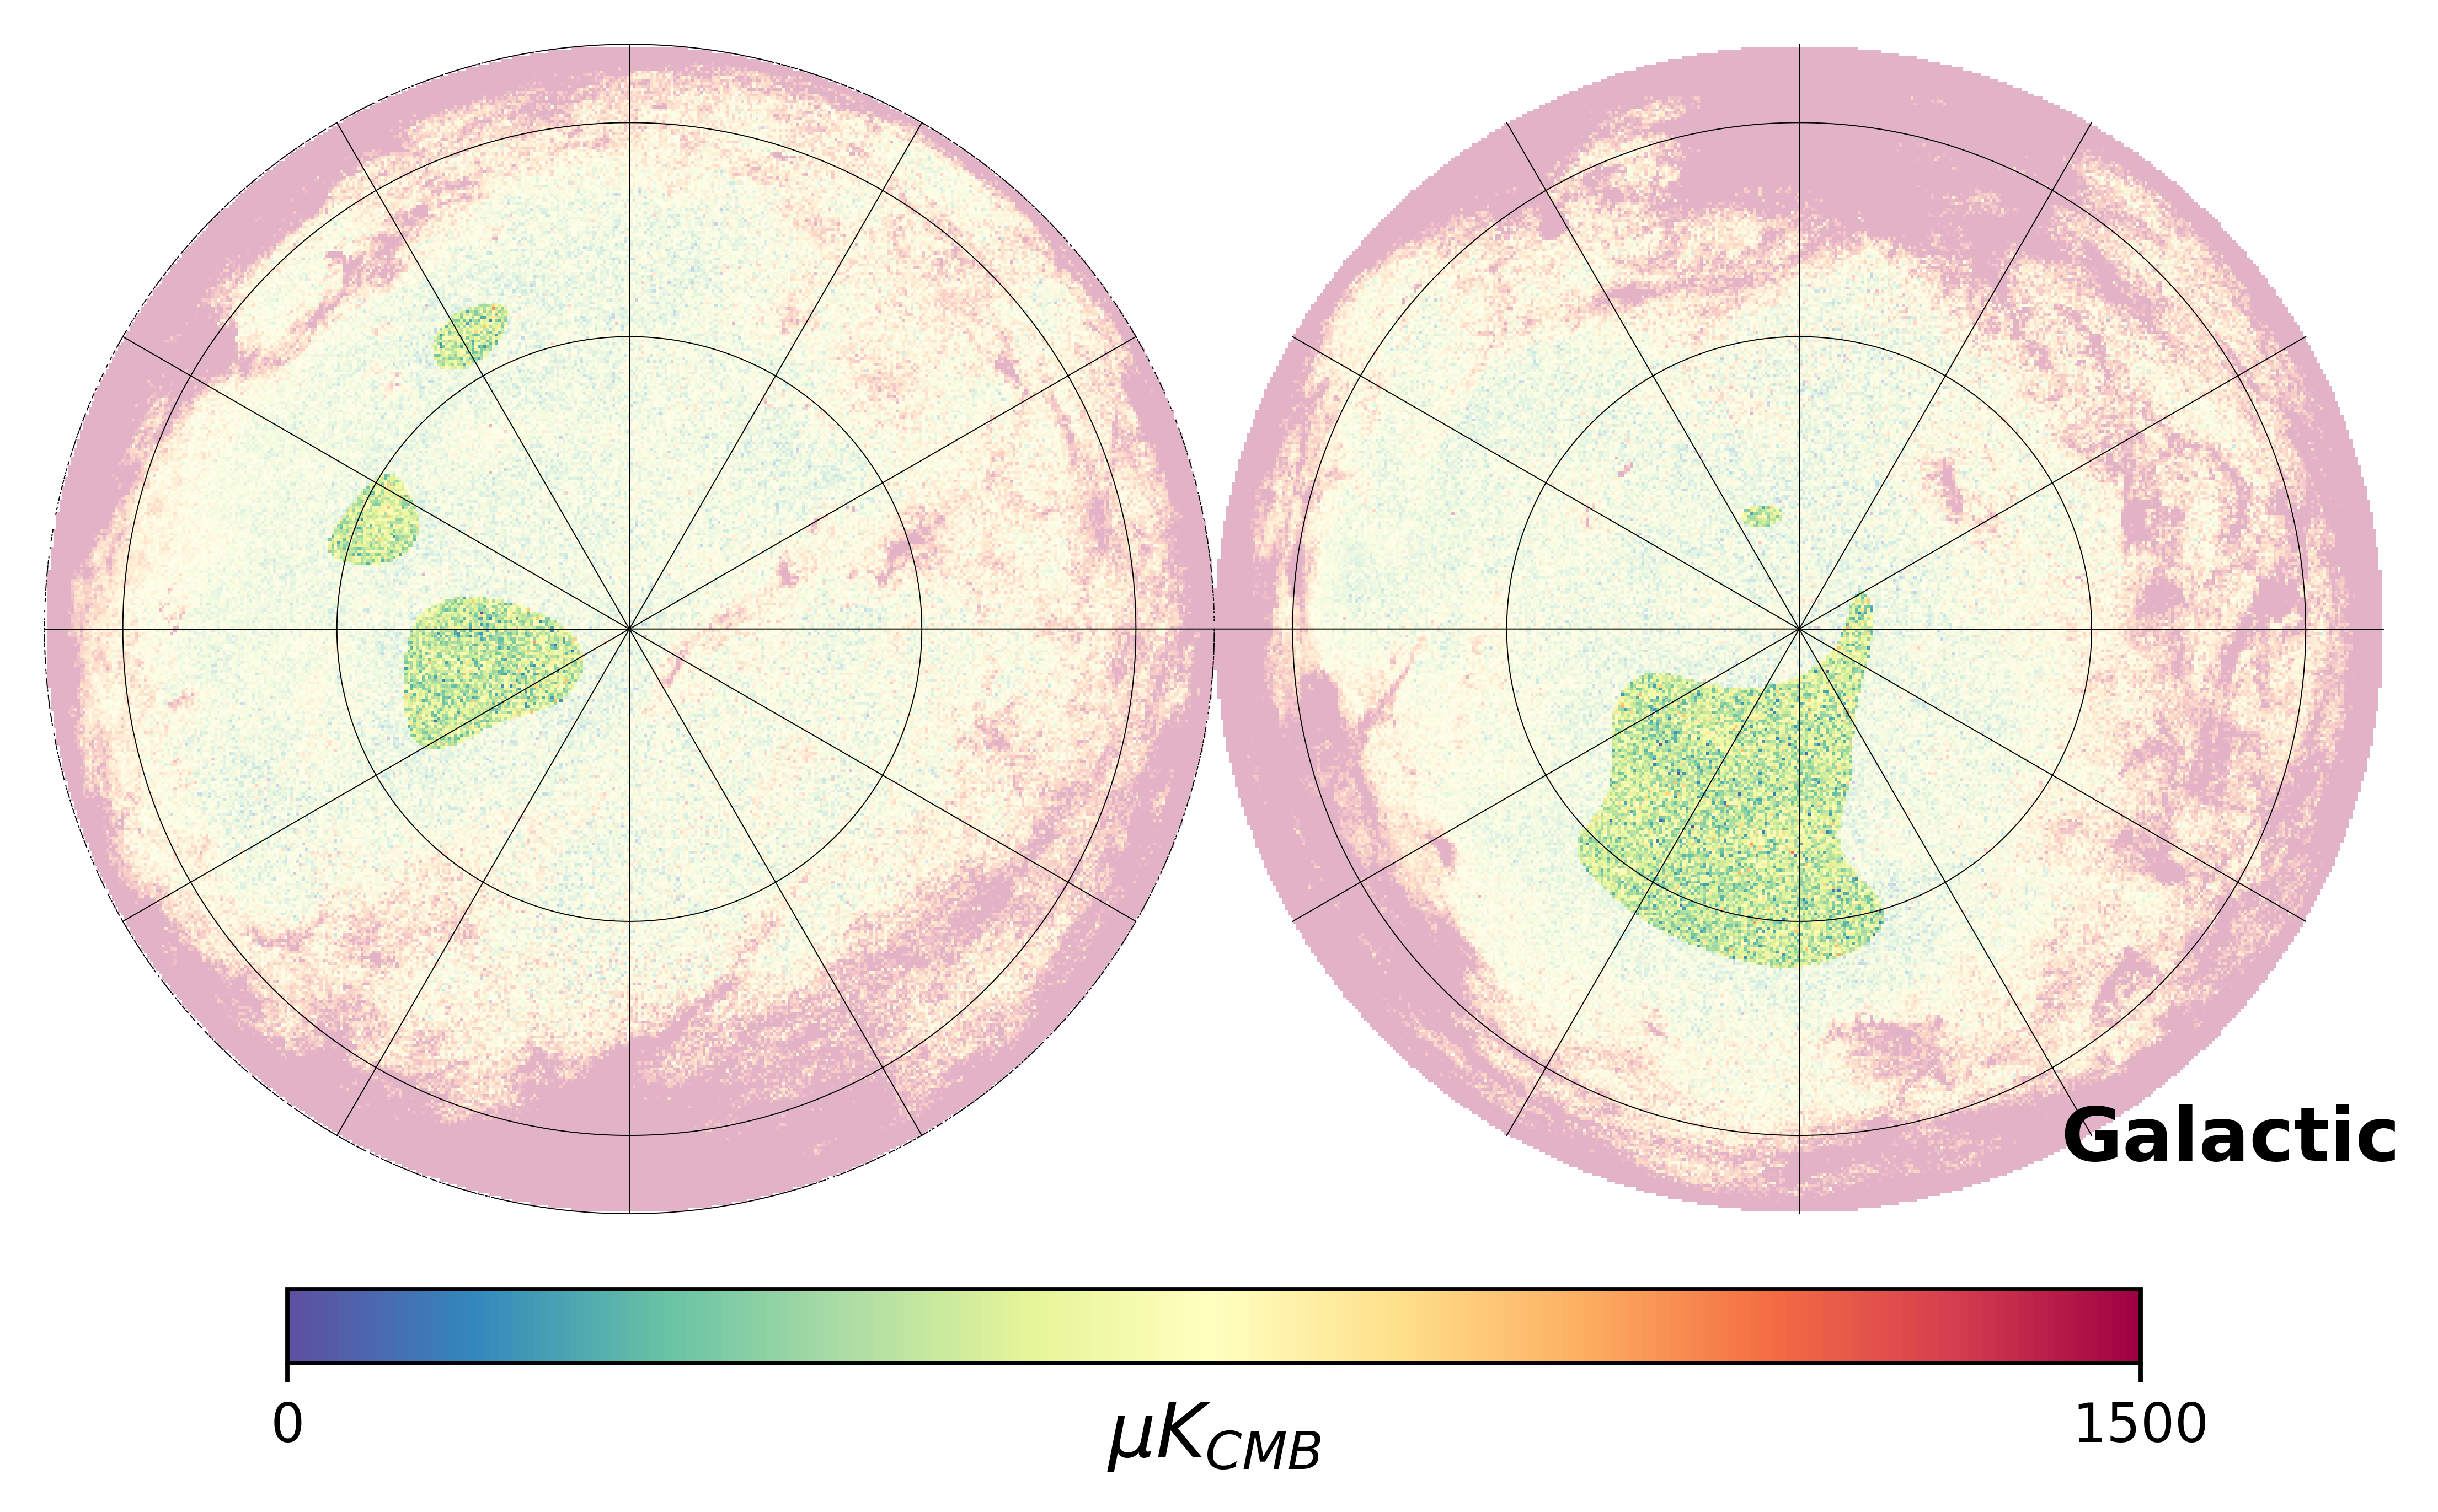
\includegraphics[width=0.48\textwidth]{figures/mask_intxPR3_zero_lvl.png}
%     \caption{Mask $\times$ PR3 intensity used to estimate the zero level of PR3 intensity. This mask is obtained by thresholding the intensity of the smoothed PR3 intensity to preserve only the regions where the dust is very low, to estimate the zero-level of the data and models.}%more details
%     \label{fig:mask_zero_lvl_int}
% \end{figure}

% \begin{figure}[ht!]
%     \centering
%     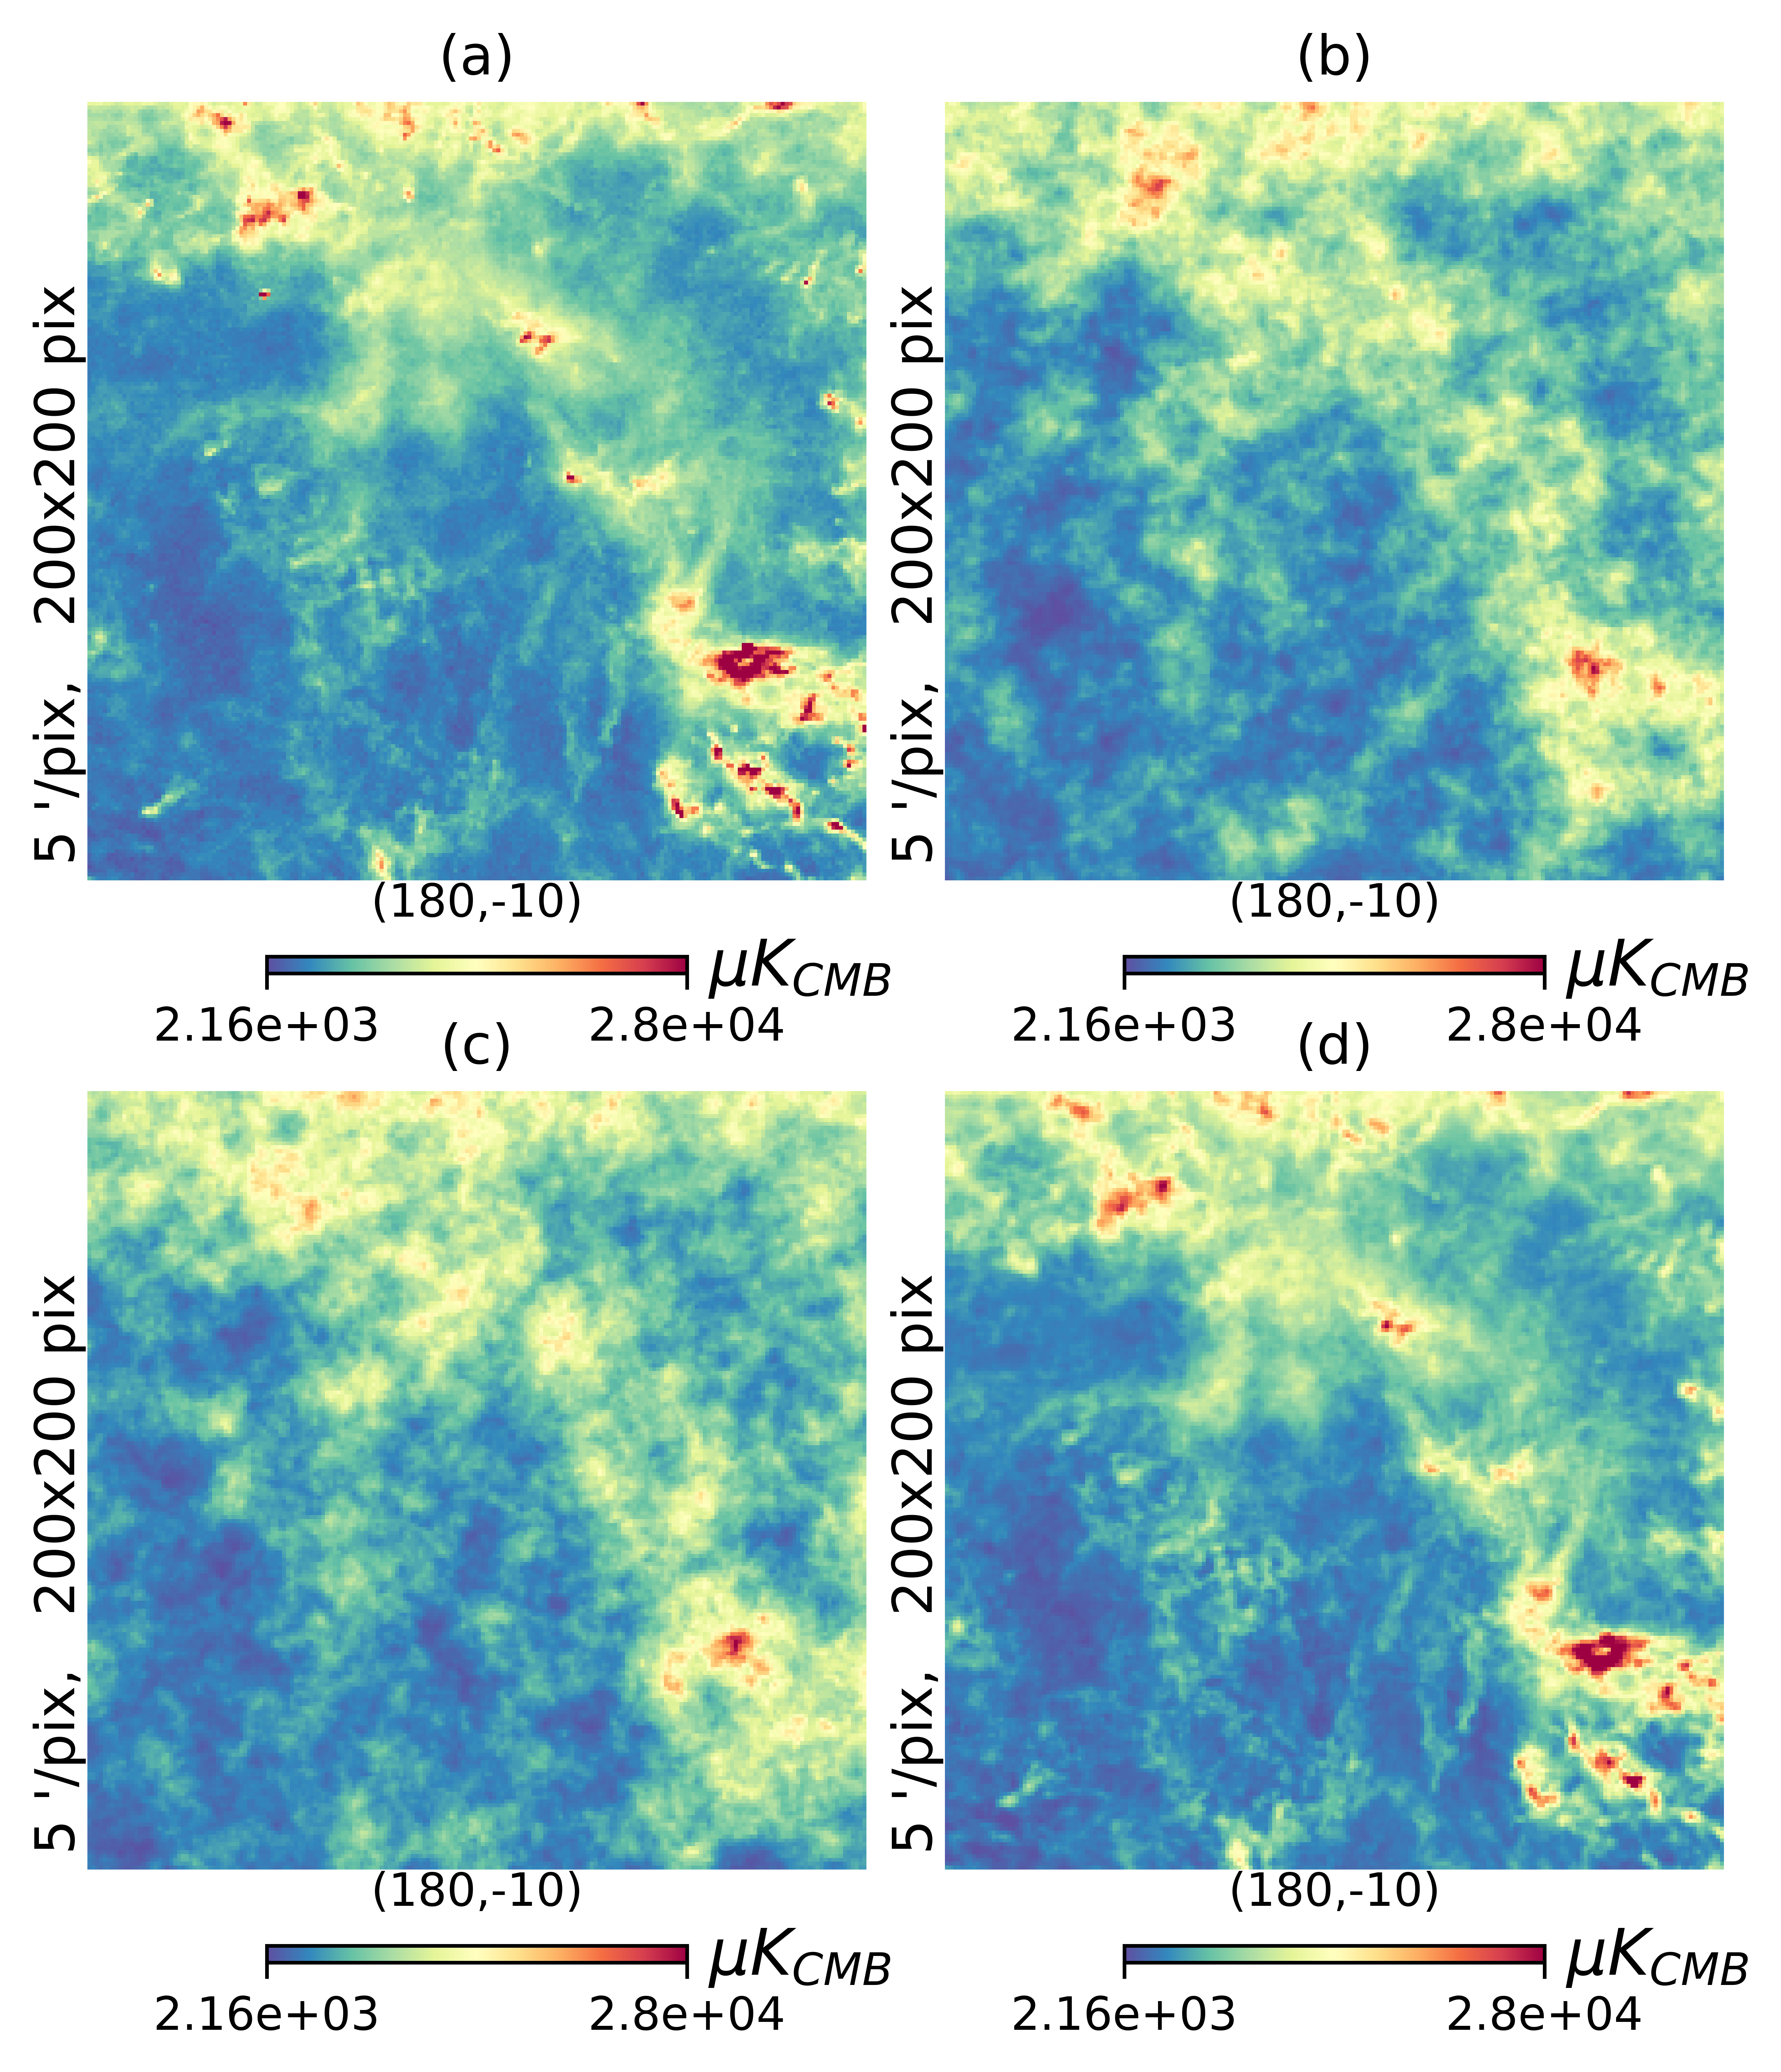
\includegraphics[width=0.48\textwidth]{figures/gal_plane_non_smooth_wo_zero_lvl.png}
% \caption{Dust intensity at 353GHz at [l = 180, b = -10] with an angular resolution of 4.94': (a) PR3 (b) d9 (c) d11 (d) d12}    
% \label{fig:353_int_gal_plane}
% \end{figure}
% % \begin{figure}
% %     \centering
% %     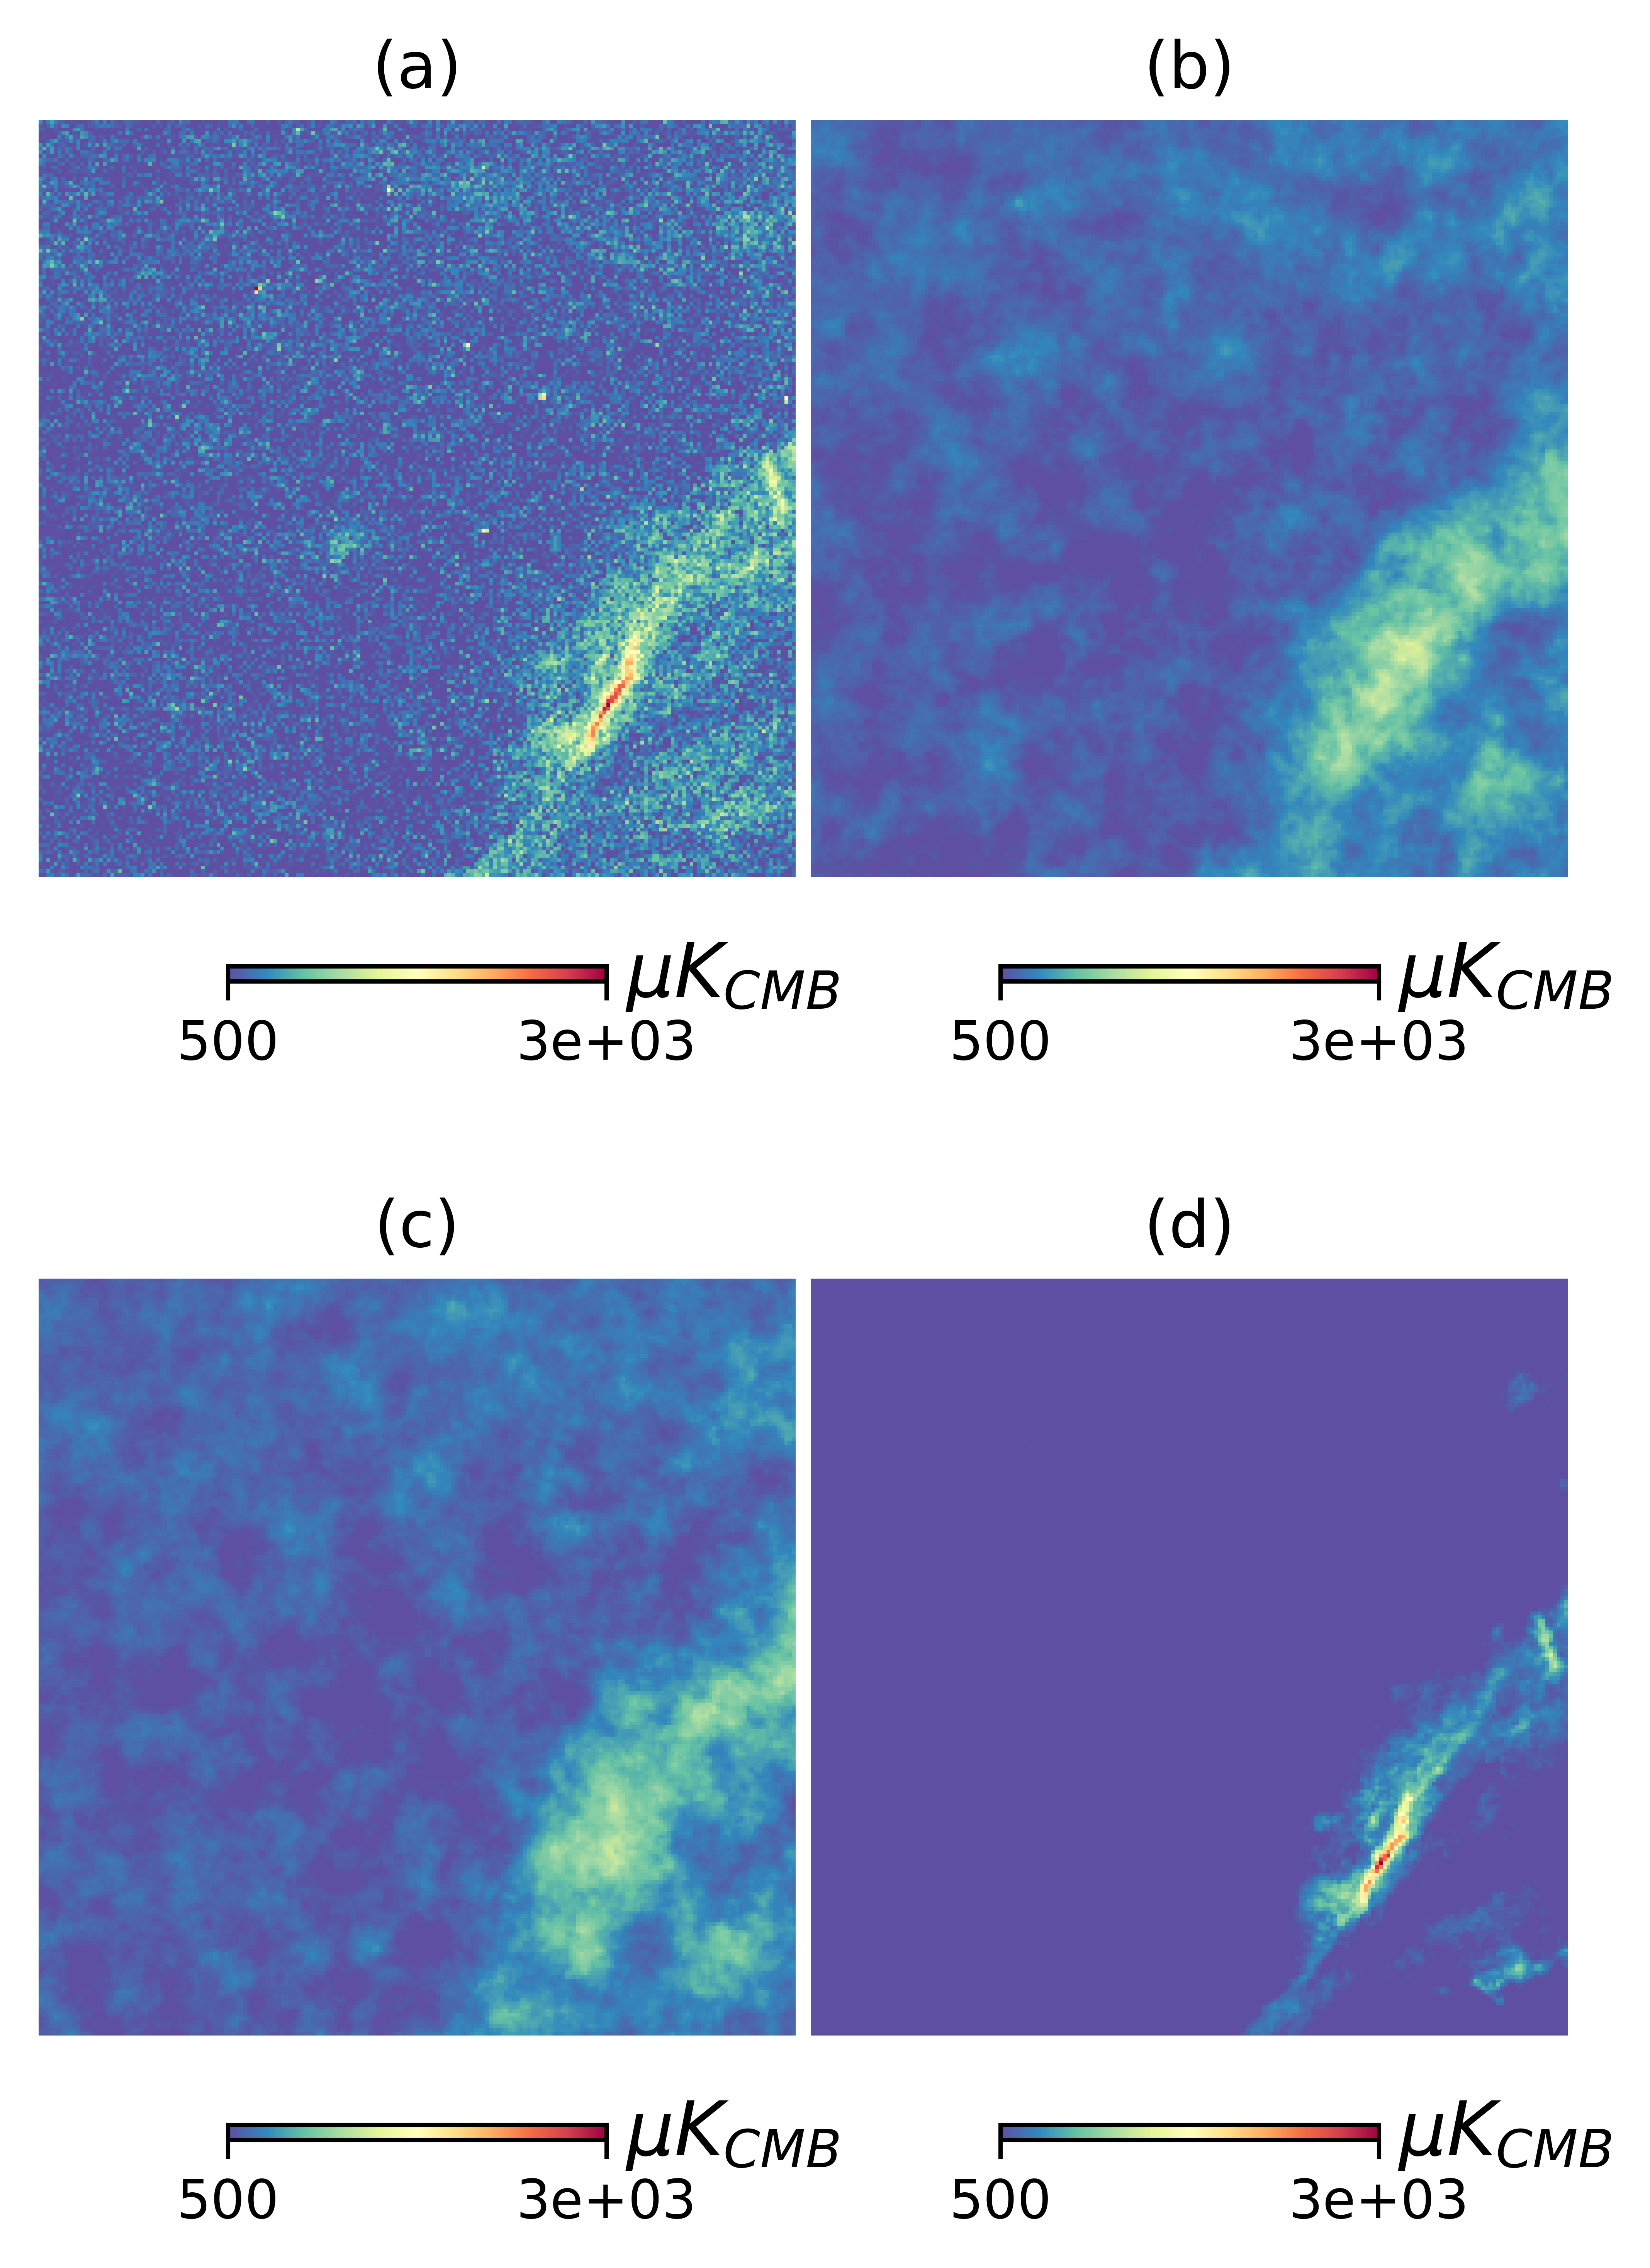
\includegraphics[scale = 0.6]{figures/NGP_non_smooth_wo_zero_lvl.png}
% %     \caption{Dust intensity at 353GHz centered at [l = 0, b = 90]: (a) PR3 (b) d9 (c) d11 (d) d12}
% %     \label{fig:353_int_NP}
% % \end{figure}
% \begin{figure}[ht!]
%     \centering
%     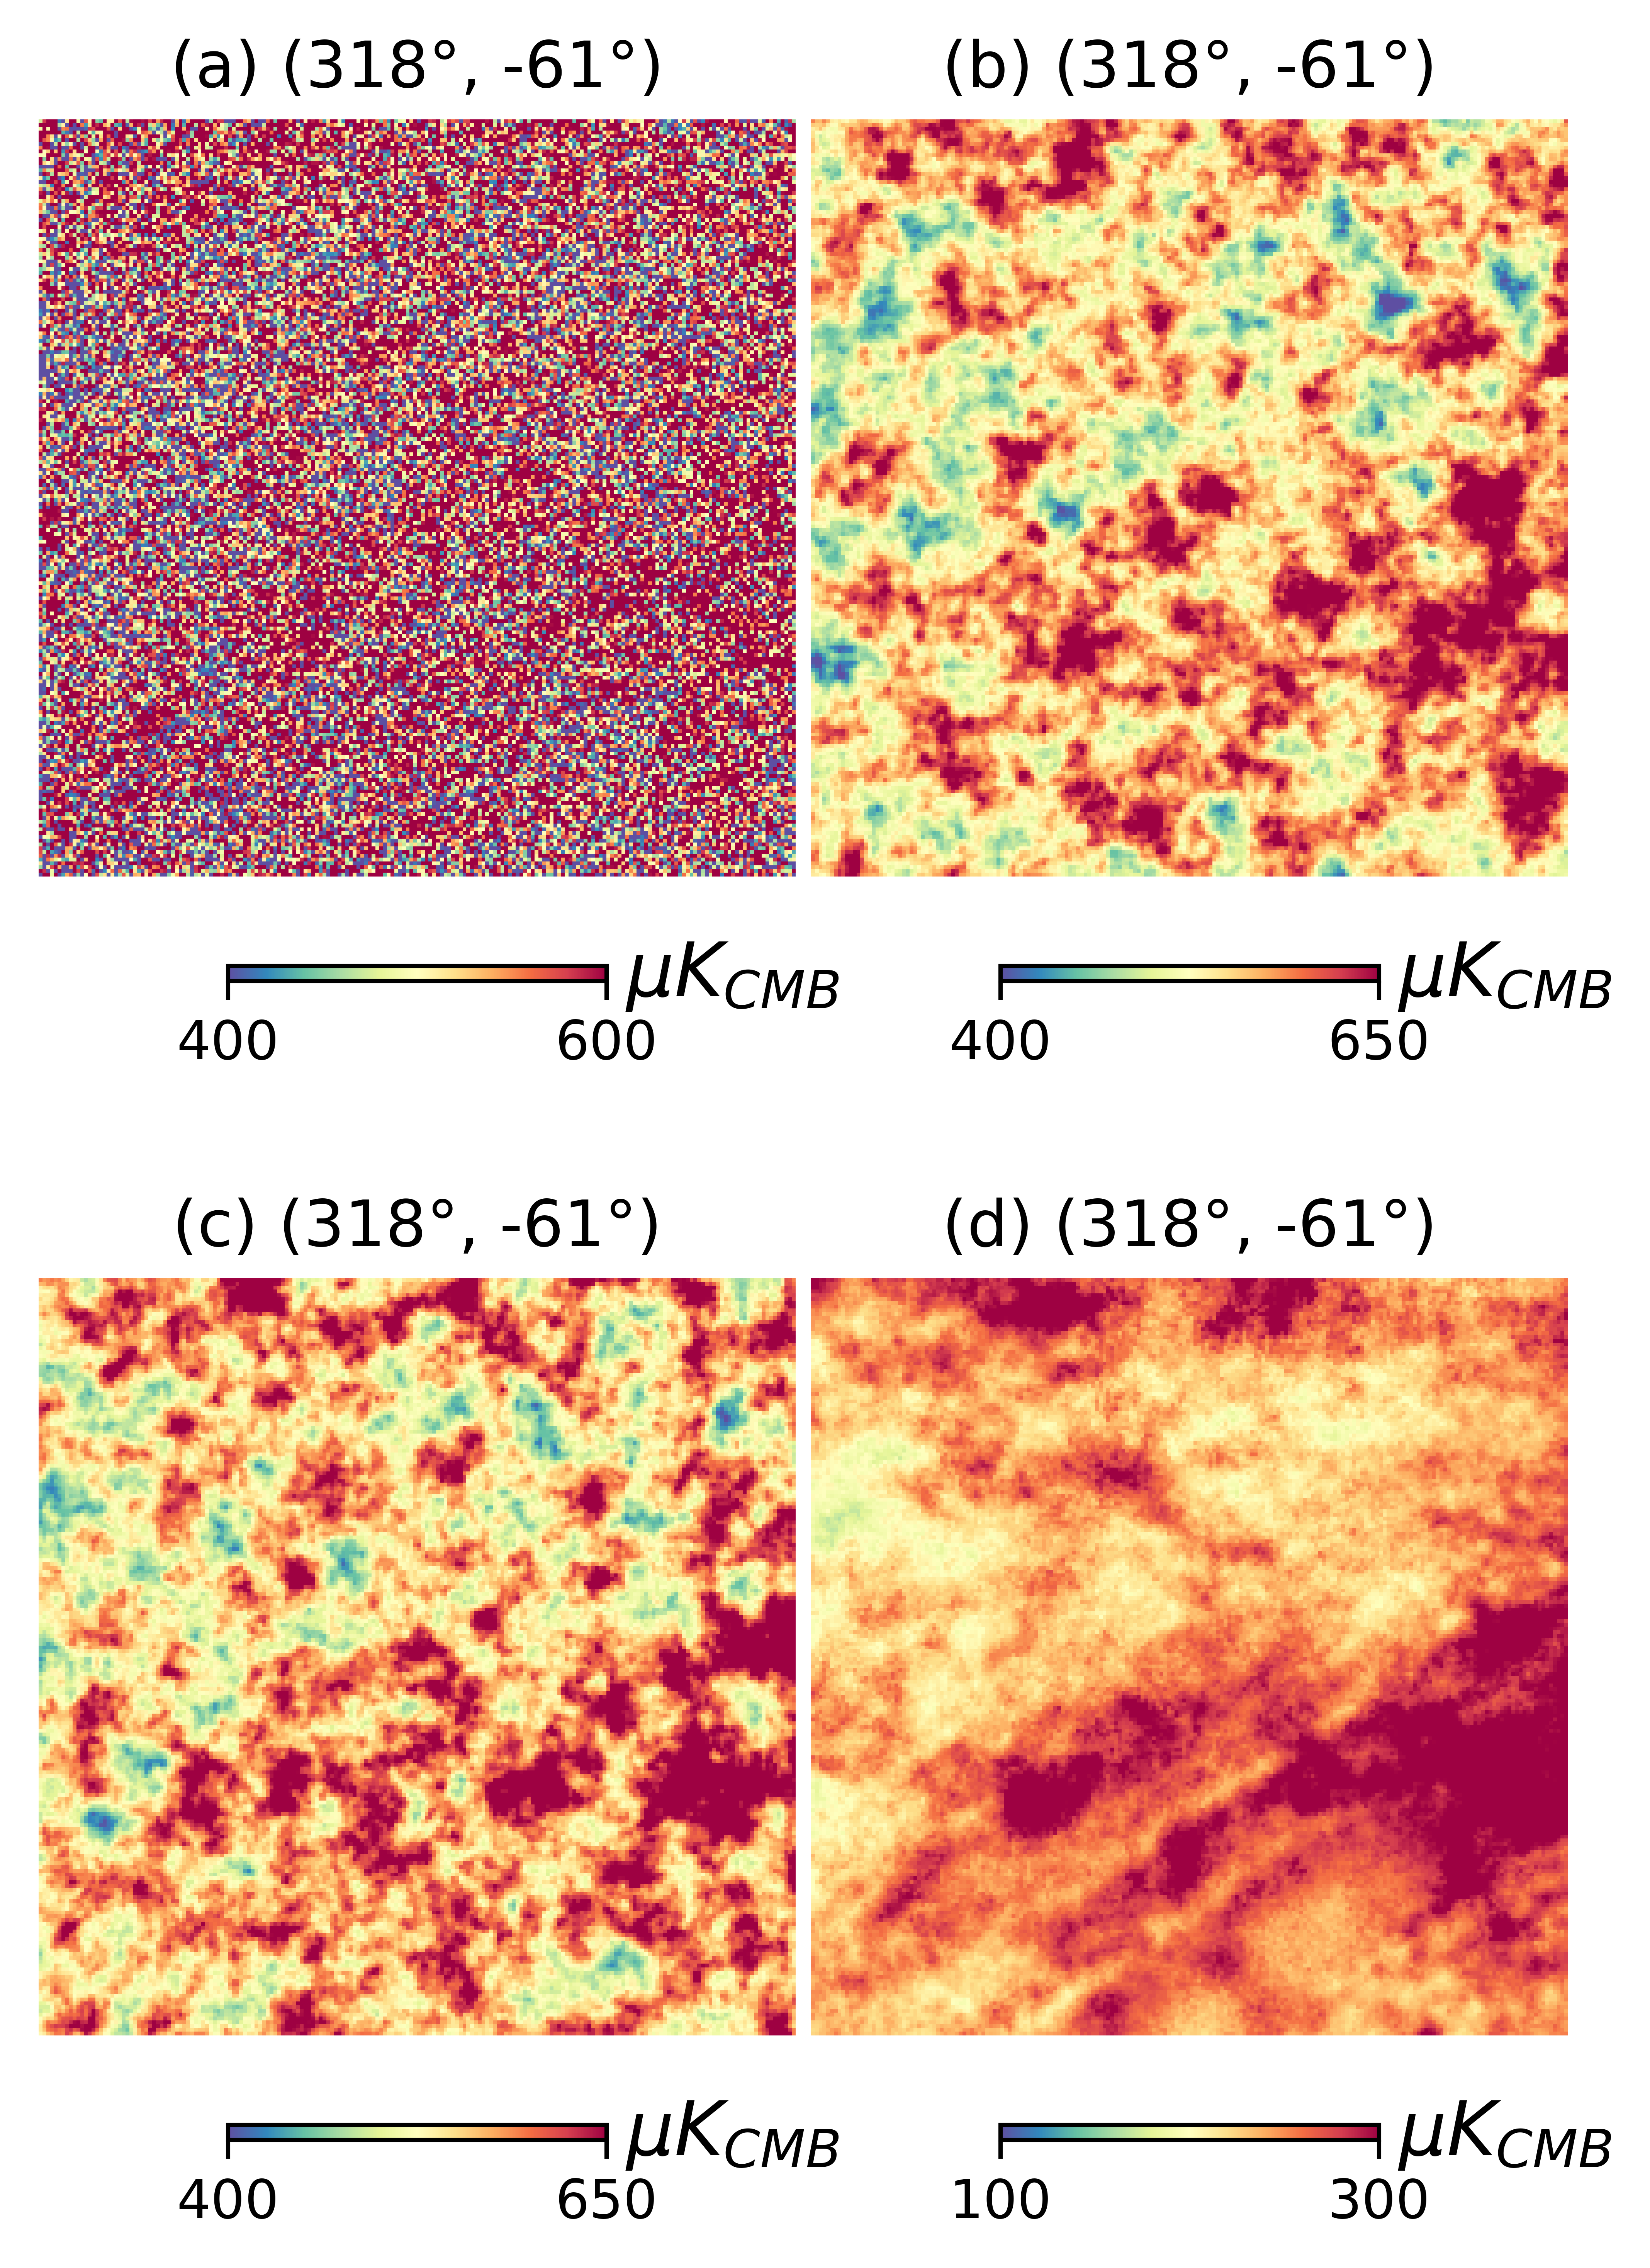
\includegraphics[width=0.48\textwidth]{figures/BK_non_smooth_wo_zero_lvl.png}
%     \caption{Dust intensity at 353GHz at [l = 318, b = -61] with an angular resolution of $4.94\arcmin$: (a) PR3 (b) d9 (c) d11 (d) d12. Here, PR3 is contaminated by CIB and extragalactic sources.}
%     \label{fig:353_int_BK}
% \end{figure}

% \begin{figure}[ht!]
%     \centering
%     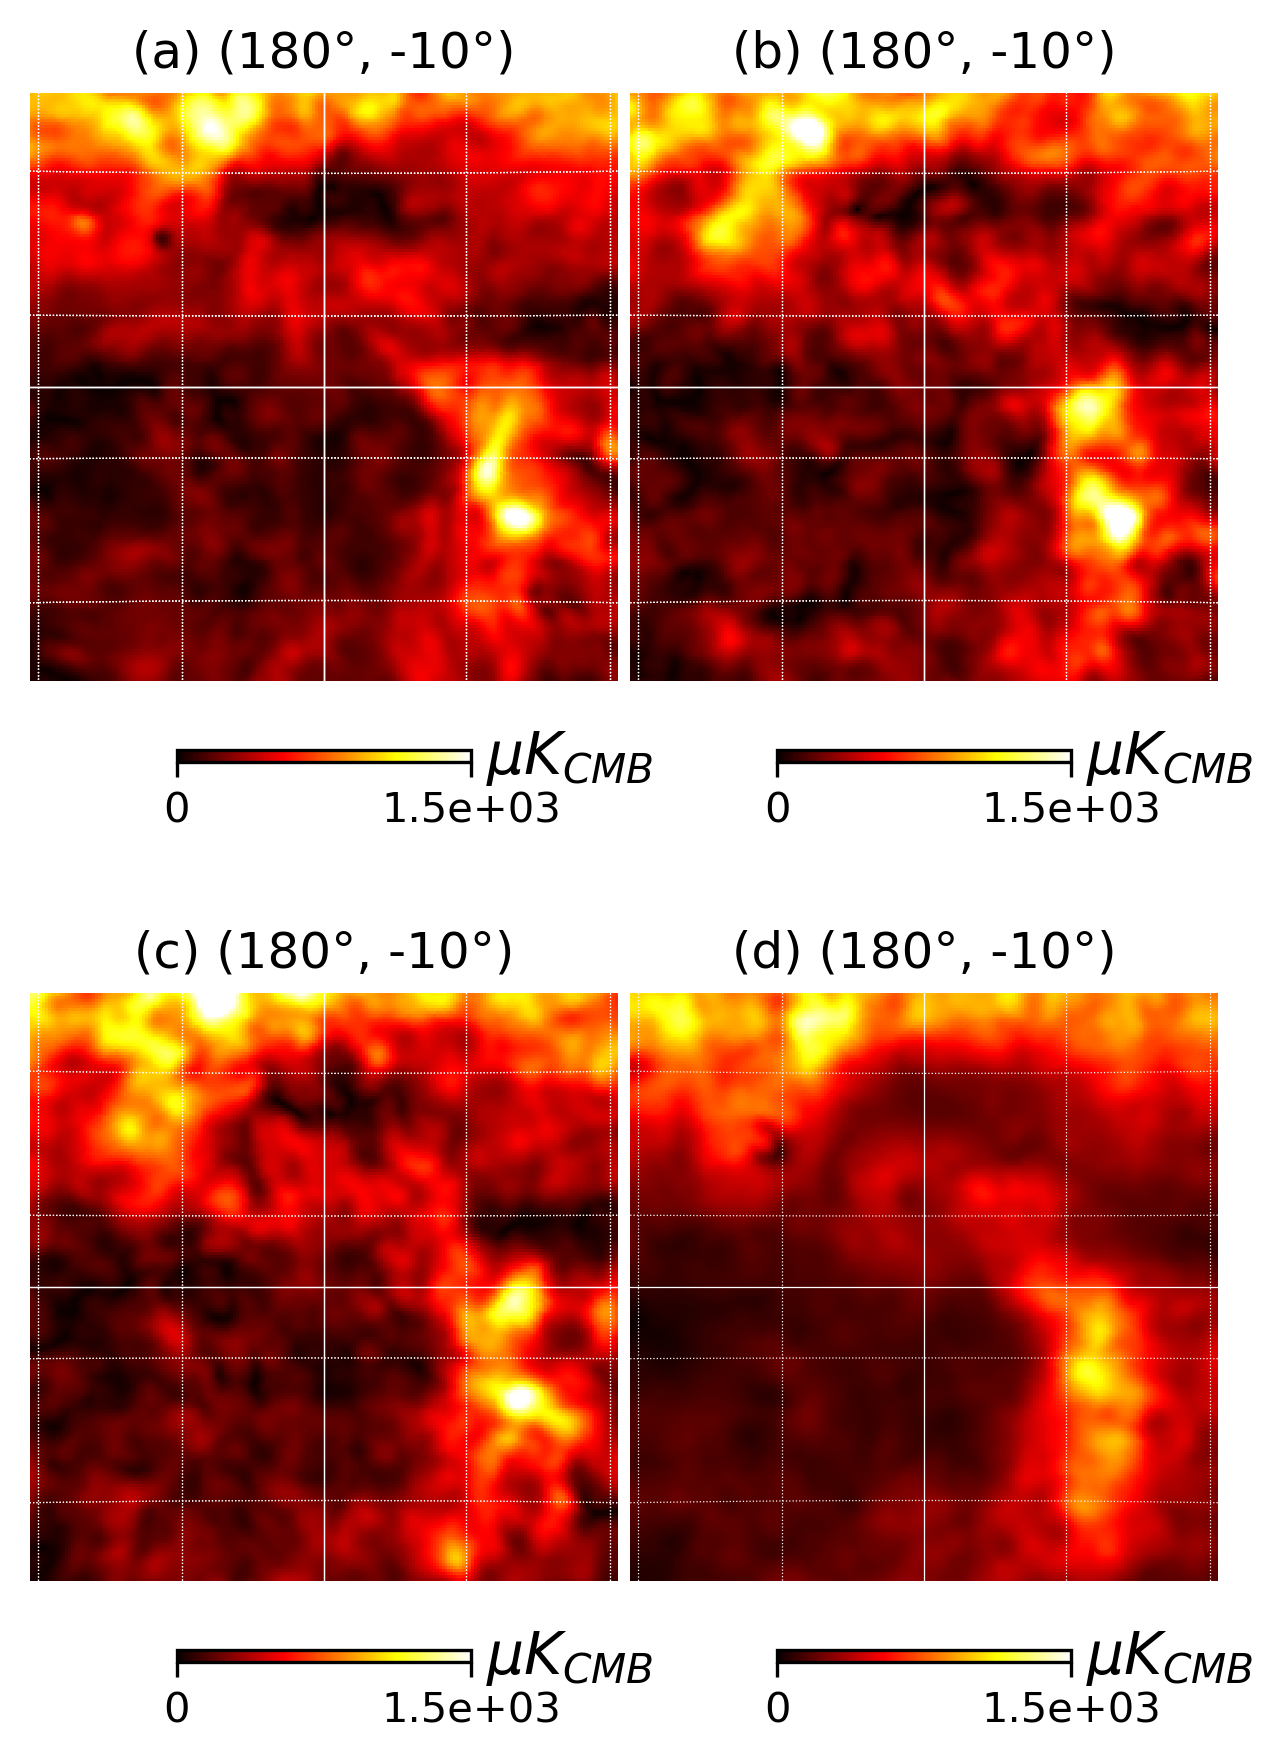
\includegraphics[width=0.48\textwidth]{figures/pol_gal_plane_smooth_30'.png}
%     \caption{Polarized dust intensity at 353GHz centered at [l = 180, b = -10] with an angular resolution of 4.94', smoothed to 30 arcmin: (a) PR3 (b) d9 (c) d11 (d) d12.}
%     \label{fig:353_pol_int_gal_plane}
% \end{figure}
% % \begin{figure}
% %     \centering
% %     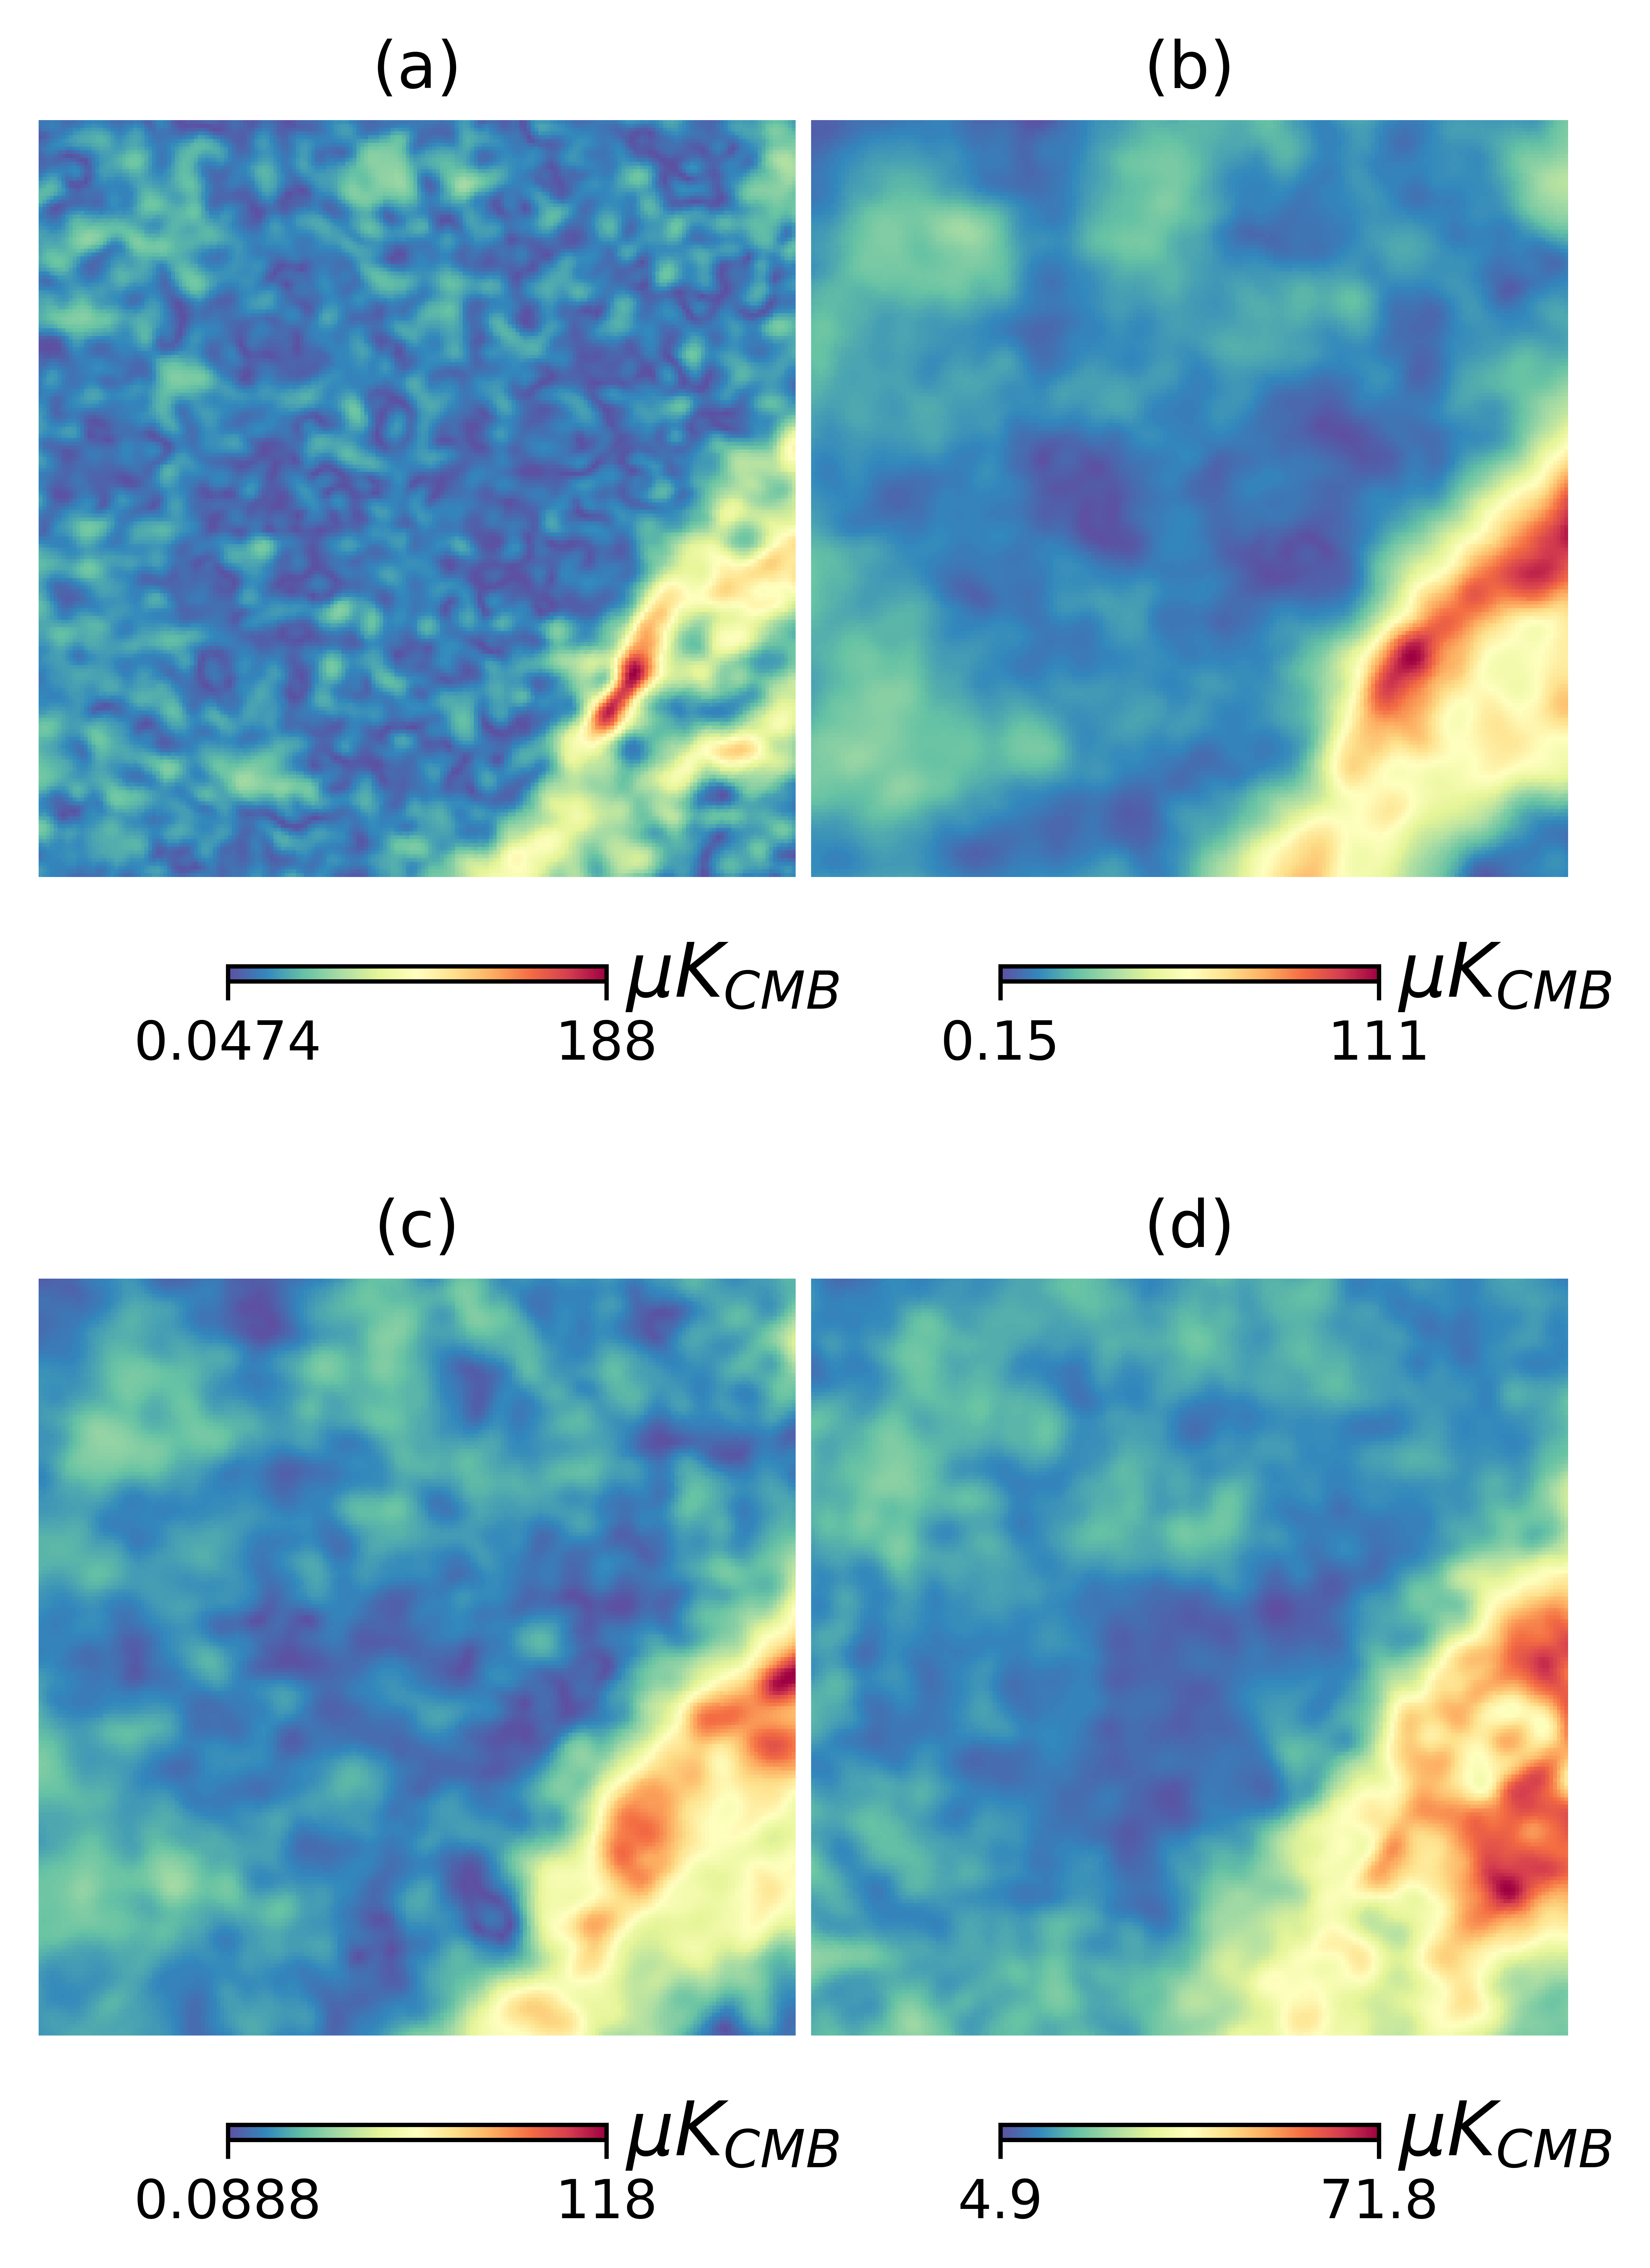
\includegraphics[scale = 0.6]{figures/pol_NGP_smooth_30'.png}
% %     \caption{Polarized dust intensity at 353GHz centered at [l = 0, b = 90].}
% %     \label{fig:353_pol_int_NGP}
% % \end{figure}

% \begin{figure}[ht!]
%     \centering
%     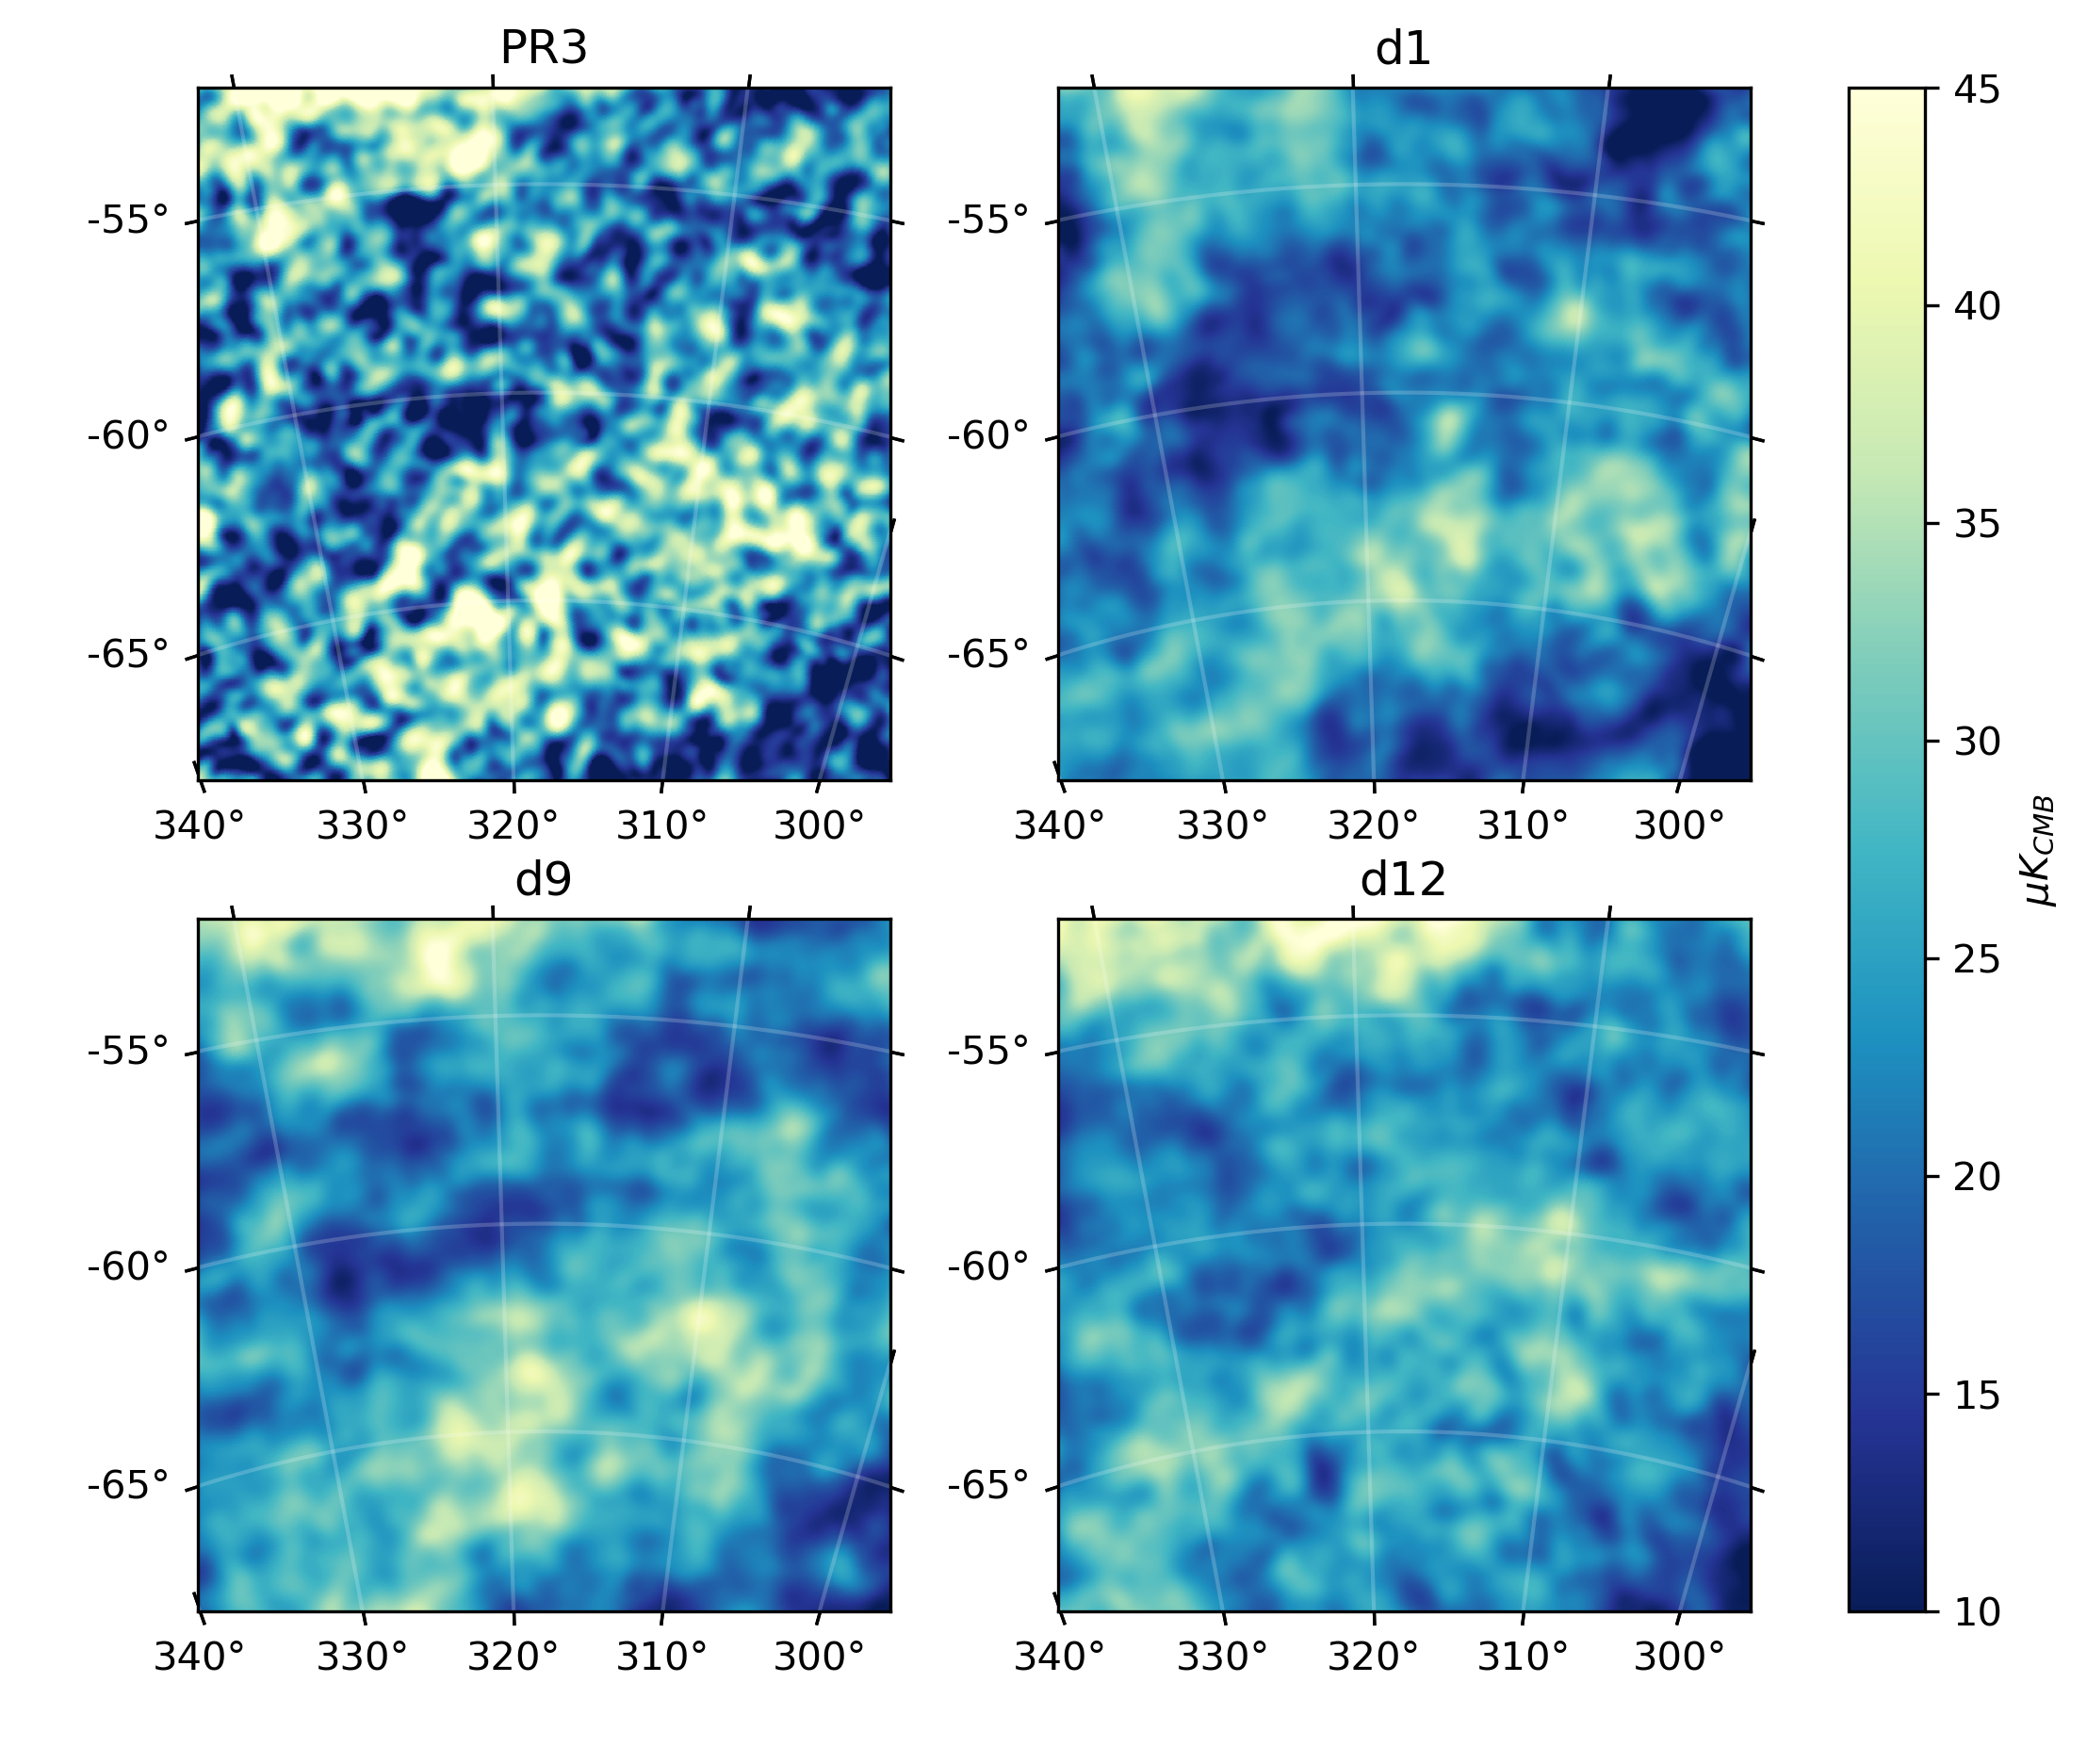
\includegraphics[width=0.48\textwidth]{figures/pol_BK_smooth_30'.png}
%     \caption{Polarized dust intensity at 353GHz centered at [l = 318, b = -61] with an angular resolution of 4.94', smoothed to 30 arcmin: (a) PR3 (b) d9 (c) d11 (d) d12.}
%     \label{fig:353_pol_int_BK}
% \end{figure}

% Intensity and polarization at 353~GHz are displayed in Figures~\ref{fig:353_int_gal_plane} to \ref{fig:353_pol_int_BK}. Varying choices for filtering the real data and generation of random small scales result in varying dust emission properties. For Intensity, d9 and d11 are very similar, with a loss of real structures, replaced by random realizations up to a scale of $l_{max} = 16384$, while d12 is more similar to the actual data. 
% Around the Bicep / Keck patch center (Figure~\ref{fig:353_int_BK}), the PR3 data is contaminated by the CIB, which masks out dust emission. 

% For the polarized intensity, close to the Galactic plane (Figure \ref{fig:353_pol_int_gal_plane}), we see a resemblance between the data and the three models. In the North and South poles, noise dominates in PR3 without smoothing, so the comparison is made at a resolution of $30\arcmin$. Overall, the agreement seems adequate between the models and the data considering the current level of uncertainties. 
% %After smoothing with a Gaussian beam of 30 arcmin, we discern dust structures.


% \subsubsection{Decorrelation} \label{sec:decorrelation}

% In this section, we compare the decorrelation properties of various models, computed on the Galactic masks of the previous Section. The decorrelation parameter

% \begin{equation}
%     \mathcal{R}^{XY}_\ell(\nu_1\times\nu_2) = \frac{\mathcal{D}_\ell^{XY}(\nu_1\times\nu_2)}{\sqrt{\mathcal{D}_\ell^{XY}(\nu_1\times\nu_1)\mathcal{D}_\ell^{XY}(\nu_2\times\nu_2)}}
% \end{equation}

% Myra Norton's decorrelation plot to go here. Github: https://github.com/galsci/pysm/issues/123

% \subsection{Extragalactic Contamination} \label{sec:CIBcontamination}

% %[Stanford student Monica Hicks is working with Susan on cross-correlating our models with galaxy surveys a la Chiang \& Menard. Hopefully summary figure here.] 

% \begin{figure}[h!]
%     \centering
%     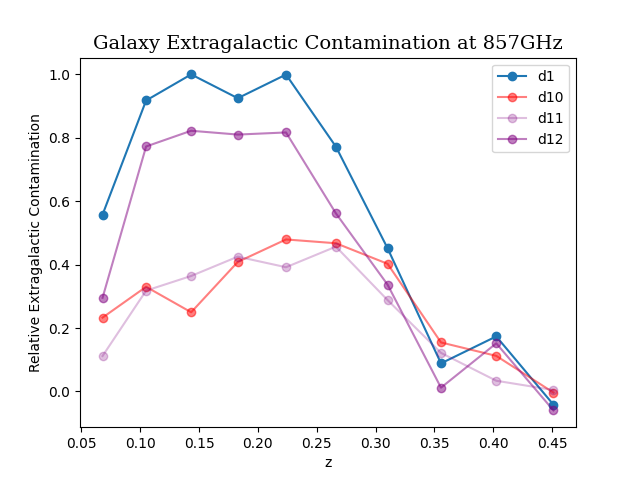
\includegraphics[width=\columnwidth]{figures/EGC_galaxy@857Part_0-1.png}
%     \caption{Relative extragalactic contamination in three of the new dust templates (\texttt{d10, d11, d12}), compared to the \texttt{d1} model. Contamination is quantified as the excess 857 GHz emission within $11'$ of galaxies from the GLADE+ catalog, normalized to the maximum excess and plotted as a function of redshift (z). All three new dust templates contain less extragalactic contamination than older dust models because they are based on GNILC-processed Planck data. The improvement is most significant for \texttt{d10} and \texttt{d11}.  }
%     \label{fig:extragal_contamination}
% \end{figure}


% %Our Galactic dust templates are based on measurements of the 
% We quantify the extragalactic contamination present in our dust models using a tomographic redshift-clustering technique \citep{Schmidt:2015, Chiang:2019}. Our intensity-based Galactic dust templates inevitably contain emission from both Galactic dust and external galaxies. As described in Section \ref{sec:dustamplitude}, the new \texttt{d9} and \texttt{d10} dust templates are derived from GNILC-processed Planck data, while older PySM dust templates used \texttt{Commander} data products. We thus expect that the new Galactic dust models are significantly less affected by CIB contamination than previous models. Here we quantify this contamination by measuring the angular cross-correlation between our dust models and the clustering of galaxies as a function of redshift in spectroscopic survey data. A perfect Galactic dust template would be uncorrelated with such clustering; the signature of CIB contamination is excess template emission correlated with galaxy clustering. 

% Following the procedure in \citet{Chiang:2019}, we compute the cross-correlation between local fluctuations in the Galactic emission maps and the galaxy density as a function of redshift, using galaxies from the GLADE+ catalog \citep{Dalya:2022}. We compute this cross-correlation for each of the \texttt{d1, d10, d11}, and \texttt{d12} dust emission templates at 857 GHz, at high Galactic latitudes ($\left|b\right| > 30\deg$). Figure \ref{fig:extragal_contamination} shows that while each of the new GNILC-based maps contain less extragalactic contamination than \texttt{d1}, the decreased contamination is more marked in \texttt{d10} and \texttt{d11} than in \texttt{d12}. This is likely due to [FILTERING CHOICES? TO DISCUSS WITH JACQUES]


% \subsection{Non-Gaussianity} \label{sec:nongaussianity}
% writing: Yao + Nico

% In this section, we focus on the thermal dust component and investigate the level of non-Gaussianity induced in the small scales generated through the polarization fraction tensor transformation, i.e., the simulations from PySM dust model \deleven{}. We use the Minkowski Functionals (MFs, \cite{Minkowski1903})  to measure the non-Gaussianity in the maps, which have long been used as estimators of non-Gaussianity.

% According to Hadwiger’s theorem\citep{hadwigerVorlesungenUeberInhalt1957}, for any n-dimensional excursion set defined with a threshold value $\rho$, there exists $n+1$ kinds of MFs that geometrically and topologically describe the morphology of the set. Therfore, in our case, for the 2-dimensional maps, we have 3 kinds of MFs, $\mathcal{V}_0$, $\mathcal{V}_1$ and $\mathcal{V}_2$ which corresponds to the area, the length and the connectivity of the excursion set.

% By comparing the MFs of the small scales structures from \deleven{} with those of Gaussian realizations from extrapolated power law, which is fitted from the power spectra of the maps from \deleven{}, in standard $IQU$ domain, we can have a qualitative estimation of non-Gaussianity in \deleven{} introduced by going into $iqu$ domain. As mentioned in Section \ref{subsec:methodology}, the generated small scales in the \deleven{} model are modulated before adding to the large scales. To study the potential effect of anisotropy on the non-Gaussianity, we also generate Gaussian realizations with modulation so that we can compare the non-Gaussianity directly, without the influence of anisotropy. The two reference sets made of pure Gaussian small scales and modulated Gaussian small scales are built as follows:

% \begin{enumerate}

% \item We first fit power laws to the $TT$, $EE$, $BB$ power spectra in the multipole range $[800, 2000]$ calculated from the full sky maps output by \deleven{}, and extrapolate them up to $\ell_{\rm max}=4096$. 
% \item To obtain only the small scales, we apply a high-pass filter to the fitted power law with $\ell_{cut} = 200$ for intensity and polarization maps, and then generate full sky small scales realizations using \texttt{synfast} routine provided by \texttt{HEALPix}. 
% \item For modulated Gaussian maps, these full-sky small scales are then multiplied with modulation maps to have similar anisotropies with the small scales from \deleven{}. While for pure Gaussian maps, we do not apply modulations. 
% \item Meanwhile, the small scales with multipoles larger than 200 in the observed data are filtered out and the large scales remain untouched.
% \item At last, the generated Gaussian small scales are added into observed large scales to form the final set of maps. 
% \end{enumerate}

% Now we have three sets of maps with different small scales co-added: one from \deleven{}, one from pure Gaussian and the last from modulated Gaussian realization in the $IQU$ domain. We then apply a high-pass filter to retain only the small scales of these maps, that we call \texttt{poltens-ss}, \texttt{Gaussian-mod-ss}, and \texttt{Gaussian-ss} respectively. To calculate the MFs we select several patches on the sky and project them onto flat plane. Note that the design of the modulation maps is to ensure the final \texttt{Gaussian-mod-ss} maps have the same anisotropy as \texttt{poltens-ss}, which is done by tuning the modulation maps to let \texttt{Gaussian-mod-ss} have the same power spectra behavior as \texttt{poltens-ss} on different masks that exclude the inner part of the Galactic plane. \texttt{Gaussian-ss} are thought to be fully Gaussian and isotropic. 

% Below we show the MFs calculated for these three sets of small scales on the sphere and also for a selected flat patch.

% \subsubsection{MFs on the sphere}

% Following the algorithm in \cite{2022OJAp....5E..13G}, we calculate the MFs for the three Q maps on the sphere, i.e. \texttt{HEALPix} format, with a Planck HFI 80\% sky mask \footnote{\url{http://pla.esac.esa.int/pla/aio/product-action?MAP.MAP_ID=HFI_Mask_GalPlane-apo2_2048_R2.00.fits}}, which masks out the complex Galactic plane.  Before the calculation we first normalize the maps by dividing each map by its standard deviation separately and choose [-3, 3] as the threshold range to calclate the MFs. Results are shown in Figure.~\ref{fig:MF:sphere}, where the first, second and third kind of MFs are shown from left to right.(MFs of U maps look like very similar to Q maps and are not shown here). 

% We can see that when averaging for large sky fraction, the MFs of \texttt{Gaussian-mod-ss} in blue and \texttt{poltens-ss} in orange are almost the same, while MFs of \texttt{Gaussian-ss} differ a lot in dashed gray color. The difference in MFs between \texttt{poltens-ss} and \texttt{Gaussian-ss} means the existence of non-Gaussianity in \texttt{poltens-ss}, but the similarity between \texttt{poltens-ss} and \texttt{Gaussian-mod-ss} proves that the non-Gaussianity in \texttt{poltens-ss} comes from the anisotropy in the maps, which originates from the modulation, rather than from the polarization fraction tensor transformation.   

% \begin{figure*}[hbt!]
%     \centering
%     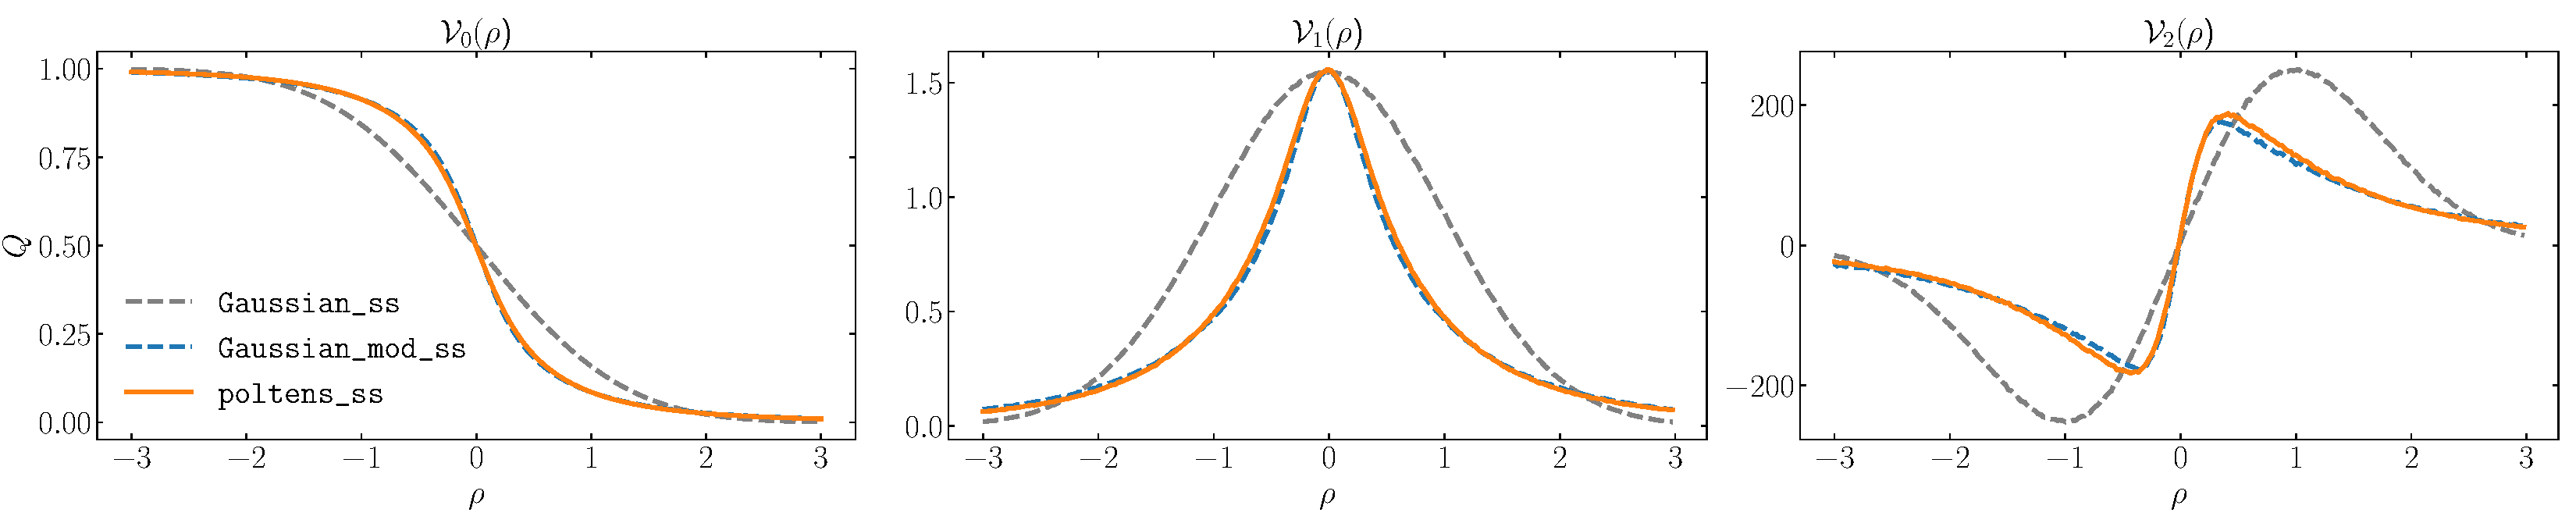
\includegraphics[width=180mm]{figures/MFs_80p_sky_Q.pdf}
%     \caption{MFs for the small scales of three sets of maps on the sphere with Planck HFI 80\% mask. The small scales are filtered out by excluding multipoles smaller than 200 in the maps and we choose $lmax = 2048$ when obaining the small scales. We show the MFs as a function of threshold $\rho$, for \texttt{Gaussian-mod-ss} in blue, \texttt{poltens-ss} in orange and  \texttt{Gaussian-ss} in dashed gray.}
%     \label{fig:MF:sphere}
% \end{figure*}


% \subsubsection{MFs on the flat patch}
% In this section we zoom into a specific region centered at [$-15^{\circ}$ , $45^{\circ} $] with dimension of $20^{\circ}\times20^{\circ}$ to see if, by looking at smaller regions of the sky, we can measure a significance difference in the MFs between \texttt{Gaussian-mod-ss} and \texttt{poltens-ss} sets of maps. Those maps are shown the third and fourth column in Figure~\ref{fig:maps:patch2} respectively, with the Gaussian modulated and \deleven{} full resolution maps including both large and small scales shown in the first and second column. Here we consider I, Q and U maps which are shown from upper to lower panel. When zooming into this patch, we can see by eye that \texttt{poltens-ss} have some structures, following those in the full resolution maps, which are not present in the \texttt{Gaussian-mod-ss} maps. Again we calculate the MFs of these small scales to have an understanding of the non-Gaussianities, following \cite{2008JSMTE..12..015M} for the calculation of MFs for a square patch. Before the calculation, we also rescale all the small scales to be in the range [-1, 1].

% Figure~\ref{fig:MF:patch2} shows the MFs of the \texttt{Gaussian-mod-ss} and \texttt{poltens-ss} maps presented in Figure.~\ref{fig:maps:patch2} as blue and orange lines respectively, while MFs for \texttt{Gaussian-ss} are shown in dashed gray lines. 
% Contrary to the results presented in Figure \ref{fig:MF:sphere}, in this case we can detect a departure of the \texttt{poltens-ss} from the \texttt{Gaussian-mod-ss} ones. This points towards the fact that the polarization fraction tensor transformation may induced some level of non-Gaussianity, different from pure modulation effects, which are detectable on small sky regions. We can thus conclude that the level of induced non-Gaussianity differs from one region to the other and it is in general small enough not to impact significantly the statistical properties when averaged on large sky fraction.  

% \begin{figure*}[hbt]
%     \centering
%     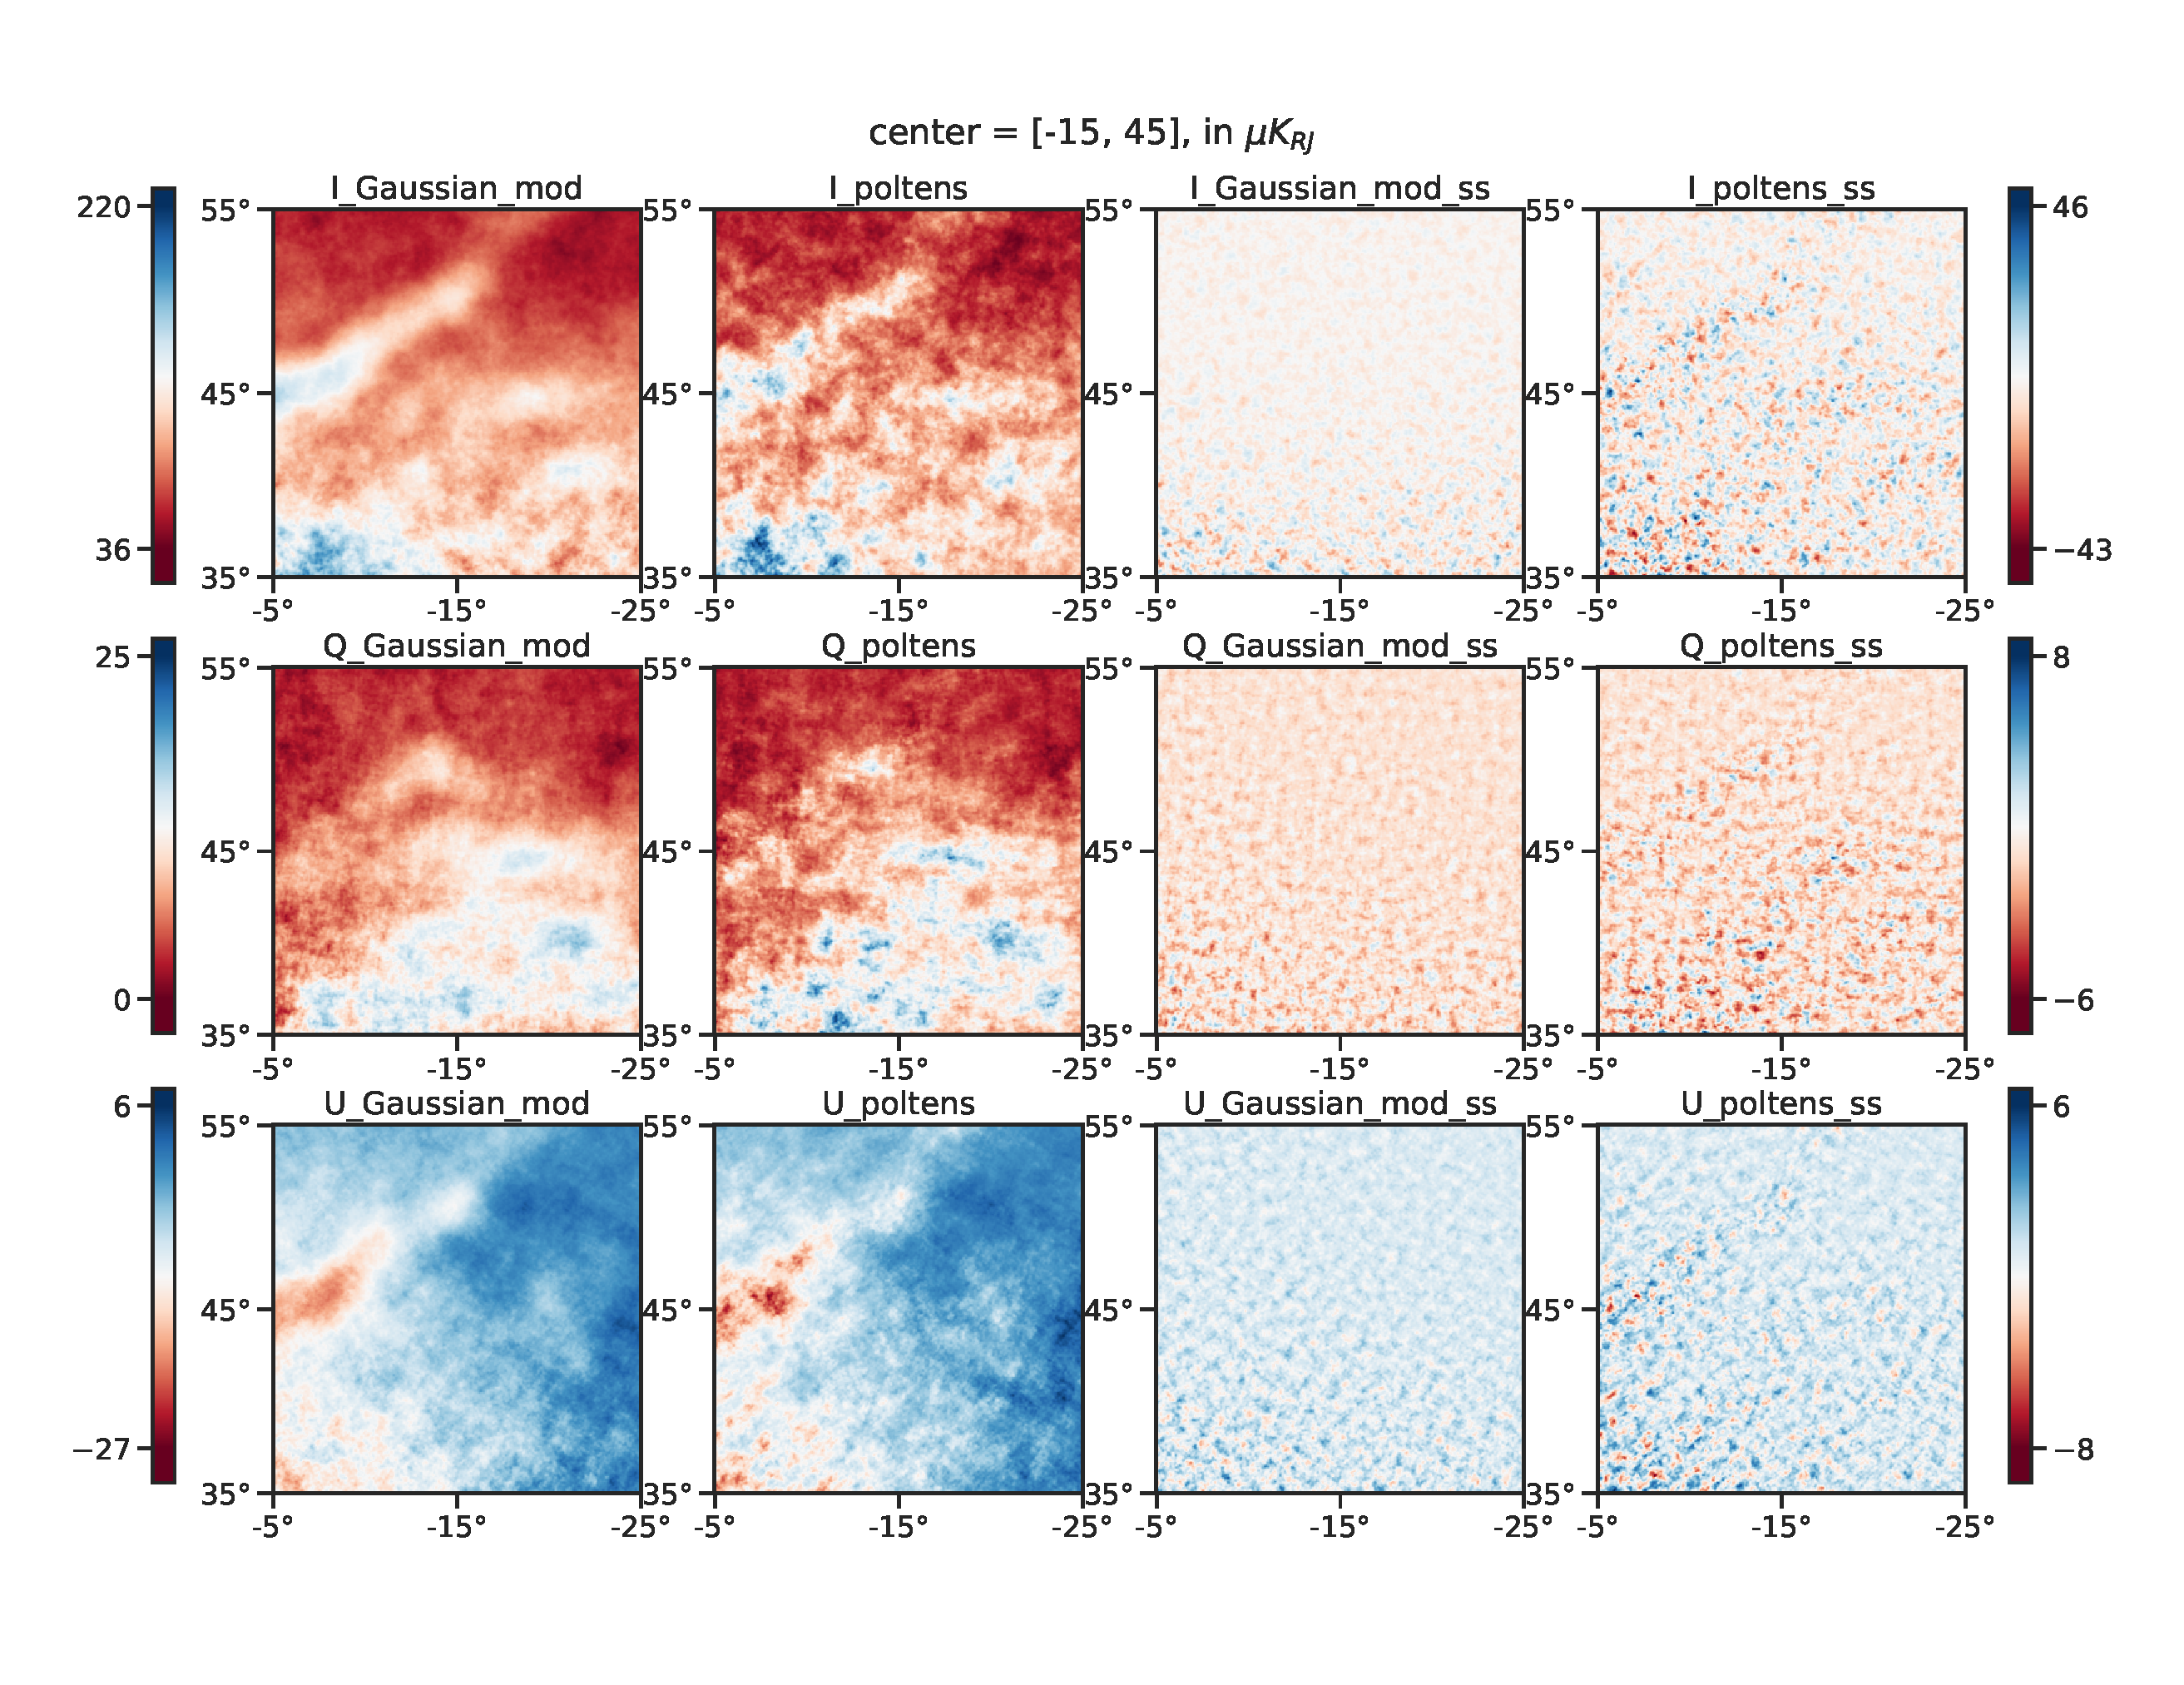
\includegraphics[width=180mm]{figures/maps_patch_345_35.pdf}
%     \caption{The zoom-in plot of the maps, in the selected patch with center [$-15^{\circ}$ , $45^{\circ} $]. From left to right, we show the final map with \texttt{Gaussian-mod-ss}, final map with \texttt{poltens-ss}, \texttt{Gaussian-mod-ss} only map and \texttt{poltens-ss} only map. From top to bottom is for I, Q and U respectively. The colorbar on the left indicates the pixel values in the left-most two columns in the units of $\mu K_{RJ}$ and the colorbar on the right is for the last two columns. }
%     \label{fig:maps:patch2}
% \end{figure*}
% \begin{figure*}[hbt]
%     \centering
%     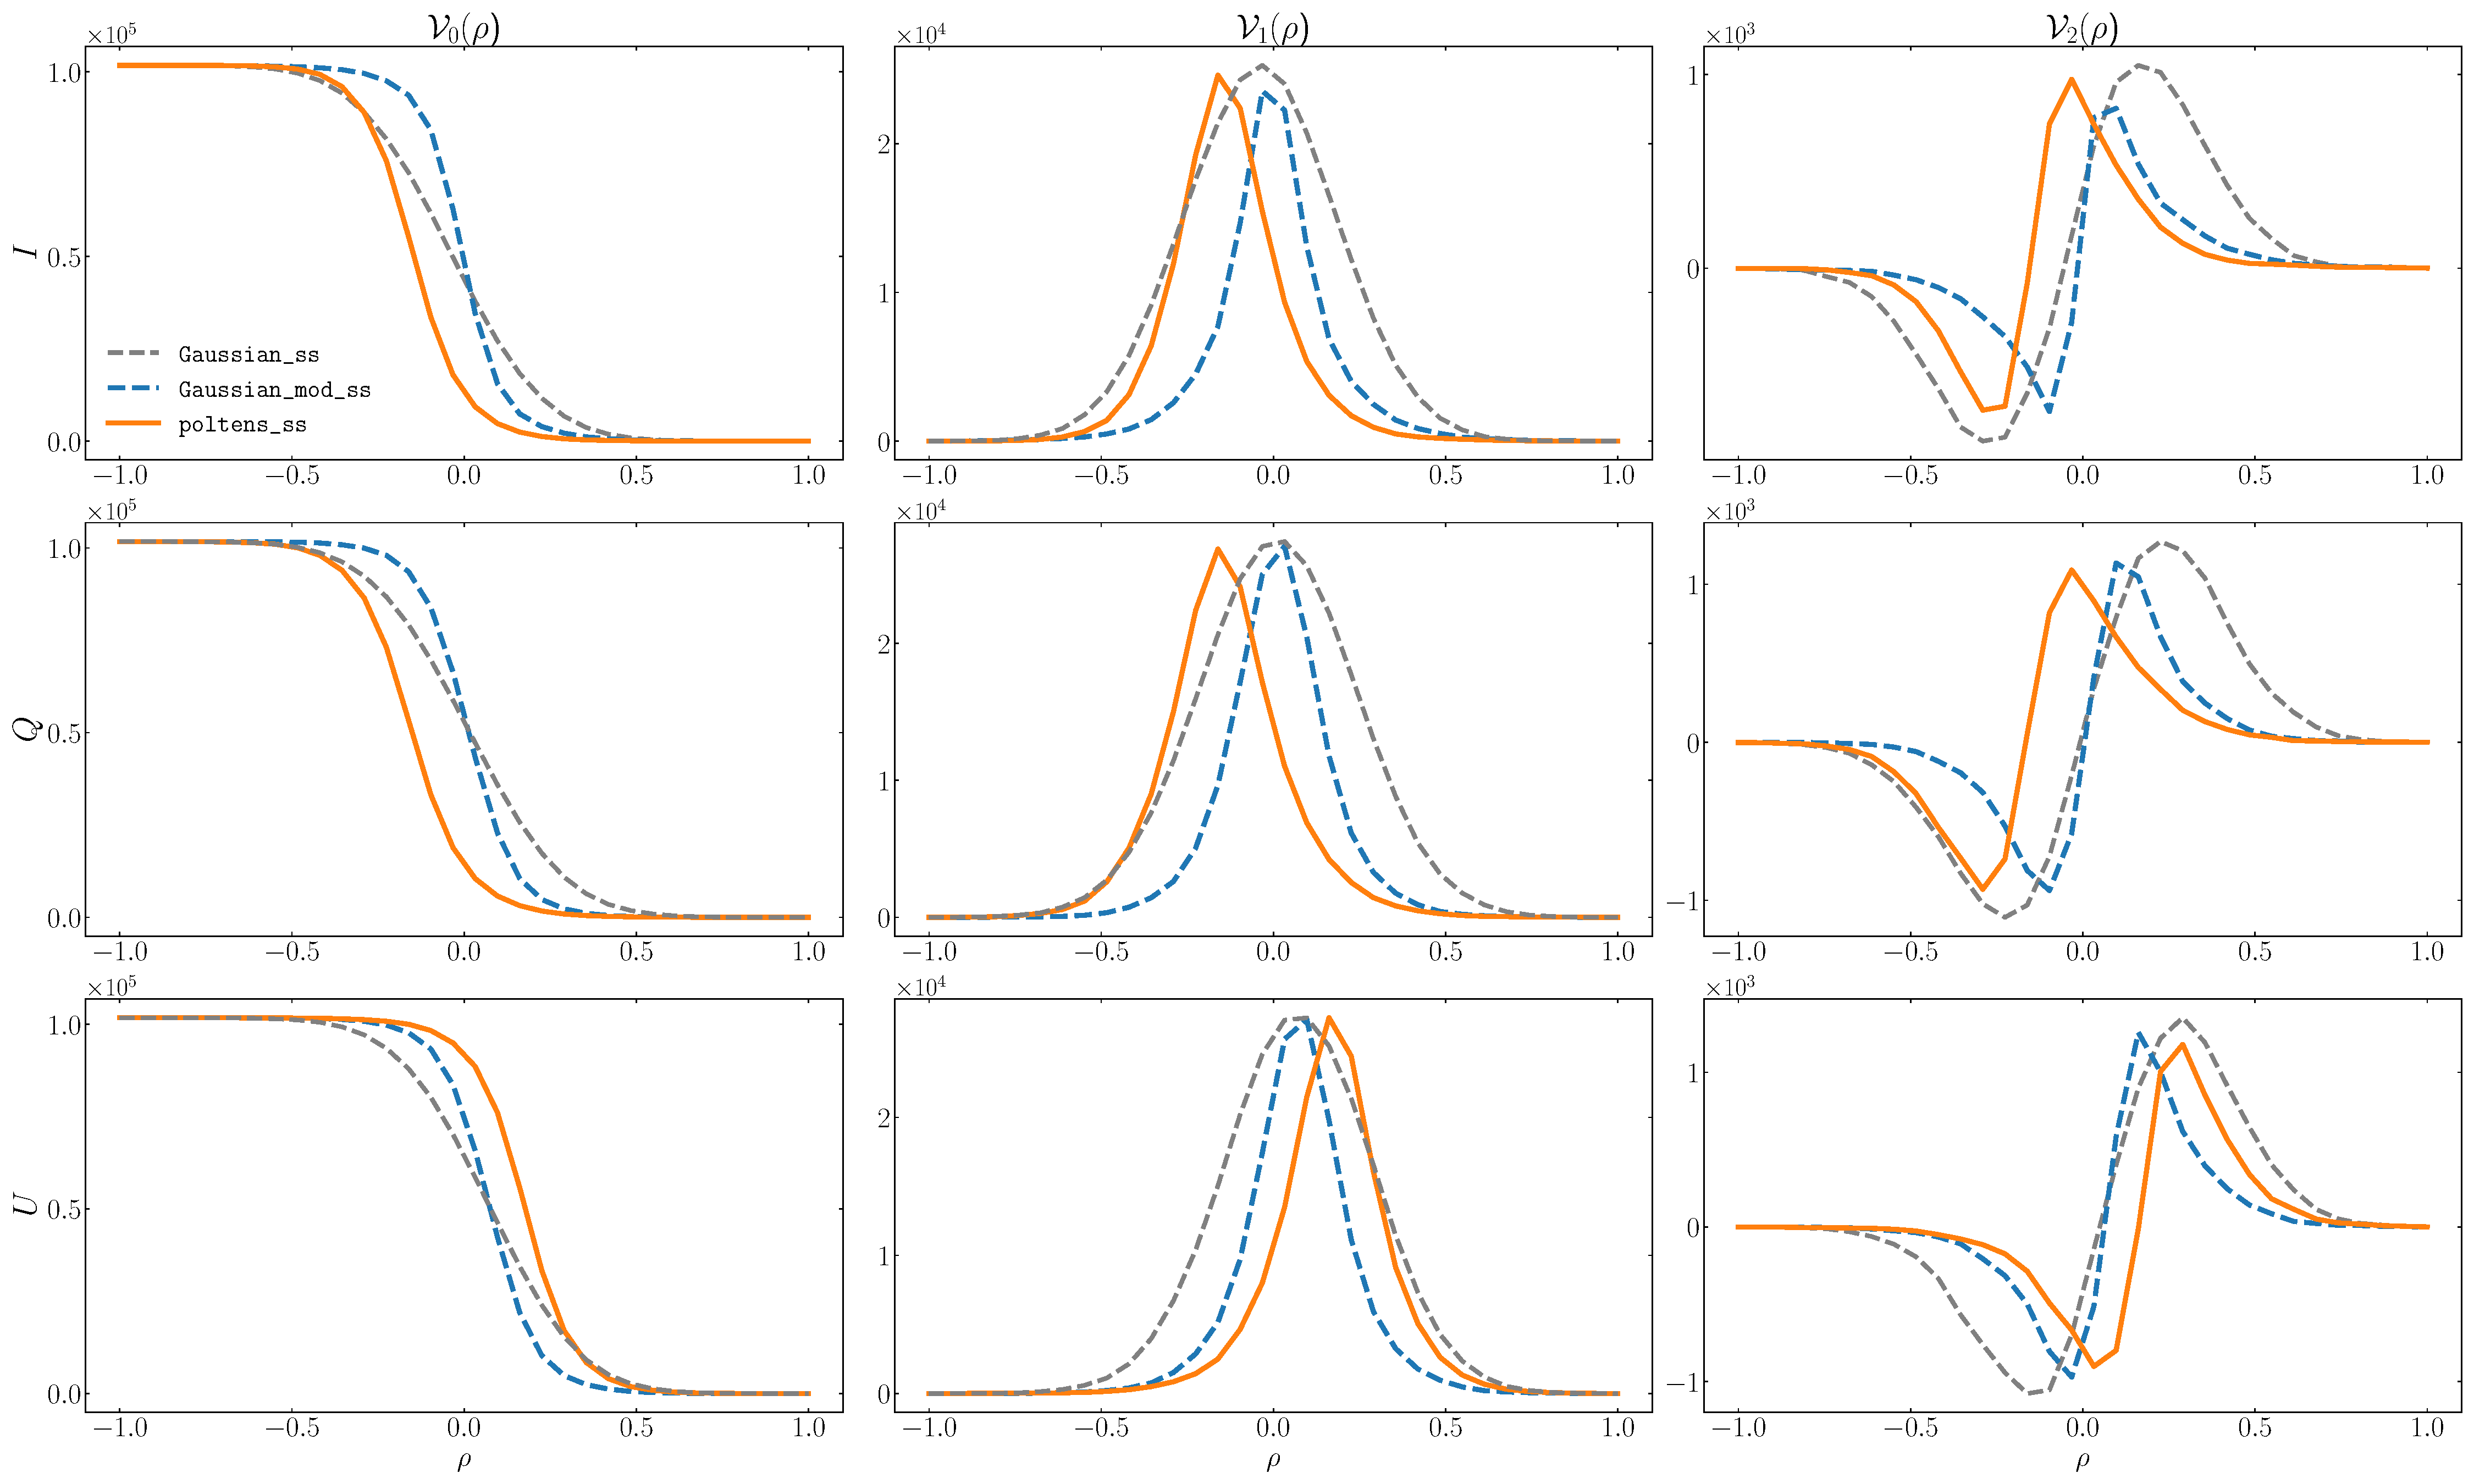
\includegraphics[width=180mm]{figures/MFs_345_45_with_G_rescaled.pdf}
%     \caption{Minkowski Functionals as a function of the threshold $\rho$ for the one realization of I, Q and U small scales in the patch with center of [$-15^{\circ}$ , $45^{\circ} $] in Galactic coordinates. Each row shows three kinds of Minkowski Functionals. The blue dotted one is for \texttt{Gaussian-mod-ss} while the orange solid one is from \texttt{poltens-ss}. We also show the \texttt{Gaussian-ss} in dashed gray line as a comparison.}
%     \label{fig:MF:patch2}
% \end{figure*}


\section{Model Suite}\label{sec:modelsuite}

\begin{table*}[]
    \centering
    \begin{tabular}{lcc}
    
    \toprule 
    Complexity & Model set & Short description \\
    \midrule
    Low  & \texttt{d9, s4, f1, a1, co1} & sdf  \\
    Medium  & \texttt{d10, s5, f1, a1, co3} & sdf   \\
    High  & \texttt{d12, s7, f1, a2, co3} & MKD dust layer model, spatially varying synchrotron curvature, polarized AME  \\
   
   \bottomrule
    \end{tabular}
    \caption{Summary of the suite of model sets described in Section \ref{sec:modelsuite}. These are recommended combinations of models at three levels of complexity (low, medium, and high).  }
    \label{tab:modelsuite}
\end{table*}

The models available for each emission component can be used in various combinations to form a number of unique Galactic sky models. While every user has this combinatoric freedom, we also prescribe a suite of recommended model sets. Table~\ref{tab:modelsuite} details three model sets, representing increasing levels of complexity. The low complexity model set is highly idealized.
The medium complexity model set includes Galactic emission properties that are both expected physically and confirmed observationally, like ..
The high complexity model set models Galactic emission properties that are physically realistic but as-yet undetected, like polarized AME and spatially varying synchrotron curvature. The high complexity model set uses the MKD layer model for Galactic dust emission, and the decorrelation is near the maximum allowed by current constraints.

[Moved from intro, work this in here:]
for example analyzing CMB-S4 data together with that of the precursor South Pole and/or Simons Observatories, or using CMB-S4 high resolution data to help delens LiteBIRD and LiteBIRD high frequency data to help remove dust from CMB-S4.


\section{Discussion} \label{sec:discussion}
writing: Susan + others

\begin{enumerate}
    \item Highlight improvements made and why they are relevant to various CMB science cases
    \item Identify areas where algorithms can be improved (notably modulation of small scales, non-trivial TB/EB correlations)
\end{enumerate}

Susan:
One area for future development is in the implementation of parity-odd polarization quantities ($TB$, $EB$), or effects that give rise to them. The Planck 353 GHz data show a positive $TB$ correlation over large angular scales (cite Planck++), and (misalignment, cite Clark/Huffenberger/Cukierman, state importance for CB++)


\section{Summary and Conclusions} \label{sec:summary}

We have done X. The principal conclusions of this work are as follows:

\begin{enumerate}
    \item Some nice bullets here
\end{enumerate}

Short forward-looking paragraph.

\begin{acknowledgments}

This work was supported by the National Science Foundation under grant No. AST-2106607 (PI S.E.C.). This work was carried out in part at the Jet Propulsion Laboratory, California Institute of Technology, under a contract with the National Aeronautics and Space Administration.

\end{acknowledgments}

\bibliography{refs.bib,refsADS.bib,refsPlanck.bib}

\end{document}
